 
\documentclass [12pt, proquest] {uwthesis}[03/04/2018]
 
\usepackage[noend]{algpseudocode}
\usepackage{algorithm}
\usepackage{alltt}  
\usepackage{amsmath}       % align environment  
\usepackage{dsfont}        % for indicator function
\usepackage{graphicx}      % includegraphic
\usepackage{kbordermatrix} % matrix with element labels
\usepackage{makecell}      % carriage returns in table cells
\usepackage{mathtools}     % shortintertext
\usepackage{natbib}
\def\bibpreamble{\protect\addcontentsline{toc}{chapter}{Bibliography}}

\setcounter{tocdepth}{2}  % Print the chapter and sections to the toc
 

% ==========   Local defs and mods
\newcommand{\blambda}{\boldsymbol{\lambda}}
\newcommand{\bLambda}{\boldsymbol{\Lambda}}
\newcommand{\boeta}{\boldsymbol{\eta}}
\newcommand{\bPhi}{\boldsymbol{\Phi}}
\newcommand{\bmu}{\boldsymbol{\mu}}
\newcommand{\bSigma}{\boldsymbol{\Sigma}}
\newcommand{\btheta}{\boldsymbol{\theta}}
\newcommand{\bA}{\mathbf{A}}
\newcommand{\bF}{\mathbf{F}}
\newcommand{\bM}{\mathbf{M}}
\newcommand{\bW}{\mathbf{W}}
\newcommand{\bN}{\mathbf{N}}
\newcommand{\Ntil}{\widetilde{N}}
\newcommand{\bNtil}{\widetilde{\bN}}
\newcommand{\R}{\mathtt{R}}
\newcommand{\bn}{\mathbf{n}}
\newcommand{\bntil}{\widetilde{\bn}}
\newcommand{\bR}{\mathbf{R}}
\newcommand{\br}{\mathbf{r}}
\newcommand{\bX}{\mathbf{X}}
\newcommand{\bx}{\mathbf{x}}
\newcommand{\bY}{\mathbf{Y}}
\newcommand{\by}{\mathbf{Y}}
\newcommand{\bZ}{\mathbf{Z}}
\newcommand{\bz}{\mathbf{z}}
\newcommand{\e}{\mathrm{e}}
\newcommand{\E}{\mathrm{E}}
\newcommand{\Var}{\mathrm{Var}}
\newcommand{\mcC}{\mathcal{C}}
\newcommand{\mcI}{\mathcal{I}}
\newcommand{\mcS}{\mathcal{S}}
\newcommand{\mcL}{\mathcal{L}}
\newcommand{\mcV}{\mathcal{V}}
\newcommand{\mcO}{\mathcal{O}}
\newcommand{\bs}[1]{\boldsymbol{#1}}
\newcommand{\bm}{\mathbf{m}}
\newcommand{\bV}{\mathbf{V}}
\newcommand{\mr}[1]{\mathrm{#1}}
\newcommand{\mb}[1]{\mathbf{#1}}
\newcommand{\diag}{\mr{diag}}
\newcommand{\rmd}{\mr{d}}
\newcommand{\dt}{\rmd t}
\newcommand{\logit}{\mr{logit}}
\newcommand{\deriv}[2]{\frac{\rmd#1}{\rmd#2}}
\newcommand{\pdiv}[2]{\frac{\partial#1}{\partial#2}}
\newcommand{\doLNA}{\texttt{doLNA}}
\newcommand{\doElliptSS}{\texttt{doElliptSS}}
\newcommand{\ind}[1]{\mathds{1}_{\left \lbrace#1\right \rbrace}}


\renewcommand{\kbldelim}{(}
\renewcommand{\kbrdelim}{)}

\newenvironment{demo}
  {\begin{alltt}\leftskip3em
     \def\\{\ttfamily\char`\\}%
     \def\{{\ttfamily\char`\{}%
     \def\}{\ttfamily\char`\}}}
  {\end{alltt}}
 
% metafont font.  If logo not available, use the second form
%
% \font\mffont=logosl10 scaled\magstep1
\let\mffont=\sf
% --- end-of-sample-stuff ---
 

\begin{document}
 
% Preliminary pages ----------------
\prelimpages

\Title{Bayesian Modeling of Partially Observed Epidemic Count Data}
\Author{Jonathan Fintzi}
\Year{2018}
\Program{Biostatistics}

\Chair{Vladimir Minin}{Co-chair}{}
\Chair{Jon Wakefield}{Co-chair}{}
\Signature{M. Elizabeth Halloran}
\Signature{James Hughes}

\copyrightpage

\titlepage  

\setcounter{page}{-1}
\abstract{%
An incredible abstract with all the best words will appear here.
}
 
\tableofcontents
\listoffigures
\listoftables 
 
\chapter*{Glossary}      % starred form omits the `chapter x'
\addcontentsline{toc}{chapter}{Glossary}
\thispagestyle{plain}
%
\begin{glossary}
\item[AFSS] Automated factor slice sampler.
\item[CTMC] Continuous--time Markov chain.
\item[DA] Data augmentation.
\item[EliptSS] Elliptical slice sampling.
\item[ESS] Effective sample size.
\item[ILI] Influenza--like illness.
\item[LNA] Linear noise approximation.
\item[MJP] Markov jump process.
\item[SEM] Stochastic epidemic model.
\end{glossary}
 

\acknowledgments{% \vskip2pc
  % {\narrower\noindent
  Very grateful to many people. 
  % \par}
}

\dedication{\begin{center}Dedication to important people.\end{center}}



% Text pages -------------
\textpages
\chapter{Introduction}
\label{chap:introduction}

\section{Partially Observed Epidemic Count Data}
\label{sec:data_background}

Outbreak data often consist of aggregate counts reported by public health surveillance systems. The data, which typically reflect the incidence or prevalence of cases in the population, are used to develop an understanding of the outbreak dynamics, assess the effectiveness of interventions, and quantify uncertainty about how the outbreak is likely to evolve. The task of modeling an outbreak is complicated by the limited extent of epidemiological data, which are recorded at discrete observation times, commonly describe just one aspect of the disease process, e.g., infections, and usually capture only a fraction of cases. Complete subject--level data, which would consist of full transmission chains and exact times at which individuals transition through disease states, are rarely available. Asymptomatic cases and imperfect surveillance result in systematic underreporting, which makes it difficult to disentangle whether the data arose from a severe outbreak observed with low fidelity, or a mild outbreak where most cases were detected. The challenges involved in characterizing the outbreak dynamics are often further exacerbated by changes in the outbreak dynamics or surveillance over time, which can reduce the effective amount of available information. Hence, fitting models in the absence of complete data is a complicated missing data/latent variable problem. 

\section{Compartmental Epidemic Models}
\label{sec:outbreak_models}

Compartmental epidemic models are used to describe the dynamics of an outbreak, to estimate how features of the population or environment affect its severity, and to understand how interventions might help to disrupt transmission. A compartmental model represents the time--evolution of an outbreak in terms of the infection histories of individuals as they transition between discrete states, or model compartments. When we use a compartmental model to describe the \textit{transmission} dynamics of an outbreak, the compartments encode structural information about how individuals at different infection states interact to transmit the infectious agent. In contrast, states in a compartmental model for \textit{disease} dynamics typically correspond to discrete stages in the natural history of within--host disease progression without necessarily referring to a host's transmissive potential. 

A compartmental model is referred to as a mechanistic model when it prescribes physical laws that govern the transmission dynamics of an outbreak. For example, the model might specify the rates of infectious contact between classes of individuals, or with an environmental reservoir that is a vector for transmission. The mechanistic structure of the model specifies a functional form for the temporal, and possibly spatial, spread of the epidemic process that is coarsely reflected in incidence and prevalence data. In contrast with their mechanistic counterparts, phenomenological models describe the incidence process without explicitly referring to the physical system that is being observed \cite{chowell2017fitting,chowell2016review}. The price we pay for adopting a mechanistic approach is that our models will be obviously ``wrong", at least in the sense that all models are wrong, so it will be our responsibility to justify their reasonableness. Our reward is that mechanistic models provide us with interpretable, generative descriptions of outbreak dynamics. Moreover, the ubiquity of mechanistic models in the epidemiological literature enables us to incorporate information from previous studies into our own models to inform our prior beliefs about specific aspects of the transmission dynamics. Historical overviews of mechanistic models for disease transmission may be found in \cite{anderson1992infectious,brauer2017mathematical,keeling2008,lessler2016mechanistic}.

Mechanistic compartmental models can be specified at varying levels of fidelity to the underlying epidemic process. Our models will range in granularity, from agent--based models in which we explicitly track the disease histories of individuals, to population--level models defined by the aggregate flow of individuals between model compartments. We refer to a mechanistic model as a stochastic epidemic model (SEM) when we model stochasticity in the epidemic process. Compartmental models with complex dynamics have historically represented the epidemic process as deterministic systems of ordinary or partial differential equations \cite{keeling2008}. All of the models in this dissertation will treat the epidemic process as evolving continuously in time, but observed at discrete times. The decision to work with continuous--time models is advantageous when observation times are not evenly spaced, or when various sub--processes evolve on different time scales \cite{glass2003,shelton2014}. Discrete time models generally produce results that are not independent of the choice time--step, and can be problematic when the census interval of the data and the generation time of the epidemic are misaligned (see \cite{shelton2014} for examples). One (very) compelling reason to prefer discrete time models is that the computational effort required to fit discrete time models can be quite low in settings where it is possible to approximate the transition densities of the epidemic process with common statistical distributions \cite{fisher2017time,held2005}. 

The statistical questions and computational challenges involved in fitting compartmental models are different in small and large population settings. It is particularly important to account for stochasticity in the epidemic process when the population size is small since randomness in the disease process at the subject level can substantially affect the propensity of an infectious agent to spread. As we shall see, fitting a SEM to partially observed count data requires that we enumerate the possible epidemic paths from which the data could have arisen. This can be a daunting task since the set of possible epidemic paths is potentially huge, and the stochastic processes used to model outbreaks in small populations are not always easily amenable to approximation. In contrast, there are many methods for approximating the behavior of outbreaks in large, well--mixed populations that enable us to fit models with complex dynamics. As we shall see, various aspects of these models will interact in complicated ways, so we must think carefully about computation and parameterization. 

In this dissertation, we contribute computational methods for fitting continuous time SEMs to partially observed epidemic count data in both small and large populations. In spite of the rather obvious ubiquity and importance of this data setting, there is a dearth of computational tools for fitting SEMs that are simple, broadly applicable, and computationally robust. The remainder of this chapter provides an overview of the datasets that motivate our methods, which will also serve to outline the organization of this dissertation. 

\section{Motivating Examples}
\label{sec:motivating_examples}

\subsection{Influenza in a British Boarding School}
\label{subsec:bbs_descrip}

In our first application, we will analyze data from an outbreak of influenza in a British boarding school \citep{anon1978, davies1982}. This outbreak took place shortly after the Easter term began in January 1978, and was estimated to eventually infect roughly 90\% of the 763 boys aged 10--18. Daily counts of the boys who were confined to the infirmary from January $22^{nd}$ through February $4^{th}$ were accessed via the \texttt{pomp} package in \texttt{R} \citep{pomp}.

\begin{figure}[htbp]
	\centering
	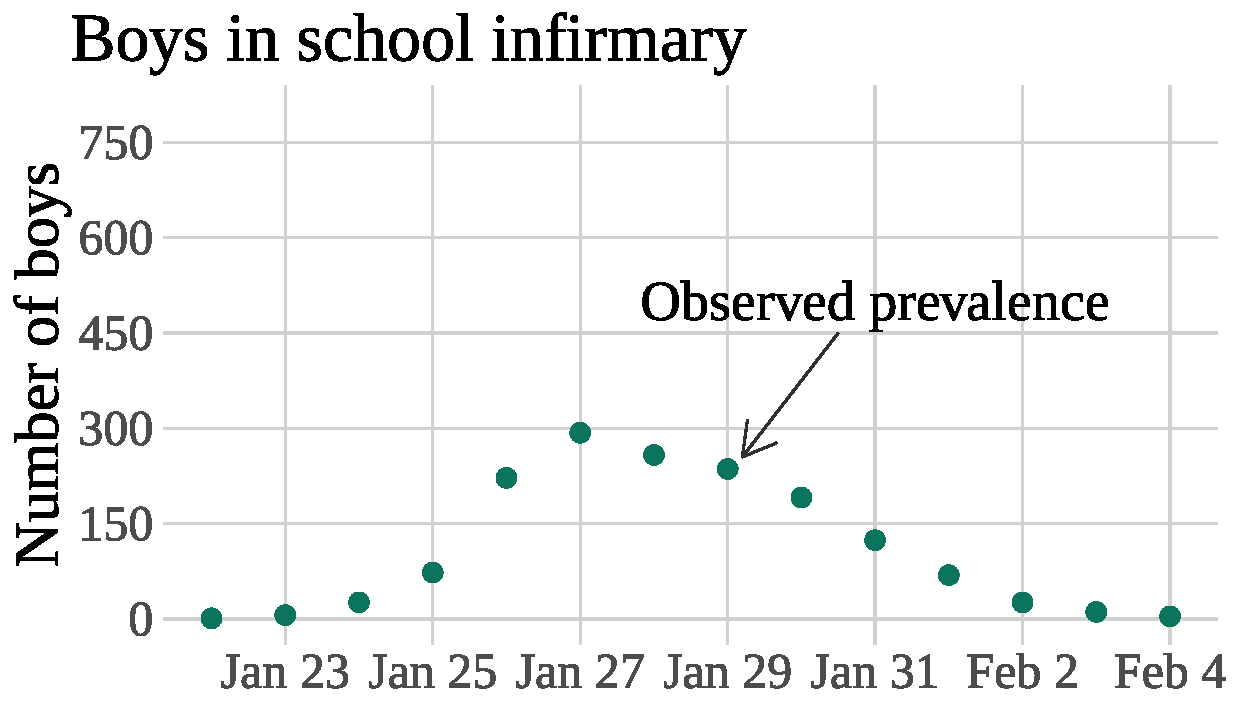
\includegraphics[width=0.6\linewidth]{figures/bbs_data}
	\caption{Data from an outbreak of influenza in a British boarding school.}
	\label{fig:bbsdata}
\end{figure}

Although this dataset is small in scale and duration, reconstructing the true path of the outbreak and describing its dynamics are highly non--trivial inferential tasks. Complicating matters is the lack of individual--level information of any sort, and the possibility that not all of the boys who were infectious on a given day were successfully detected and isolated. In Chapter  \ref{chap:bda_for_fitting_sems_to_prevalence_data}, we present a computationally efficient algorithm for fitting stochastic epidemic models to partially observed prevalence data in small to moderate size populations. This work has been published in Fintzi, et al. (2017) \cite{fintzi2017efficient}. 

\subsection{Epidemics in Large Populations}
\label{subsec:largepop}

\subsubsection{Ebola in West Africa, 2013--2015}
\label{subsec:ebola_descrip}

Starting in December 2013, the West African countries of Guinea, Liberia, and Sierra Leone experienced an outbreak of Ebola that was unprecedented in its size and duration compared to previous Ebola outbreaks. The first cases were thought to have occurred in December 2013 in the Gu\'{e}d\'{e}ckou prefecture in Guinea, while the first cases in Liberia and Sierra Leone were detected on March 30 and June 12, 2014, respectively. By March 2016, a total of 28,646 suspected, probable, and confirmed cases had been reported along with 11,323 deaths \cite{who2016situation}. The outbreak was exacerbated by a number of factors including insufficient outbreak response infrastructure, highly transient populations, and failures to engage with communities early on in the outbreak to implement infection prevention and control measures \cite{coltart2017ebola,dudas2017virus}. 

\begin{figure}[htbp]
	\centering
	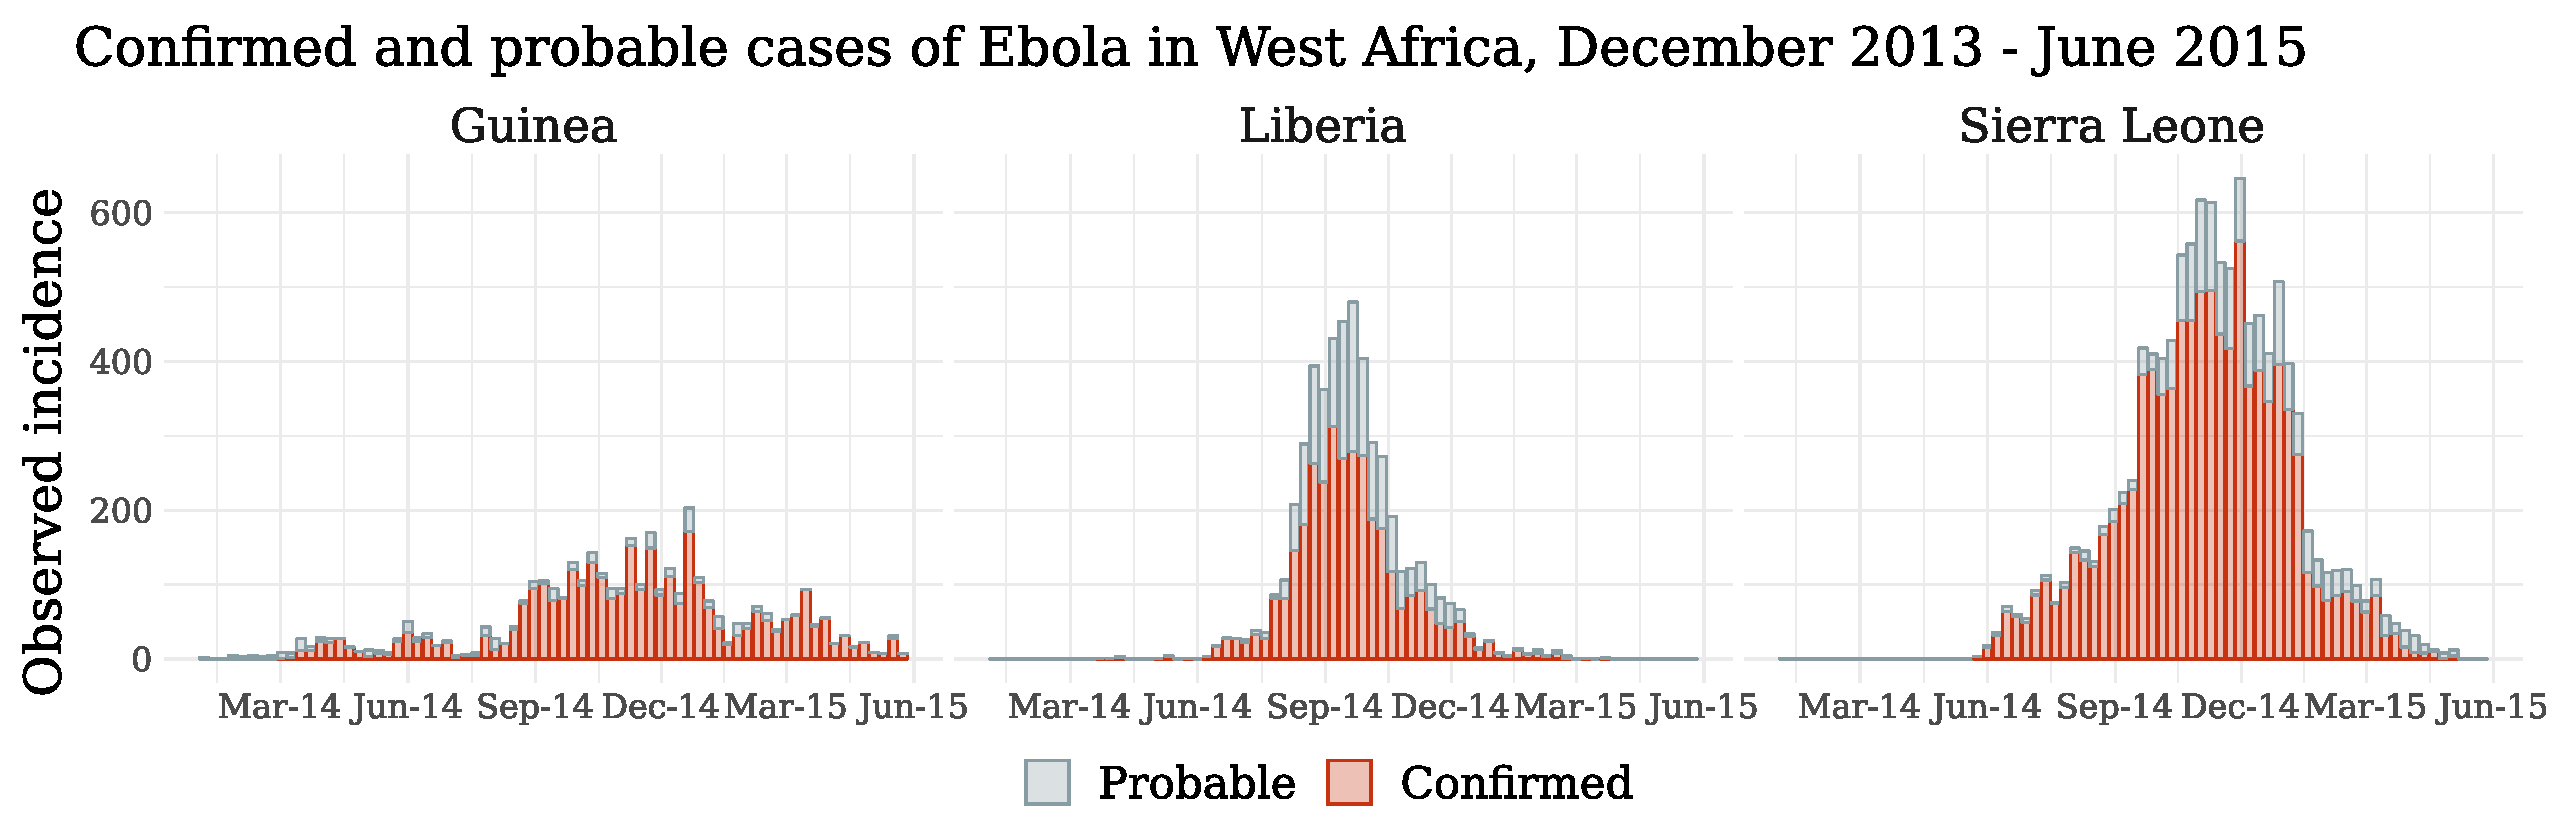
\includegraphics[width=\linewidth]{figures/ebola_dat}
	\caption{Weekly incidence of confirmed and probable cases of Ebola in Guinea, Liberia, and Sierra Leone.}
	\label{fig:eboladat_intro}
\end{figure}

There are several reasons to suspect that the true incidence is significantly under--counted in the dataset. First, suspected cases accounted for sizable fractions of the total case counts, particularly in  Liberia, but were not available as part of this dataset (Table \ref{tab:ebola_descriptives_intro}). Furthermore, analyses based on phylogenetic data \cite{scarpino2014epidemiological} and case fatality ratios \cite{atkins2015under,garske2017heterogeneities} suggest that many cases may have gone undetected, particularly in the early stages, and during the peak, of the outbreak when health systems were overwhelmed. 

\begin{table}[htbp]
	\caption[Ebola incidence by country and case type]{WHO cumulative Ebola incidence by country and case type through May 24, 2015 \cite{who2016eboladat}. Suspected cases were computed as the difference between the official CDC total \cite{cdc2016eboladat}, which included all three case types, and the WHO confirmed plus probable cases.}
	\label{tab:ebola_descriptives_intro}
	\small
	\centering
	\begin{tabular}{lcccc}	
		\hline	
		& \textbf{Guinea} & \textbf{Liberia} & \textbf{Sierra Leone} & \textbf{Total} \\\hline
		\textbf{Confirmed}$ ^1 $ & 3,210 & 3,342 & 9,494 & 16,044\\ 
		\textbf{Probable}$ ^1 $ & 419 & 1,652 & 1,823 & 3,894 \\
		\textbf{Suspected$ ^2 $} & 12 & 5,672 & 1,389 & 7,073 \\
		\hline
		\textbf{Total} & 3,641 & 10,666 & 12,706 & 27,013 \\
		\hline
		\multicolumn{5}{l}{\scriptsize $ ^1 $ Dataset used in the current analysis, cases through 05--24--2015.}\\
		\multicolumn{5}{l}{\scriptsize $ ^2 $ Not available as part of the dataset for this analysis.}\\
	\end{tabular} 
\end{table}

Mathematical models were critical to informing decisions about resource allocation and interventions throughout the outbreak \cite{coltart2017ebola}. A review of 66 modeling studies comprising 125 models for the population--level spread of the outbreak found that modelers typically relied on pre--existing publicly available epidemiological data, which most often consisted of aggregate count data such as weekly incidence counts published by the WHO or national ministries of health \cite{chretien2015mathematical}. Modelers working with incidence data were most often interested in describing the transmission dynamics, particularly the basic reproductive number. Other objectives included forecasting the possible time--evolution of the outbreak, and constructing models to assess the effects of various interventions on the transmission dynamics. Although modeling teams working with publicly available data were not always involved in the policy--making process, the importance of developing outbreak models using real--world data, during what for those teams would be ``peace time", has been emphasized as a critical exercise in preparing for future outbreaks \cite{viboud2018rapidd}.

Analyzing data from the Ebola outbreak presents, in some ways, a fundamentally different challenge compared to the boarding school data. As will become clear, the population sizes of the three countries are far too large for the small population methods in Chapter \ref{chap:bda_for_fitting_sems_to_prevalence_data} to be used. In Chapter \ref{chap:lna_for_sems}, we develop a framework that builds on a linear noise approximation (LNA) for a broad class of compartmental SEMs \cite{fearnhead2014,komorowski2009,ross2009parameter,wilkinson2011stochastic}, and that uses state of the art Markov chain Monte Carlo (MCMC) tools to fit SEMs to partially observed incidence data in large population settings. 

\subsection{Pandemic A(H1N1) Influenza in Finland}
\label{subsec:flu_description}

The emergence of a pandemic influenza A strain, A(H1N1)pdm09, in the spring of 2009 led to widespread concern that it would result in high mortality and excessive stress on public health systems around the world. The strain, commonly referred to as ``swine flu", was a triple reassortment of human, avian, and swine viruses, and was of particular concern because of its similarity to the 1918 pandemic strain that infected up to a third of the world's population and led to an estimated 50 million deaths \cite{cdc1918pandemic}. While the burden imposed by the 2009 pandemic was ultimately comparable to that of seasonal influenza \cite{iuliano2018estimates}, it nevertheless resulted in an estimated 110,000--400,000 respiratory deaths and 50,000--180,000 cardivascular deaths \cite{dawood2012estimated}. The age--standardized cumulative incidence was estimated from serological samples in 19 countries to be between 20\%--27\% of the total population in those countries \cite{van2013estimating}. There was substantial variability in attack rates and transmission dynamics by age, and outbreaks were consistently estimated to be more severe among children and adolescents in terms of cumulative incidence than among adults \cite{opatowski2011transmission,steens2011age,van2013estimating,yang2015inference}. 

We will analyze surveillance data, displayed in Figure \ref{fig:finland_fludat_intro}, from the first and second waves of the epidemic in Finland, where the pandemic A(H1N1) strain was first detected in May, 2009, and where the first wave of the major outbreak began in October, 2009. The dataset, previously analyzed in \cite{shubin2016revealing} and \cite{shubin2014estimating}, consists of weekly counts of laboratory--confirmed A(H1N1) cases, aggregated into sixteen age strata, that were culled from a national surveillance system \cite{lyytikainen2011surveillance}. For computational considerations, we will further aggregate the data into two age groups, individuals ages 0--19 and those of ages 20+, chosen on basis of differences in mixing patterns, susceptibility, vaccination priority, and observed attack rates \cite{kelly2011age,opatowski2011transmission,steens2011age}. All cases in our dataset were of mild severity, i.e., cases that did not require hospitalization. Following \cite{shubin2016revealing,shubin2014estimating}, we treat all A(H1N1) cases as A(H1N1)pdm09 as nearly all A(H1N1) cases were of the pandemic strain. It is critical to note that the data are not marked by vaccination status.

An important aspect of the pandemic response in Finland was the execution of a concerted vaccination campaign with the adjuvanted monovalent vaccine Pandemrix, produced by GlaxoSmithKline. Each resident was offered one vaccine dose, free of charge, starting in October, 2009. Vaccination priority was given to health care workers, vulnerable individuals, and young people under the age of 20 \cite{syrjanen2014effectiveness}. Coverage levels and the timing of vaccination administration varied by age (Figure \ref{fig:finland_fludat_intro}).  Youths under the age of 20 tended to be vaccinated much sooner than adults, and coverage levels among children under the age of 15 were greater than 70\%. Young adults between the ages of 20--29 had the lowest vaccine coverage rates at approximately 30\%. In other settings, vaccine efficacy was found to be higher among children than adults \cite{lansbury2017effectiveness}. Data were not available on vaccine coverage for a trivalent seasonal influenza vaccine administered during the 2010--2011 season. 

\begin{sidewaysfigure}[htbp]
	\centering
	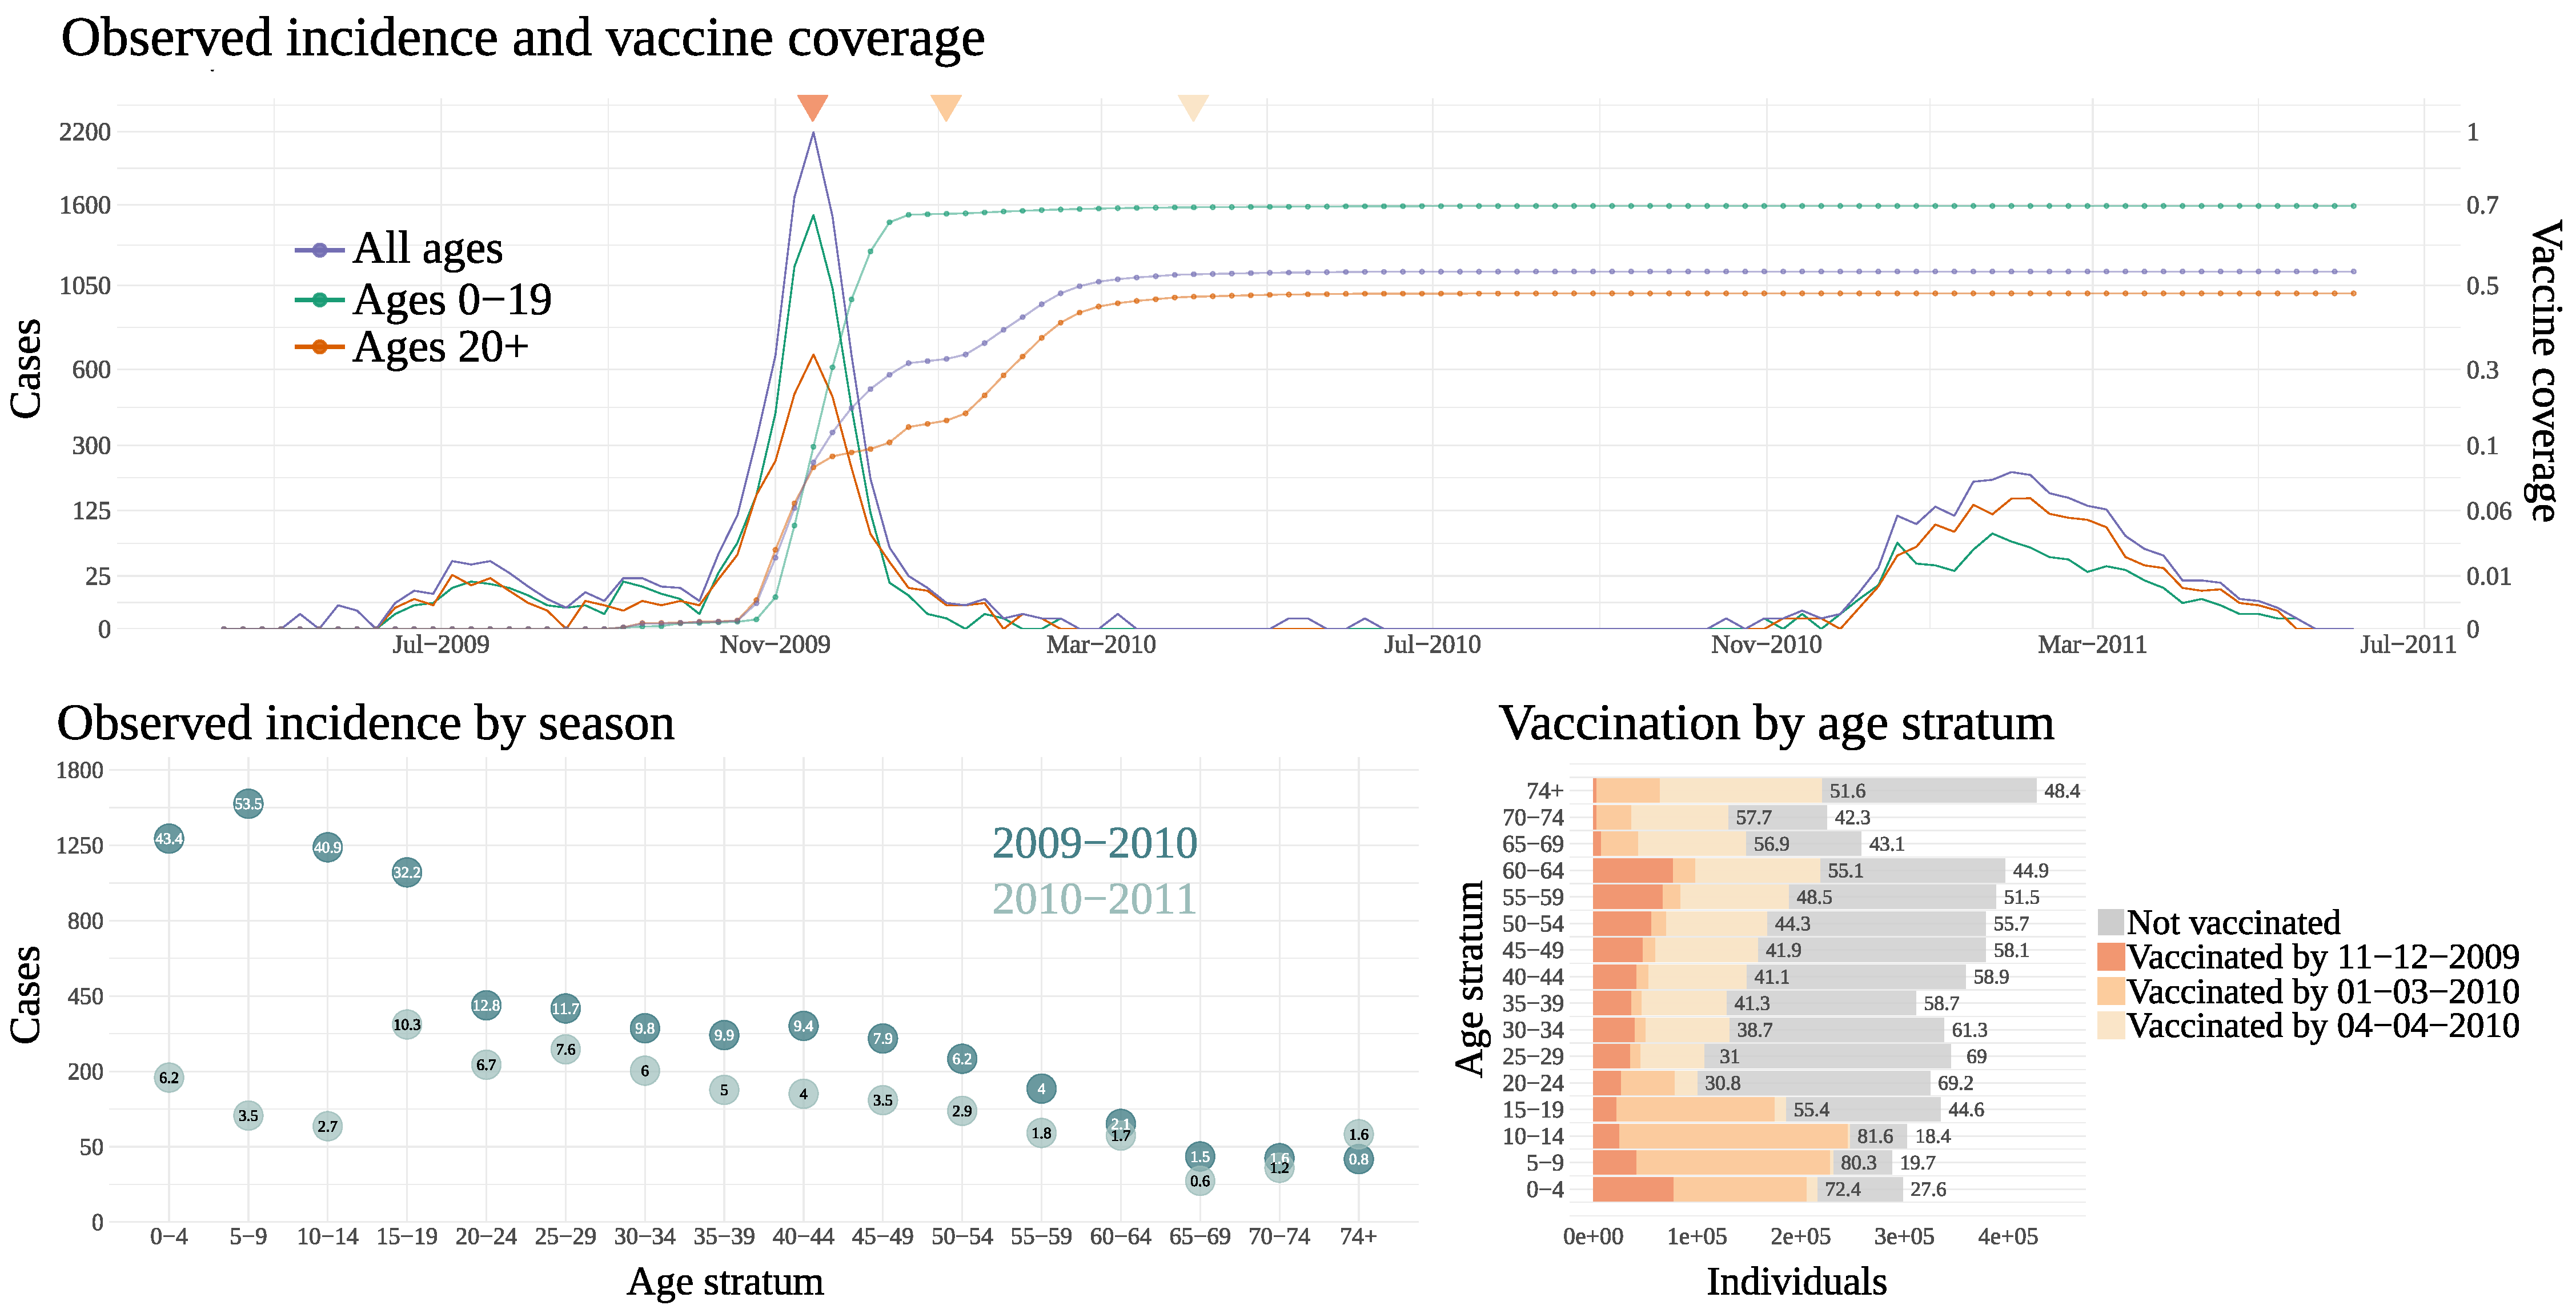
\includegraphics[width=\linewidth]{figures/fludat_plots}
	\caption[A(H1N1)pdm09 incidence and vaccination data from Finland, April 15, 2009 --- June 5, 2011.]{\textbf{Influenza data summaries}. \textit{Top}: Observed incidence (solid lines) and vaccine coverage (lines with points). \textit{Bottom left}: Observed cases by season and age stratum. The 2009--2010 season (dark green) corresponds to the period from April 15, 2009 through April 4, 2010. The 2010--2011 season (light green) corresponds to the period from September 12, 2010 through June 5, 2011. Numbers in points give the attack rate within each stratum for the corresponding season. \textit{Bottom right}: Vaccination coverage by age stratum, colored by vaccine coverages at the times of peak incidence in the first season, tail of the major outbreak in the first season, and end of the vaccination campaign. The numbers inside and outside the histograms denote the percentage of individuals in each stratum that were vaccinated and unvaccinated, respectively, by the end of the vaccination campaign. The times at which vaccine coverages are summarized, denoted by colors of histogram bars, are also identified by corresponding triangles above the top figure.}
	\label{fig:finland_fludat_intro}
\end{sidewaysfigure}

In Chapter \ref{chap:lna_extensions}, we will use methods for approximate inference for SEMs developed and explored in Chapter \ref{chap:lna_for_sems} to fit models with time--varying dynamics. We will then develop an age--vaccination stratified model for the spread of pandemic A(H1N1) in Finland that we will use to pursue three lines of inquiry. First, we will quantify the transmission dynamics and effectiveness of disease surveillance during the first and second seasons. The most important aspect of this involves estimating time--varying reproduction numbers that are interpretable as thresholds for sustained transmission. Second, we will estimate age--specific attack rates and unobserved incidence curves, accounting for underreporting, so that we may better understand the true burden of the pandemic. Finally, we will attempt to understand what effect, if any, the vaccination campaign had in mitigating the severity of the outbreak. % introduction
\chapter{Technical Background}
\label{chap:background}

\section{Mathematical Models for the Spread of Infectious Diseases}
\label{sec:sem_background}

Our objective is to estimate the posterior distribution of parameters, $ \btheta $, that govern the dynamics of an outbreak, given the data $ \bY = (\bY_1,\dots,\bY_L) $, which are accrued at a set of discrete observation times, $ \lbrace t_\ell:\ \ell=1,\dots,L\rbrace $. The data are not independent and typically exhibit complicated temporal (and spatial) dependencies in the data. Therefore, the observed data likelihood in the posterior is not a simple product of independent densities, i.e.,
\begin{align*}
\pi(\btheta|\bY) &\propto\ L(\bY|\btheta)\pi(\btheta) \\
&= \prod_{\ell = 1}^{L} \pi(\bY_\ell|\bY_{1},\dots,\bY_{\ell-1},\btheta)\pi(\btheta) \neq \prod_{\ell = 1}^{L} \pi(\bY_\ell|\btheta)\pi(\btheta).
\end{align*}
Furthermore, the transition density, $ \pi(\bY_{\ell}|\bY_{1},\dots,\bY_{\ell-1}) $, involves a high dimensional integral over an unobserved epidemic process, $ \bX $, 
\begin{equation}
\label{eqn:sem_post}
\pi(\btheta|\bY) \propto \int L(\bY|\bX,\btheta) \pi(\bX|\btheta)\pi(\btheta)\rmd\bX.
\end{equation}
This integral is analytically intractable when the state space of $ \bX $ is of even moderate size. Simply put, it is difficult to enumerate how the data could have arisen, given the vastness of possibilities for how an unseen outbreak might have evolved. 

In this dissertation, we will describe the latent epidemic process using continuous--time models that possess the Markov property, meaning that the forward--time evolution of the latent process depends on its history only through its current state. This choice reduces the structure of (\ref{eqn:sem_post}) to that of a hidden Markov model wherein the data are conditionally independent given the latent epidemic process (diagrammed in Figure \ref{fig:semhmm}). The  posterior is 
\begin{align}
\label{eqn:sem_post_hmm}
\pi(\btheta|\bY) &\propto\int \prod_{\ell = 1}^{L} L\left (\bY_\ell|\bX(t_{\ell}),\btheta\right ) \pi\left (\bX(t_\ell)|\bX(t_{\ell-1}),\btheta\right )\pi(\btheta)\rmd\bX.
\end{align}
On its own, this might seem to solve nothing. The integral in (\ref{eqn:sem_post_hmm}) is still analytically intractable, and the state space of $ \bX $ is still too large to easily work with the augmented posterior, 
\begin{equation}
\pi(\btheta,\bX|\bY)\propto L(\bY|\bX,\btheta)\pi(\bX|\btheta)\pi(\btheta).
\end{equation}
However, this choice also creates symmetries in the ways that individuals interact and contribute to the outbreak dynamics. This additional structure is critical in facilitating efficient computation. In the following sections, we present a number of representations for the latent epidemic process, and conclude with a brief overview of computational approaches for inference.  

\begin{figure}[htbp]
	\centering
	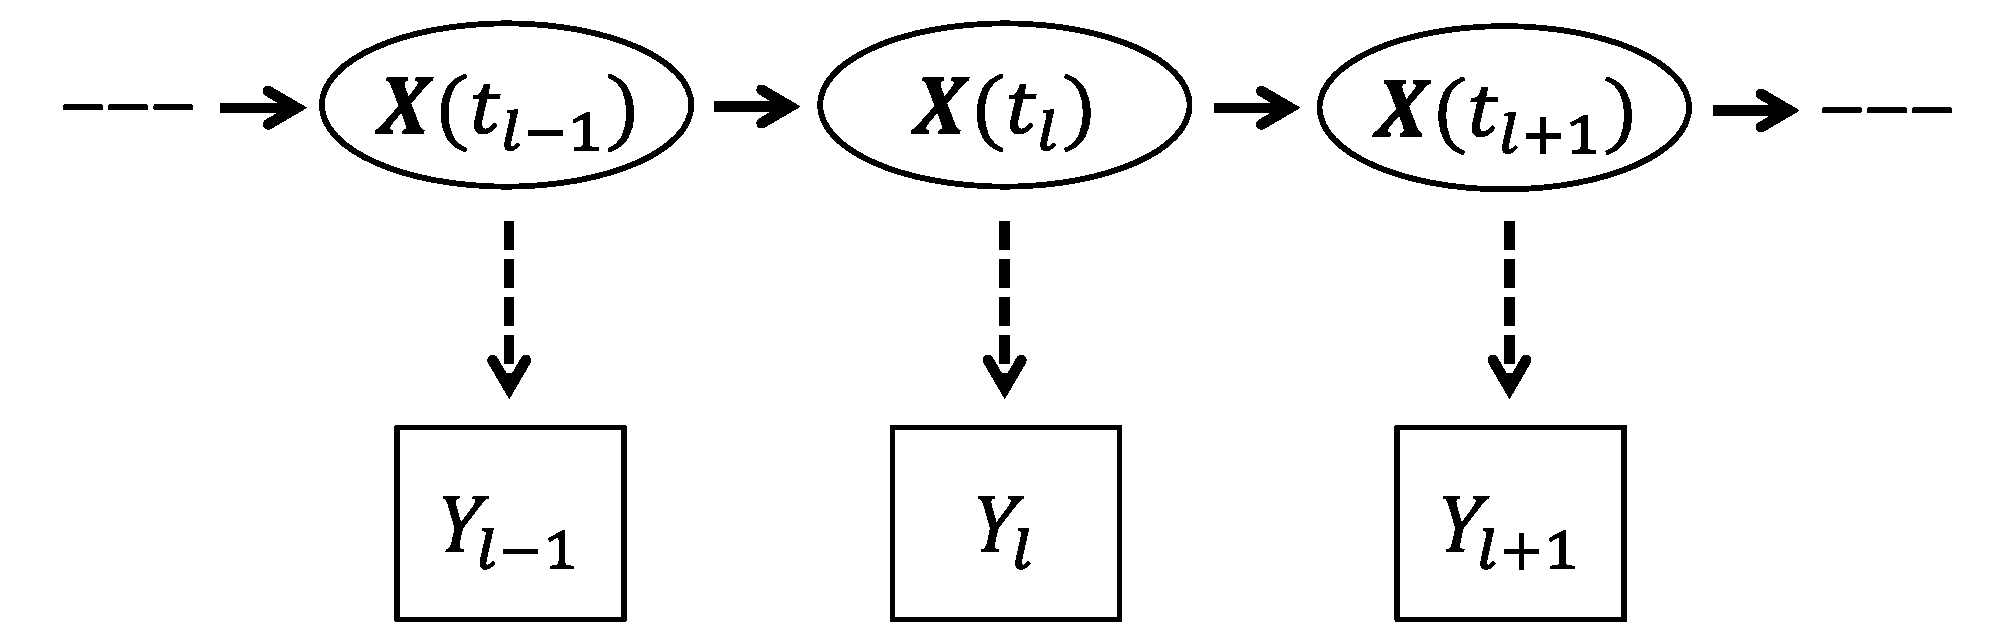
\includegraphics[width=0.5\linewidth]{figures/SEM_HMM}
	\caption[Diagram of a Hidden Markov model.]{Diagram of a Hidden Markov model. The data are conditionally independent given the latent epidemic process.}
	\label{fig:semhmm}
\end{figure}

\subsection{An Agent--Based Susceptible--Infected--Recovered Model}
\label{subsec:sir_individual_mod}
For clarity of exposition, we will present the technical background on epidemic models in terms of the susceptible--infected--recovered (SIR model). Formal treatments that deal with this material in greater generality can be found in \cite{andersson2000stochastic,britton2018,brauer2008compartmental,fuchs2013inference,greenwood2009stochastic,wilkinson2011stochastic}. The SIR model classifies individuals in a population of size $ N $ into one of three infection states: susceptible (S), infected (I), and recovered (R). Individuals are assumed to become infectious immediately upon entering the infected state, and acquire lasting immunity upon recovery. To simplify matters, we will assume the population is closed, meaning that there are no demographic changes or immigration, and that individuals are exchangeable. This latter assumption implies that individuals mix homogeneously and are alike in their infection dynamics. 

The SIR model defines an epidemic process, $ \bX = \lbrace\bX_1,\dots,\bX_N\rbrace $, that collects the subject--level subprocesses, $ \bX_j,\ j=1,\dots,N $, each of which takes values in the state space of disease state labels, $ \mcS_j= \lbrace S,I,R\rbrace $. A realized subject--path is of the form 
\begin{equation}
\bx_j = \left \lbrace\begin{array}{ll}
S,\ & \tau < \tau_I^{(j)},\\
I,\ & \tau_I^{(j)}\leq\tau<\tau_R^{(j)},\\
R,\ & \tau_R^{(j)} \leq \tau,
\end{array}\right .
\end{equation}
where $ \tau_I^{(j)} $ and $ \tau_{R}^{(j)} $ are the infection and recovery times for subject $ j $, and are possibly infinite (Figure \ref{fig:subjectsamplepaths}). The state space of $ \bX $ is  $ \mcS = \lbrace S,I,R\rbrace^N $, the Cartesian product of subject--level state labels. We denote by $ \bX(\tau) = \left (\bX_1(\tau),\dots,\bX_N(\tau)\right ) $ the state of $ \bX $ at time $ \tau $, and by $ \bX(\tau^+) $ the state just after time $ \tau $. 

\begin{figure}[htbp]
	\centering
	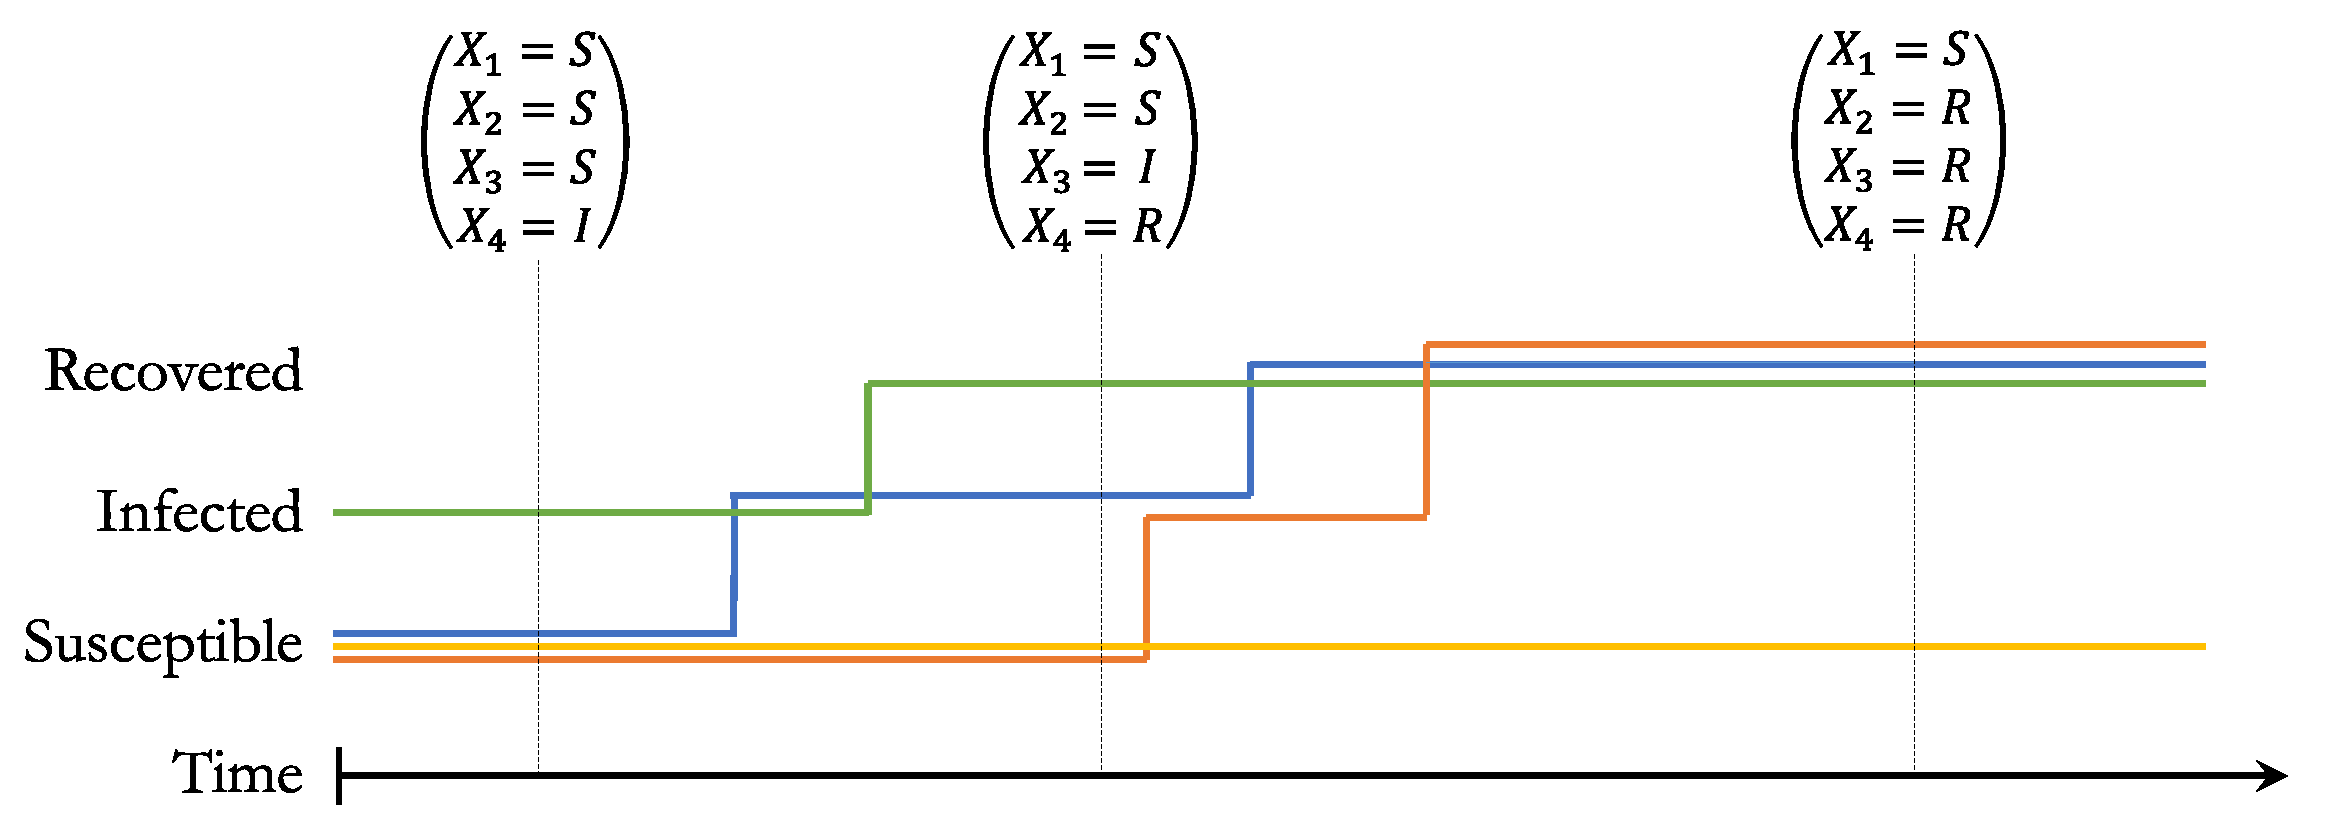
\includegraphics[width=0.8\linewidth]{figures/subject_sample_paths}
	\caption[Diagram of subject--level SIR paths.]{Diagram of subject--level paths (colored lines) for an SIR model in a population of size $ N=4 $. Individuals transition through infection states continuously in time. The epidemic process is defined in terms of the infection states of individuals in the population.}
	\label{fig:subjectsamplepaths}
\end{figure}

The waiting times between subject--level transition events are typically taken to be exponentially distributed. This will allow us to take advantage of several useful properties of exponential random variables (Figure \ref{fig:exp_props}, see \cite{wilkinson2011stochastic} for proofs). Critically, this choice also implies that $ \bX $ evolves as a continuous--time Markov chain (CTMC) with transition rate from configuration $ \bX $ to $ \bX^\prime $, differing only in the state of a single subject, given by
\begin{equation}
\lambda_{\bX,\bX^\prime} = \left \lbrace \begin{array}{rl}
\beta I,\ &\text{if } \bX\ \text{and } \bX^\prime\ \text{differ only in subject }j \text{, with }\bX_j=S\text{, and }\bX_j^\prime=I,\\
\mu,\ &\text{if } \bX\ \text{and } \bX^\prime\ \text{differ only in subject }j \text{, with }\bX_j=I\text{, and }\bX_j^\prime=R,\\
0,\ & \text{for all other configurations }\bX\ \text{and }\bX^\prime.
\end{array}\right.
\end{equation}
with per--contact infection rate,  $ \beta $, and recovery rate, $ \mu $. The quantity, $ 1/\mu $, is interpreted as the mean infectious period duration. That $ \bX $ is a \textit{Markov} process means that its forward--time evolution depends on its history only through its current state, i.e.,
\begin{equation}
\label{eqn:sir_markov}
\Pr\left (\bX(\tau + \dtau) = \bx^\prime | \lbrace\bX(\tau) = \bx,\ \tau\in[0,\tau]\rbrace, \btheta\right ) = \Pr\left (\bX(\tau + \dtau) = \bx^\prime | \bX(\tau) = \bx,\btheta\right ),
\end{equation}
where $ \bx^\prime,\bx \in \mcS$. $ \bX $ is \textit{time--homogeneous} since the rates of transition between configurations in the state space of $ \bX $ are constant over time. 

\begin{framed}
	\begin{itemize}
		\begin{lstlisting}[caption={Useful properties of exponential random variables.},label={list:exp_props}]
		\end{lstlisting}
		\item (Memoryless property) If $ Z\sim\mr{Exp}(\lambda)$, then $ \forall t,\dt\geq0 $  we have \begin{equation}\label{eqn:memoryless_prop}
		\Pr(Z > t+\dt | Z>t) = \Pr(Z>\dt).
		\end{equation}
		\item (Racing exponentials) If $ Z_i\sim\mr{Exp}(\lambda_i),\ i=1,\dots,n $, are independent, then \begin{equation}\label{eqn:racing_exponentials}
		\underset{i}{\mr{min}}(Z_i) \sim \mr{Exp}\left (\lambda = \sum_i\lambda_i\right ).
		\end{equation}
		\item (Index of minimum) If $ Z_i\sim\mr{Exp}(\lambda_i),\ i=1,\dots,n $, are independent, then the index $ k $ of the minimum of $ Z_i $ is a random variable with probability mass function \begin{equation}\label{eqn:ind_of_min}
		\Pr(k|Z_k = \min(Z_1,\dots,Z_n)) = \frac{\lambda_k}{\sum_j\lambda_j}.
		\end{equation} 
	\end{itemize}
\end{framed}

Let $ \btau = \lbrace\tau_0,\dots,\tau_{K+1}\rbrace $, be the (ordered) set of $ K $ infection and recovery times of all individuals along with the endpoints of the time period $ [\tau_0,\ \tau_{K+1}] $. Let $ \ind{\tau_k \corresponds I} $ and $ \ind{\tau_k \corresponds R} $ indicate whether $ \tau_k $ is an infection or recovery time, and let $ \btheta = (\beta, \mu, \bX_0) $ denote the vector of parameters, including the initial state of $ \bX $ at time $ \tau_0 $. The CTMC likelihood of $ \bX $ over $ [\tau_0,\ \tau_{K+1}] $ is a product of exponential waiting time densities,
\begin{align} 
\label{eqn:sir_subj_likelihood}
L(\bX| \btheta) &= \prod_{k = 1}^{K}\left \lbrace \left [\beta I_{\tau_k}\times\ind{\tau_k \corresponds I} + \mu\times\ind{\tau_k \corresponds R}\right ] \exp{\left [-\left (\tau_k - \tau_{k-1}\right )\left (\beta I_{\tau_k} S_{\tau_k} + \mu I_{\tau_k}\right )\right ]}\right \rbrace \nonumber \\
& \hspace{0.2in} \times \exp \left [-\left (t_L - \tau_K\right )\left (\beta I_{\tau_K^+}S_{\tau_K^+} + \mu I_{\tau_K^+}\right )\right ]. 
\end{align}

In contrast with the population--level CTMC, $ \bX $, the subject--level subprocess, $ \bX_j $, is a \textit{time--inhomogeneous} CTMC with transition rate matrix
\begin{equation} 
\label{eqn:sir_subj_rate_mtx}
\bLambda^{j}(\btheta)(\tau) = \bordermatrix{ & S & I & R \cr
	S & -\beta I^{(-j)}(\tau) & \beta I^{(-j)}(\tau) & 0 \cr 
	I & 0 & -\mu & \mu \cr
	R & 0 & 0 & 0 },
\end{equation}
since $ I^{(-j)}(\tau) $, the number of infected individuals in the population at time $ \tau $, excluding individual $ j $, changes over time. We could also describe $ \bX_j $ as piecewise--homogeneous since the rate of infection for subject $ j $ is constant between times at which other individuals become infected and recover. 

\subsection{A Population--Level Susceptible--Infected--Recovered Model}
\label{subsec:sir_population_mod}
The subject--level SIR model is equivalent to an aggregated SIR model, expressed in terms of compartment counts \cite{allen2008introduction, andersson2000stochastic}. This equivalence derives from two properties of Markov processes, \textit{lumpability} and \textit{commutativity}. The population--level SIR model is usually presented for computational reasons since discarding the subject labels associated with infections and recoveries substantially reduces the computational burden of caching subject--level paths. We refer to \cite{tian2006lumpability} for a more formal presentation of the following discussion. 

Given a Markov process, $ \bX $ with state space $ \mcS = \lbrace s_1,\dots,s_P\rbrace $ and initial probability vector $ \pi $, we define another process, $ \overline{\bX} $ on the state space $ \overline{\mcS} = \lbrace S_1,\dots,S_\mathcal{L}\rbrace $, which is a \textit{partition} of $ \mcS $. In our setting, the partitioning will map a configuration in $ \mcS $ to a set in $ \overline{\mcS} $ by counting the number of people in each model compartment. The jump chain of the new process is obtained by partitioning the jump chain of the complete process. We want to establish conditions under which $ \overline{\bX} $ is stochastically coupled to $ \bX $. 

Suppose the initial distribution of $ \overline{\bX}(t_0) $, induced by the distribution of $ \bX(t_0) $, is \begin{equation*}
\Pr(\overline{\bX}(t_0) = S_i) = \mathrm{Pr}_\pi(\bX(t_0) \in S_i)
\end{equation*}
and that its transition probabilities are
\begin{equation*}
\Pr(\overline{\bX}(t+\Delta t) = S_j | \overline{\bX}(t)=\overline{\bx}(t^\prime), t^\prime \leq t) = \Pr(\overline{\bX}(t+\Delta t) \in S_j | \bX(t)=\bx(t^\prime), t^\prime \leq t),
\end{equation*}
where $ \overline{\bx}(t^\prime) $  and $ \bx(t^\prime) $ denote the paths of the complete Markov process and the new process. We say that the complete Markov process is \textit{lumpable} with respect to a partition, $ \overline{\mcS} $, of its state space if lumping the complete process results in a Markov process with respect to the lumped state space for every choice of $ \pi $ whose transition probabilities do not depend on $ \pi $. We refer to the process obtained by lumping as the \textit{lumped} Markov jump process (MJP). If the jump chain of the lumped MJP is the same as the lumped jump chain of the complete MJP, we say that the complete process is \textit{commutative} with respect to lumping.  

Let $ S_A $ and $ S_B $ be elements of $ \overline{\mcS} $, i.e., sets of states $ s_j \in \mcS $. The rate matrix of a CTMC is lumpable if
\begin{equation*}
\sum_{s_b \in S_B}\lambda_{s_a,s_b} = \sum_{s_b \in S_B}\lambda_{s_c,s_b}
\end{equation*}
for any pair of sets $S_A,S_B \in \overline{\mcS} $ and any pair of states  $(s_a, s_c) \in S_A$. A Markov process $ \bX $ is lumpable with respect to a partition of its state space if and only if its rate matrix is lumpable. Lumpability implies that transition probabilities for the lumped chain can be computed based on the lumped rate matrix  \cite{tian2006lumpability}.

Suppose $ \bX $ is lumpable with respect to the partition $ \overline{\mcS} $ of $ \mcS $. Then $ \bX $ is commutative with respect to the partition if and only if the rate matrix of $ \bX $ satisfies
$$\lambda_{s_a,s_b} = 0,\ \text{if}\ s_a,s_b\in S_A,\ \text{and}\ s_a\neq s_b. $$ In our context, commutativity means that the transition rate is zero between different configurations $ \bx_a $ and $ \bx_b $ with equal compartment counts. Commutativity implies that lumped quantities of interest for $ \bX $, such as transition rates or transition probabilities, can be equivalently computed based on $ \bX $, or based on the lumped process, $ \overline{\bX} $ \cite{tian2006lumpability}. 

\begin{figure}
	\centering
	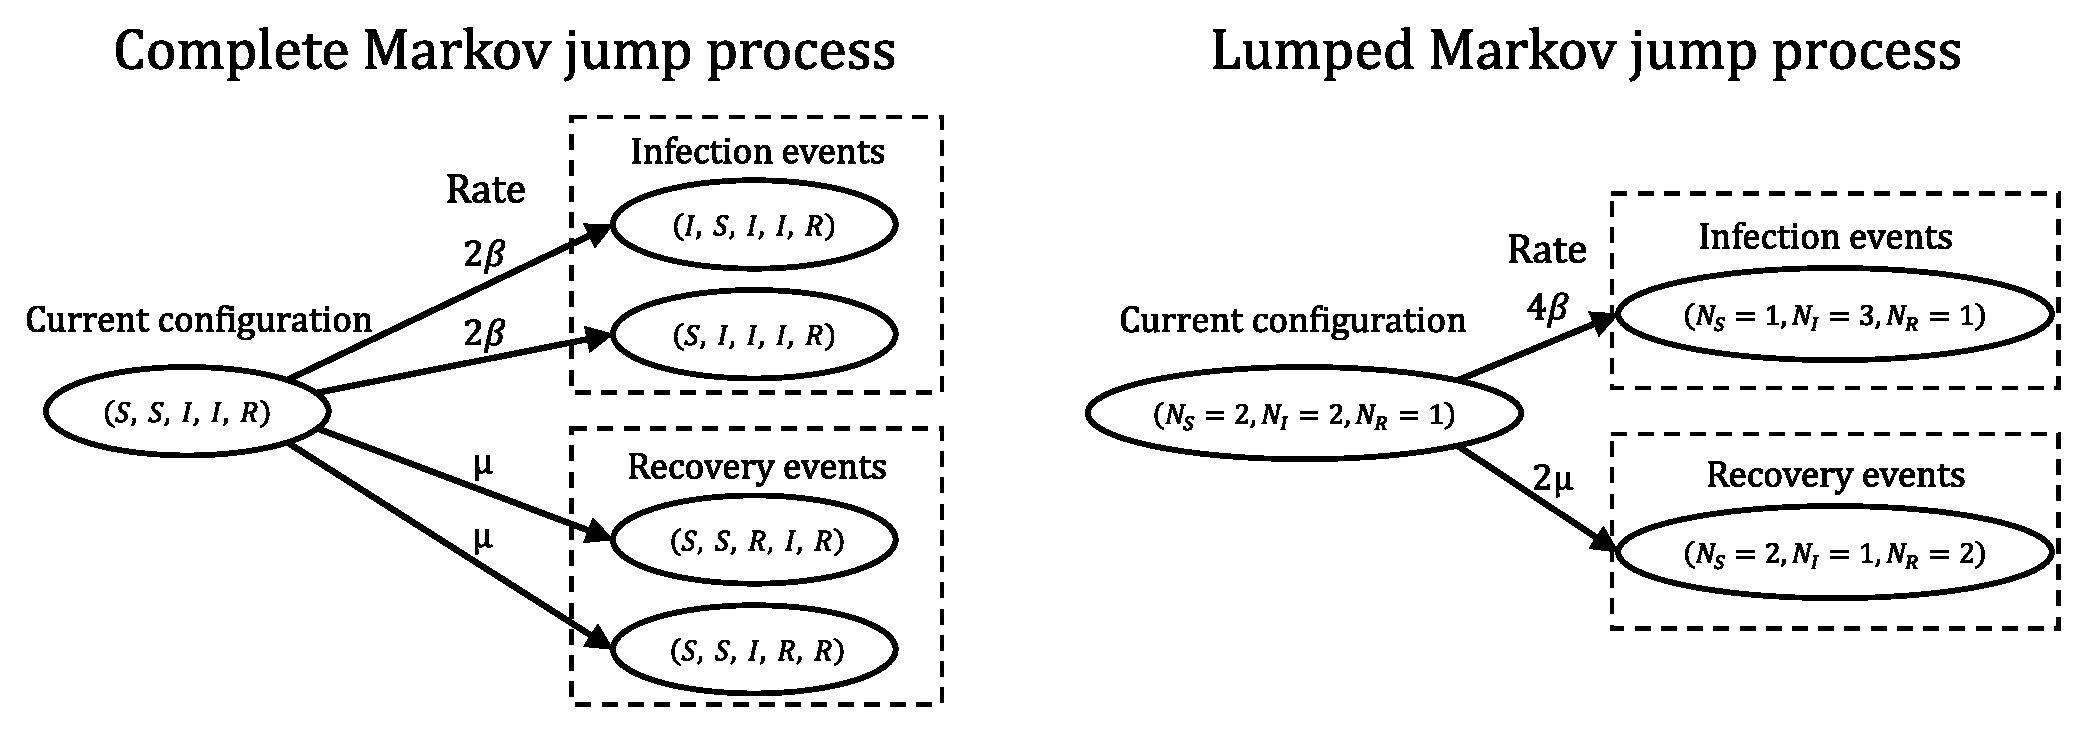
\includegraphics[width=\linewidth]{figures/SIR_representations}
	\caption[Individual and lumped representations of SIR dynamics.]{Complete and lumped representations of SIR dynamics in a population of five individuals. The per--contact infectivity rate, $ \beta $, and the recovery rate, $ \mu $, parameterize exponential waiting time distributions between transition events. The complete Markov jump process evolves on the state space of subject state labels, $ \mcS = \lbrace S,I,R\rbrace^N $, with dynamics determined by the subject--level transition rates. Each susceptible may contact two infected individuals, while each infected individual recovers independently. The lumped process evolves on the state space of compartment counts, $ \widebar{\mcS} = \lbrace N_S,N_I,N_R:\ N_S + N_I+N_R=N\rbrace $, with dynamics determined by lumped transition rates. The waiting time distributions between transitions are derived by noting that if $ \tau_1\sim \exp(\lambda_1) $ and $ \tau_2\sim\exp(\lambda_2) $, then $ \tau_{\min} = \min(\tau_1,\tau_2)\sim\exp(\lambda_1+\lambda_2) $.}
	\label{fig:sirrepresentations}
\end{figure}

Turning back to the SIR model, we defined the epidemic process, $ \bX(\tau) = (\bX_1,\dots,\bX_N)$, with state space $ \mcS = \lbrace S, I, R\rbrace^N $. Let $ \bx = (x_1,\dots,x_N) $ denote a configuration of the state labels (e.g. $ \bx = (S, I, S, R, I) $), and let $$ \overline{\bx} = h(\bx) = \left (l=\sum_{i=1}^N\ind{x_i = S},m=\sum_{i=1}^N\ind{x_i=I},n = \sum_{i=1}^N\ind{x_i=R}\right ) $$ be the corresponding vector of compartment counts. The lumped state space is 
$$ \overline{\mcS} = \left \lbrace \overline{\bx} = (l,m,n): l,m,n \in \lbrace0,\dots,N\rbrace,\  l+m+n = N \right \rbrace, $$ 
which partitions $ \mcS $ by summing the number of individuals in each disease state. 

The population--level SIR model expressed in terms of compartment counts, $ \overline{\bX} = (S, I, R) \in \overline{\mcS} $ (depicted in Figure \ref{fig:sirrepresentations}), evolves as a CTMC on the lumped state space $ \overline{\mcS} $ with transition rates
\begin{equation*}
\begin{array}{cc}
\underline{\text{Transition}} & \underline{\text{Lumped Rate}} \\
(S,I,R) \longrightarrow (S-1,I+1,R) & \beta S I ,\\
(S,I,R) \longrightarrow (S,I-1,R+1) & \mu I .
\end{array}
\end{equation*}
To see how we arrive at these rates, note that in a population with $ S $ susceptibles, each of whom is independently infected at rate $ \beta I $, the time until the first infection is exponentially distributed with rate $ \lambda_{SI} = \beta SI $ by the racing exponentials property (\ref{eqn:racing_exponentials}). Similarly, the time to the first recovery in a population with $ I $ infected individuals is exponentially distributed with rate $\lambda_{IR} = \mu I $. Note that the mean infectious period duration is still $ 1/\mu $, as it was in the case of the subject--level SIR model.

Again, let $ \btau = \lbrace\tau_0,\dots,\tau_{K+1}\rbrace $, be the (ordered) set of $ K $ infection and recovery times, along with the endpoints of the time period $ [\tau_0,\ \tau_{K+1}] $ over which the outbreak is modeled. We indicate by $ \ind{\tau_k \corresponds I} $ and $ \ind{\tau_k \corresponds R} $ whether $ \tau_k $ is an infection or recovery time, and let $ \btheta = (\beta, \mu, \overline{\bX}_0) $ denote the vector of parameters, including the initial state of $ \overline{\bX} $ at time $ \tau_0 $. The CTMC likelihood of $ \overline{\bX} $ over $ [\tau_0,\ \tau_{K+1}] $ is a product of exponential waiting time densities,
\begin{align} 
\label{eqn:sir_pop_likelihood}
L(\overline{\bX}| \btheta) &= \prod_{k = 1}^{K}\left \lbrace \left [\beta S_{\tau_k} I_{\tau_k}\times\ind{\tau_k \corresponds I} + \mu I_{\tau_k}\times\ind{\tau_k \corresponds R}\right ] \exp{\left [-\left (\tau_k - \tau_{k-1}\right )\left (\beta I_{\tau_k} S_{\tau_k} + \mu I_{\tau_k}\right )\right ]}\right \rbrace \nonumber \\
& \hspace{0.2in} \times \exp \left [-\left (t_L - \tau_K\right )\left (\beta I_{\tau_K^+}S_{\tau_K^+} + \mu I_{\tau_K^+}\right )\right ]. 
\end{align} 

\subsection{A Brief Review of CTMCs}
\label{subsec:ctmc_overview}

We briefly digress from our discussion of epidemic models to review some basic properties of CTMCs in a bit more generality. The following discussion is not intended to be comprehensive, but rather to provide an overview of some results that will be useful in this dissertation. We refer to \cite{bremaud1999markov,fuchs2013inference,guttorp1995stochastic,wilkinson2011stochastic} for more complete and rigorous discussions of the following material. For simplicity, we will focus on CTMCs with finite state spaces. 

The forward--time evolution of a CTMC is described by its transition kernel $$\Pr(\bX(\tau^\prime) = \bx^\prime | \bX(\tau) = \bx) = P_{\bx,\bx^\prime}(\tau,\tau^\prime),$$
where $ \bx,\bx^\prime\in\mcS $ and $ 0\leq\tau\leq\tau^\prime $. The transition kernel only depends on the time--elapsed when the process is time--homogeneous $ P_{\bx,\bx^\prime}(\tau,\tau^\prime) = P_{\bx,\bx^\prime}(|\tau^\prime - \tau|) \equiv P_{\bx,\bx^\prime}(\tau^\prime) $. In matrix form, the transition kernel, $ P $, is an $ r\times r $ stochastic matrix, where $ r = |\mcS| $, the rows of $ P $ sum to one, and $ P_{ii} = -\sum_{j\neq i}P_{ij}$. Trivially, $ P_{\bx,\bx^\prime}(0) = I $, i.e., there are no state changes in a time interval of zero length, almost surely. By the Markov property, the probability of transitioning from state $ i $ to state $ k $ in time $ s+t $ is 
\begin{equation}
\label{eqn:chapman_kolmogorov}
P_{ik}(s+t) = \sum_{j\in\mcS}P_{ij}(s)P_{jk}(t),
\end{equation}
or in matrix form, $$P(s+t) = P(s)P(t).$$
Equation (\ref{eqn:chapman_kolmogorov}) is known as the \textit{Chapman--Kolmogorov} master equation. 

The transition rate matrix (or \textit{infinitesimal generator}) of $ \bX $ is defined as the derivative of $ P(\tau) $ at $ \tau = 0 $, i.e.,
\begin{align*}
\label{eqn:ctmc_generator}
\bLambda &= \underset{\dtau \rightarrow 0}{\lim}\frac{P(\dtau) - P(0)}{\dtau} \\
&= \underset{\dtau \rightarrow 0}{\lim}\frac{P(\dtau) - I}{\dtau}, \\
\shortintertext{which implies that the infinitesimal transition matrix is} P(\dtau) &= I + \bLambda\dtau.
\end{align*}
Thus, for example, the infinitesimal transition probabilities for the population--level SIR model are
\begin{align*}
\Pr\left (\bX(\tau+\dtau) = (S-1, I+1, R) | \bX(\tau) = (S,I,R)\right ) &= \beta SI + o(\dtau), \\
\Pr\left (\bX(\tau+\dtau) = (S, I-1, R+1) | \bX(\tau) = (S,I,R)\right ) &= \mu I + o(\dtau).
\end{align*}
The transition probability matrix over an interval of arbitrary length, $ \tau $, solves the matrix differential equation,  \begin{equation}\label{eqn:kolmogorov_forward}
\deriv{}{\tau}P(\tau) = \bLambda P(\tau),\hspace{0.2in} s.t.\  P(0) = I.
\end{equation} 
Thus, $ P(\tau) = \exp(\bLambda\tau) $, can be computed using the matrix exponential. There are many ways to compute the matrix exponential \cite{moler2003nineteen}. We will typically do so by diagonalizing $ \bLambda $ and exponentiating the eigenvalues. Section \ref{sec:mtx_exp} outlines this procedure in two separate cases: when $ \bLambda$ has real--valued eigenvalues, and also when the eigenvalues are complex. Equation (\ref{eqn:kolmogorov_forward}) is known as the \textit{forward} Kolmogorov equation, and is obtained by computing the derivative
\begin{align*}
\deriv{}{\tau}P(\tau) &= \frac{P(\tau + \dtau) - P(\tau)}{\dtau} \\
&= \frac{P(\dtau)P(\tau) - P(\tau)}{\dtau} \\
&= \frac{P(\dtau) - I}{\dtau}P(\tau)\\
&= \bLambda P(\tau).
\end{align*}
The \textit{backward} Kolmogorov equation is similarly obtained by
\begin{align}
\deriv{}{\tau}P(\tau) &= \frac{P(\tau + \dtau) - P(\tau)}{\dtau} \nonumber \\
&= \frac{P(\tau)P(\dtau) - P(\tau)}{\dtau} \nonumber \\
&= P(\tau)\frac{P(\dtau) - I}{\dtau}\nonumber\\
&= P(\tau)\bLambda .
\end{align}

\subsection{Large Population Approximations}
\label{subsec:sem_approximations}

It is often infeasible to work with the CTMC formulation of a SEM when modeling an outbreak in a large population, particularly when working within a Bayesian MCMC framework. The cardinality of model's state space grows polynomially in the population size. This makes it difficult to efficiently sample from the posterior or to explore the likelihood surface, even when fitting SEMs with relatively simple dynamics. A second challenge is that as the population size grows, so too do the numbers of transition events. Hence, repeatedly evaluating the likelihoods (\ref{eqn:sir_subj_likelihood}) and (\ref{eqn:sir_pop_likelihood}) is prohibitively expensive. 

Two commonly used approximations of the MJP representation of a SEM are through a system of ordinary differential equations (ODEs) and through a system of stochastic differential equations (SDEs). We will not go into detail on the derivations of these representations, except to give some intuition about the conditions under which they are appropriate, and refer to \cite{allen2017primer,greenwood2009stochastic} for more detailed overviews. However, it is interesting to note that the Kolmogorov equations for the ODE, SDE, and MJP formulations of a SEM arise as special cases of a \textit{differential Chapman--Kolmogorov master equation} that generalizes (\ref{eqn:chapman_kolmogorov}) \cite{fuchs2013inference}. 

We presented the MJP representation of the SIR model as an \textit{extensive}, $ \bX $, where transition events led to jumps of size one in the compartment counts. We could have equivalently defined the model in terms of an \textit{intensive} process, $ \bXtil = \bX / N = (S/N,I/N,R/N) $, where transition events led to jumps of size $ 1/N $. As $ N\longrightarrow \infty$ , it becomes reasonable to consider approximating $ \bXtil $ by a process with continuous sample paths. The large population stochastic \textit{approximation} is the solution to an It\^{o} diffusion whose sample paths are continuous but nowhere differentiable. The infinite population deterministic functional \textit{limit} solves a system of ODEs and has smooth sample paths. We will present extensive forms of the SDE and ODE models, which are obtained by simply rescaling the intensive processes from which the approximations derive. 

\subsubsection{Deterministic representation as a system of ODEs}
\label{subsec:deterministic_models}

In the infinite population limit, sample paths of the SIR model are solutions to the following system of ODEs, subject to the initial constraint that $ \bX(\tau_0) = \bx_0 $:
\begin{align*}
\deriv{S}{t} = -\beta S I,\hspace{0.25in} 
\deriv{I}{t} = \beta S I - \mu I,\hspace{0.25in} 
\deriv{R}{t} = \mu I.
\end{align*}
The state space of the ODE representation of the SIR model is $$ \mcS^R =  \lbrace(j,k,l):\ j,k,l\in[0,N], j+k+l = N\rbrace. $$ Note that the ODE model implies that if $ I(\tau) > 0 $ at any time $ \tau $, then $ I(\tau) > 0\ \forall\ \tau\in[0,\infty)$. Therefore, the ODE model is not appropriate if we are interested in answering questions about the stochastic emergence or extinction of an outbreak.

ODE formulations of SEMs are particularly useful, in part, because they more easily lend themselves mathematical analysis. One important quantity that is straightforwardly derived for ODE models is the basic reproduction number, $ R_0 $, which is interpreted as the expected number of secondary infections attributable to a single index case in an otherwise susceptible population (of infinite size). The basic reproduction number can be related to both the final size distribution and to the probability of a major outbreak \cite{allen2017primer,greenwood2009stochastic,miller2012note}. Estimation of $ R_0 $ is more complicated for stochastic models, though it can be derived from a branching process approximation for the early behavior of an outbreak \cite{allen2008introduction}. In the case of deterministic models, $ R_0 $ is given by the spectral radius of the next generation matrix (NGM) for the linearized system of ODEs at the disease free equilibrium (DFE) \cite{diekmann2009construction,van2017reproduction}. Other methods exist, e.g., by analyzing the survival function or by fitting phenomenological models when the growth rate of the outbreak is observed to be subexponential \cite{van2017reproduction}.

As an example, we will demonstrate the NGM method for computing $ R_0 $ for an outbreak with SIR dynamics where a fraction of the population, $ p_v $, is vaccinated and vaccine efficacy (VE)  modifies the per--contact rate of infection (VE for susceptibility: $ \nu_s $), the infectiousness of carriers (VE for infectiousness: $ \nu_i $), and the rate of recovery (VE for recovery: $ \nu_r $). We will write $ N^{u} = (1-p_v)N $ and $ N^{v} = p_vN $. The DFE is \begin{small}
	$$ \bX_{DFE} =  (S^{(u)}_{DFE} = \left ((1 - p_v)N,\ I^{(u)}_{DFE} = 0,\  R^{(u)}_{DFE} = 0,\ S^{(v)}_{DFE} = p_vN,\ I^{(v)}_{DFE} = 0,\ R^{(v)}_{DFE} = 0)\right ). $$
\end{small} 
The linearized system of ODEs at the DFE is 
\begin{align*}
\deriv{I^{(u)}}{t} &= \beta \left (I^{(u)} + \nu_iI^{(v)}\right )N^{(u)} - \mu I^{(u)},\hspace{0.2in} 
\deriv{I^{(v)}}{t} = \beta \nu_s\left (I^{(u)} + \nu_iI^{(v)}\right )N^{(v)} - \mu\nu_r I^{(v)}.
\end{align*}	
The NGM is constructed as $K=-T\Sigma^{-1}$, where $T$ gives the rates of infectious contact between states at infection, $ I^{(u)} $ and $ I^{(v)} $, and $\Sigma$ contains the recovery rates out of states at infection. Here,
\begin{align*}
T &= \kbordermatrix{ & I^{(u)} & I^{(v)} \\
	I^{(u)} & \beta N^{u} & \nu_i\beta N^u\\
	I^{(v)} & \nu_s \beta N^{v} & \nu_s\nu_i\beta N^v}, & &\hspace{-2in}
\Sigma = \kbordermatrix{ & I^{(u)} & I^{(v)} \\
I^{(u)}&-\mu & 0 \\
I^{(v)}& 0 & -\mu\nu_r},\\
&\hspace{1.25in} K =\kbordermatrix{ & I^{(u)} & I^{(v)} \\
	I^{(u)} & \frac{\beta N^{u}}{\mu} & \frac{\nu_i\beta N^u}{\nu_r\mu}\\
	I^{(v)} & \frac{\nu_s \beta N^{v}}{\mu} & \frac{\nu_s\nu_i\beta N^v}{\nu_r\mu}}.
\end{align*}
Thus, $$ R_0 = \sigma(K) = \frac{1}{2}\left (Tr(K) + \sqrt{Tr(K)^2 - 4\det(K)}\right )  = \frac{\beta N^{u}}{\mu} + \frac{\nu_s\nu_i\beta N^v}{\nu_r\mu}.$$

\subsubsection{Diffusion approximations of Markov Jump Processes}
\label{subsubsec:diff_approx}

We will give the diffusion approximation for the SIR model after a, somewhat colloquial, review of diffusions based on material in \cite{fuchs2013inference,oksendal2003stochastic,schnoerr2017approximation,wilkinson2011stochastic}. We begin with the SDE \begin{equation}
\deriv{\bX_t}{t} = \bmu(\bX_t,t) + \bSigma(\bX_t,t)\bZ_t,\hspace{0.1in} t\geq s;\hspace{0.1in} \bX_x = \bx,\end{equation}
with \textit{drift vector} $ \bmu:\mathbb{R}^d\rightarrow\mathbb{R}^d $ and  \textit{diffusion matrix} $ \bSigma:\mathbb{R}^d\rightarrow \mathbb{R}^d\times\mathbb{R}^d $, which are interpretable as the infinitesimal first and second moments of the process innovations. $ \bZ_t $ is $ d $--dimensional Gaussian white noise. We denote by $ \rmd\bW_t = \bZ_t\dt$ standard $ d $--dimensional Brownian motion (see \cite{oksendal2003stochastic} for a formal definition). An \textit{It\^{o} diffusion} is a stochastic process, $ (\bX_t)_{t\geq0} $, that satisfies the It\^{o} stochastic integral equation
\begin{equation}
\bX_t = \bX_0 + \int_0^t\bmu(\bX_t,t)\dt + \int_0^t\bSigma(\bX_t,t)\rmd\bW_t,\end{equation}
which we can express equivalently in differential form,
\begin{equation}
\label{eqn:general_sde}
\rmd\bX_t = \bmu(\bX_t,t)\dt + \bSigma(\bX_t,t)\rmd\bW_t.
\end{equation}
The SDE (\ref{eqn:general_sde}) can be interpreted as the limit of a difference equation, $ \Delta\bX_t = \bmu(\bX_t,t)\Delta t + \bSigma(\bX_t,t)\Delta\bW_t $, with infinitely small time steps, $ \Delta t \rightarrow 0$. Hence, we can simulate approximate sample paths using an \textit{Euler--Maruyama} scheme by taking $ \Delta t = \epsilon>0 $ and sampling the innovations, $ \Delta\bX_t$, according to
$$\Delta\bX_t\sim MVN\left (\bmu(\bX_t,t)\Delta t,\ \bSigma(\bX_t,t)\bSigma(\bX_t,t)^T\Delta t\right ).$$

Given a $ d $--dimensional It\^{o} process of the form (\ref{eqn:general_sde}), \textit{It\^{o}'s lemma} gives a formula for the SDE satisfied by a transformed process \cite{oksendal2003stochastic}. Let $ g(\bx, t) = \left (g_1(\bx,t),\dots,g_p(\bx,t)\right ) $ be a twice continuously differentiable map from $ \mathbb{R}^d\times[0,\infty)\rightarrow\mathbb{R}^p $. Then the transformed process, $ \bY(\bW,t) = g(\bX_t, t)$, is also an It\^{o} process with component $ Y_k,\ k=1,\dots,p $, given by
$$\rmd Y_k, = \pdiv{g_k}{t}(\bX, t) + \sum_i\pdiv{g_k(\bX,t)}{x_i}\rmd X_i + \frac{1}{2}\sum_i\sum_j\pdiv{^2g_k(\bX,t)}{x_i\partial x_j}\rmd X_i\rmd X_j,$$
where $ \rmd W_i\rmd W_j = \dt\rmd W_i = \rmd W_i\dt = 0 $ and $ \rmd W_i\rmd W_i = \dt. $

The SDE approximation of a density dependent MJP can be rigorously derived in a number of ways. These include proving the convergence of the MJP Kolmogorov master equation to its SDE counterpart, convergence of the infinitesimal generator, and through a number of different system size expansions applied to the master equation \cite{fuchs2013inference}. An intuitive approach yielding an equivalent result, referred to as the \textit{Langevin approach}, postulates that the SDE approximation is obtained by matching the infinitesimal moments of the diffusion to those of the MJP \cite{fuchs2013inference,gillespie2000chemical,wallace2012linear}. 

We proceed by approximating the numbers of infections and recoveries in a small time interval, $ (t, t+\dt] $. Suppose that we can choose $ \dt $ so that the following \textit{leap} conditions hold:
\begin{enumerate}
	\item $ \dt $ is sufficiently \textit{small} that the $ \bX^c $ is essentially unchanged over $ (t,t+\dt] $, so that the rates of infections and recoveries are approximately constant: 
	\begin{equation}\label{eqn:tau_cond_1_background}
	\blambda(\bX^c(t^\prime)) \approx \blambda(\bx^c(t)),\ \forall t^\prime \in (t,t+\dt].
	\end{equation}
	\item $ \dt $ is sufficiently \textit{large} that we can expect many disease state transitions of each type:
	\begin{equation}\label{eqn:tau_cond_2_background}
	\blambda(\bx^c(t)) \gg \bs{1}.
	\end{equation}
\end{enumerate}
Condition (\ref{eqn:tau_cond_1_background}) can be trivially satisfied by choosing $ \dt $ to be infinitesimally small, and implies that the numbers of infections and recoveries in $ (t,t+\dt] $ are essentially independent of one another since the rates at which they occur are approximately constant within the interval \cite{gillespie2000chemical}. Furthermore, (\ref{eqn:tau_cond_1_background}) implies that the numbers of infections and recoveries in the interval are independent Poisson random variables with rates $ \blambda(\bx^c(t)\dt) $. For the SIR model, the numbers of infections and recoveries in an infinitesimal time increment are $ N_{SI}(\dt) \sim \mr{Poisson}(\beta S(t)I(t)\dt) $ and $ N_{IR}(t+\dt) \sim \mr{Poisson}(\mu I(t)\dt) $. Condition (\ref{eqn:tau_cond_2_background}), which we can reasonably expect to be satisfied in large populations where there are many infections and recoveries \cite{wallace2012linear}, implies that the Poisson distributed increments can be well approximated by independent Gaussian random variables. 

We now give the SDE approximation for the SIR model. Let $ \blambda(\bX) = (\lambda_{SI}, \lambda_{IR}) $ denote the rates at which individuals become infected and recover, and let $ \bA $ denote the matrix whose rows specify changes in counts of susceptible, infected, and recovered individuals corresponding to one infection or recovery event:
\begin{equation*}
\bA = \kbordermatrix{& S & I &  R\\
	S\rightarrow I& -1& 1 & 0\\
	I \rightarrow R & 0& -1 & 1
}.
\end{equation*}
The SDE for the SIR model is 
\begin{equation}
\label{eqn:sir_sde}
\rmd\bX(t) = \bA^T\blambda(\bX)\dt + \sqrt{\bA^T\diag(\blambda(\bX))\bA}\rmd\bW_t.
\end{equation}
This SDE is referred to as the \textit{chemical Langevin equation} (CLE). If we wanted to change the model dynamics, the expressions for $ \bA $ and $ \blambda $ would differ, but the diffusion approximation would be of the same form (with the caveat that $ \blambda $ must satisfy certain Lipschitz conditions to ensure existence of the SDE, see \cite{fuchs2013inference,oksendal2003stochastic}). 

\subsubsection{Linear Noise Approximation}
\label{subsubsec:lna_background}

The intractability of the CLE transition density is problematic when using the CLE as a basis for inference. Absent additional simplifying assumptions, e.g., as in \cite{cauchemez2008}, inference with SDEs typically relies on simulation based methods, e.g., \cite{dukic2012,golightly2013simulation,golightly2018efficient}. An attractive alternative, dating to at least the 1970s \cite{kurtz1970solutions,kurtz1971limit}, but that has received attention in recent years, involves approximating the CLE by a Gaussian state space model, the moments of which are solutions to systems of ODEs that are related to the transition rates of the MJP and its SDE approximation. This approximation is known as the \textit{linear noise approximation} (LNA) and it will be the methodological basis for Chapters \ref{chap:lna_for_sems} and \ref{chap:lna_extensions} of this dissertation. Our informal derivation of the LNA follows \cite{golightly2013simulation,wilkinson2011stochastic}. Rigorous derivations can be found in \cite{elf2003fast,kurtz1981approximation,vankampen2007stochastic,wallace2012linear}. 

We take the SDE (\ref{eqn:sir_sde}) as our starting point and express the transition rates in terms of intensive concentrations. Letting $ \bXtil \equiv \bXtil(t) = \bX(t)/N $ and suppressing the dependence on $ \btheta $, we have $  \blambda(\bX) = N\lambda(\bXtil) $. The rescaled CLE is 
\begin{align}
\rmd \bX_t &= N\bA^T\blambda(\bXtil_t)\dt + \sqrt{N\bA^T\diag(\blambda(\bXtil_t))\bA}\rmd\bW_t \nonumber\\
\label{eqn:cle_conc}
\implies \rmd\bXtil_t &= \bA^T\blambda(\bXtil_t)\dt + \frac{1}{\sqrt{N}}\sqrt{\bA^T\diag(\blambda(\bXtil_t))\bA}\rmd\bW_t.
\end{align}
In the infinite population limit, the stochastic contribution to this SDE is negligible and we obtain the deterministic ODE limit of the intensive process, $ \boetatil $, which solves the ODE,
\begin{equation}
\label{eqn:lna_drift}
\deriv{\boetatil(t)}{t} = \bA^T\blambda(\boetatil(t)),\hspace{0.2in} \boetatil(t_0)=\boetatil_0.
\end{equation}
When stochasticity not negligible and the population size is large, i.e., when we think the leap conditions (\ref{eqn:tau_cond_1_background}) and (\ref{eqn:tau_cond_2_background}) are satisfied, we might reasonably expect $ \bX_t $ to behave like its deterministic limit plus residual Poisson variation. Thus, we decompose
\begin{equation}
\label{eqn:lna_ansatz}
\bX_t = N\boetatil_t + \sqrt{N}\bMtil_t,
\end{equation}
 i.e., $ \bMtil_t = \sqrt{N}(\bXtil_t - \boetatil_t) $, and assume $ ||\bXtil_t - \boetatil_t|| = \mcO(N^{-1/2}) $. Substituting (\ref{eqn:lna_ansatz}) into (\ref{eqn:cle_conc}),
 \begin{equation}
 \label{eqn:cle_conc_sub}
 \rmd\boetatil_t + \frac{1}{\sqrt{N}}\rmd\bMtil_t = \bA^T\blambda\left (\boetatil_t + \frac{1}{\sqrt{N}}\bMtil_t\right )\dt + \frac{1}{\sqrt{N}}\sqrt{\bA^T\diag\left (\blambda\left (\boetatil_t + \frac{1}{\sqrt{N}}\bMtil_t\right )\right )\bA}\rmd\bW_t. 
 \end{equation}
Taylor expanding $ \blambda\left (\boetatil_t + \frac{1}{\sqrt{N}}\bMtil_t\right ) $ about $ \boetatil_t $, and collecting terms of order $ \mcO(N^{-1}) $ and higher, gives $$\blambda\left (\boetatil_t + \frac{1}{\sqrt{N}}\bMtil_t\right ) = \blambda\left (\boetatil_t\right ) + \frac{1}{\sqrt{N}}\bFtil_t\bMtil_t + \mcO(N^{-1}),$$
where $ \bFtil $ is the Jacobian of $ \blambda(\cdot) $ evaluated at $ \boetatil_t $. We substitute \ref{eqn:cle_conc_sub} and again discard terms of order $ \mcO(N^{-1}) $,
\begin{align}
\rmd\boetatil_t + \frac{1}{\sqrt{N}}\rmd\bMtil_t &\approx \bA^T\left (\blambda\left (\boetatil_t\right ) + \frac{1}{\sqrt{N}}\bFtil_t\bMtil_t\right )\dt \nonumber \\
&\hspace{0.5in} +\frac{1}{\sqrt{N}}\sqrt{\bA^T\diag\left (\blambda\left (\boetatil_t\right ) + \frac{1}{\sqrt{N}}\bFtil_t\bMtil_t\right )\bA}\rmd\bW_t \nonumber \\
&= \bA^T\left (\blambda\left (\boetatil_t\right ) + \frac{1}{\sqrt{N}}\bFtil_t\bMtil_t\right )\dt + \frac{1}{\sqrt{N}}\sqrt{\bA^T\diag\left (\blambda\left (\boetatil_t\right )\right )\bA}\rmd\bW_t + \mcO(N^{-1}) \nonumber\\
&= \rmd\boetatil_t  + \frac{1}{\sqrt{N}}\bA^T\bFtil_t\bMtil_t\dt + \frac{1}{\sqrt{N}}\sqrt{\bA^T\diag(\blambda(\boetatil_t))\bA}\rmd\bW_t,\nonumber
\end{align}
where the last equation follows from (\ref{eqn:lna_drift}). Hence,
\begin{align}
\label{eqn:lna_sde}
\rmd\bMtil_t &= \bA^T\bFtil_t\bMtil_t\dt + \sqrt{\bA^T\diag\left (\blambda(\boetatil_t)\right )\bA}\rmd\bW_t.
\end{align}
This final equation is the LNA; it is a linear SDE for the residual process in the decomposition (\ref{eqn:lna_ansatz}). Therefore, the CLE (\ref{eqn:cle_conc}) is approximated by the sum of a non--linear deterministic ODE for its drift, and a linear SDE for the residual variability. 

The SDE (\ref{eqn:lna_sde}) for the residual process is linear in $ \bMtil_t $ with time--inhomogeneous drift and diffusion. For fixed or Gaussian initial conditions, $ \bMtil_0 = \bmtil_0 $, the distribution of $ \bMtil_t|\bmtil(t_0),\ t\geq t_0 $ is Gaussian,
\begin{equation}
\label{eqn:lna_resid_dist}
\bMtil_t|\bmtil(t_0) \sim MVN(\bmu_t,\bSigma_t),
\end{equation}
and the moments of (\ref{eqn:lna_resid_dist}) are obtained by solving the coupled ODEs,
\begin{align}
\label{eqn:lna_drift_gen}
\deriv{\boetatil_t}{t} &= \bA^T\blambda(\boetatil_t), & \boetatil(t_0) = \boetatil_0,\\
\label{eqn:lna_resid_gen}
\deriv{\bmu_t}{t} &= \bA^T\bFtil_t\bmu_t, & \bmu(t_0) = \bmtil_0, \\
\label{eqn:lna_diff_gen}
\deriv{\bSigma_t}{t} &= \bA\bFtil_t\bSigma_t + \bA^T\diag(\blambda(\boetatil_t))\bA + \bSigma_t\bFtil_t^T\bA^T, & \bSigma(t_0) = \bsigma_0. 
\end{align}
Hence,
\begin{equation}
\bXtil_t|\bxtil(t_0) \sim MVN(\boetatil_t + \bmu_t,\bSigma_t).
\end{equation}
Note that we have suppressed the dependence of $ \bFtil $ and $ \bSigma $ on $ \boetatil $ for clarity. Derivations of the LNA solution may be found in \cite{vankampen2007stochastic,wallace2012linear,whitaker2016bayesian}. In general, the LNA ODEs (\ref{eqn:lna_drift_gen}), (\ref{eqn:lna_resid_gen}), and (\ref{eqn:lna_diff_gen}), need to be solved numerically. 

\subsection{Inference and Computation for Stochastic Epidemic Models}
\label{subsec:sem_exact_inf}
Inference for SEMs based on CTMC representations of the epidemic process has historically relied on four, not mutually exclusive, classes of methods \cite{oneill2010}: martingale methods, simulation--based methods, data augmentation, and approximation of the CTMC. 

Martingale methods estimate the parameters of interest using estimating equations based on martingales for counting processes embedded within the SEM, e.g., for infections and recoveries \citep{andersson2000stochastic,becker1977general,lau2008estimating, lindenstrand2013estimation,sudbury1985proportion}. However, these methods are not easily implemented for SEMs with complex dynamics fit to partially observed count data.

Simulation based methods use the SEM to generate latent epidemic paths that serve as the basis for inference. This class of methods includes approximate Bayesian computation (ABC) methods \citep{mckinley2009,toni2009,mckinley2018approximate}, pseudo--marginal methods \citep{mckinley2014simulation,shubin2016revealing}, and sequential Monte Carlo (or particle filter) methods \cite{andrieu2010particle, dukic2012,golightly2018efficient,ionides2011iterated,koepke2016predictive,toni2009}. Within this class, the particle marginal Metropolis--Hastings (PMMH) algorithm of \cite{andrieu2010particle} stands out as a general method for Bayesian inference and is used as a benchmark method in Chapter \ref{chap:bda_for_fitting_sems_to_prevalence_data}. Although simulation--based methods have been used to fit complex models, the computational cost of simulating from CTMCs can become prohibitive for complex models. Furthermore, simulation--based methods suffer from well known pitfalls. ABC methods are sensitive to the choice of summary statistic, rejection threshold, and prior  \cite{toni2009}. Sequential Monte Carlo methods, on which pseudo--marginal methods often rely, are prone to ``particle impoverishment" problems \cite{cappe2006inference, dukic2012}. Examples of particle degeneracy are presented in supplementary Chapter \ref{chap:appendix_ch3}, and an inability to fit models  with complex dynamics with reasonable effort led us to abandon PMMH as a benchmark for the more complex models in Chapters \ref{chap:lna_for_sems} and \ref{chap:lna_extensions}. 

Approximation methods replace the CTMC representation of a SEM with a model whose likelihood is more tractable. A common simplification is to discretize time and to construct a transition model for the population flow between model compartments over discrete time intervals. Discrete time SEMs are often derived from chain--binomial models where, most commonly, a binomially distributed subset of the susceptible population becomes infected over each time step. The most famous examples are the Greenwood model \cite{greenwood1931statistical}, where the number of newly infected individuals is directly modeled as a binomial sample of the susceptible population, and the Reed--Frost epidemic model \cite{abbey1952examination}, where binomially distributed incidence is depends on the probability that each susceptible escapes infection. Typically, infected individuals are assumed to recover in a fixed number of time steps. It is also possible to construct models with more general dynamics, for example, by allowing for latent periods or random infectious period durations, \cite{lekone2006}. When the probability of infection is low, it is possible to approximate binomial counts using Poisson or negative binomial distributions \cite{held2005,paul2011predictive}. A related class of discrete time models, referred to as time series susceptible--infected--recovered (TSIR) models, derives conditionally Poisson or negative binomial incidence distributions from birth--death processes \cite{bjornstad2002dynamics,finkenstadt2000time,finkenstadt2002stochastic,glass2003}. An overview of discrete time epidemic models is given in \cite{wakefield2017spatio}.

Discrete time SEMs are attractive due to their relatively low computational cost. This is particularly true when it is reasonable to assume that underreporting is negligible (and hence ignored) since the observed data likelihood decomposes into products of standard probability distributions and thus requires little in the way of specialized machinery for MCMC or likelihood based methods. Further approximation by Poissons or negative binomials provides even more computational advantage, even when the dynamics are temporally or spatially complicated   \cite{bauer2016bayesian,held2005,fisher2017time,meyer2017incorporating}. In settings where incidence is under--reported, it may be reasonable to estimate an inflation factor for the observed count \cite{finkenstadt2000time,wakefield2017spatio}. Another approach is to integrate over the true incidence using sequential Monte Carlo or particle filter methods \cite{dukic2012,ionides2006inference,ionides2011iterated,shubin2016revealing}. However, as previously discussed, simulation--based methods can quickly become impractical for complex models. 

Among continuous--time approximations, the ODE and SDE representations are, arguably, the most common. ODE models are typically quite easy to work with from a computational standpoint, and MCMC can proceed in a relatively straightforward manner without relying on specialized machinery. Inference based on the SDEs typically relies on either simulation--based computational tools, as discussed in the previous paragraph, or further simplification of the SEM. For example, \cite{cauchemez2004bayesian,cauchemez2008,roberts2001} use diffusion processes that approximate the SEM dynamics, while \cite{jandarov2014} use a Gaussian process approximation of a related gravity model. As is the case for any approximation, the price of improved computational efficiency and tractability is that simplifying assumptions used in the various approximations must be justified. For instance, the diffusion approximation may not be valid in small populations where the system is far from its deterministic limit (and in which case we should be even more skeptical of the validity of the ODE approximation) \cite{andersson2000stochastic}.

The LNA has been a fixture in the literature on biochemical reaction networks since at least the 1970s when it appeared in a series of papers on approximations of density dependent Markov jump processes \cite{kurtz1970solutions,kurtz1971limit}. The LNA has been broadly applied in the analysis of gene regulatory networks, e.g., \cite{finkenstadt2013quantifying,giagos2010inference,hey2015stochastic,komorowski2009,stathopoulos2013markov,thomas2012slow,zimmer2015deterministic}. A review of the LNA, along with related approximations that derive from various system size expansions of the MJP Kolmogorov forward equation, can be found in \cite{schnoerr2017approximation,wallace2012linear}. The LNA has recently found applications in outbreak modeling in \cite{black2010stochastic,fearnhead2014,golightly2015delayed,golightly2018bridge,ross2009parameter,ross2012parameter,rebuli2017hybrid,zimmer2017likelihood}. To our knowledge, all applications of the LNA to outbreak modeling have assumed that the prevalence or cumulative incidence is normally distributed, or has used simulation based methods to incorporate non--Gaussian emission distributions into the model. We regard both of these constraints on the emission distribution as limitations. Comparison of the LNA with other moment--closure approximations in \cite{grima2012study} and \cite{buckingham2018gaussian}, who benchmarked the LNA in the context of the SIR model. In this dissertation, we will use the a restarting version of the LNA where the ODEs of the LNA transition density are restarted as data accumulates. Resetting the LNA ODEs has been established to improve accuracy over long time intervals \cite{fearnhead2014,folia2017trajectory,giagos2010inference}.

Finally, agent--based data augmentation (DA) methods for fitting SEMs, first presented in \cite{gibson1998,oneill1999}, target the joint posterior distribution of the missing data and model parameters to obtain a tractable complete data likelihood. That the augmentation is agent--based refers to the introduction of subject--level disease histories, rather than population--level epidemic paths, as latent variables in the model. An advantage of the agent--based approach is that household structure and subject--level covariates may be incorporated into the model \cite{auranen2000,hohle2002,cauchemez2004bayesian, neal2004statistical,oneill2009}. Development of DA methods for SEMs is of continuing interest, both in settings where the data consist of aggregate counts \cite{pooley2015,QinShe15,shestopaloff2016sampling}, and when the data reflect subject--level transition events \cite{kypraios2018bayesian,xu2016bayesian}.

\section{Bayesian Computation and Markov Chain Monte Carlo}
\label{sec:bayesian_computation}

The objective of Bayesian inference is to quantify uncertainty about a parameter of interest, $ \theta $, given data, $ y $. Uncertainty in the Bayesian paradigm is quantified through the posterior distribution, $$\pi(\theta|y)=\frac{\pi(y|\theta)\pi(\theta)}{\pi(y)},$$
where $ \pi(y|\theta) $ and $ \pi(\theta) $ are the sampling distribution and the prior distribution. The marginal distribution of the data, $ \pi(y) = \int\pi(y|\theta)\rmd\theta $, is constant with respect to $ \theta $, and so we typically work with the unnormalized posterior, $$ \pi(\theta|y)\propto\pi(y|\theta)\pi(\theta). $$

Having computed a posterior, we define a Bayes estimator as a decision rule that minimizes the expected posterior loss, or Bayes risk, $ \E_{\theta|y}(L(\theta,\thetahat)) $, i.e., $$ \widehat{\theta} = \underset{\theta^\prime}{\mr{argmin}}\int L(\theta,\theta^\prime(y)) \pi(\theta|y)\rmd\theta .$$ Some common Bayes estimators are the posterior mean, which minimizes the expected squared error loss, and the posterior median, which minimizes expected absolute error. More broadly, we are interested in the posterior distribution of a function, $ f(\theta) $,  $$\E_{\theta|y}(f(\theta)) = \int f(\theta)\pi(\theta|y)\rmd\theta.$$
This integral is frequently intractable. However, we can approximate it numerically by Monte Carlo integration. Suppose $ \theta_i\overset{i.i.d.}{\sim}\pi(\theta|y) $ and $ \E_{\theta|y}(f(\theta))<\infty $. Then, by the strong law of large numbers (SLLN), 
\begin{align*}
\what{\mu}_n &= \frac{1}{n}\sum_{i=1}^n f(\theta_i) \overset{a.s.}{\longrightarrow} E_{\theta|y}(f(\theta)),\ \hspace{0.1in} n\longrightarrow\infty\\
\what{\sigma}^2_n &= \frac{1}{n}\sum_{i=1}^n (f(\theta_i) - \what{\mu}_n)^2 \overset{a.s.}{\longrightarrow}\Var_{\theta|y}(f(\theta)).
\end{align*}
Hence, we approximate $ \E_{\theta|y}(f(\theta)) $ by the Monte Carlo estimate, $ \what{\mu}_n $. The distribution of the ordinary Monte Carlo estimate is given to us by the central limit theorem (CLT), 
$$\frac{\what{\mu}_n - \E_{\theta|y}(f(\theta))}{\what{\sigma}_n/\sqrt{n}}\overset{\mcL}{\longrightarrow}Z\sim N(0,1),$$
as $ \Var(\what{\mu}_n) \approx \Var\left (\frac{1}{n}\sum_{i=1}^n f(\theta_i)\right ) = \frac{1}{n^2}\sum_{i=1}^n\Var(f(\theta_i)) \implies\Var(\what{\mu}_n) =\what{\sigma}_n^2 / n. $ The quantity, $ \what{\sigma}_n/n $, is called the Monte Carlo standard error (MCSE).  

\subsection{Markov Chain Monte Carlo}
\label{subsec:mcmc}

MCMC is a framework for numerical integration that can be used to obtain an approximate sample from a posterior that we cannot evaluate analytically and from which it is not possible to sample directly via ordinary Monte Carlo. The strategy is to construct an ergodic (aperiodic and irreducible) Markov chain, $ \lbrace \theta_n\rbrace $, whose stationary distribution is $ \pi(\theta|y) $. The transition kernel of a Markov chain, $ K(\theta,\theta^\prime) $, gives the probability of moving from $ \theta $ to $ \theta^\prime $, which are elements in the support of the stationary distribution. The Markov chain preserves the stationary distribution if it satisfies the global balance condition,
$$\pi(\theta) = \int K(\theta^\prime,\theta)\pi(\theta^\prime)\rmd \theta^\prime.$$
It is typically difficult to directly confirm that a transition kernel satisfies global balance. Fortunately, we verify global balance by proving that the kernel satisfies a stronger condition called detailed balance,
$$\pi(\theta)K(\theta^\prime,\theta) = \pi(\theta^\prime)K(\theta,\theta^\prime),\ \forall \theta,\theta^\prime.$$

Though samples drawn from the Markov chain are correlated, the ergodic theorem ensures that the ergodic mean of an integrable function will converge, almost surely, to its target, i.e.,
$$\lim\limits_{n\longrightarrow\infty}\sum_{i=1}^n\E_{\theta|y}(f(\theta_i)).$$
Due to the autocorrelation of MCMC samples, the estimated Monte Carlo variance is now 
$$\what{\sigma}_n^2 = \frac{1}{n}\frac{1}{\what{n}_{eff}}\sum_{i=1}^n(f(\theta_i) - \what{\mu}_n)^2,$$
where $ \what{n}_{eff} = n / \left (1 + 2\sum_{\ell=1}^{\infty}\what{\rho}(\ell)\right ) $, and $ \what{\rho}(\ell) $ is the estimated autocorrelation at lag $ \ell $. 

It is often challenging to design an MCMC scheme that explores the posterior efficiently. The theory of MCMC merely guarantees that samples from a Markov chain will approximate the target posterior if we run it long enough. In practice, the choice of MCMC transition kernel, along with the model parameterization, are critically important to the computational efficiency of the MCMC and, moreover, to the validity of the MCMC sample as an approximation to the posterior \cite{betancourt2017conceptual}. We now present several MCMC algorithms that will be used throughout this dissertation. 

\subsubsection{Metropolis--Hastings Sampler}
\label{subsubsec:metropolis_hastings}

One of the most important MCMC sampler, due to its simplicity and generality, is the Metropolis--Hastings (MH) algorithm \cite{hastings1970monte,metropolis1953equation}. At each step in the Markov chain, a new state is proposed from the distribution $ q(\prop{\theta}|\cur{\theta}) $, and is accepted with probability
\begin{align}
\label{eqn:metropolis_hastings_1}
\alpha_{\cur{\theta}\rightarrow\prop{\theta}} &= \min\left \lbrace 1, \frac{\pi(\prop{\theta}|y)}{\pi(\cur{\theta}|y)}\frac{q(\cur{\theta}|\prop{\theta})}{q(\prop{\theta}|\cur{\theta})}\right \rbrace \\
\label{eqn:metropolis_hastings_2}
&= \min\left \lbrace 1, \frac{\pi(y|\prop{\theta})\pi(\prop{\theta})}{\pi(y|\cur{\theta})\pi(\cur{\theta})}\frac{q(\cur{\theta}|\prop{\theta})}{q(\prop{\theta}|\cur{\theta})}\right \rbrace.
\end{align}
The Metropolis--Hastings acceptance ratio has a nice interpretation as the ratio of posteriors for the proposed and current state, multiplied by the ratio of proposal probabilities for the reverse and forward transitions. When the next value is proposed from a symmetric distribution centered at the current state, the proposal densities cancel out and the algorithm is referred to as the Metropolis algorithm (this was the original formulation given in \cite{metropolis1953equation}). The proposal distribution Metropolis algorithm is typically a multivariate Gaussian.

The computational efficiency of the MH algorithm depends on having a proposal distribution that proposes jumps that are not so large as to never be accepted, but large enough that the sampler is able to explore the parameter space reasonably quickly. One strategy for achieving good performance is to obtain an empirical estimate of the posterior covariance matrix, which is then rescaled by a theoretically optimal factor \cite{,gelman1997weak,roberts2001optimal,roberts2009examples}. Alternately, the proposal covariance can be estimated adaptively over the MCMC run and tuned to achieve a target acceptance rate for proposals \cite{andrieu2008tutorial,liang2011advanced}. 

\begin{algorithm}[htbp]
	\caption{Metropolis--Hastings sampler.}
	\label{alg:metropolis_hastings}
	\begin{algorithmic}[1]
		\Procedure{MetropolisHastings}{$ \cur{\theta} $}
		\State Propose new value: $ \prop{\theta} \sim q(\prop{\theta}|\cur{\theta}) $
		\State Compute MH acceptance probability: $ \alpha = \min\left \lbrace 1, \frac{\pi(\prop{\theta}|y)}{\pi(\cur{\theta}|y)}\frac{q(\cur{\theta}|\prop{\theta})}{q(\prop{\theta}|\cur{\theta})}\right \rbrace $
		\State Sample $ u\sim Unif(0,1) $
		\State Accept/reject proposal: \vspace{-0.1in}
			\begin{equation*}
			\new{\theta} = \left\lbrace \begin{array}{ll}
			\prop{\theta},&\ \text{if}\ \alpha \geq u,\\
			\cur{\theta},&\ \text{if}\ \alpha < u.
			\end{array} \right.
			\end{equation*}
		\EndProcedure
	\end{algorithmic}
\end{algorithm}

\subsubsection{Gibbs Sampler}
\label{subsubsec:gibbs}

The Gibbs sampler \cite{geman1984stochastic} arises as a special case of MH when we update a parameter, from its full conditional distribution, $ \pi(\theta_j|\btheta_{-j},y) $, given the values of other parameters. MCMC samples obtained from single--site Gibbs updates can become strongly autocorrelated, resulting in poor MCMC mixing. One solution is to jointly update blocks of model parameters from their full conditionals, $ \pi(\btheta_{J}|\btheta_{-J},y) $, ideally grouping together parameters that are strongly correlated and minimizing the correlation between blocks \cite{knorr2002block,roberts1997updating,rue2005gaussian}.

The MH acceptance probability for the Gibbs sampler is one, thus all Gibbs proposals are automatically accepted. To see why this is so, note that $$q(\btheta_{J}|\btheta_{-J},y) = \frac{\pi(\btheta|y)}{\pi(\btheta_{-J}|y)} \propto\pi(\btheta|y).$$
Therefore, the MH ratio simplifies as
\begin{align*}
\frac{\pi(\prop{\btheta_J},\cur{\btheta_{-J}}|y)}{\pi(\cur{\btheta_J},\cur{\btheta_{-J}}|y)}\frac{q(\cur{\btheta_J}|\prop{\btheta_{-J}},y)}{q(\prop{\btheta_J}|\cur{\btheta_{-J}},y)} &= \frac{\pi(\prop{\btheta_J},\cur{\btheta_{-J}}|y)}{\pi(\cur{\btheta_J},\cur{\btheta_{-J}}|y)}\frac{\pi(\cur{\btheta_J},\cur{\btheta_{-J}}|y)}{\pi(\prop{\btheta_J},\cur{\btheta_{-J}}|y)}\frac{\pi(\btheta_{-J}|y)}{\pi(\btheta_{-J}|y)} = 1. \\
\end{align*}
Hence, an attractive property of the Gibbs sampler is that there are no tuning parameters that need to be optimized. This lends some robustness to the algorithm from a user standpoint.  

\begin{algorithm}[htbp]
	\caption{Gibbs sampler.}
	\label{alg:gibbs}
	\begin{algorithmic}[1]
		\Procedure{Gibbs}{$ \cur{\theta},\ \mcI = \lbrace J_1,\dots,J_p\rbrace $ parameter/block indices.}
		\For{$ J\in1,\dots,p $}
			\State Update: $ \theta_{J_i}|\theta_{-J_i},y\sim\pi(\theta_{J_i}|\theta_{-J_i},y) $
		\EndFor
		\EndProcedure
	\end{algorithmic}
\end{algorithm}

\subsubsection{Slice sampling}
\label{subsubsec:slice_sampling}

Slice sampling methods are a class of auxiliary variable MCMC methods predicated on the idea that sampling from a density proportional to a function, $ \pi(\btheta)\propto f(\btheta) \in \bbR^n $, is equivalent to sampling uniformly from the $ n+1 $ dimensional volume beneath $ f(\btheta) $. These methods occupy an attractive middle ground between simple algorithms that lazily explore the parameter space and may suffer from convergence and mixing issues (e.g., random walk Metropolis--Hastings), and complex gradient based methods that effectively suppress random walks but may be prohibitively expensive due to the need for repeated evaluation of likelihood gradients within each MCMC iteration (e.g., Hamiltonian Monte Carlo). Slice sampling methods have been shown to have attractive robustness properties are able to suppress random walk behavior that results in high dimensional problems \cite{mira2002efficiency,roberts1999convergence,neal2003slice}. Moreover, slice samplers are flexible and easily implemented for a broad class of computational problems. Hence, slice samplers will often be our method of choice for fitting complex SEMs. 

We introduce slice sampling by considering the task of sampling a random variable, $ \theta\in\bbR $ with density $ \pi(\theta)\propto f(\theta) $.  Rather than sample $ \theta $ directly, we introduce an auxiliary variable, $ u $, defined such that the joint density of $ (\theta,u) $ is uniform over the area $ S = \lbrace (\theta,u):\ 0<u<f(\theta) \rbrace. $ Slice sampling alternates Gibbs updates of $ \theta|u $ and $ u|\theta $ from their full conditionals,
\begin{align*}
\pi(u|\theta) &\sim Unif(0,f(\theta)) \\
\pi(\theta|u) &\sim \mathrm{Unif}(\mcS),\ S = \lbrace \theta: f(\theta) > u\rbrace.
\end{align*}
In the case of slice sampling $ \theta $ from its posterior, $ \pi(\theta|y)\propto f(\theta) \equiv L(y|\theta)\pi(\theta) $. The algorithm is otherwise unchanged. 

\begin{algorithm}[htbp]
	\caption{Univariate slice sampling intuition.}\label{alg:univar_slice_intuition}
	\begin{algorithmic}[1]
		\Procedure{SliceSampler}{$ \cur{\theta},\cur{u} $}
		\State Vertical update: $ \new{u}|\cur{\theta} \sim \mathrm{Unif}(0,f(\theta))$,
		\State Horizontal update: $ \new{\theta}|\new{u} \sim \mathrm{Unif}(S),\ S = \lbrace \theta: f(\theta) > \new{u}\rbrace$.
		\EndProcedure
	\end{algorithmic}
\end{algorithm}

Sampling $ u|\theta $ is trivial. However, we often lack an analytical expression for the slice corresponding to $ \theta|u $. In principal, an approximate interval, $ S^\prime $ need not contain all of $ S $. However, if $ S' $ is too small, the Markov chain will be unable to make big moves, resulting in highly autocorrelated posterior samples. In contrast, too large a bracket will result in many rejections, and hence many unnecessary likelihood evaluations. Several possibilities for approximating $ S $ are listed in \cite{neal2003slice}. The key condition that must be satisfied in any interval selection procedure in order for the Markov chain to satisfy detailed balance is that $ \Pr(S'|\cur{\theta}) = \Pr(S'|\new{\theta}) $. Hence, the set of valid proposals, $ A $, is the set of points for which the probability of selecting an approximate bracket, $ S^\prime $, is equal to the probability of selecting $ S^\prime $ from current state, i.e., \[ A = \lbrace \theta': \theta' \in S\cap S',\ \mathrm{and}\ \Pr(S'|\theta) = \Pr(S'|\theta')\rbrace. \]

Given the current state $ \theta $, threshold $ u $, and initial bracket width $ \omega $, we can ``step out" to expand the interval until it covers $ S $. If the resulting interval is too wide, we can shrink the corresponding bracket endpoint to the rejected value and propose a new value uniformly within the new bracket. We will typically tune the initial bracket width throughout the MCMC run to encourage an equal number of bracket expansions to shrinkages, which minimizes the expected number of likelihood evaluations per MCMC iteration \cite{tibbits2014automated}.

\begin{algorithm}[htbp]
	\caption{Univariate slice sampling with stepping out.}\label{alg:univar_slice}
	\begin{algorithmic}[1]
		\Procedure{SliceSampler1D}{$ \cur{\theta},\ S^\prime = (L,U),\ \omega = U - L $}
		\State $ u \sim \mr{Unif}(0,f(\cur{\theta})) $
		\Comment{Set threshold}
		\State $ p\sim \mr{Unif}(0,1) $; $ L \gets \theta - \omega p,\ U \gets L+\omega $ \Comment{Position $ S' $ around $ \theta $}
		\State $ S^\prime \gets $\textsc{StepOut}$ (u,S^\prime) $ \Comment{Step out bracket}
		\State\hspace{\algorithmicindent}\textbf{while }{$ u<f(L) $} \textbf{do} $ L \gets L-\omega $
		\State\hspace{\algorithmicindent}\textbf{while }{$u<f(U)$} \textbf{do} $ U \gets U+\omega $
		\State $ \prop{\theta}|u\sim\mr{Unif}(L,U) $ \Comment{Propose new value}
		\If{$ f(\prop{\theta})>u $}{ $\new{\theta}\gets \prop{\theta} $}\Comment{Accept proposal}
		\State\Return{$ \new{\theta} $}
		\Else\Comment{Shrink bracket}
		\If{$ \prop{\theta} < \cur{\theta} $}{$ \ L\gets\prop{\theta} $}{ \textbf{else} $U\gets\prop{\theta} $}
		\EndIf 	
		\State{\textbf{GoTo} 7} 
		\EndIf
		\EndProcedure
	\end{algorithmic}
\end{algorithm}

\subsubsection{Multivariate normal slice sampling}
\label{subsubsec:mvn_slice_sampling}

Univariate slice samplers can suffer from poor mixing in moderate-- to high--dimensional settings much in the same way as Gibbs samplers. One option for reducing autocorrelation in MCMC samples is to update blocks of parameters. A variety of methods for slice sampling in multiple dimensions are explored in \cite{neal2003slice,thompson2011slice,tibbits2014automated}. These include slice sampling in hyperrectangles, the use of adaptive Gaussian crumbs that guide slice proposals, and slice sampling along eigenvectors of the estimated posterior covariance matrix. 

We present a simple method for sampling a parameter vector, $ \btheta\in\bbR^d $, where we perform univariate slice sampling updates along rays drawn from a non--isotropic angular central Gaussian distribution, which is tuned to match the covariance structure of the posterior. This helps to account for linear correlations among model parameters. The method, which we refer to as the multivariate normal slice sampler (MVNSS), is similar to the algorithm in \cite{ahmadian2011efficient}. Our approach differs in that we typically adapt the proposal covariance matrix using a Robbins--Monro recursion, discussed in the next section. This adaptation is helped by slight modifications to the algorithm during the adaptation phase of the MCMC \cite{andrieu2008tutorial,liang2011advanced}. The computational cost of MVNSS does not increase dramatically with the dimensionality of the parameter space, though we have found that multiple MVNSS updates per MCMC iteration can, in some cases, improve performance. The algorithm is amenable to tuning of the initial bracket width as in \cite{tibbits2014automated}, which helps to reduce the number of likelihood evaluations per iteration.

As in the previous section, we suppress dependence on the data for notational clarity since slice sampling $ \btheta\in\bbR^d $ from its posterior $ \pi(\btheta|y) $ is, again, largely the same as sampling $ \btheta \sim \pi(\btheta)\propto f(\btheta)$. Let $ \bSigma = \Cov(\btheta) = \bL\bL^T $, where $ \bL $ is the lower triangular matrix of the Cholesky decomposition of $ \bL $ (any other matrix square root would do). In practice, $ \bSigma $ is approximated by $ \what{\bSigma}_n $, which is estimated over an initial MCMC run. The strategy in MVNSS is to propose $ \prop{\btheta} = \cur{\btheta} + c\bxi $, where $ \bxi = h(\bz),\ \bz\sim MVN(\mb{0},\bSigma),\ h(\bz) = \bz / ||\bz|| $, and to sample $ c $ in a univariate slice sampling update. Normalizing $ \bz $ allows us to more easily tune the initial bracket width. During an adaptation phase, we construct proposals as $ \prop{\btheta} = \cur{\btheta} + ch(w\bxi_1 + (1-w)\bxi_2) $, where $ \bxi_1 = h(\bz_1),\ \bz_1\sim MVN(\mb{0},\bSigma),\,\ \bxi_2 = h(\bz_2),\ \bz_2\sim MVN(\mb{0}, \mb{I}_d), \ h(\bz) = \bz / ||\bz|| $, and $ w\in[0,1] $. The weight given to $ \bz_2 $ is typically quite small, but helps to avoid degeneracy of the empirical covariance matrix during adaptation. We give the non--adaptive version of the algorithm below. 

\begin{algorithm}[htbp]
	\caption{Multivariate normal slice sampling with stepping out.}\label{alg:mvnss}
	\begin{algorithmic}[1]
		\Procedure{MVNSS}{$ \cur{\btheta},\ \bL,\ S^\prime = (0,\omega)$}
		\State $ u \sim \mr{Unif}(0,f(\cur{\theta})) $
		\Comment{Set threshold}
		\State $\bz\sim MVN(\mb{0},\mb{I}_d),\ \bxi\gets h(\bL\bz)$ \Comment{Propose direction}
		\State $ p\sim \mr{Unif}(0,1) $; $ L \gets - \omega p,\ U \gets L+\omega $ \Comment{Position $ S' $ around $ 0 $}
		\State $ S^\prime \gets $\textsc{StepOut}$ (u,S^\prime) $ \Comment{Step out bracket}
		\State\hspace{\algorithmicindent}\textbf{while }{$ u<f(\btheta - L\bxi) $} \textbf{do} $ L \gets L-\omega $
		\State\hspace{\algorithmicindent}\textbf{while }{$u<f(\btheta + U\bxi)$} \textbf{do} $ U \gets U+\omega $
		\State $ c \sim \mr{Unif}(L,U);\  \prop{\btheta}\gets \cur{\btheta} + c\bxi $ \Comment{Propose new value}
		\If{$ f(\prop{\btheta})>u $}{ $\new{\btheta}\gets \prop{\btheta} $}\Comment{Accept proposal}
		\State\Return{$ \new{\btheta} $}
		\Else\Comment{Shrink bracket}
		\If{$ c < 0 $}{$ \ L\gets c $}{ \textbf{else} $U\gets c $}
		\EndIf 	
		\State{\textbf{GoTo} 8} 
		\EndIf
		\EndProcedure
	\end{algorithmic}
\end{algorithm}

\subsubsection{Elliptical slice sampling}
\label{subsubsec:elliptical_slice_sampling}

The elliptical slice sampler (ElliptSS) of \cite{murray2010} is an algorithm for efficiently sampling normally distributed random variables. The conditions we need for ElliptSS to be valid are that $ \bx\sim N(\mathbf{0}, \bSigma) $, and that the posterior factors as $ \pi(\bx|\by)= \frac{1}{Z}N(\bx;\bs{0}, \bSigma)L_\by(\bx) $. The strategy behind ElliptSS is to reparameterize the model by introducing auxiliary variables in a way that preserves the marginal distribution of $ \bx $, and thus preserves the likelihood of the data conditional on $ \bx $.

We introduce auxiliary variables, $
\boeta_0 \sim N(\bs{0}, \bSigma),\
\boeta_1 \sim N(\bs{0}, \bSigma),\
\theta \sim \mr{Unif}(0, 2\pi)$, and define $
\bx = \boeta_0\sin(\theta) + \boeta_1\cos(\theta). $ Note that the marginal distribution of $ \bx $ is still $ \bx\sim N(\bs{0}, \bSigma) $. ElliptSS alternates sampling $ \boeta_0,\boeta_1,\theta $ under the constraint that $ \bx $ is unchanged, and updating $ \theta $ by univariate slice sampling. To this end, the model is reparameterized as, $$\theta \sim \mr{Unif}(0, 2\pi),\
\boeta \sim N(\bs{0}, \bSigma),\
\boeta_0 = \bx \sin(\theta) + \boeta \cos(\theta),\
\boeta_1 = \bx\cos(\theta) - \boeta\sin(\theta).$$ This leaves $ \bx $ unchanged as $ \prop{\bx} = \boeta_0\sin(\theta) + \boeta_1\cos(\theta) = \bx$. In practice, we need not compute $ \boeta_1 $ since it will just be discarded.

\begin{algorithm}[htbp]
	\caption{Elliptical slice sampler.}\label{alg:elliptical_slice_sampler}
	\begin{algorithmic}[1]
		\Procedure{ElliptSS}{$ \cur{\bx} $}
		\State $ \boeta \sim N(\bs{0}, \bSigma) $ \Comment{Sample ellipse}
		\State $ u|\bx \sim \mr{Unif}(0, L(\bx)) $ \Comment{Sample threshold}
		\State $\theta \sim \mr{Unif}(0,2\pi);\ 
		(L_{\theta}, R_\theta) \gets (\theta - 2\pi, \theta)$ \Comment{Initial angle, center bracket}
		\State $ \prop{\bx }\gets\bx\cos(\theta) + \boeta\sin(\theta) $ \Comment{Compute proposal}
		\If{$ L(\prop{\bx}) > u $}{ $ \new{\bx}\gets\prop{\bx} $}\Comment{Accept proposal}
		\State\Return{ $ \new{\bx} $}
		\Else\Comment{Shrink bracket}
		\If{$ \theta < 0 $}{$ \ L_\theta\gets\theta $}{ \textbf{else} $U_\theta\gets \theta $}
		\EndIf
		\State $ \theta\sim\mr{Unif}(L_\theta,U_\theta) $ \Comment{Propose new angle}
		\State{\textbf{GoTo} 5} 
		\EndIf
		\EndProcedure
	\end{algorithmic}
\end{algorithm}

The elliptical slice sampler is a rejection--free algorithm with no free tuning parameters that always perturbs the current state if it is not the only state that has non--zero probability. Its efficiency when $ \bx $ is high dimensional can be motivated in a number of ways. In high dimensions, the typical set of $ \bx $ is concentrated in near the surface of a Gaussian hyperellipsoid \cite{betancourt2017conceptual,murray2010}. Thus, proposals along an elliptical path determined by two points within the ellipse are less likely to escape the typical set than are line proposals (e.g., MVNSS, where slice sampling varies $ \epsilon $ in the proposal $ \bx' = \bx + \epsilon\boeta,\ \boeta \sim N(\bs{0},\bSigma)$). Moreover, as the dimensionality of $ \bx $ grows large, the proposed ellipse, $ \boeta $, and $ \bx $ are likely to be an angle of $ \pi/2 $ apart. Hence, if $ \bx $ is a good explanation for the data, $ \boeta $ is likely not to be and the line sampler will reject almost all values of $ \epsilon>0 $. 

As \cite{murray2010} point out, ElliptSS can also be seen as a slice sampling version of the pre-conditioned Crank-Nicolson (pCN) proposal that was proposed in \cite{neal1998regression}, which was an autoregressive MH proposal of the form  $ \bx' = \bx\sqrt{1-\epsilon^2} + \boeta\epsilon,\ \epsilon\in[-1,1] $. pCN proposals are known to have acceptance probabilities that are invariant to the dimension of the parameter space \cite{cotter2013mcmc}. Finally, as shown in \cite{bloem2016slice}, the form of the elliptical slice sampling update corresponds to an analytical expression for the Hamiltonian flow where the potential has is normally distributed. The auxiliary variable, $ \boeta $, is analogous to the initial velocity. 

\subsection{Adaptive MCMC}
\label{subsec:adaptive_mcmc}

Adaptive MCMC algorithms aim to improve computational efficiency by using MCMC samples to learn optimal values of tuning parameters on the fly. MCMC proposal kernels can be adapted in a number of different ways, but must be adapted with care to preserve the stationarity of the target distribution. In order for an adaptive MCMC algorithm to preserve the stationary distribution, it must satisfy two conditions, vanishing adaptation, and bounded convergence \cite{andrieu2008tutorial}.

The main computational tool used in the adaptive variations of the MCMC algorithms in this dissertation is the Robbins--Monro recursion, which allows us to continuously adapt the tuning parameters of an MCMC kernel. The Robbins--Monro recursion is a stochastic approximation algorithm that searches for a solution to an equation, $ f(\theta) = \alpha $, that has a unique root at $ \theta^\star $. The function $ f(\theta) $ is not directly observed. Instead, we use a noisy sequence of estimates, $ h(\what{\theta}_n) $, satisfying $ \E(h(\what{\theta}_n)) = f(\theta) $ to recursively approximate $ \theta^\star $. The recursion takes the form, $$\theta_{n+1} = \theta_n + \gamma_{n+1}(h(\what{\theta}_n) - \theta^\star).$$
Hence, the recursion increments $ \theta $ by an amount proportional to the difference between $ h(\what{\theta}_n) $ and its target.  The gain factor sequence, $ \lbrace\gamma_{n+1}\rbrace $, is a deterministic non--increasing, positive sequence with $ \lim\lim\limits_{n\rightarrow\infty}0 $ that satisfies the following conditions: $$(i)\ \sum_{n=1}^\infty \gamma_n = \infty,\hspace{0.25in} (ii)\  \sum_{n=1}^\infty\gamma_n^{1+\lambda} < \infty,\ \lambda > 0.$$
Note that since $ \gamma_n\rightarrow0 $ and $ \E(h(\what{\theta}_n))= f(\theta) $, it follows that $ |\theta_{n+1} - \theta_n|\rightarrow0 $ as $ n\rightarrow\infty $, i.e., the recursion is constructed to satisfy diminishing adaptation. Condition $ (i) $ ensures that the gain sequence does not decay so fast that there are values of $ \theta $ in its state space, $ \Theta $, that cannot be reached. Condition $ (ii) $ ensures bounded convergence of the sequence $ \lbrace\theta_n\rbrace $. Gain factor sequences of the form \begin{equation}
\label{eqn:gain_factor_seq}
 \gamma_n = C(1+pn)^{-\alpha},\ \alpha\in(0.5,1],\ p>0
\end{equation}  will satisfy these conditions \cite{andrieu2008tutorial,liang2011advanced}. 

We will typically adapt the proposal covariance over the course of an initial MCMC tuning run, which is followed by a final run with a fixed MCMC kernel. The samples accumulated during the adaptation phase are discarded. We now present an adaptive version of the random walk MH algorithm from Section \ref{subsubsec:metropolis_hastings}, in which we adapt the proposal covariance and a global scaling parameter that is set to achieve a target acceptance rate of $ \alpha^\star. $ This is Algorithm 4 in \cite{andrieu2008tutorial}. The proposal covariance matrix for the MVNSS is tuned analogously.

Let $ \mu_n $ and $ \Sigma_n $ denote the empirical mean and covariance of the posterior samples from the first $ n $ MCMC iterations, $ \alpha(\cur{\btheta}_{n-1},\prop{\btheta}_{n}) $ be the MH acceptance probability for accepting the proposal in iteration $ n$, $ \alpha^\star $ be the target acceptance rate (typically set to 0.234 based on \cite{roberts2001optimal}), and $ \lbrace\gamma_n\rbrace $ be a sequence of gain factors. The adaptive MH algorithm with global adaptive scaling is given below.

\begin{algorithm}[htbp]
	\caption{Adaptive Metropolis--Hastings with global adaptive scaling.}
	\label{alg:adaptive_MH}
	\begin{algorithmic}[1]
		\Procedure{AdaptiveMH}{$ \btheta_0,\ \bmu_0,\ \bSigma_0 $}
		\For{$ n\in 1,\dots,N $}
			\State $ \prop{\btheta}_n \sim MVN(\bmu_{n-1},\lambda_{n-1}\bSigma_{n-1}) $ \Comment{Propose new value}
			\State $ \alpha(\cur{\btheta}_{n-1},\prop{\btheta}_n) = \min\left \lbrace 1, \frac{\pi(\prop{\theta}_n|y)}{\pi(\cur{\theta}_{n-1}|y)}\right \rbrace $ \Comment{MH acceptance probability}
			\State $ u\sim Unif(0,1) $ \Comment{Accept/reject proposal}
			\begin{equation*}
			\cur{\btheta}_n= \left\lbrace \begin{array}{ll}
			\prop{\btheta}_n,&\ \text{if}\ \alpha \geq u,\\
			\cur{\btheta}_{n-1},&\ \text{if}\ \alpha < u.
			\end{array} \right.
			\end{equation*}
			\State \textbf{Adapt MH kernel:}\vspace{-0.1in}
			\begin{align*}
			\log(\lambda_{n}) &= \log(\lambda_{n-1}) + \gamma_n(\alpha(\cur{\btheta_{n-1}},\prop{\btheta_n}) - \alpha^\star) \\
			\bmu_n &= \bmu_{n-1} + \gamma_n(\cur{\btheta}_n - \bmu_{n-1}) \\
			\bSigma_n &= \bSigma_{n-1} + \gamma_n\left ((\cur{\btheta}_n - \bmu_{n-1})(\cur{\btheta}_n - \bmu_{n-1})^T - \bSigma_{n-1}\right )
			\end{align*}
		\EndFor
		\EndProcedure
	\end{algorithmic}
\end{algorithm} % background
\chapter{Agent--Based Data Augmentation for Fitting Stochastic Epidemic Models to Prevalence Data}
\label{chap:bda_for_fitting_sems_to_prevalence_data}

\section{Overview}
\label{sec:bda_overview}

%As discussed in Chapter \ref{chap:background}, stochastic epidemic models (SEMs) are classic tools for modeling the spread of infectious diseases. A SEM represents the time evolution of an epidemic in terms of the disease histories of individuals as they transition through disease states. Incorporating stochasticity into epidemic models is important when the disease prevalence is low or when the population size is small. In both cases, the stochastic variability in the evolution of an epidemic greatly influences the probability of an outbreak, its severity, and the conclusions we draw about its dynamics \cite{allen2008introduction,keeling2008}. Moreover, many questions --- e.g., what is the final size distribution? What is the probability that a disease has been eradicated? --- cannot be answered using deterministic methods \cite{britton2010}.

In this chapter, we develop an agent--based DA Markov chain Monte Carlo (MCMC) framework for fitting stochastic epidemic models (SEMs) to time series count data of disease prevalence. We obtain a tractable complete data likelihood by augmenting the data with subject--level disease histories. Our MCMC targets the joint posterior distribution of the latent epidemic process and the model parameters as we alternate between updating subject--level paths and model parameters. We propose each new subject--path, conditionally on the data, using a time--inhomogeneous continuous--time Markov chain (CTMC) with rates determined by the disease histories of the other individuals. These data--driven path proposals result in highly efficient perturbations to the latent epidemic path, and enable us to analyze epidemic count data in the absence of any subject--level information. Thus, our MCMC algorithm enables exact Bayesian inference for SEMs fit to datasets that would have been impossible to study with existing agent--based DA methods. Our algorithm is not specific to any particular SEM dynamics or measurement process, and may be applied, with minimal modifications, to a broad class of SEMs. 

Section \ref{sec:bda_sir_model} presents the DA algorithm in the context of fitting the stochastic Susceptible--Infected--Recovered (SIR) model to binomially distributed prevalence counts. The minimal adaptations required to fit Susceptible--Exposed--Infected--Recovered (SEIR) and Susceptible--Exposed--Infected--Susceptible (SIRS) models are given in Sections  \ref{subsec:bda_seir_model} and \ref{subsec:bda_sirs_model}. Section \ref{sec:bda_simulations} presents a series of simulations that demonstrate the utility of the algorithm for fitting a variety of SEMs, including models where the dynamics or population size are misspecified, and that investigate the sensitivity of estimates to prior specification. In Section \ref{sec:bda_bbs}, we will use our algorithm to fit SIR and SEIR models to data from an outbreak of influenza in a British boarding school (described in Section \ref{subsec:bbs_descrip}).

\section{The Data Augmentation Algorithm for an SIR Model}
\label{sec:bda_sir_model}

The SIR model describes the time evolution of an epidemic in terms of the disease histories of individuals as they transition through three states --- susceptible (S), infected/infectious (I), and recovered (R). Under simple SIR dynamics, each individual becomes infectious immediately upon becoming infected, and acquires lifelong immunity upon recovery. For simplicity, we assume that the population is closed and mixes homogeneously, and that there is no external force of infection. Therefore, the epidemic ceases once the pool of infectious individuals is depleted.

\subsection{Measurement process and data}
\label{subsec:bda_meas_proc}
Our data, $\bY = \lbrace Y_{1}, \dots, Y_L \rbrace$, are disease prevalence counts recorded at times $t_1,\dots,t_L \in [t_1,t_L]$. It should not beggar belief that the data could be subject to measurement error, for example underreporting in settings where asymptomatic individuals escape detection. Let $ S_\tau $, $ I_\tau $, and $ R_\tau $ denote the total susceptible, infected, and recovered people at time $ \tau $. We model the observed prevalence as a binomial sample, with constant mean case detection probability $ \rho $. Thus,
\begin{equation}\label{eqn:bda_emit_dist}
Y_\ell | I_{t_\ell},\rho \sim \mathrm{Binomial}\left (I_{t_\ell}, \rho\right ).\end{equation}

\subsection{Latent epidemic process}
\label{subsec:bda_pop_proc}
The data are sampled from a latent epidemic process, $ \bX = \lbrace \bX_1,\dots,\bX_N\rbrace $, that evolves continuously in time  as individuals become infected and recover. The state space of this process is $ \mcS = \lbrace S,I,R\rbrace^N $, the Cartesian product of $ N $ state labels taking values in $ \lbrace S,I,R\rbrace $. The state space of the infection process for a single subject, $ \bX_j $, is $\mcS_j = \lbrace S, I, R\rbrace $, and a realized subject--path is of the form 
\begin{equation} \bx_j(\tau) = \left \lbrace \begin{array}{ll}
S\ ,& \tau < \tau^{(j)}_{\mathrm{I}},\\
I\ ,& \tau^{(j)}_{\mathrm{I}} \leq \tau < \tau^{(j)}_{\mathrm{R}},\\
R\ ,& \tau^{(j)}_{\mathrm{R}} \leq \tau,
\end{array} \right . \end{equation} 
where $ \tau^{(j)}_{\mathrm{I}} $ and $ \tau^{(j)}_{\mathrm{R}} $ are the infection and recovery times for subject $ j $ (though subject $ j $ may also never become infected or recover, or may become infected or recover outside of the observation period $ [t_1,t_L] $). We write the configuration of $ \bX $ at time $ \tau $ as $ \bX(\tau) = \left (\bX_1(\tau),\dots,\bX_N(\tau)\right ) $, and adopt the convention that $ \bX(\tau) $ and derived quantities, e.g., $ I_\tau $, depend on the configuration just before $ \tau $. We  use $ \tau^+ $ for quantities evaluated just after a particular time. The waiting times between transition events are taken to be exponentially distributed, and we denote by $ \beta $ and $ \mu $ the per--contact infectivity and recovery rates. Note that $ 1/\mu $ is interpreted as the mean infectious period duration, and $ R_0=\beta N/\mu $ is the basic reproduction number. The latent epidemic process evolves according to a time--homogeneous CTMC, with transition rate from configuration $ \bX $ to $ \bX^\prime $ given by
\begin{equation}
\lambda_{\bX,\bX^\prime} = \left \lbrace \begin{array}{rl}
\beta I,\ &\text{if } \bX\ \text{and } \bX^\prime\ \text{differ only in subject }j \text{, with }\bX_j=S\text{, and }\bX_j^\prime=I,\\
\mu,\ &\text{if } \bX\ \text{and } \bX^\prime\ \text{differ only in subject }j \text{, with }\bX_j=I\text{, and }\bX_j^\prime=R,\\
0,\ & \text{for all other configurations }\bX\ \text{and }\bX^\prime.
\end{array}\right.
\end{equation}
At the first observation time, we let $ \bX(t_1)|\bp_{t_1} \sim \mathrm{Categorical}\left (\lbrace S,I,R\rbrace, \bp_{t_1}\right ) $, where $ \bp_{t_1}=\left(p_{S}, p_{I},p_{R}\right) $ are the probabilities that an individual is susceptible, infected, or recovered. Let $ \btau = \lbrace\tau_0,\dots,\tau_{K+1}\rbrace $, where $ t_1 \equiv \tau_0 $ and $ t_L \equiv \tau_{K+1} $, be the (ordered) set of $ K $ infection and recovery times of all individuals along with the endpoints of the observation period $ [t_1,t_L] $. Let $ \ind{\tau_k \corresponds I} $ and $ \ind{\tau_k \corresponds R} $ indicate whether $ \tau_k $ is an infection or recovery time, and let $ \btheta = (\beta, \mu, \rho, \bp_{t_1}) $ denote the vector of unknown parameters. The complete data likelihood is 
\begin{align} 
\label{eqn:bda_comp_data_likelihood}
L(\bX, \bY | \btheta) &= \Pr(\bY|\bX, \rho)\times \Pr(\bX(t_1)|\bp_{t_1}) \times \pi(\bX |\bX(t_1),\beta, \mu) \nonumber \\
&=  \left [ \prod_{l = 1}^{L}\binom{I_{t_\ell}}{Y_\ell}  \rho^{Y_\ell}(1-\rho)^{I_{t_\ell} - Y_\ell}\right ] \times \left [p_{S}^{S_{t_1}} p_{I}^{I_{t_1}}p_{R}^{R_{t_1}}\right ]  \nonumber\\
&\hspace{0.2in} \times \prod_{k = 1}^{K}\left \lbrace \left [\beta I_{\tau_k}\times\ind{\tau_k \corresponds I} + \mu\times\ind{\tau_k \corresponds R}\right ] \exp{\left [-\left (\tau_k - \tau_{k-1}\right )\left (\beta I_{\tau_k} S_{\tau_k} + \mu I_{\tau_k}\right )\right ]}\right \rbrace \nonumber \\
& \hspace{0.2in} \times \exp \left [-\left (t_L - \tau_K\right )\left (\beta I_{\tau_K^+}S_{\tau_K^+} + \mu I_{\tau_K^+}\right )\right ]. 
\end{align}

\begin{figure}
	\centering
	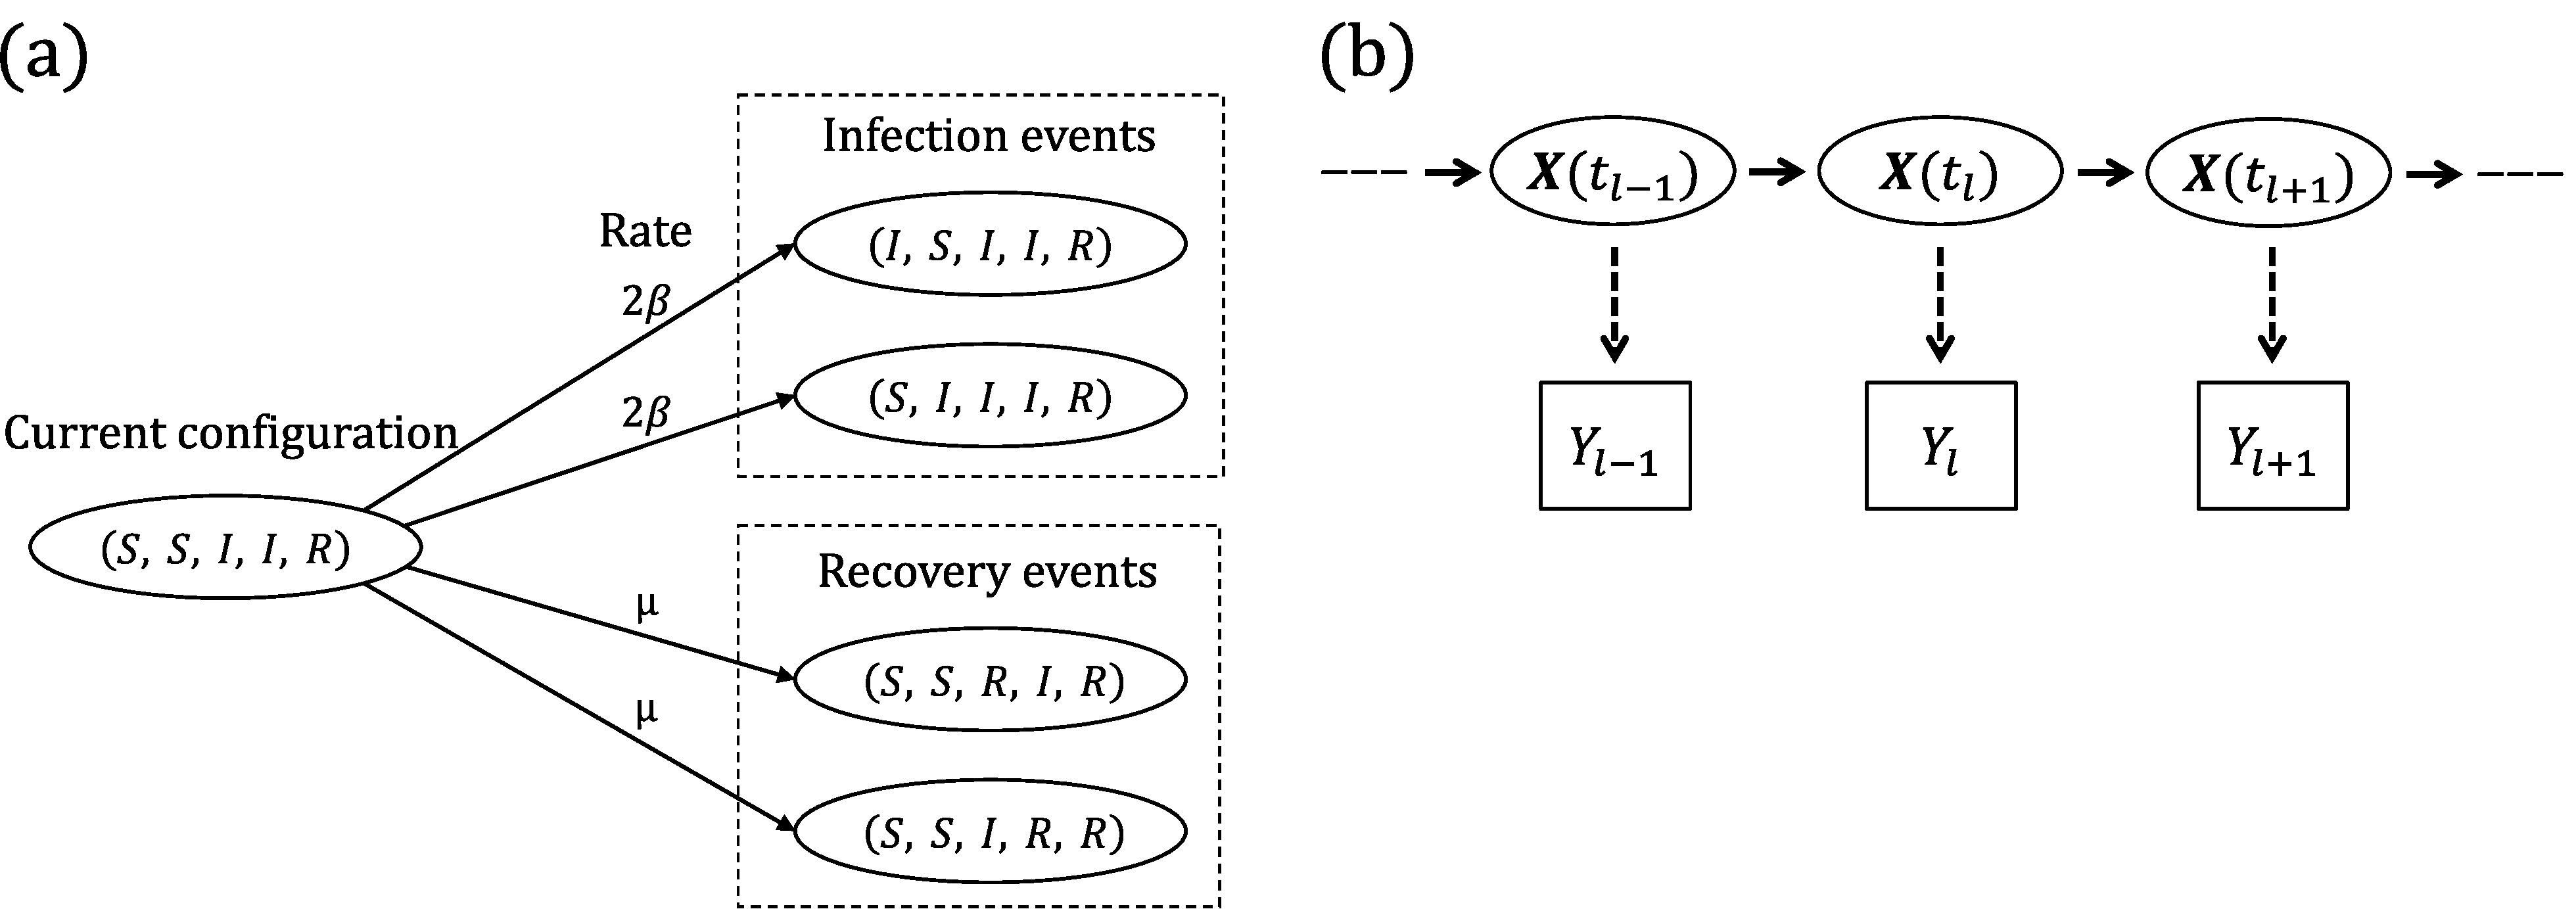
\includegraphics[width=0.95\linewidth]{figures/SIRdynamics_HMM}
	\caption[Diagram of subject--level state transitions and HMM structure for an SIR model.]{(a) SIR dynamics in a population of five subjects. The number of infecteds can increase from two to three via an infection of the first or second subject, reaching each of those configurations at rate $ 2\beta $. The number of recovered individuals can increase from one to two via a recovery of the third or fourth subject, reaching each of those configurations at rate $ \mu $. (b) Hidden Markov model for the joint distribution of the latent epidemic process and the data. The observations, $\mathbf{Y}_\ell,\ \ell=1,\dots,L$, are conditionally independent given $\bX(t)$, and $ \bY_\ell | I_{t_\ell}, \rho\sim\mathrm{Binomial}(I_{t_\ell}, \rho) $.}
	\label{fig:bda_SIRdynamics_HMM}
\end{figure}

\subsection{Subject--path proposal framework}
\label{subsec:bda_subj_proc}
The observed data likelihood in the posterior  $$ \pi(\btheta|\bY) \propto \pi(\bY|\btheta)\pi(\btheta)=\int L(\bY|\bX, \btheta) \pi(\bX|\btheta) \pi(\btheta) \rmd\bX$$
is analytically intractable for even moderately sized $ N $ as it involves a  high dimensional integral over the collection of subject--paths, $ \bX $. DA methods introduce the subject--paths, $ \bX $, as latent variables in the model that are jointly estimated along with the model parameters, $ \btheta $. Introducing $ \bX $ in this way enables us to work with the tractable complete data likelihood, (\ref{eqn:bda_comp_data_likelihood}). The joint posterior distribution is \begin{equation}
\label{eqn:bda_jointpost}
\pi(\btheta, \bX| \bY) \propto \Pr(\bY|\bX,\rho) \times\pi(\bX|\bX(t_1),\beta,\mu) \times \Pr\left (\bX(t_1)|\bp_{t_1}\right) \times\pi(\beta)\pi(\mu) \pi(\rho) \pi(\bp_{t_1}),
\end{equation} where $ \pi(\beta)$, $\pi(\mu)$, $\pi(\rho)$, and $\pi(\bp_{t_1}) $ are prior densities. Our MCMC targets the joint posterior distribution, given by (\ref{eqn:bda_jointpost}), as we alternate between updating $ \bX|\btheta,\bY $ and $ \btheta|\bX,\bY $. 

Given the current collection of subject--paths, $ \xcur $, we propose $ \xnew $ by sampling the path of a single subject $\bX_j$, conditionally on the data, using a time--inhomogeneous CTMC with state space $ \mcS_j  $ and rates conditioned on the collection of disease histories of other individuals, $ \bx_{(-j)}  = \lbrace \bx_1,\dots,\bx_{j-1},\bx_{j+1},\dots,\bx_N \rbrace$. The proposed collection of paths is accepted or rejected in a Metropolis--Hastings step. 

Let $ \btau^{(j)} = \lbrace \tau_\mathrm{I}^{(j)},\tau_\mathrm{R}^{(j)}\rbrace $ be the (possibly empty) set of infection and recovery times for subject $ j $, and define $ \btau^{(-j)} = \lbrace\btau\setminus\btau^{(j)}\rbrace = \left \lbrace \tau_0^{(-j)} ,\tau_1^{(-j)}, \dots, \tau_{M}^{(-j)}, \tau_{M+1}^{(-j)}\right \rbrace$, where $ t_1 \equiv \tau_0^{(-j)} $ and $ t_L\equiv\tau_{M+1}^{(-j)} $, to be the set of $ M\leq K $ (ordered) times at which other subjects become infected or recover, along with $ t_1$ and $ t_L $. Let $ \mcI = \lbrace \mcI_1, \dots,\mcI_{M+1}\rbrace $ be the intervals that partition $ [t_1,t_L]$, i.e. $ \mcI_1 = \left [\tau_0^{(-j)},\tau_1^{(-j)}\right ),\ \mcI_2=\left [\tau_1^{(-j)},\tau_2^{(-j)}\right ),\dots,\ \mcI_{M+1}=\left [\tau_{M}^{(-j)},\tau_{M+1}^{(-j)}\right )$. Let $ I_\tau^{(-j)} = \sum_{i\neq j}\ind{\bX_i(\tau) = I} $ be the prevalence at time $ \tau $, excluding subject $ j $. Let $ \bLambda^{(-j)}(\btheta) = \left \lbrace\bLambda_1^{(-j)}(\btheta),\dots,\bLambda_{M+1}^{(-j)}(\btheta) \right \rbrace$ be the sequence of rate matrices corresponding to each interval in $ \mcI $, where for $ m=1,\dots,M+1 $,
\begin{equation} \bLambda_m^{(-j)}(\btheta) = \bordermatrix{ & S & I & R \cr
	S & -\beta I_{\tau_m}^{(-j)} & \beta I_{\tau_m}^{(-j)} & 0 \cr 
	I & 0 & -\mu & \mu \cr
	R & 0 & 0 & 0 }.
\end{equation}
We can construct the transition probability matrix for subject $ j $ over interval $ I_m $, $$ \bP^{(j)}(\tau_{m-1},\tau_m) = \left (
p_{a,b}^{(j)}(\tau_{m-1},\tau_m)\right )_{a,b\in \mcS_j}, $$ where $ p_{a,b}^{(j)}(\tau_{m-1},\tau_m) = \Pr(\bX_j(\tau_m)=b|\bX_j(\tau_{m-1})=a, \btheta) $, using the matrix exponential $$
	\bP^{(j)} (\tau_{m-1},\tau_m)= \exp\left [(\tau_m - \tau_{m-1})\bLambda^{(-j)}_m(\btheta)\right ].
	$$
This computation requires an eigen--decomposition of each rate matrix. We may reduce the total computational burden by computing the eigen decompositions analytically, and by caching the decompositions to avoid duplicate computations. One additional point is that while the eigenvalues of any SIR rate matrix are always real valued, this is not generally true, e.g., it is possible for the rate matrix of an SIRS model to have complex eigenvalues. In this case, we obtain a real valued transition probability matrix by first applying a rotation to each rate matrix with complex eigenvalues to obtain its real canonical form \cite{hirsch2013differential}. This is discussed in Section \ref{sec:mtx_exp}.

By the Markov property, the time--inhomogeneous CTMC density over the observation period $ [t_1,t_L] $, denoted $ \pi(\bX_j | \bx_{(-j)}, \btheta) \equiv \pi\left (\bX_j | \bLambda^{(-j)}(\btheta); \mathcal{I}\right ) $, can be written as a product of time--homogeneous CTMC densities over the inter--event intervals $ \mcI_1,\dots,\mcI_{M} $. Hence,
\begin{equation}
\label{eqn:subj_level_dens}
\pi\left (\bX_j | \bLambda^{(-j)};\mathcal{I}\right ) = \Pr(\bX_j(t_1) | \bp_{t_1}) \prod_{m=1}^{M}\pi\left (\bX_j  | \bx_j(\tau_{m-1}), \bLambda^{(-j)}_m(\btheta);\mcI_m\right ).
\end{equation} 
Similarly, the transition probability matrix over an interval $ \mathcal{I}_\ell = [t_{\ell-1},t_\ell] $ can be written as the product of transition probability matrices over the sub--intervals in $ \mathcal{I}_\ell $, within which the subject--level CTMC is time--homogeneous. Thus, the transition probability matrix over an inter--observation interval, $ \mcI_\ell = [t_{\ell-1}, t_\ell] $, partitioned by $ S $ transition events that define inter--event intervals with endpoints given by times $ t_{\ell-1} \equiv \tau_{\ell,0}^{(-j)} < \tau_{\ell,1}^{(-j)}<\dots<\tau_{\ell,S-1}^{(-j)}  < \tau_{\ell,S}^{(-j)} \equiv t_\ell $, is constructed as
\begin{equation*}\label{eqn:inhomog_tpmprod} \bP^{(j)}(t_{\ell - 1},t_\ell) = \prod_{s=1}^{S}\bP^{(j)}\left(\tau_{\ell,s-1}^{(-j)},\tau_{\ell,s}^{(-j)}\right) .\end{equation*}

The algorithm for constructing a subject--path proposal proceeds in three steps, diagrammed in Figure \ref{fig:sampling_diagram}:  
\begin{enumerate}[nolistsep]
	\item \textit{HMM step}: sample the disease state of the subject under consideration at the observation times, conditional on the data and disease histories of other subjects.
	\item \textit{Discrete time skeleton step}: sample the state at times when the time--inhomogeneous CTMC rates change, conditional on the states sampled in the HMM step. 
	\item \textit{Event time step}: sample the exact times of transition events conditional on the sequence of states sampled in the previous steps. 
\end{enumerate}

\begin{figure}[htbp]
	\centering
	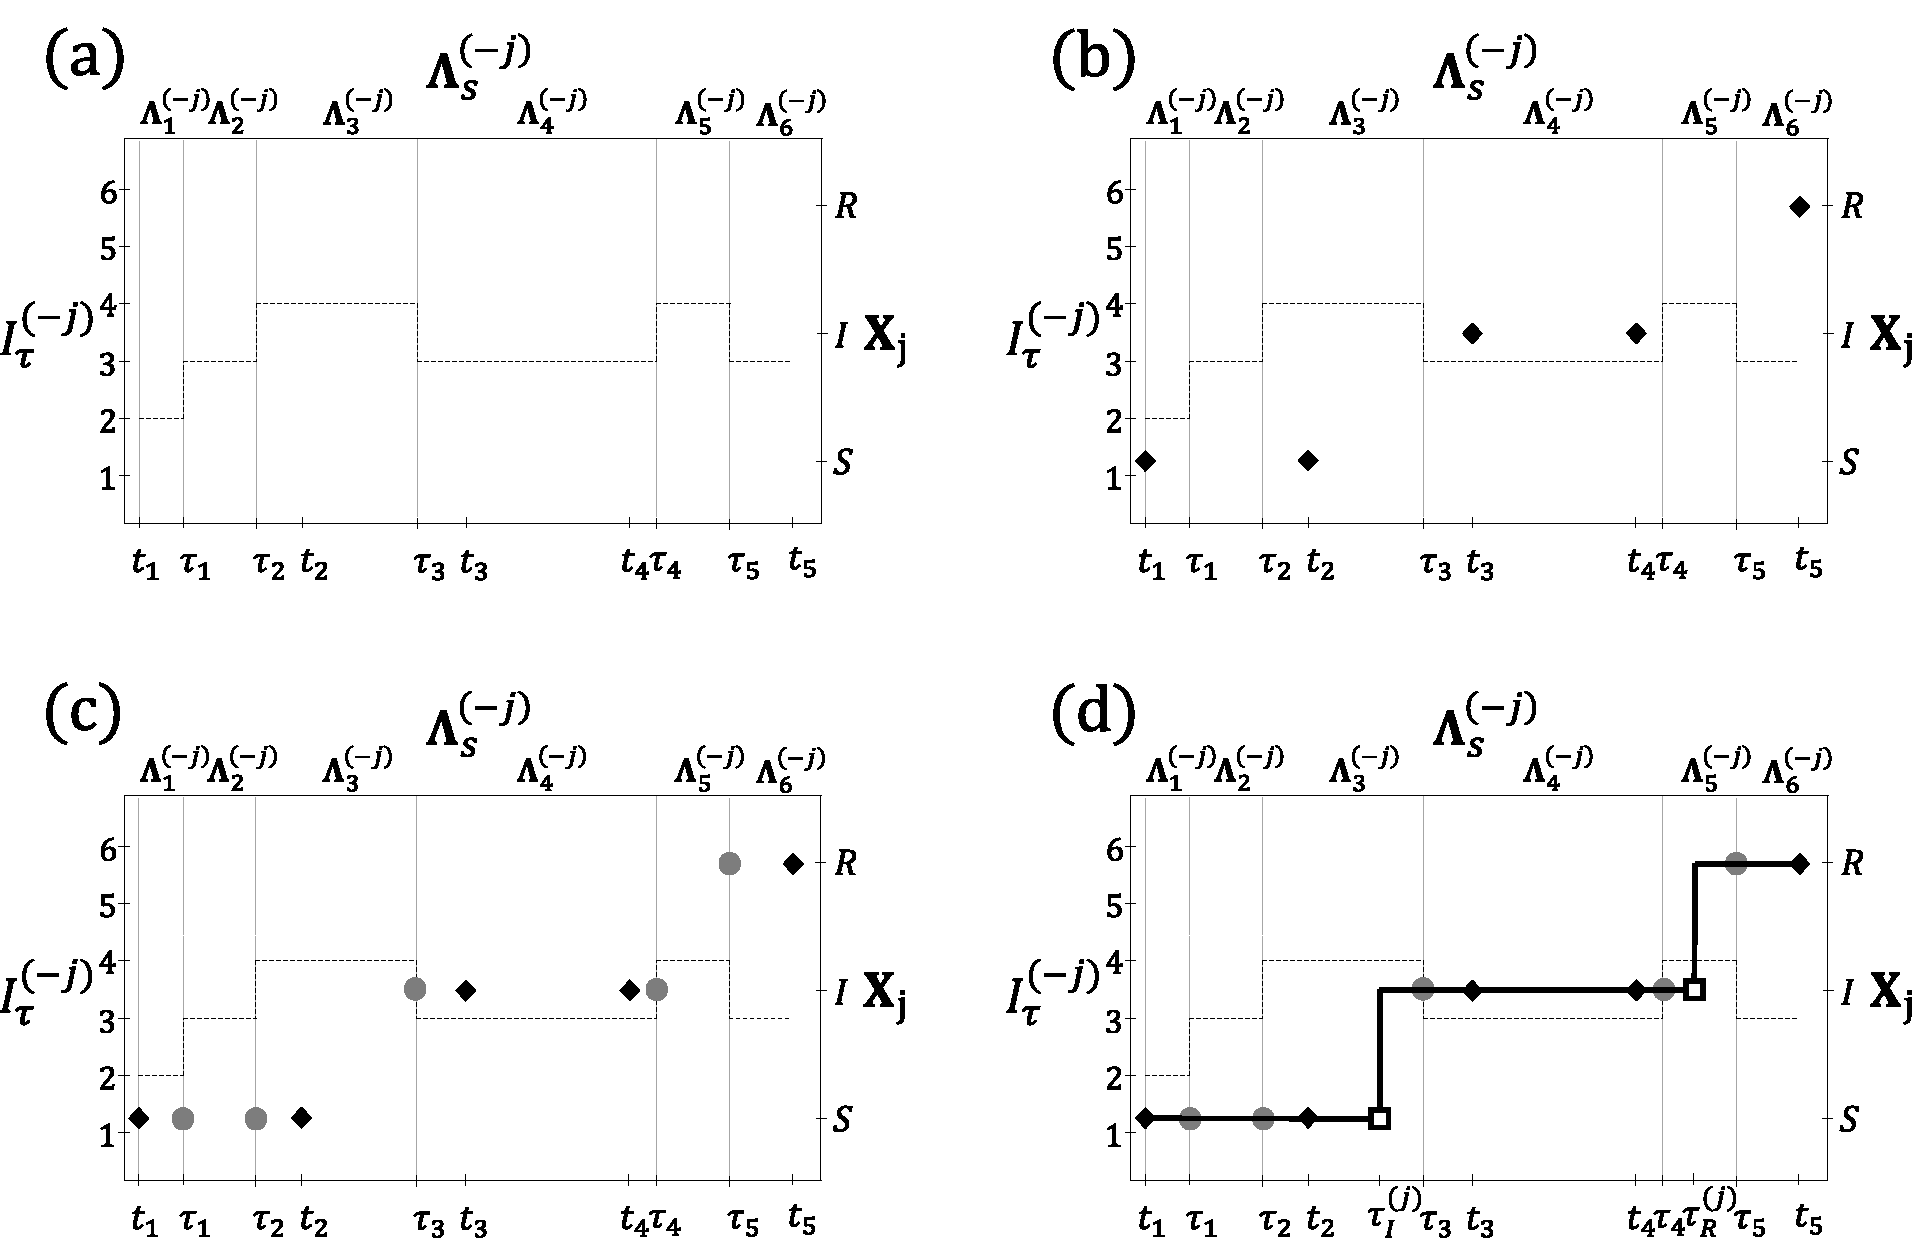
\includegraphics[width=0.95\linewidth]{figures/sampling_diagram.pdf}
	\caption[Diagram of subject--path proposals used in fitting models via Bayesian data augmentation.]{Procedure for constructing a subject--path proposal with SIR dynamics. (a) The dashed line depicts the number of infected individuals, excluding $ \bX_j $, the subject whose path is being sampled. The observation times, $ t_1,\dots,t_5 $, and times at which other subjects change disease states, $ \tau_1,\dots,\tau_5 $, are shown on the bottom axis. Rate matrices of the time--inhomogeneous CTMC (top axis) are constant within inter--event intervals (vertical lines). The state space of the subject--level process, $ \bX_j $, is shown on the right axis. (b) \textit{HMM step}: Sample the state of $ \bX_j $ at $ t_1,\dots,t_5 $, conditional on the data and on the disease histories of other subjects. (c) \textit{Discrete time skeleton step}: Sample the infection status at  $ \tau_1,\dots,\tau_5 $, conditional on the sequence of states sampled in the HMM step. (d) \textit{Event time step}: Sample the infection and recovery times from endpoint-conditioned time--homogeneous CTMC distributions, conditional on the sequence of disease states sampled in the HMM and discrete time skeleton steps.}
	\label{fig:sampling_diagram}
\end{figure}

\subsubsection{HMM step}
The key to sampling a sequence of disease states at the observation times is to rewrite the emission probability, given by (\ref{eqn:bda_emit_dist}), as
\begin{equation}\label{eqn:hmm_emit}
Y_\ell| X_j(t_\ell), I_{t_\ell}^{(-j)},\rho \sim \mathrm{Binomial}\left (\ind{X_j(t_\ell)=I} + I_{t_\ell}^{(-j)}, \rho\right ).
\end{equation}
If we treat the paths of all subjects except individual $ j $ as fixed, the emission probability in (\ref{eqn:hmm_emit}) only varies depending on whether subject $ j $ is infected at time $ t_\ell $. Furthermore, the data are conditionally independent of one another, given $ \bx$ and $ \btheta $, which induces a hidden Markov model (HMM) over the joint distribution $ \bX $ and $ \bY $ (Figure \ref{fig:bda_SIRdynamics_HMM}b). 

We sample the state of $ \bX_j $ at times $ t_1,\dots,t_L $ from the conditional distribution of $ \bX_j $, denoted $ \pi(\bX_j | \bY,\bx_{(-j)}, \btheta; t_1,\dots,t_L) $, using the stochastic forward--backward algorithm \cite{scott2002}. The algorithm enables us to efficiently sample from $ \pi\left (\bX \mid \bY, \bX_{(-j)}, \btheta\right ) $ by recursively accumulating, in a ``forward'' pass, information about the probability of various paths through $ \mcS $, conditional on the data, and then recursively sampling a trajectory in a ``backwards'' pass. 

In the forward recursion, we construct a sequence of matrices $ \bQ^{(t_2)}_j,\dots,\bQ^{(t_L)}_j $, where $ \bQ^{(t_\ell)}_j = \left (q_{j,r,s}^{(t_\ell)}\right )$, and $ q_{j,r,s}^{(t_\ell)} = \Pr\left (\bX_j(t_\ell) = s, \bX_j(t_{\ell - 1}) = r \mid \bY_{t_1}^{t_{\ell}},\bX_{(-j)},\btheta \right )$. Let $ \bP^{(j)}_{r,s}(t_{\ell - 1},t_\ell) = \Pr\left (\bX_j(t_\ell) = s \mid \bX(t_{\ell-1})=r, \btheta; \bX_{(-j)}\right ) $. If there are changes in the numbers of infected individuals in interval $ \mathcal{I}_\ell $, we construct the transition probability matrix for that interval as in (\ref{eqn:inhomog_tpmprod}). Then, 
\begin{equation}
q_{j,r,s}^{(t_\ell)} \propto \pi_{j}^{(t_\ell)}\left (r \mid \bX_{(-j)}, \btheta\right ) \times \bP^{(j)}_{r,s}\left (t_{\ell-1},t_\ell\right ) \times f\left (Y_{t_\ell} \mid \bX_j(t_\ell),\bX_{(-j)}(t_\ell), \rho, \bp_{t_1}\right ),	
\end{equation}
where $  \pi_{j}^{(t_\ell)}\left (r \mid \bX_{(-j)}, \btheta, \rho\right ) = \sum_r q_{j,r,s}^{(t_j)}$ and with proportionality reconciled via $ \sum_r\sum_s q_{j,r,s}^{(t_j)}=1 $.

In the backwards recursion, we sample the sequence of states at times $ t_1,\dots,t_L $ from the distribution $ \pi\left (\bX \mid \bY, \bX_{(-j)},\btheta, \rho,\bp_{t_1}\right )$. To do this, we first note that\vspace{-0.25in}

\begin{scriptsize}
	\begin{align*}\scriptsize
	\pi\left (\bX \mid \bY, \bX_{(-j)},\btheta, \rho,\bp_{t_1}\right ) &= \pi\left (\bX_j(t_L) \mid \bY_{t_1}^{t_L}, \bX_{(-j)},\btheta,\rho, \bp_{t_1}\right ) \prod_{\ell = 1}^{L-1}\pi \left (\bX_j(t_{L-\ell}) \mid \bX_{j,t_{L-\ell+1}}^{t_L}, \bX_{(-j)}, \bY_{t_1}^{t_L}, \btheta, \rho, \bp_{t_1}\right )\\
	&= \pi\left (\bX_j(t_L) \mid \bY_{t_1}^{t_L}, \bX_{(-j)},\btheta,\rho, \bp_{t_1}\right ) \prod_{\ell = 1}^{L-1}\pi \left (\bX_j(t_{L-\ell}) \mid \bX_{j,t_{L-\ell+1}}, \bX_{(-j)}, \bY_{t_1}^{t_{L-\ell+1}}, \btheta, \rho, \bp_{t_1}\right ),
	\end{align*}
\end{scriptsize} 
\hspace{-0.05in}where the second equality follows from the conditional independence of the HMM. We proceed by first drawing $ \bX_j(t_L) $ from $ \pi_j^{(t_L)}\left (\cdot \mid \bX_{(-j)}, \btheta,\rho\right  ) $, and then drawing $ \bX_j(t_\ell),\ \ell = L-1,\dots,1, $ each in turn from the categorical distribution with masses proportional to column $ \bx_j(t_{\ell+1}) $ of $ \bQ_j^{(t_{\ell+1})} $. 

\subsubsection{Discrete-time skeleton step}
It would be straightforward to sample the exact infection and recovery times of subject $ j $, conditional on the sequence of states at times $ t_1,\dots, t_L $, if the subject--level CTMC rates did not possibly vary over each inter--observation interval. We may reduce our problem to the time--homogeneous case by first sampling the disease state at the intermediate event times when the CTMC rates change, and then sampling the full path within each inter--event interval. Consider an inter--observation interval, $ \mcI_\ell = [t_{\ell-1}, t_\ell] $, containing inter--event intervals whose endpoints are given by times $ t_{\ell-1} \equiv \tau_{\ell,0}^{(-j)} < \tau_{\ell,1}^{(-j)}<\dots<\tau_{\ell,n-1}^{(-j)}  < \tau_{\ell,n}^{(-j)} \equiv t_\ell $. We recursively sample $ \bX_j $ at each intermediate event time, beginning at $ \ttau_1 $, from the discrete distribution with masses 
\begin{align}
&\Pr\left (\bX_j\left (\ttau_{i}\right ) = x_{i} \mid  \bX_j\left (\ttau_{i-1}\right ) = x_{i-1}, \bX_j\left (\ttau_{n}\right ) = x_n\right ) \nonumber \\  &\hspace{1in}= \frac{\Pr\left (\bX_j\left (\ttau_{i}\right ) = x_{i}, \bX_j\left (\ttau_{i-1}\right ) = x_{i-1}, \bX_j\left (\ttau_{n}\right ) = x_n\right )}{\Pr\left (\bX_j\left (\ttau_{i-1}\right ) = x_{i-1}, \bX_j\left (\ttau_{n}\right ) = x_n\right )} \nonumber\\
&\hspace{1in}= \frac{\Pr\left (\bX_j\left (\ttau_{i}\right ) = x_{i} \mid \bX_j\left (\ttau_{i-1}\right ) = x_{i-1}\right )\Pr\left (\bX_j\left (\ttau_{n}\right ) = x_n \mid \bX_j\left (\ttau_{i}\right ) = x_{i}\right )}{\Pr\left (\bX_j\left (\ttau_{n}\right ) = x_n | \bX_j\left (\ttau_{i-1}\right ) = x_{i-1}\right)} \nonumber\\
&\hspace{1in} = \frac{\left [\bP^{(j)}\left (\ttau_{i-1},\ttau_{i}\right )\right ]_{x_{i-1},x_{i}}\left [\prod_{k=i}^{n-1}\bP^{(j)}\left (\ttau_{k}, \ttau_{k+1}\right )\right ]_{x_{i},x_n}}{\left [\prod_{k=i-1}^{n-1}\bP^{(j)}\left (\ttau_{k}, \ttau_{k+1}\right )\right]_{x_{i-1},x_n}}.
\label{eqn:dt_skel}
\end{align}

\subsubsection{Event time step}
The final step in constructing a subject--path is to sample the exact infection and recovery times given the discrete sequence of states obtained in the previous two steps. This amounts to simulating the path of an endpoint--conditioned time--homogeneous CTMC, a task for which there exist a variety of efficient methods \cite{hobolth2009}. When fitting the SIR model, we chose to use modified rejection sampling, a modification of Gillespie's direct algorithm \cite{gillespie1976general} that explicitly avoids simulating constant paths. This method is known to be efficient when the states differ at the endpoints of small time intervals. We used uniformization--based sampling \cite{hobolth2009} when fitting SEIR and SIRS models, which was more robust when sampling paths in intervals with multiple transitions. Fast implementations of these methods are available in the \texttt{ECctmc} package in \texttt{R} \cite{ECctmc}. We briefly summarize the algorithms below, and refer to \cite{hobolth2009} for a more thorough discussion.   

Our goal is to simulate a path for a time--homogeneous CTMC, $ \bX $, in the interval $ [0,T] $, conditional on $ \bX(0) = a $ and $ \bX(T) = b $. Let $ \bLambda $ be the rate matrix for the process. Let $ \Lambda_{a} $ denote the $ a,a $ diagonal element of $ \bLambda $, and similarly let $ \Lambda_{a,b} $ denote the rate given by the $ a,b $ element. We also denote by $ \mathbf{P}(T) $ the transition probability matrix for the CTMC over $ [0,T] $, and $ P_{ab}(T) $ the probability of beginning in state $ a $ and ending in state $ b $.

The modified rejection algorithm proposes paths by explicitly sampling the first transition time when it is known that at least one transition occurred (i.e. when $ a  \neq b $). The remainder of the path is proposed by forward sampling, using, for instance, Gillespie's direct algorithm. The proposed path is accepted if $ \bX(T) = b $. If a transition is not known to have occurred (i.e. when $ a = b $), a path is proposed via ordinary forward simulation and accepted if $ \bX(T) = b $. We sample the first transition time via the inverse--CDF method, sampling $ u\sim \mathrm{Unif}(0,1) $ and applying the inverse-CDF function 
\begin{equation} F^{-1}(u) = \frac{-\log\left [1 - u \times \left (1 - \e^{-T\Lambda_a}\right )\right ]}{\Lambda_a}. 
\end{equation}

We found that the modified rejection algorithm worked well in fitting the SIR and SIRS models. In the examples we studied in which these models were fit, subject--paths over intervals where the endpoints required multiple jumps ($ S \rightarrow R $, or $ I \rightarrow S $) were almost never considered. Usually, only a single transition time was sampled in a given interval, so the inverse--CDF method was fast.

The uniformization algorithm samples the path for a time--homogeneous CTMC conditional on the state at the interval endpoints by coupling the original CTMC to the Markov chain for an auxilliary Poisson point process. State transitions, including virtual transition where the state does not change, are events of the point process, and the sequence of state labels is drawn from the corresponding Markov chain.

We construct the transition rate matrix of the auxilliary Markov chain, $ \bZ $, as $ R = I + \frac{1}{\mu}\bLambda $, where $ \mu = \max_a \bLambda_a$. The probability mass function for the number of state transitions, $ N $, conditional on $ \bX(0) = a,\ \bX(T) = b $, is
\begin{equation}
P(N=n|\bX(0) = a, \bX(T) = b) = \e^{-\mu T}\frac{(\mu T)^n}{n!}R_{ab}^n / P_{ab}(T).
\end{equation}
The algorithm proceeds by first sampling the number of state transitions from this distribution. If there are no transitions, or if there is one transition and the states at the endpoints are the same, the algorithm terminates. Otherwise, we drawn $ n $ independent uniform values in $ [0,T] $ and sort them to obtain the times of state transitions. The state labels at the sorted sequence of times, $ \tau_i $, $ i = 1,\dots,n-1 $, are drawn from the discrete distribution with masses given by
\begin{equation}
P(\bX(\tau_i) | \bX(\tau_{i-1}, \bX(T) = b) = \frac{R_{x_{i-1},x_i}(R^{n-i})_{x_ib}}{(R^{n-i+1})_{x_{i-1}b})}.
\end{equation}

Uniformization--based sampling was preferred in the case of the SEIR model since modified rejection sampling tended to get hung up when sampling paths in intervals where the endpoints suggested that at least two state transitions occured (which though it seldom occured, significantly slowed down the MCMC). We also note that the transition probability, $ P_{ab}(T) $, is computed and cached in executing the HMM step of our algorithm. Therefore, there are no additional eigen--decompositions or matrix exponentiations are required for the uniformization algorithm.

\subsubsection{Metropolis--Hastings step}
Having constructed a complete subject--path proposal, we decide whether to accept or reject it via a Metropolis--Hastings step. We emphasize that the true distribution of $ \bX_j | \bx_{(-j)},\btheta $ does not match the time--inhomogeneous CTMC in our proposal. Suppressing the dependence on $ \btheta $, the target distribution of the subject--path proposal is $ \pi(\bX | \bY) \propto\pi(\bY | \bX)\pi(\bX) $. Note that $ \xnew $ and $ \xcur $ differ only in the path of the $ j^{th} $ subject, so $ \Lambda^{(-j)}(\xcur) = \Lambda^{(-j)}(\xnew)=\bLambda^{(-j)} $.

Suppressing the dependence on $ \btheta$ for clarity, the acceptance ratio is
\begin{equation*}
a_{\xcur \longrightarrow \xnew} = \min \left \lbrace \frac{\pi(\xnew|\by)}{\pi(\xcur|\by)}\frac{q(\xcur|\xnew)}{q(\xnew|\xcur)},\ 1\right \rbrace
\end{equation*}
Now, 
\begin{eqnarray*}
	\pi(\xnew|\by) &\propto& \Pr(\by|\xnew)\pi(\xnew),\\
	\pi(\xcur|\by) &\propto& \Pr(\by|\xcur)\pi(\xcur),
\end{eqnarray*}
where $ \Pr(\by|\xnew) $ and $ \Pr(\by|\xcur )$ are binomial probabilities for the measurement process, and $ \pi(\xnew) $ and $ \pi(\xcur) $ are the time--homogenous CTMC densities of the current and the proposed population--level paths that appear in Equation (\ref{eqn:bda_comp_data_likelihood}). Let $ \pi(\xnew_j|\bLambda^{(-j)}; \mcI) $ and $ \pi(\xcur_j| \bLambda^{(-j)}; \mcI) $ denote the time--inhomogeneous subject--level CTMC proposal densities given by (\ref{eqn:subj_level_dens}). Then,
\begin{align*}
	q(\xnew|\xcur) &= \Pr(\xnew|\by; \bLambda^{(-j)}(\xcur), \mcI)\\
	&= \frac{\pi(\xnew, \by; \bLambda^{(-j)}(\xcur), \mcI)}{\Pr(\by; \bLambda^{(-j)}, \mcI)}\\
	&= \frac{\Pr(\by|\xnew)\pi(\xnew_j| \bLambda^{(-j)}; \mcI)}{\Pr(\by; \bLambda^{(-j)}(\xnew), \mcI)}\\
	\shortintertext{and similarly, } q(\xcur|\xnew) &= \frac{\Pr(\by|\xcur)\pi(\xcur_j| \bLambda^{(-j)}; \mcI)}{\Pr(\by; \bLambda^{(-j)}(\xcur), \mcI)}.
\end{align*}
Therefore, 
\begin{align*}
	\frac{\pi(\xnew|\by)}{\pi(\xcur|\by)}\frac{q(\xcur|\xnew)}{q(\xnew|\xcur)} &= \frac{\Pr(\by|\xnew)\pi(\xnew)}{\Pr(\by|\xcur)\pi(\xcur)}\frac{\Pr(\by|\xcur)\pi(\xcur_j; \bLambda^{(-j)})}{\Pr(\by|\xnew)\pi(\xnew_j; \bLambda^{(-j)})}\\
	&= \frac{\pi(\xnew)}{\pi(\xcur)}\frac{\pi(\xcur_j| \bLambda^{(-j)}; \mcI)}{\pi(\xnew_j| \bLambda^{(-j)}; \mcI)}.
\end{align*}
Hence, the Metropolis--Hastings acceptance probability is
\begin{equation*}
a_{\xcur \longrightarrow\xnew}=\min \left \lbrace  \frac{\pi(\xnew)}{\pi(\xcur)}\frac{\pi(\xcur_j| \bLambda^{(-j)}; \mcI)}{\pi(\xnew_j| \bLambda^{(-j)}; \mcI)} , 1 \right \rbrace, 
\end{equation*}
which depends on the ratio is of the population-level time--homogeneous CTMC densities, multiplied by the ratio of time--inhomogeneous CTMC proposal densities. 

\subsubsection{Initializing the collection of subject--paths}
We initialize the collection of subject paths at the start of our MCMC by simulating paths using Gillespie's direct algorithm \cite{gillespie1976general} until we have found a path under which the data have non--zero probability. 
A sufficient condition for this under the binomial sampling model is that the number of infected individuals is greater than the observed prevalence at each observation time. 

\subsection{Parameter Updates and MCMC Scan Order}
\label{subsec:bda_mcmc_scan}
One MCMC iteration includes a number of subject--path updates, followed by a set of parameter updates. Conjugate priors were available for all parameters of the models in this chapter. Therefore, we chose to use Gibbs sampling to update parameter values from their univariate full conditional distributions (below).

There is no need to re--sample the path of every subject within each MCMC iteration. Indeed, we might suspect that the efficiency of our MCMC could be improved by sampling only a few subject--paths between parameter updates. Successive subject--path proposal tend to be highly autocorrelated, as with other DA methods \cite{roberts2001}, and incur a relatively high computational cost. Frequently updating model parameters may help to break this correlation, despite the strong autocorrelations in posterior samples of model parameters. Often, the effective sample size (ESS) per CPU time is optimized by sampling only a handful of subject--paths per MCMC iteration. However, many factors, including the SEM dynamics, population size, efficiency of the implementation, and the degree of model misspecification could affect the optimal number subject--path updates per MCMC iteration. It is clearly impossible to disentangle all possible factors affecting the optimal number of subject--path updates per iteration. Therefore, we set the number of subject--paths per iteration on the basis of log--posterior ESS per CPU time in an initial run of 5,000--10,000 iterations.

\subsection{Data augmentation for SEIR dynamics}
\label{subsec:bda_seir_model}

The SEIR model adds a latent state to the SIR model in which subjects who are exposed to an infected individual incubate before becoming infectious. As with the SIR model, recovery is assumed to confer lifelong immunity. The structure of this model does not affect any of the machinery involved in the subject--path proposal mechanism, but rather merely redefines the population--level time--homogeneous CMTC for the epidemic process, and the subject--level time--inhomogeneous CTMC used in the subject--path proposals.

Under this model, we suppose that the data are sampled from a latent epidemic process, $ \bX = \lbrace \bX_1,\dots,\bX_N\rbrace $, that evolves in continuous--time as individuals become exposed, infectious, and recover. The state space of this process is $ \mcS = \lbrace S,E,I,R\rbrace^N $, the Cartesian product of $ N $ state labels taking values in $ \lbrace S,E,I,R\rbrace $. The state space of a single subject, $ \bX_j $, is $\mcS_j = \lbrace S, E, I, R\rbrace $, and a realized subject--path is of the form $$ \bx_j(\tau) = \left (S,\ \tau < \tau^{(j)}_{\mathrm{E}};E,\  \tau^{(j)}_{\mathrm{E}} \leq \tau < \tau^{(j)}_{\mathrm{I}};I,\ \tau^{(j)}_{\mathrm{I}} \leq \tau < \tau^{(j)}_{\mathrm{R}};R\ ,\ \tau^{(j)}_{\mathrm{R}} \leq \tau
\right ) $$
where $ \tau^{(j)}_{\mathrm{E}} $, $ \tau^{(j)}_{\mathrm{I}} $, and $ \tau^{(j)}_{\mathrm{R}} $ are the times at which subject $ J $ becomes exposed, infectious, and recovers. As with the SIR model, some or all of these events may not transpire in the observation period $ [t_1,t_L] $, or at all. We let $ \beta $ be the per--contact infectivity rate, $ \gamma $ be the rate at which an exposed individual becomes infectious, and $ \mu $ be the rate at which an infectious individual recovers. Furthermore, we write the vector of disease state probabilities as $ \bp_{t_1} = (p_S,p_E,p_I,p_R) $. The latent epidemic process evolves according to a time--homogeneous CTMC, with transition rate from configuration $ \bx $ to $ \bx^\prime $ that differ only in the state of one subject $ j $ is given by $ \bLambda = \beta I $ if $ \bX_j = S $ and $ \bX^\prime_j = E$, $ \gamma $ if $ \bX_j = E $ and $ \bX^\prime_j = I$, and $ \mu $ if $ \bX_j = I $ and $ \bX^\prime_j = R$. Finally, the time--inhomogeneous CTMC rate matrices used in the subject--path proposal distribution have the form
\begin{equation} \bLambda_m^{(-j)}(\btheta) = \bordermatrix{ & S & E & I & R \cr
	S & -\beta I_{\tau_m}^{(-j)} & \beta I_{\tau_m}^{(-j)} & 0 & 0 \cr 
	E & 0 & -\gamma & \gamma & 0 \cr
	I & 0 & 0 & -\mu & \mu \cr
	R & 0 & 0 & 0 & 0 }.
\end{equation}
As with the SIR model, the eigenvalues of the CTMC rate matrices for the SEIR model are always real valued. The only computational modification, relative to the SIR model, that we suggest is that times of state transition in inter--event intervals be sampled conditional on the state at the endpoints via uniformization.

\subsection{Data augmentation for SIRS dynamics}
\label{subsec:bda_sirs_model}

The SIRS model modifies the SIR model to allow for loss of immunity. Again, fitting this model using our Bayesian data augmentation algorithm does not affect any of the machinery involved in the subject--path proposal mechanism, although the recurrent nature of the disease dynamics increases the computational burden since the disease state at the interval endpoints does not absolve us of sampling the full path within each inter--event interval where the states at the endpoints are the same.

Under the SIRS model, we suppose that the data are sampled from a latent epidemic process, $ \bX = \lbrace \bX_1,\dots,\bX_N\rbrace $, that evolves in continuous--time as individuals become exposed, infectious, and recover. The state space of this process is $ \mcS = \lbrace S,I,R\rbrace^N $, the Cartesian product of $ N $ state labels taking values in $ \lbrace S,I,R\rbrace $. The state space of a single subject, $ \bX_j $, is $\mcS_j = \lbrace S, I, R\rbrace $, and a realized subject--path is of the form $$ \bx_j(\tau) = \left (S,\ \tau < \tau^{(j)}_{\mathrm{I}_1}; 
	I,\ \tau^{(j)}_{\mathrm{I}_1} \leq \tau < \tau^{(j)}_{\mathrm{R}_1};
	R\ ,\ \tau^{(j)}_{\mathrm{R}_1} \leq \tau < \tau^{(j)}_{\mathrm{L}_1}; 
	S\ ,\ \tau^{(j)}_{\mathrm{L}_1} \leq \tau < \tau^{(j)}_{\mathrm{I}_2};\dots
	\right ), $$
where $ \tau^{(j)}_{\mathrm{I}_k} $, $ \tau^{(j)}_{\mathrm{R}_k} $, and $ \tau^{(j)}_{\mathrm{L}_k} $ are times at which subject $ J $ becomes infected, recovers, and loses immunity, and are ennumerated by the subscript $ k $ as the process may revisit each state multiple time. As with the SIR and SEIR models, it is possible that some or all of these events may not come about within the observation period $ [t_1,t_L] $. We let $ \beta $ be the per--contact infectivity rate, $ \mu $ be the rate at which an infectious individual recovers, and $ \gamma $ be the rate at which immunity is lost. We write the vector of disease state probabilities as $ \bp_{t_1} = (p_S,p_I,p_R) $. The latent epidemic process evolves according to a time--homogeneous CTMC, with transition rate from configuration $ \bx $ to $ \bx^\prime $ that differ only in the state of one subject $ j $ is given by $ \bLambda = \beta I $ if $ \bX_j = S $ and $ \bX^\prime_j = E$, $ \mu $ if $ \bX_j = I $ and $ \bX^\prime_j = R$, and $ \gamma $ if $ \bX_j = R $ and $ \bX^\prime_j = S$. Finally, the time--inhomogeneous CTMC rate matrices used in the subject--path proposal distribution have the form
\begin{equation} \bLambda_m^{(-j)}(\btheta) = \bordermatrix{ & S & I & R \cr
	S & -\beta I_{\tau_m}^{(-j)} & \beta I_{\tau_m}^{(-j)} & 0  \cr 
	I & 0 & -\mu & \mu \cr
	R & \gamma & 0 & -\gamma }.
\end{equation}
Unlike the SIR and SEIR models, eigenvalues of each CTMC rate matrix may be complex. In order to obtain a real valued transition probability matrix over an interval for which eigenvalues of the rate matrix are complex, we must rotate that rate matrix to obtain its real canonical form. This is further discussed in Section \ref{sec:mtx_exp}.

\section{Simulation results}
\label{sec:bda_simulations}

\subsection{Inference Under a Variety of Epidemic Dynamics}
\label{subsec:bda_sir_seir_sirs_sim}
We fit SIR, SEIR, and SIRS dynamics to binomially distributed prevalence counts sampled from epidemics simulated under corresponding dynamics in populations of 750, 500, and 200 individuals (details provided in Section \ref{sec:bda_sim1_details}). Priors for the rate parameters and binomial sampling probability were chosen so that the priors spanned reasonable ranges of values (e.g. recovery durations ranging from days to weeks/months rather than seconds to eons under extremely diffuse priors), but were otherwise only mildly informative, while the initial distribution parameters were assigned informative priors (see tables \ref{tab:sim1_sir_priors}, \ref{tab:sim1_seir_priors}, and \ref{tab:sim1_sirs_priors}). The three datasets, depicted in Figure \ref{fig:sim1_latent_posts} along with the estimated pointwise posterior prevalence, presented a range of challenges. The SIR example was arguably the most ``standard'' example as the observation period captured the exponential growth and decline of the epidemic. Thus, much of the curvature in the latent path was reflected in the data. In contrast, data from the outbreak simulated under near--endemic SEIR dynamics contained very little information about the shape of the epidemic curve. The task of disentangling whether the data were sampled with low probability from a high--prevalence outbreak, or visa--versa, was further complicated by the inclusion of an additional disease state --- the exposed state --- that was not directly observed. Finally, the SIRS model was more computationally challenging for two reasons. First, the recurrent nature of the disease process demanded that the disease state at each event time, and the path within each inter--event interval, be sampled in the subject--path proposal. Second, it was possible for CTMC rate matrices to have complex eigen--decompositions, which made computing transition probability matrices more expensive. This affected the optimal number of subject--path updates per MCMC iteration.

\begin{figure}[!h]
	\centering
	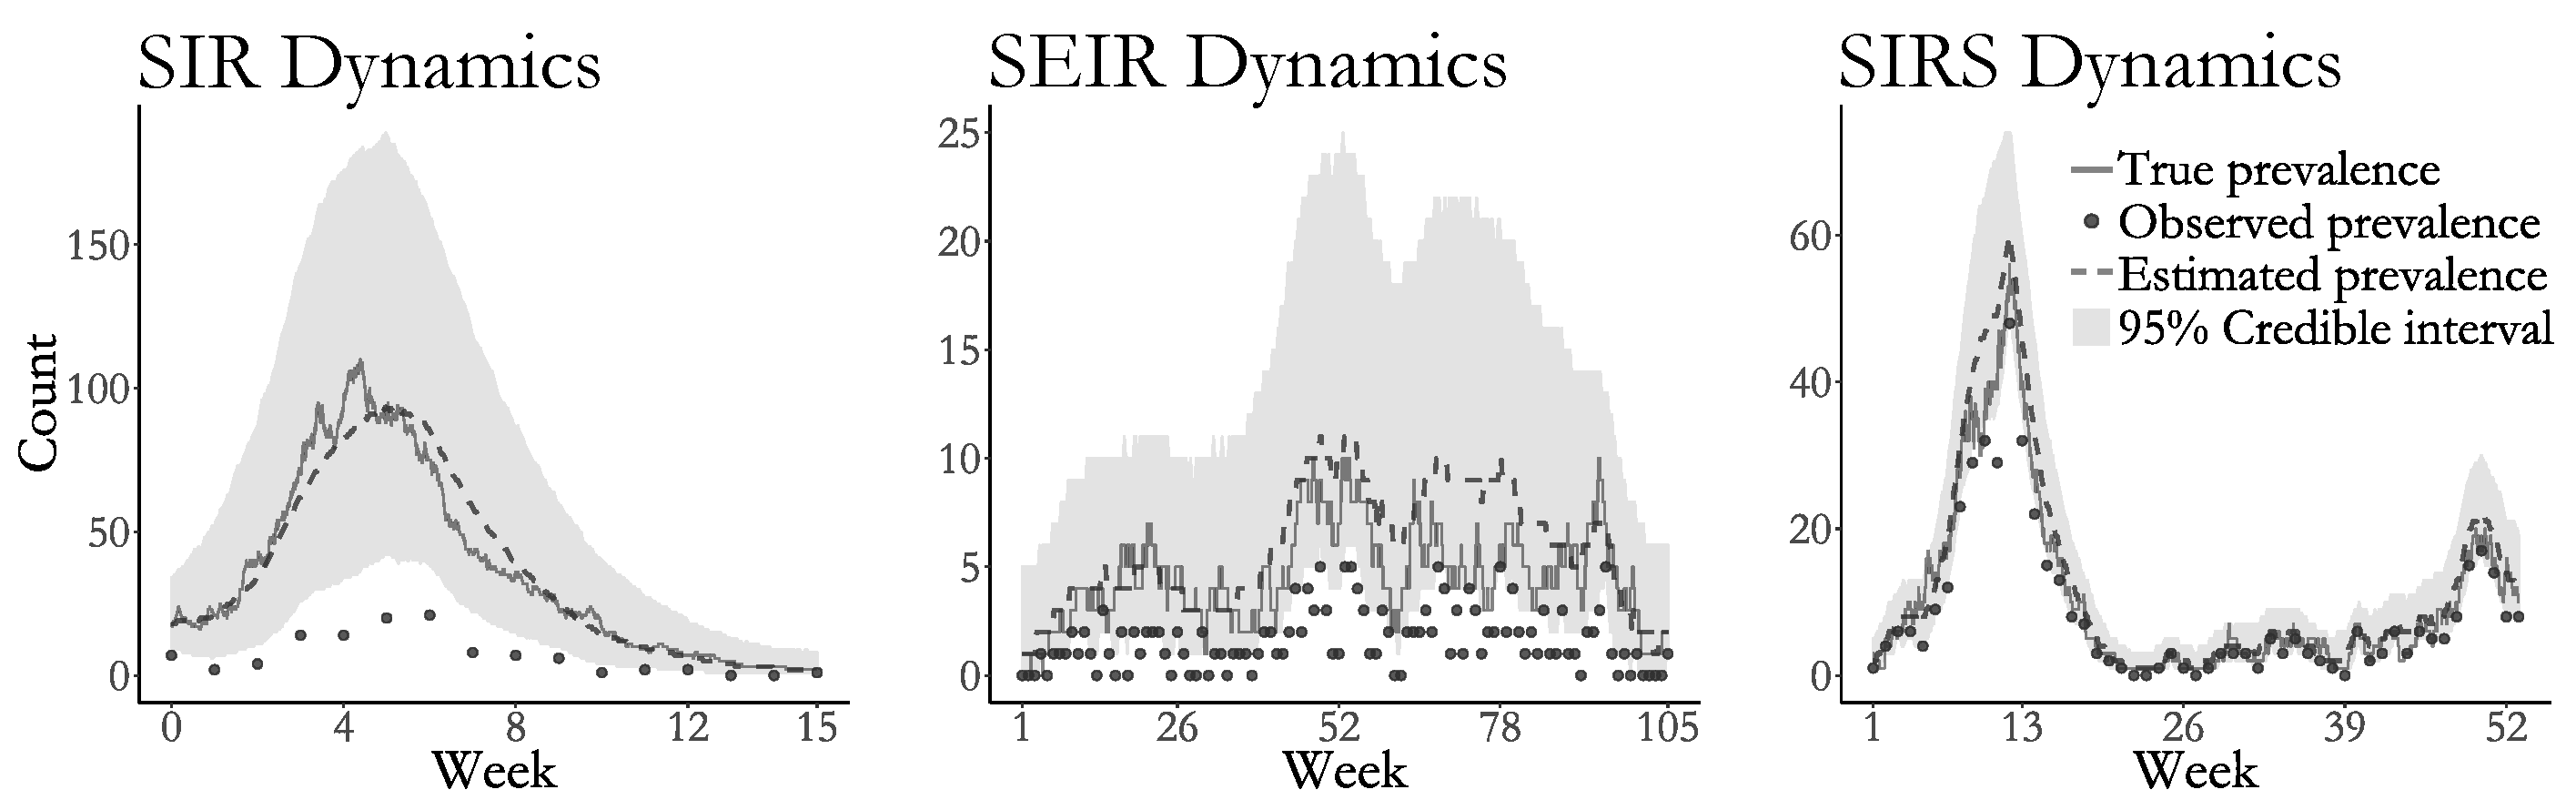
\includegraphics[width=\linewidth]{figures/sim1_latent_posts.pdf}
	\caption[Estimated latent posteriors for SIR, SEIR, and SIRS models fit to simulated prevalence data.]{Estimated latent posterior distributions of disease prevalence in outbreaks simulated under SIR (left), SEIR (middle), and SIRS (right) dynamics. Depicted are the true unobserved prevalence (solid line), observed data (dots), pointwise posterior median prevalence (dashed line), and pointwise 95\% credible intervals (shaded region). Latent posterior estimates are based on a thinned sample, with every $250^{th}$ sample retained.}
	\label{fig:sim1_latent_posts}
\end{figure}

The true epidemic paths and parameter values fell well within the 95\% Bayesian credible intervals in all three simulations (Figure \ref{fig:sim1_latent_posts} presents the estimated latent posterior prevalence; Figure \ref{fig:sim1_credint} presents posterior estimates of model parameters; Figure \ref{fig:sim1_latent_post_all} presents estimated latent posterior distributions and true epidemic paths for all model compartments). The acceptance rates for subject--path proposals were roughly 92\% for the SIR model, 91\% for the SEIR model, and 77\% for the SIRS model. Our posterior estimates of the model parameters also closely match estimates obtained using the particle marginal Metropolis--Hastings (PMMH) algorithm of \cite{andrieu2010particle}, implemented using the \texttt{pomp} package in \texttt{R} \cite{pomp}. We simulated particle paths in the PMMH algorithm in two ways; exactly using Gillespie's direct algorithm \cite{gillespie1976general}, and approximately using a multinomial modification of $ \tau $--leaping \cite{breto2011compound}. In these small population examples, the exact algorithm is arguably more appropriate, as the leap conditions for $ \tau $--leaping may not be met in small populations, but it is also substantially slower. In these simple settings, PMMH tended to outperform our algorithm in terms of log--posterior effective sample size (ESS) per CPU time. When PMMH particle paths were simulated by $ \tau $--leaping, the average ESS per CPU compared to BDA was roughly $ 350\times $ greater for the SIR model, $ 4.4\times $ greater for the SEIR model, and $ 13\times $ greater for the SIRS model. Exact simulation of PMMH particle paths reduced the computational advantage of PMMH substantially. In this case, the average log--posterior ESS per CPU time was $ 10.5\times $ greater for PMMH in fitting the SIR model, $ 2\times $ for the SEIR model, and $ 0.7\times $ for the SIRS model. These comparisons did not include the time required to tune the MCMC for PMMH, which was nontrivial. In contrast, our algorithm required no tuning beyond selecting the number of subject--paths to update per MCMC iteration. We also note that in fitting the models using PMMH, we were required to make several implementation decisions to prevent particle degeneracy and to balance speed with precision. These included selecting the number of particles and the time--step in the approximate $ \tau $--leaping algorithm. For example, when using $ \tau $--leaping to simulate particle paths, the number of particles required to obtain good mixing for the SIRS model fit with PMMH was higher than for the other two models. Details of the PMMH implementations and further results are presented in Section \ref{sec:bda_sim1_details}.

\begin{figure}[!h]
	\centering
	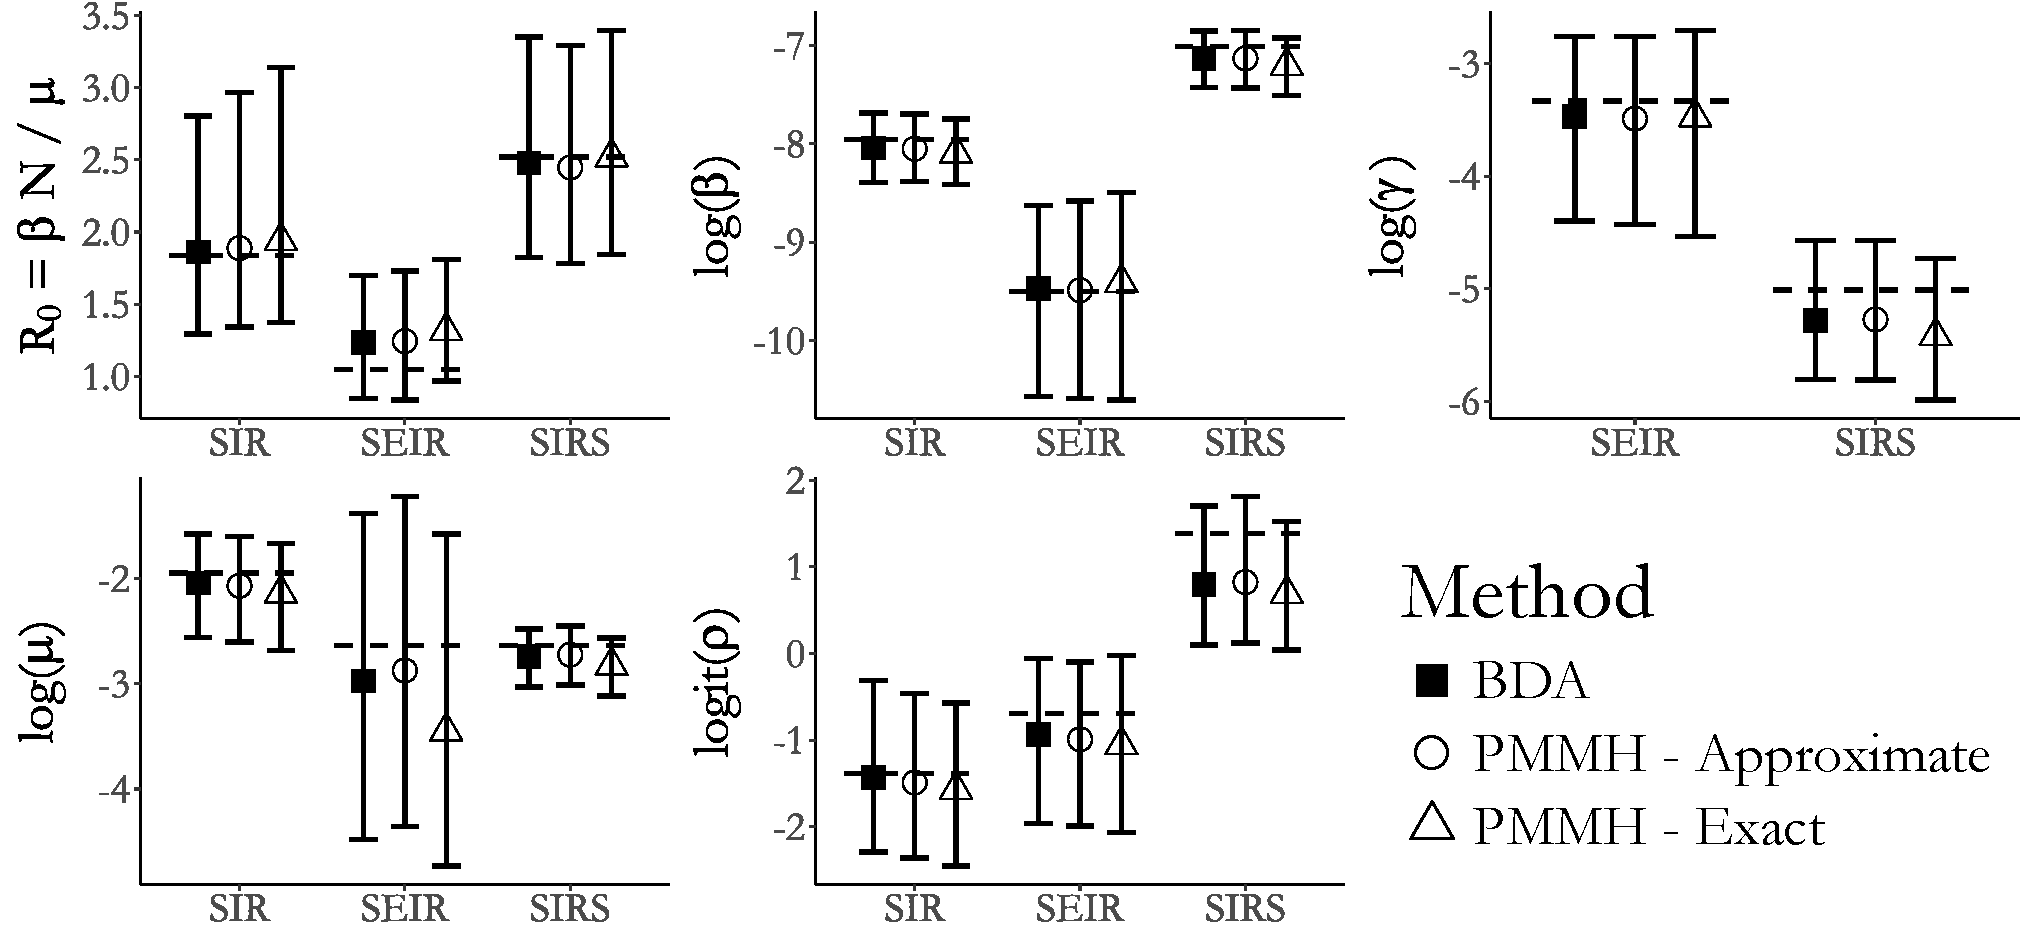
\includegraphics[width=\linewidth]{figures/sim1_credints.pdf}
	\caption[Posterior estimates of SIR, SEIR, and SIRS model parameters fit to simualted data using Bayesian data augmentation and PMMH.]{Posterior medians and 95\% credible intervals of parameters in the SIR, SEIR, and SIRS models fit with Bayesian data augmentation (BDA) and particle marginal Metropolis--Hastings (PMMH) with particle paths simulated approximately (using $ \tau $--leaping) and exactly (using Gillespie's direct algorithm). Displayed are estimates of the basic reproductive number, $ R_0 $, the rate parameters, and the binomial sampling probability. In all models, $ \beta $ is the per--contact infectivity rate, $ \mu $ is the recovery rate, and $ \rho $ is the binomial sampling probability. In the SEIR model, $ \gamma $ denotes the rate at which an exposed individual becomes infectious, while in the SIRS model $ \gamma $ denotes the rate at which immunity is lost.}
	\label{fig:sim1_credint}
\end{figure}

\subsection{Inference under model misspecification}
\label{subsec:bda_misspec_sim}
In practice, every stochastic epidemic model is misspecified with respect to the real world epidemic process from which the data arise, and the malignancy of the model misspecification is often impossible to fully diagnose. We can build up an understanding of the epidemic dynamics by fitting SEMS under a range of dynamics, beginning with simple, easily interpretable models. Given the iterative nature of epidemic modeling and the inherent misspecification of simple models that form the building blocks for more realistic models, a minimal criteria for the usefulness of a computational algorithm is that be computationally robust to model misspecification. In other words, we had better, at the very least, be able to use the algorithm to sample from the posterior distribution of simple models. 

It is precisely the inherent misspecification of SEMs that leads simulation--based methods to struggle in many instances, and it is here that we highlight a critical advantage of our DA algorithm. Our subject--path proposals are driven, not just by the SEM dynamics, but also by the data. This buys us computational robustness to model misspecification in situations where simulation--based methods degenerate due to their reliance on having a model that is a good approximation of the true data generating process from which to simulate epidemic paths. We demonstrate this in a simple example in which we fit SIR and SEIR models to four years of weekly prevalence data sampled from an epidemic simulated under time--varying SEIR dynamics, where the latent period, infectious period, and per--contact infectivity rate were modulated over four discrete epochs (depicted in Figure \ref{fig:misspec_data}, details presented in Section \ref{sec:bda_misspec_sim_details}).

\setcounter{table}{1}
\begin{figure}[!ht]
	\centering
	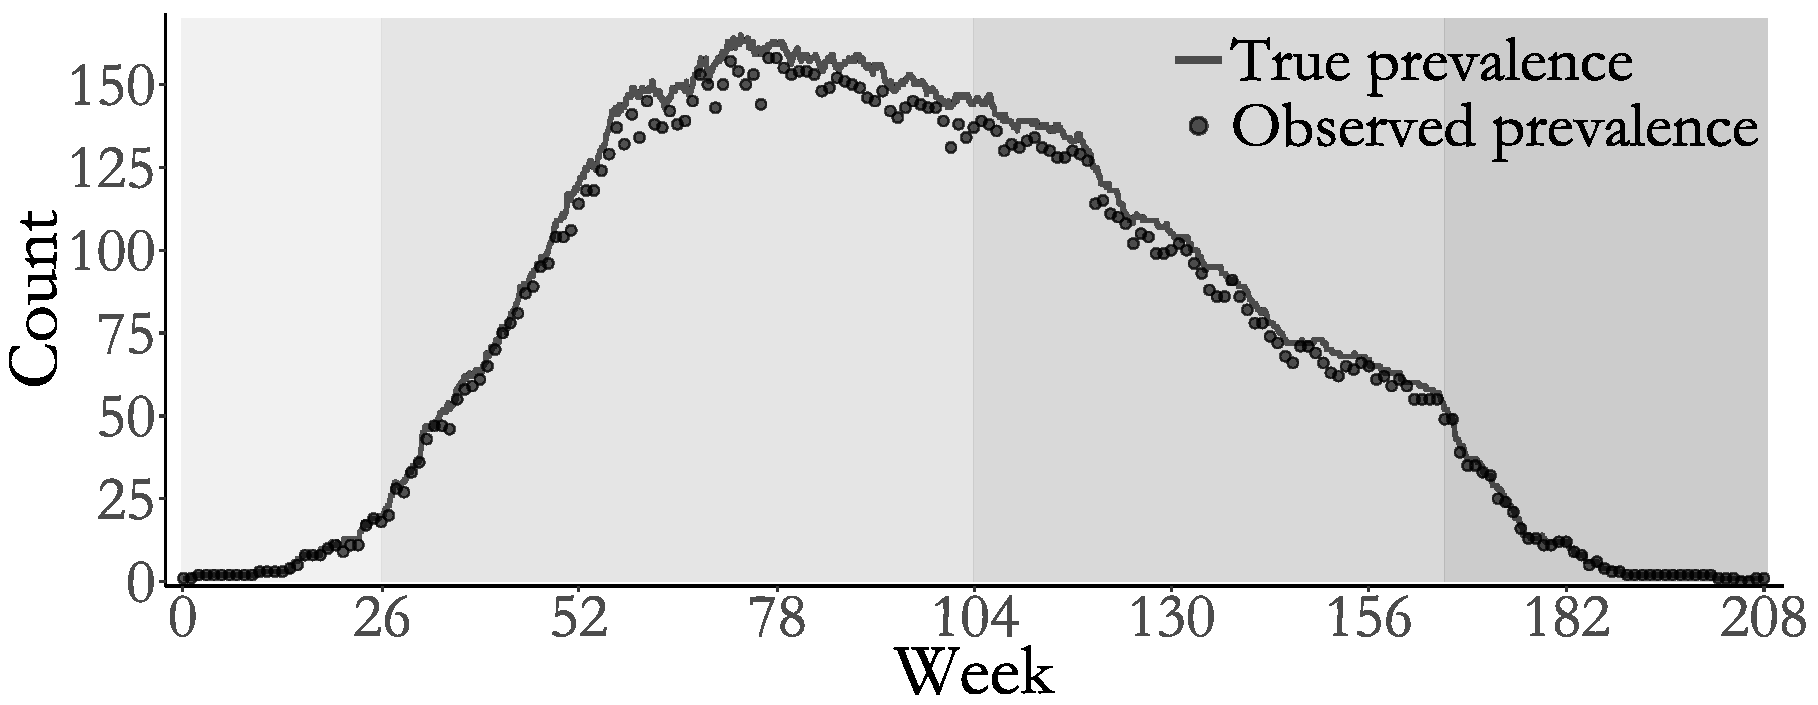
\includegraphics[width=0.5\linewidth]{figures/SEIR_misspec_data.pdf}
	\qquad
	\begin{tabular}[b]{lllll}
		& \multicolumn{4}{c}{Epoch}\\ \cmidrule{2-5}
		Parameter & 1 & 2 & 3 & 4 \\ \hline	
		$ R_0^{\mathrm{Eff}} $ & 14.9& 9.2& 0.1& 0\\
		$ 1/\gamma $ (days) & 210&210&90& 180\\
		$ 1/\mu $ (days) & 150 &330&300&70	\\
		&&&&
	\end{tabular}
	\captionsetup{labelformat=andtable}
	\caption[Simulated outbreak data from an SEIR model with time--varying dynamics.]{Simulated outbreak with SEIR dynamics that varied over four epochs (shaded regions). Weekly prevalence counts (points) were binomially sampled with sampling probability $ \rho = 0.95 $ from the true unobserved prevalence (solid line). The table presents the effective reproductive number computed based on the number of susceptibles at the beginning of each epoch, $ R_0^{\mathrm{Eff}} = \beta(\tau) S(\tau) / \mu(\tau) $, the mean latent period, $ 1/\gamma $, and the mean infectious period, $ 1/\mu $.}
	\label{fig:misspec_data}
\end{figure}

We fit SIR and SEIR models using our DA algorithm, and using PMMH with 2,500 particles, the paths for which were simulated approximately via $ \tau $--leaping with a time--step of 1 day. We assigned weakly informative priors for the rate parameters governing the epidemic dynamics in both models, and informative priors for the binomial sampling probability and the initial state probabilities (Table \ref{tab:misspec_priors}). MCMC chains for models fit via PMMH were plagued by particle degeneracy and did not converge (Figures \ref{fig:misspec_sir_bda_traceplots} and \ref{fig:misspec_seir_bda_traceplots}).

Both models fit via DA yield reasonable estimates for the within--subject disease dynamics (i.e., the infectious period, as well as the latent period in the case of the SEIR model). The posterior median average infectious period duration was estimated to be 292 days (95\% BCI: 263 days, 323 days) under SIR dynamics, and 287 days (95\% BCI: 260 days, 318 days) under SEIR dynamics. The posterior median average latent period under SEIR dynamics was 211 days (95\% BCI: 165 days, 260 days). The posterior median estimate of $ R_0 $ under SIR dynamics was 4.05 (95\% BCI: 3.40, 4.81), while under SEIR dynamics, the posterior median estimate of $ R_0 $ was 23.8 (95\% BCI: 15.1, 37.0). While the true prevalence fell well within the pointwise 95\% credible interval for both models (Figure \ref{fig:misspec_latent_posts}), we notice that the degree of model misspecification drastically affected our ability to estimate the history of the numbers of noninfectious people over the course of the epidemic. Under SIR dynamics, we drastically overestimate the number of susceptible individuals. The SEIR model much more closely resembles the time--varying SEIR model used to simulate the epidemic. Although the true path for the number of susceptible still falls outsize the 95\% credible interval at times, we are still able to reconstruct a reasonabe range of paths for the number of exposed individuals. This contrasts with the models fit in Section \ref{subsec:bda_sir_seir_sirs_sim}, which were not misspecified with respect to the true epidemic dynamics. In that case, the complete path of the epidemic fell well within the estimated credible intervals for all disease states for all three models (Figure \ref{fig:sim1_latent_post_all}). Therefore, we advise caution in  reconstructing the epidemic history for disease states that were not measured, particularly when severe model misspecification is suspected.

\begin{figure}[!h]
	\centering
	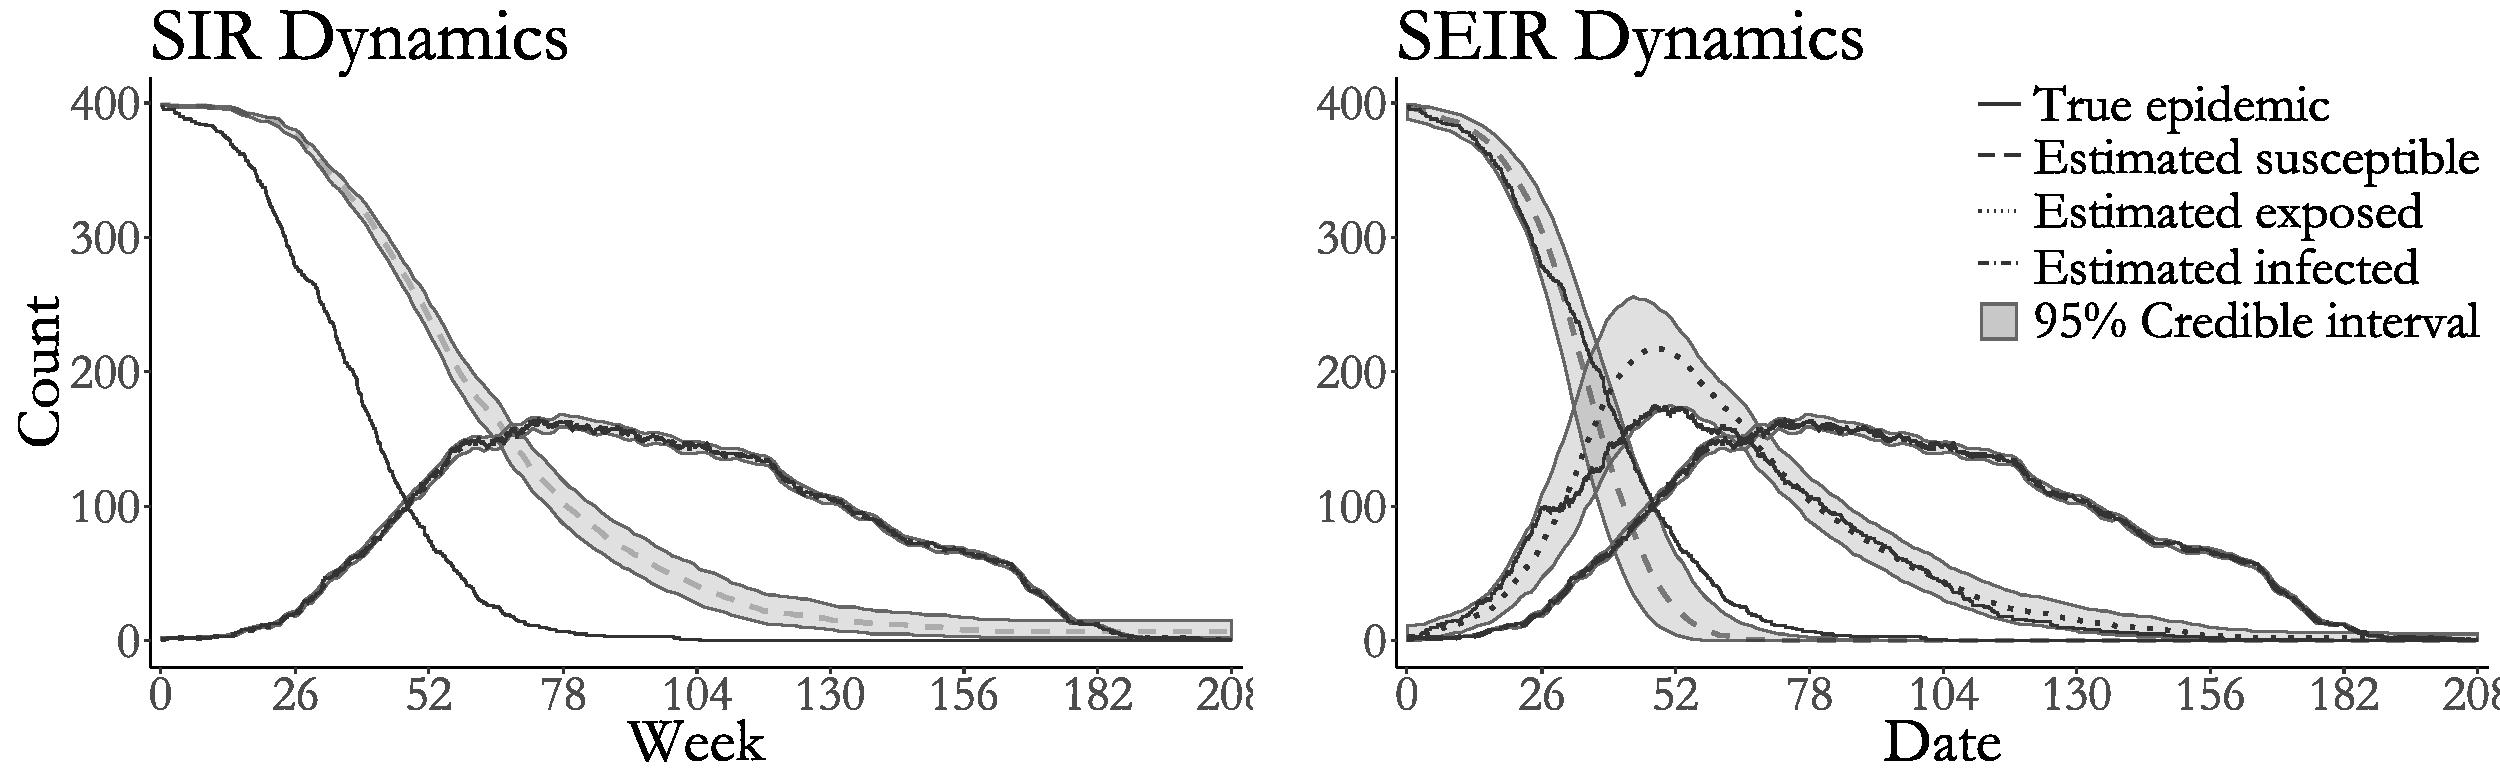
\includegraphics[width=0.9\linewidth]{figures/misspec_latent_posts.pdf}
	\caption[Latent posterior distributions for SIR and SEIR models fit to simulated data from an SEIR model with time--varying dynamics.]{True epidemic path (solid lines), pointwise posterior median estimate of the numbers of susceptibles (dashed line), exposed (dotted line), and infected individuals (dash--dotted line) and pointwise 95\% credible intervals (shaded regions) under SIR and SEIR dynamics.}
	\label{fig:misspec_latent_posts}
\end{figure}

\subsection{Effect of prior specification on posterior inference}
\label{subsec:prior_effect_sim}
Given the limited extent of aggregated prevalence counts, we must consider how our choices of prior distributions influence our posterior inferences. We simulated an outbreak with SIR dynamics in a population of 750 individuals for which $ R_0 = \beta \times 763 / \mu \approx 1.84 $ and the mean infectious period was $ 1/\mu = 7 $ days. We fit SIR models to binomially distributed weekly prevalence data, sampled with detection probability $ \rho = 0.2$, under the following four prior regimes: Regime 1 --- informative priors for all model parameters; Regime 2 --- vague priors for the rate parameters and an informative prior for the sampling probability; Regime 3 --- informative priors for the rate parameters and a flat prior for the sampling probability; Regime 4 --- vague priors for the rate parameters and a flat prior for the sampling probability. The same prior for the initial state probabilities was used in all four regimes. Complete simulation details and convergence diagnostics are supplied in Section \ref{sec:prior_effect_details}.

\begin{figure}[htbp]
	\centering
	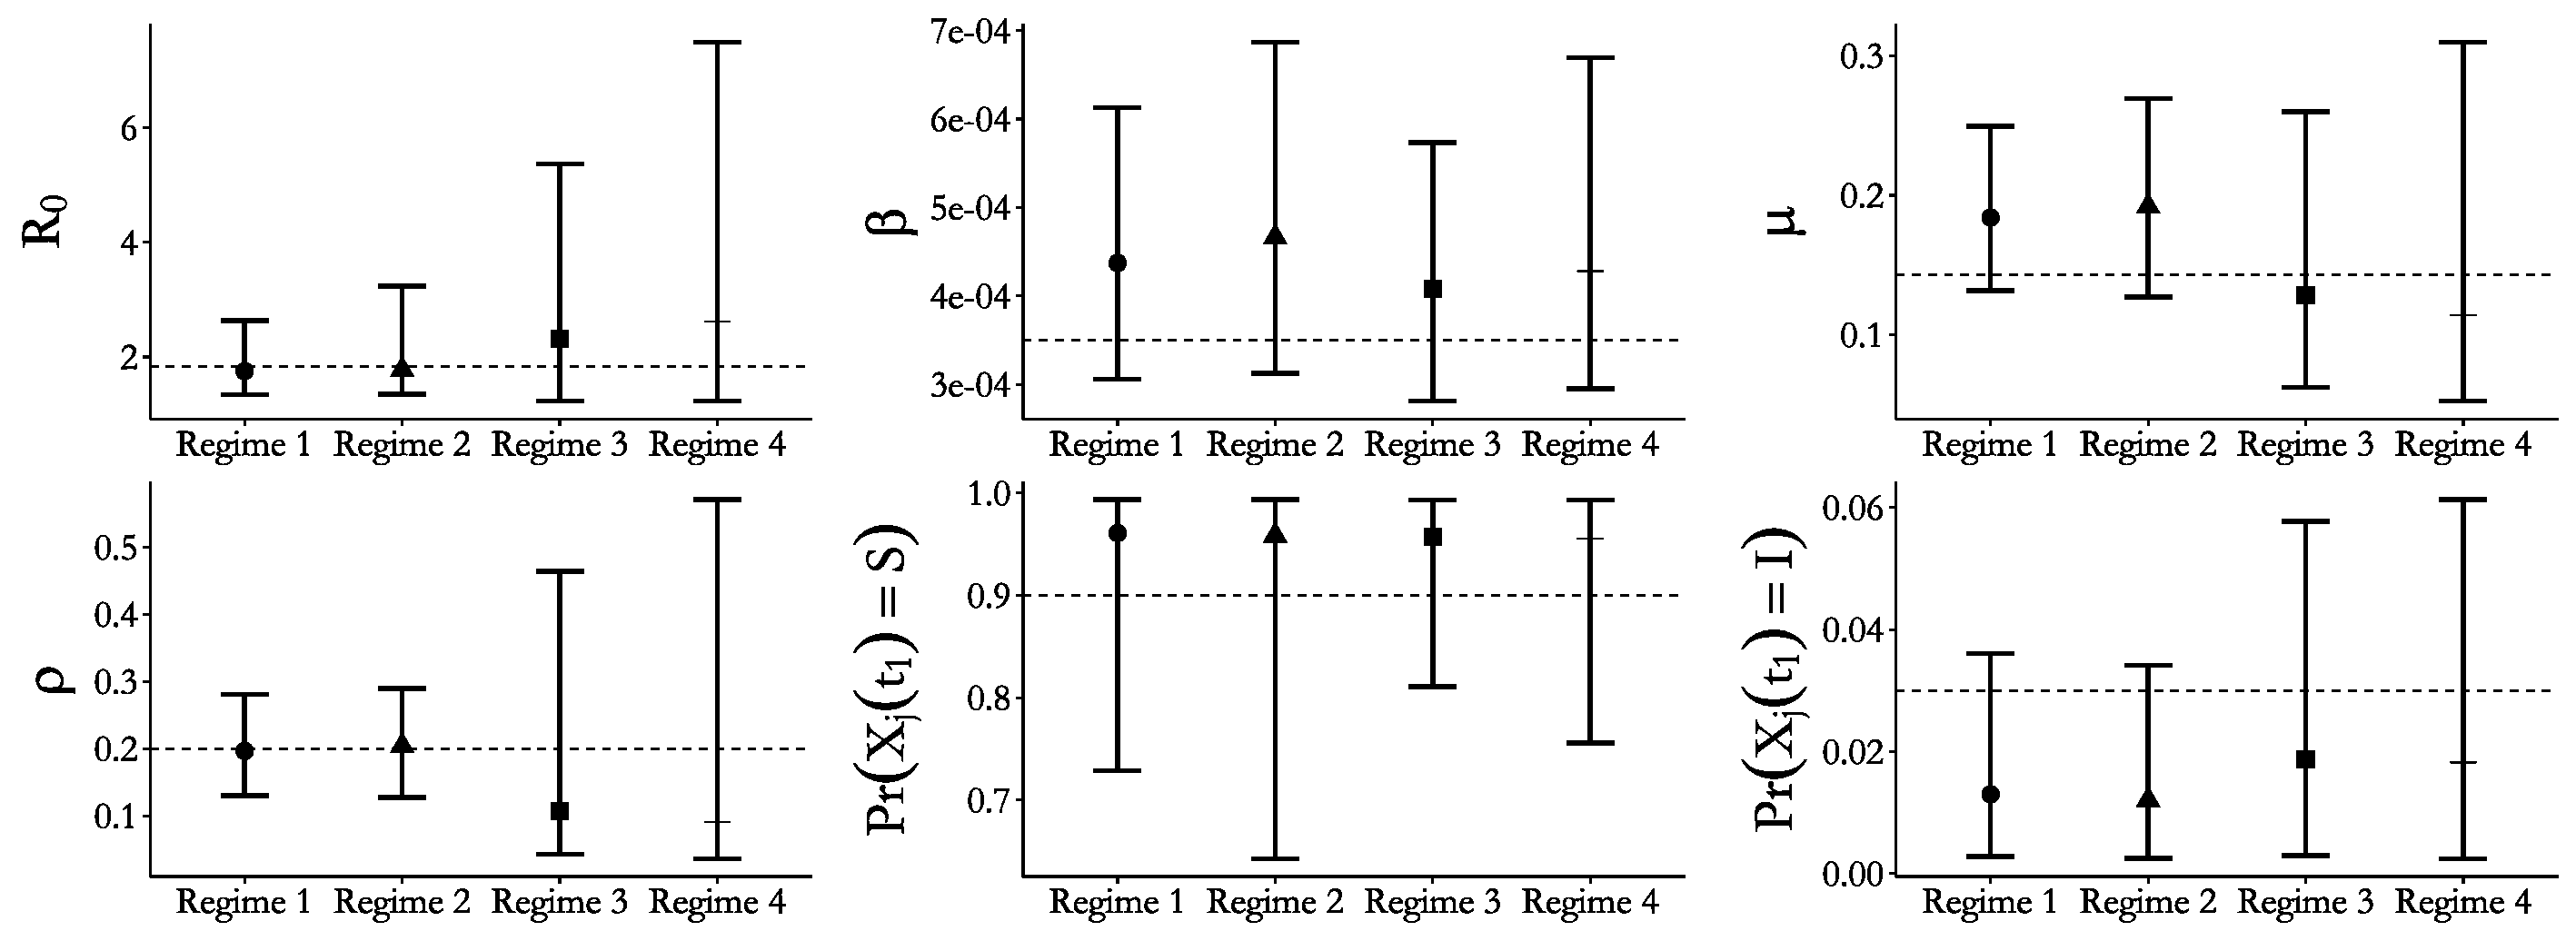
\includegraphics[width=\linewidth]{figures/prior_effect_credints.pdf}
	\caption[Posterior estimates of SIR model parameters under four prior regimes.]{Posterior median estimates and 95\% credible intervals for all SIR model parameters under four different prior regimes (Table \ref{tab:prior_effect_priors}). Regimes 1 and 3 set informative priors for the per--contact infectivity and recovery rates. Regimes 1 and 2 set informative priors for the binomial sampling probability. The same mildly informative prior for the initial state probabilities was used in all four regimes.}
	\label{fig:prior_credints}
\end{figure}

The true values for all model parameters fell within the 95\% credible intervals under all four prior regimes. Unsurprisingly, informative priors tended to result in narrower credible intervals for the parameters (Figure \ref{fig:prior_credints}) as well as for the latent process (Figure \ref{fig:prior_latent_posts}). The strength of prior information about the sampling probability affected the widths of credible intervals to a much greater extent than the priors for the rate parameters. Strong prior information about the sampling probability also resulted in substantially narrower credible intervals for disease prevalence under each of the prior regimes for the rate parameters. In contrast, informative priors for the rate parameters yielded only slightly narrower credible intervals for disease prevalence when holding constant the strength of the sampling probability prior. The effects on the initial state probability parameters seem to reverse this pattern, although we caution against overinterpretion given the paucity of data available for estimating those parameters. MCMC chains with strong priors for the binomial sampling probability also appeared to mix somewhat better than chains with diffuse priors for the sampling probabilty (see traceplots in Section \ref{sec:prior_effect_details}).

\begin{figure}[htbp]
	\centering
	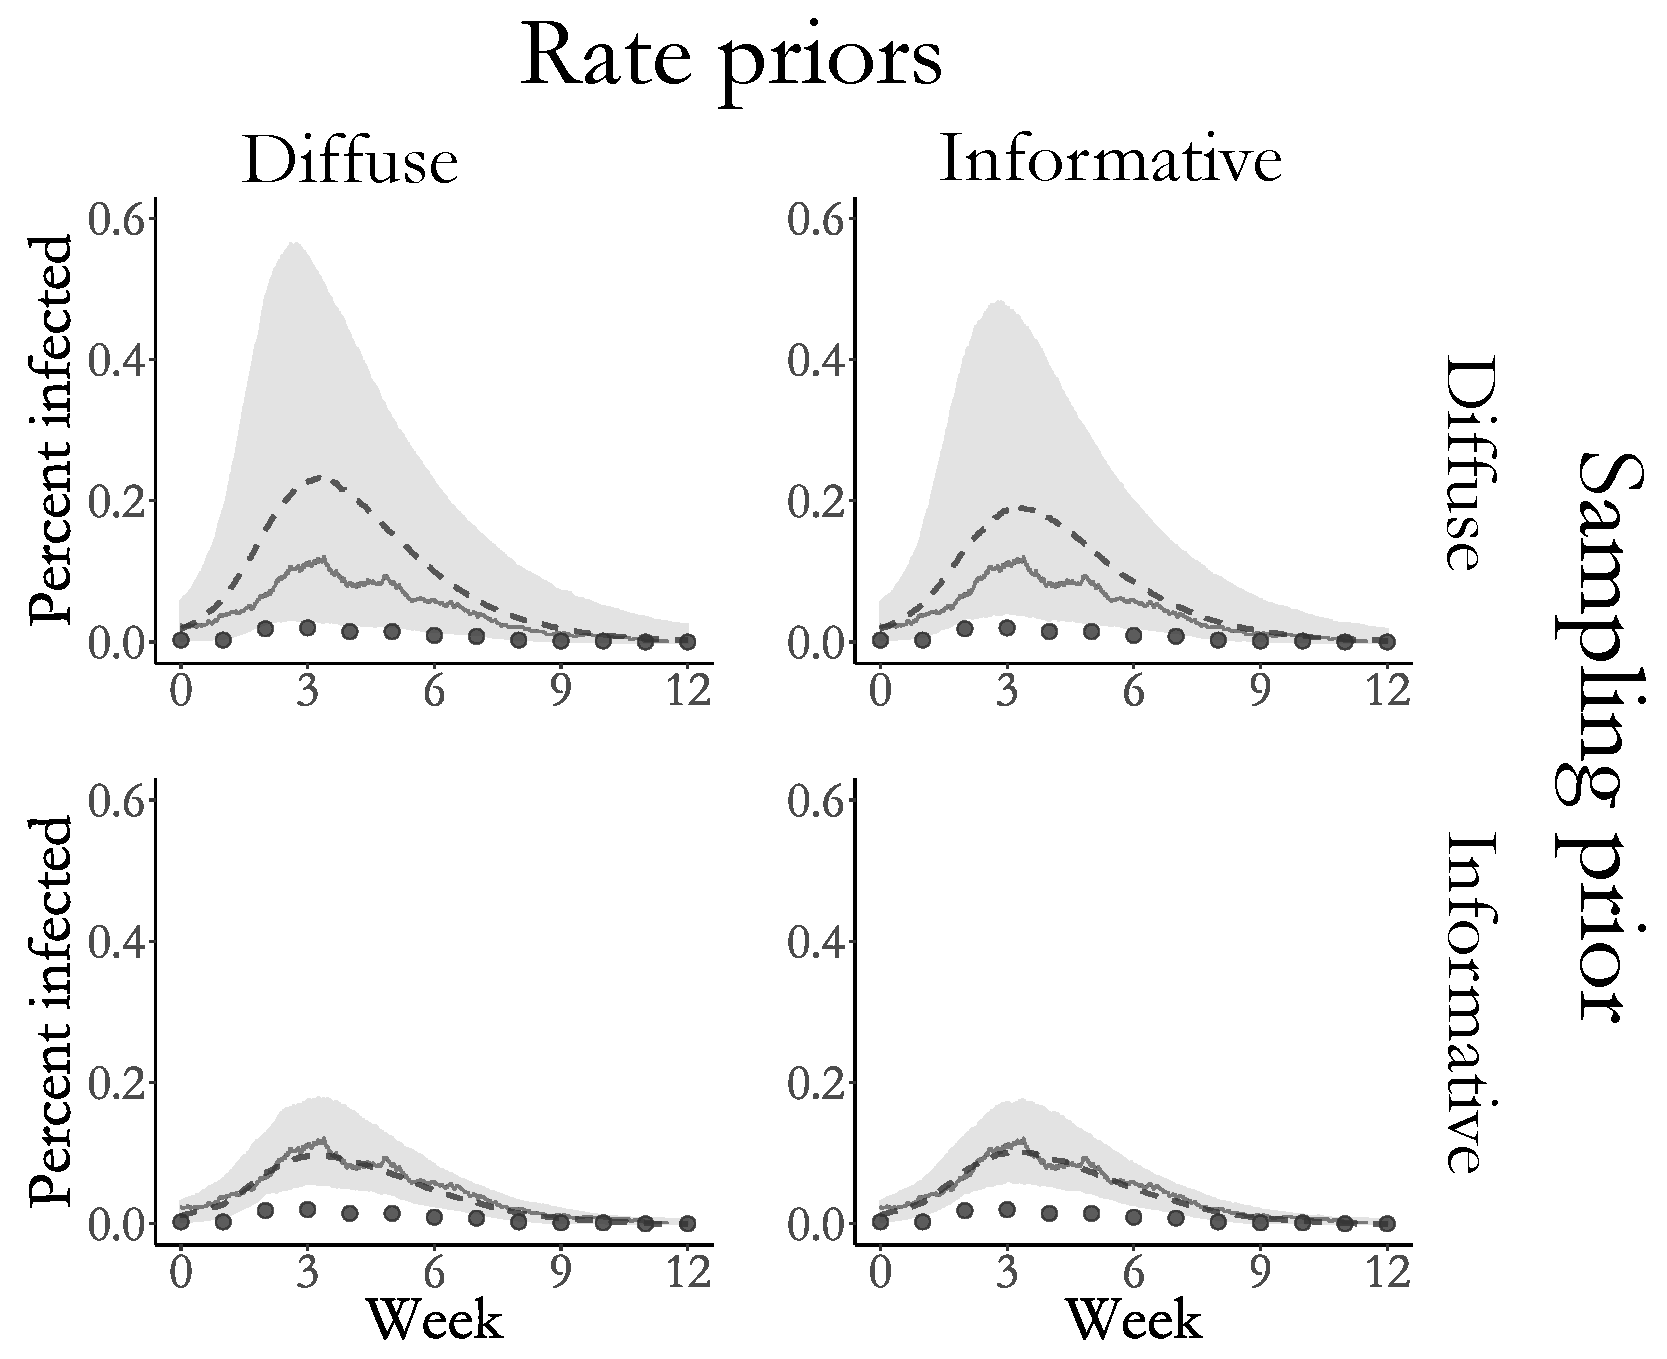
\includegraphics[width=0.6\linewidth]{figures/prior_latent_posts.pdf}
	\caption[Estimated latent posterior for an SIR model under four prior regimes.]{Estimated latent posterior distributions of disease prevalence in outbreaks simulated under four prior regimes for SIR model rate parameters and the binomial sampling probability. Depicted are the true unobserved prevalence (solid line), observed data (dots), pointwise posterior median prevalence (dashed line), and pointwise 95\% credible intervals (shaded region). Latent posterior estimates are based on a thinned sample, with every $250^{th}$ sample retained.}
	\label{fig:prior_latent_posts}
\end{figure}

\section{Example: Influenza in a British boarding school}
\label{sec:bda_bbs}

As an example, we apply the methods developed in this chapter data from the boarding school outbreak of influenza that was described in Section \ref{subsec:bbs_descrip}. We used our DA algorithm and PMMH to fit SIR and SEIR models with a binomial emission distribution to the data (see Section \ref{sec:bbs_supp} of the supplement for complete details). All of the parameters were assigned diffuse priors, which are plotted over the posterior ranges in Figure \ref{fig:bbs_densities}. The PMMH algorithm failed to converge for both models, which we suspect was due to a combination of model misspecification and the constrained state space of the binomial measurement process. We also fit a set of supplementary SIR and SEIR models in Section \ref{sec:bbs_neg_binom}, in which we assumed a negative--binomial emission distribution. This was done in order to facilitate comparison with PMMH, although we feel that a negative binomial emission distribution is not appropriate in such a closely monitored outbreak setting since it does not rule out over--reporting of cases.

\begin{figure}[ht!]
	\centering
	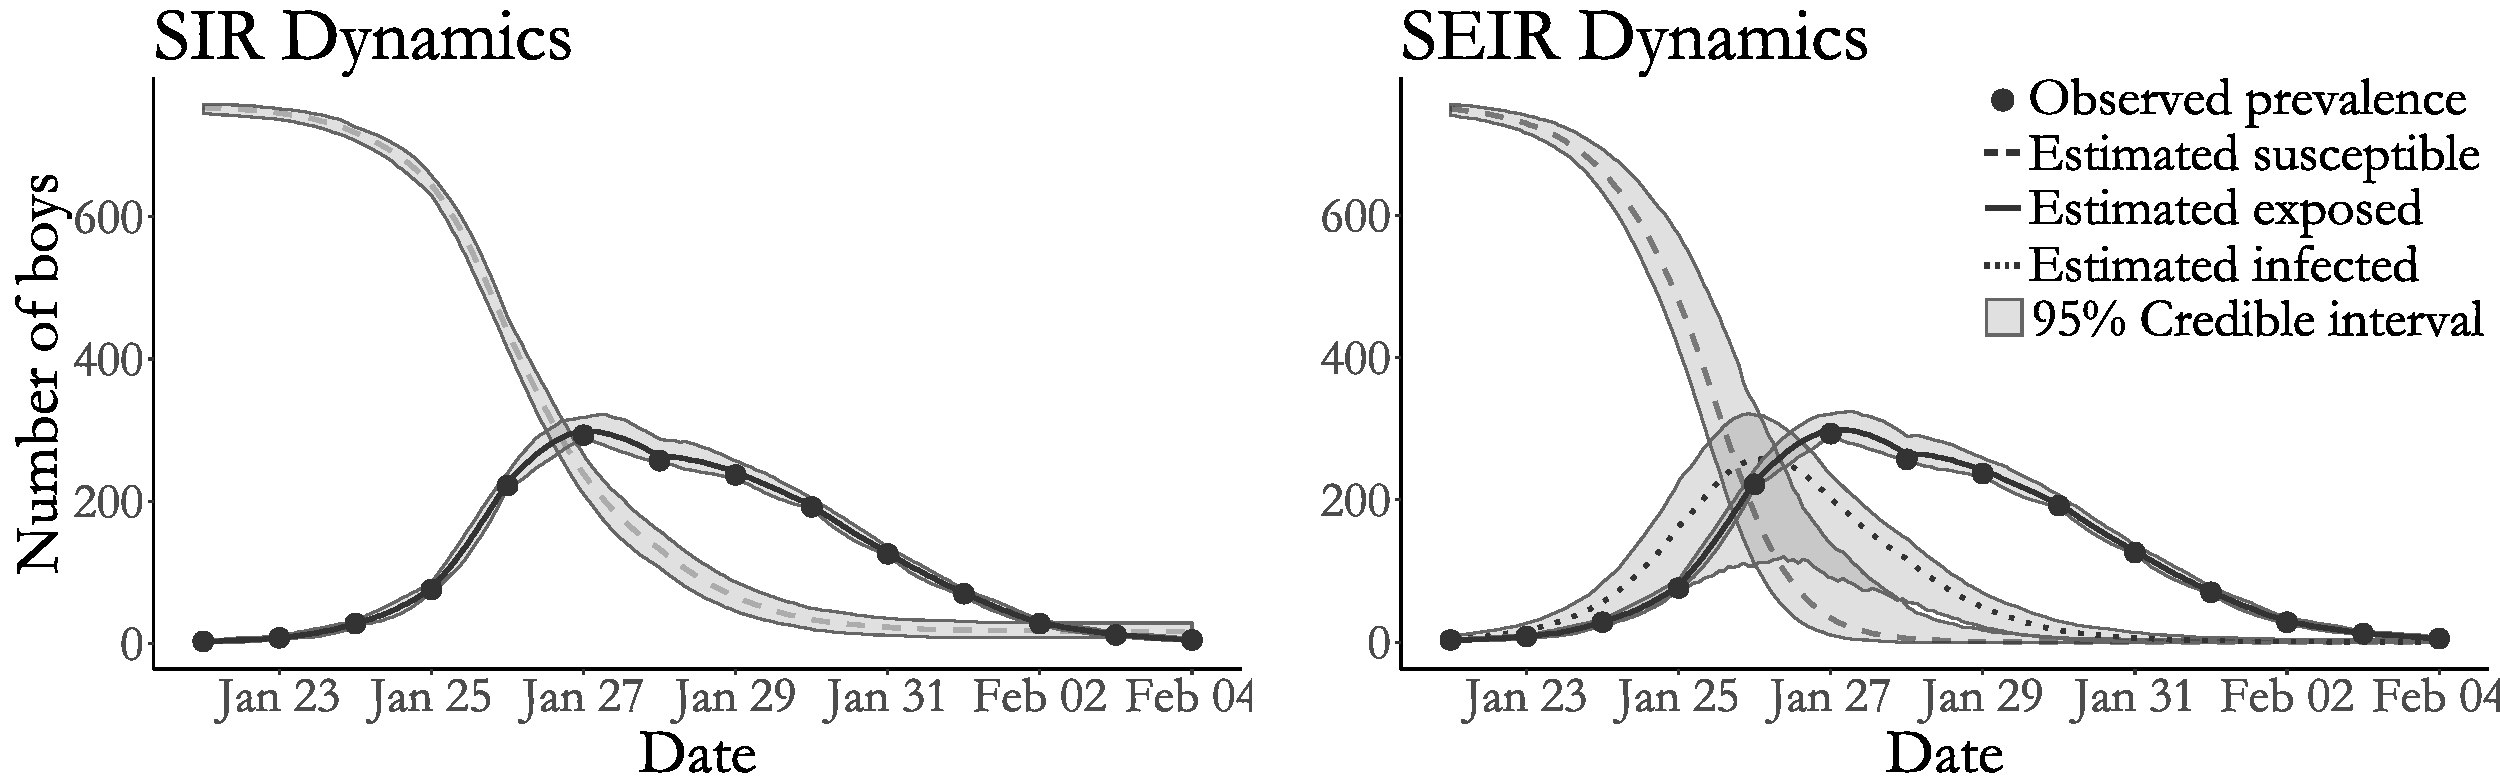
\includegraphics[width=\linewidth]{figures/bbs_latent_posts.pdf}
	\caption[Boarding school data and latent posterior under SIR and SEIR dynamics.]{Boarding school data, pointwise posterior median estimates and pointwise 95\% credible intervals (grey shaded areas) under SIR and SEIR dynamics of the numbers of susceptible boys (dashed line), exposed boys (dotted line), and infected boys (solid line). Posterior estimates based on a thinned sample, with every 250$ ^{th} $ configuration retained.}
	\label{fig:bbs_dat}
\end{figure}

Together, the SIR and SEIR models suggest that cases were detected with high probability and that the outbreak, though aggressive, was not atypical given the closed environment in which it occurred. The posterior median estimates of the detection probability, roughly 0.98 for both models (SIR 95\% BCI: 0.92, 1.00; SEIR 95\% BCI: 0.91, 1.00), suggested that while almost all of the infectious boys were detected, a handful of cases went unnoticed. The posterior median recovery rate under SIR dynamics corresponds to an average period of 2.16 days (95\% BCI: 1.99, 2.37) during which an infectious boy could transmit an infection to other boys before being confined to the infirmary. Under SEIR dynamics, the posterior median average infectious period was 2.12 days (95\% BCI: 1.95, 2.33), and the posterior median average latent period was 1.19 days (95\% BCI: 0.84, 1.51). These results are consistent with the typical progression of influenza, in which individuals typically incubate for between one to four days before symptoms manifest, and are typically infectious for one day before, and up to a week after, symptom onset \citep{cdcFlu}. The posterior median estimates of $ R_0 $ were 3.89 (95\% BCI: 3.40, 4.47) under SIR dynamics, and 10.38 (95\% BCI: 7.40, 14.11) under SEIR dynamics. Previous analyses of this dataset with trajectory matching estimate $ R_0 $ to be roughly 3.7 for the SIR model and 35.9 for the SEIR model \citep{wearing2005, keeling2008}, though we note that these estimates are based on deterministic models that do not properly account for distributional properties of the data. Another analysis using the linear noise approximation produced point estimates of $ R_0 $ in the range of 3.4--3.6, depending on the model specification \cite{ross2009parameter}. Our results for both models are also in agreement with estimates of SIR and SEIR model dynamics under a negative binomial emission distribution (see Section \ref{sec:bbs_neg_binom}).

\begin{figure}
	\centering
	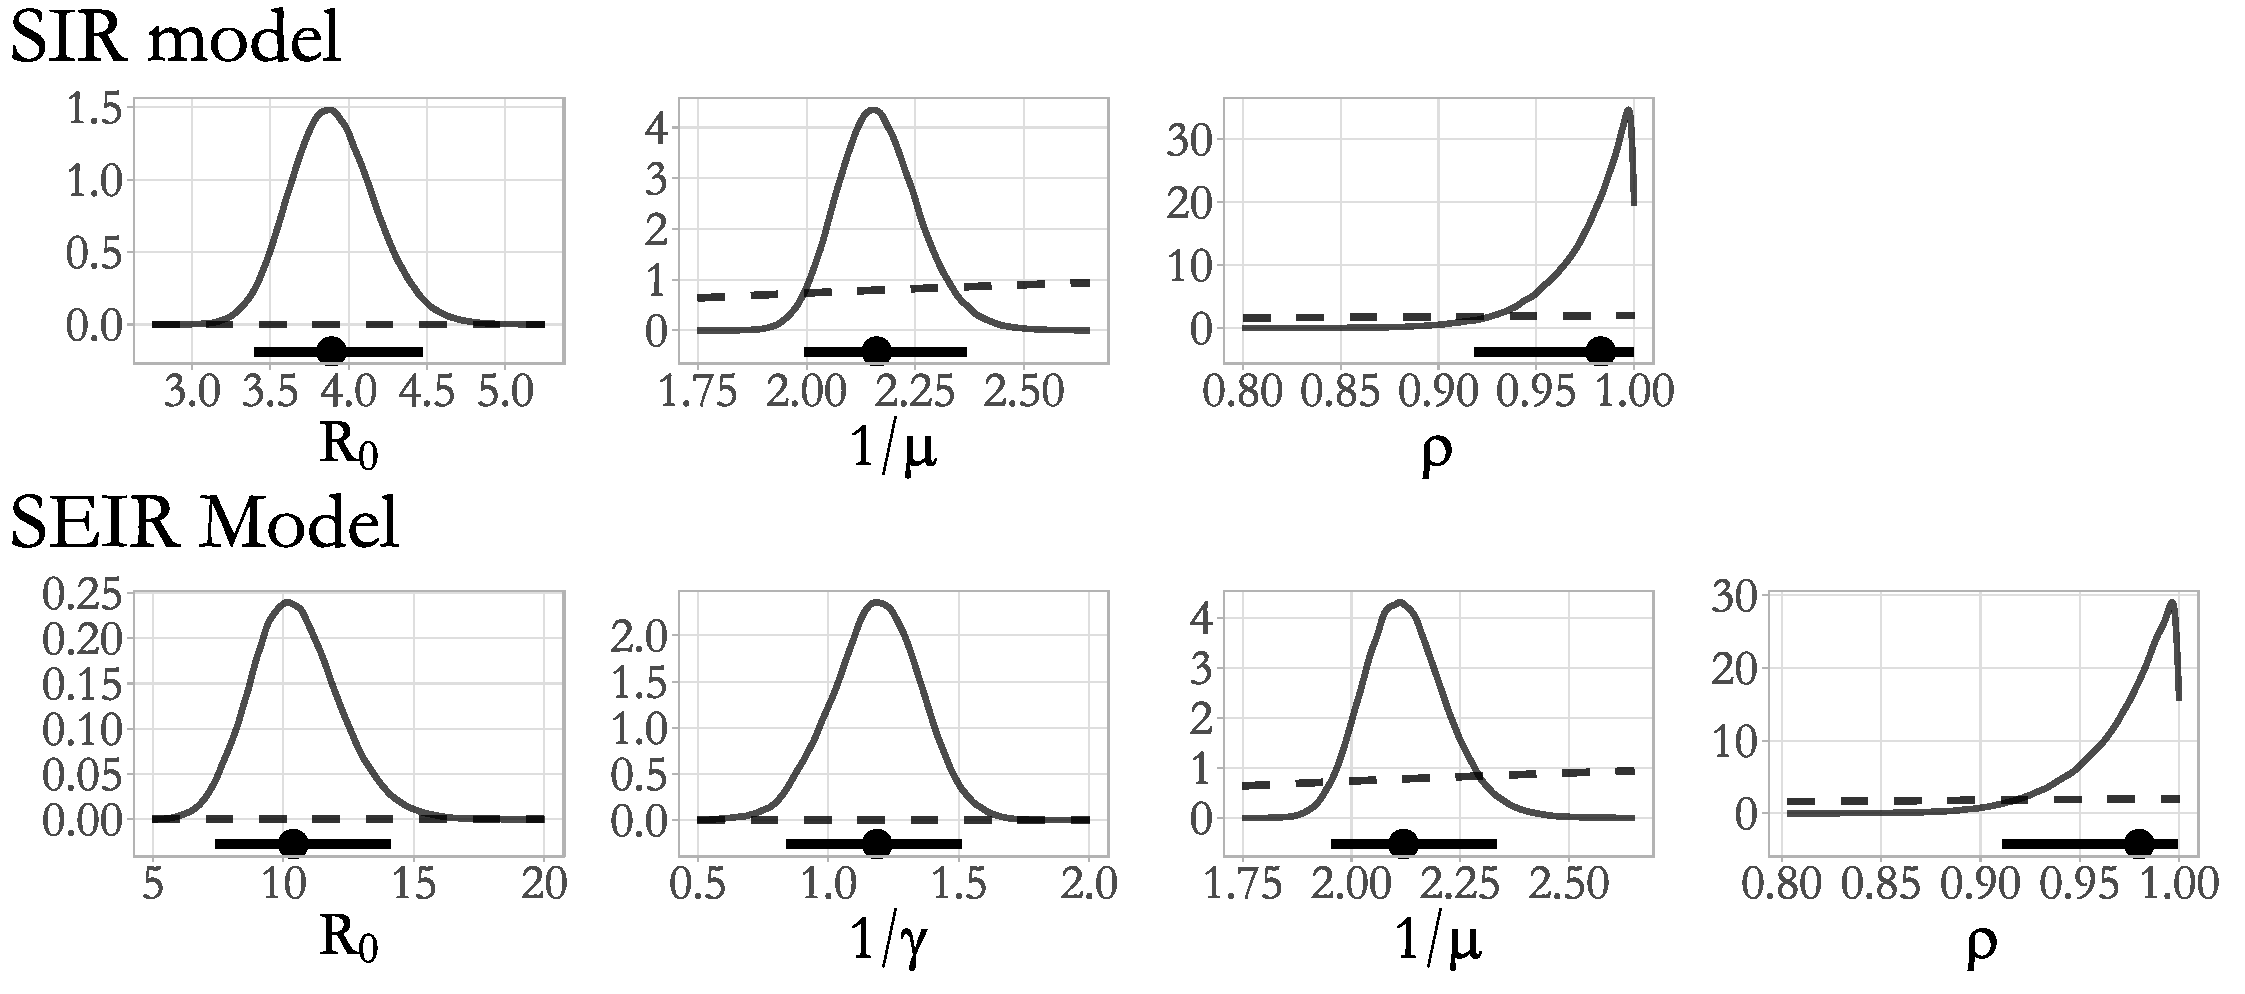
\includegraphics[width=0.95\linewidth]{figures/bbs_densities.pdf}
	\caption[Posterior estimates of SIR and SEIR model parameters fit to British boarding school outbreak data.]{Posterior density estimates for $ R_0 = \beta N /\mu $, the mean latent and infectious periods, $ 1/\gamma $ and $ 1/\mu $, and the binomial sampling probability, $ \rho $, from SIR and SEIR model parameters fit to the British boarding school data (solid lines). The posterior median and 95\% Bayesian credible intervals are drawn below the density plots (solid lines with circles). The implied prior densities (dashed lines) for $ R_0 $ and the latent and infectious periods, and the prior density for the binomial sampling probability, are plotted over the posterior ranges.}
	\label{fig:bbs_densities}
\end{figure}

\section{Discussion}
\label{sec:bda_discussion}

We have presented an agent--based Bayesian DA algorithm for fitting SEMs to disease prevalence time series counts. This was previously difficult, if not computationally infeasible, to carry out using traditional agent--based DA methods in the absence of subject--level data. Although we outlined the algorithm in the context of fitting an SIR model to binomially distributed prevalence data, our algorithm represents a general solution for fitting SEMs to prevalence counts. In simulations and the applied example, we fit SEIR and SIRS models to prevalence data, and in the supplement also fit SIR and SEIR models with a negative binomial emission distribution to the British boarding school data. We have demonstrated that our algorithm yields approximately valid inference when the population size is misspecified. Moreover, our algorithm is usable in settings where simulation--based methods, such as PMMH, break down due to misspecification of the SEM. Finally, our DA algorithm is carried out entirely at the subject level, making it possible to also incorporate subject--level covariates and household structure, or to fit models to subject--level data. 

There are two fundamental limitations of agent-based DA methods from which our algorithm is not excepted. First, the bookkeeping required to track the collection of subject--paths increases in size and complexity as the number of events grows large. Attempts to fit stochastic epidemic models in large populations using agent-based DA may be thwarted by prohibitive computational overhead. MCMC run times using our implementation, which was coded for reliability rather than speed, substantially degraded once the assumed population size was greater than a few thousand people. Second, we suspect that MCMC mixing in large populations could eventually become too slow for agent--based DA to be of practical use, even if solutions could be found for the computational bottlenecks. As the population size gets large, perturbations to the likelihood from re-sampling one subject at a time become relatively less significant. For this reason, we view extensions for jointly sampling multiple subject--paths as a critical step in mitigating slow MCMC mixing in large populations.

To conclude, we would like to comment on directions for future work that could be pursued. The DA algorithm in this paper addresses the problem of fitting SEMs to prevalence data. This type of data summarizes total number of infections in the population at a particular time. However, outbreak data often consist of incidence counts, which are the number of new cases accumulated in each inter-observation interval. Extending our DA algorithm to accommodate incidence data is an important next step and should be straightforward in situations where the state space for the subject level process is finite --- for instance, if a subject cannot become reinfected more than once or twice in a given inter-observation interval. Another line of inquiry involves improving the computational efficiency of the algorithm. One possibility would be to use a coarse grid for the time--varying force of infection used in each subject--path proposal, and to approximate the transition probabilities in the HMM step of the algorithm. For example, we could propose each subject--path conditionally on the disease states of all other subjects but assume that the force of infection is each inter--observation interval is fixed. This might lead to more subject--paths being rejected, but the loss could well be offset by not having to as many matrix exponentials. Finally, we note that the algorithm could also be used to fit semi--Markov models where transition probabilities depend on the duration of state occupancy. This would require a modification of the complete data likelihood and the Metropolis--Hastings ratio, though we could retain the Markovian structure of the proposal and possibly avoid costly rejected proposals by using a phase--type distribution to approximate the target semi--Markov process. % agent--based data augmentation
\chapter{Approximate Inference for Stochastic Epidemic Models of Outbreaks in Large Populations}
\label{chap:lna_for_sems}

\section{Overview}
\label{sec:lna_overview}

Surveillance and outbreak response systems often report incidence counts of new cases detected in each inter--observation time interval. Analyzing this type of time series data is challenging since we must overcome many of the same challenges that we face in modeling the transmission dynamics of infectious diseases in small population settings with prevalence data --- discrete snapshots of a continuously evolving epidemic process, detecting a fraction of the new cases, and often directly observing only one aspect of the disease process. Furthermore, our task is made more difficult by the additional computational burden that results from repeated evaluation of CTMC likelihoods; the products of exponential waiting time distributions consist of polynomially increasing numbers of terms, and agent--based data augmentation (DA) MCMC algorithms become unwieldy as the numbers of subject--path proposals required to meaningfully perturb the CTMC likelihood get large \citep{fintzi2017efficient}. 

In this chapter, we show how the LNA of Section \ref{subsubsec:lna_background} can be adapted to obtain approximate inference for SEMs fit to epidemic count data in large populations. Our contributions are threefold: First, we demonstrate how the SEM dynamics should be reparameterized so that the LNA can be used to approximate transition densities of the counting processes for disease state transition events. Second, we fold the LNA into a Bayesian DA framework in which latent LNA paths are sampled using the elliptical slice sampling (EliptSS) algorithm of \cite{murray2010}. This provides us with general machinery for jointly updating the latent paths while absolving us of the \textit{de facto} requirement that the emission probability distribution to be Gaussian in order to preserve computational efficiency as in \cite{fearnhead2014,komorowski2009}, lest we resort to computationally intensive particle filter methods for non--Gaussian emission distributions as in \cite{golightly2015delayed}. Finally, we introduce a non--centered parameterization (NCP) for the LNA that massively improves the efficiency of our DA MCMC framework and makes it tractable for fitting complex models. 

\section{Fitting Stochastic Epidemic Models via the Linear Noise Approximation}
\label{sec:lna_methods}

For clarity, we will present the algorithm for fitting SEMs via the LNA in the context of fitting the susceptible--infected--recovered (SIR) model to negative binomial distributed incidence counts. We will, however, provide notation where appropriate so that the generality of the algorithm should be apparent. The SIR model is an abstraction of the transmission dynamics of an outbreak as a closed, homogeneously mixing population of $ N $ exchangeable individuals who are either susceptible $ (S) $, infected, and hence infectious, $ (I) $, or recovered $ (R) $. It is important to note that the model compartments refer to disease states as they relate to the transmission dynamics, not the disease process. Thus, an individual is considered to be recovered when she no longer has infectious contact with other individuals in the population, not when she clears disease carriage. As another example, in the susceptible--exposed--infected--recovered (SEIR) type models that we will consider later, the latent period in which an individual is exposed, but not yet infectious, should be understood as possibly varying in population with different contact dynamics, even when the incubation period of the pathogen should arguably be consistent across groups.

\subsection{Measurement Process and Data}
\label{subsec:lna_measproc}
Incidence data, $ \bY = \lbrace Y_1,\dots,Y_L\rbrace $,  arise as increments of the numbers of new cases accumulated in a set of time intervals, $ \mcI = \lbrace\mcI_1,\dots,\mcI_L:\ \mcI_\ell = (t_{\ell-1},t_\ell]\rbrace $. In outbreak or surveillance settings, we do not typically believe that every case is detected since individuals may be asymptomatic or may escape detection. Let $ \bN^c = (N^c_{SI}, N^c_{IR}) $ denote the counting process for the cumulative numbers of infections ($ S\rightarrow I $ transitions) and recoveries ($ I\rightarrow R $ transitions), and let $ \Delta \bN^c(t_\ell) = \bN^c(t_\ell) - \bN^c(t_{\ell-1})$ denote the change in cumulative numbers of transitions over $ \mcI_\ell $; so, $ \Delta N^c_{SI}(t_\ell)$ is the incidence over $ (t_{\ell-1},t_\ell] $. We might choose to model the number of observed cases as a negative binomial sample of the true incidence with detection rate $ \rho $ and over--dispersion parameter $ \phi $. Thus,
\begin{equation}
\label{eqn:incidence_emitprob}
Y_\ell|\Delta N^c_{SI}(t_\ell),\rho \sim \mr{Neg.Binom.}(\mr{\mu} = \rho\Delta N^c_{SI}(t_\ell),\ \sigma^2 = \mu + \mu^2/\phi).
\end{equation}

There are two minor points that we wish to make before proceeding. First, we have allowed for the possibility that cases are over--reported. This is not a necessary assumption for any of the subsequent results. It is also not unreasonable when studying outbreaks in large populations where the ``fog of war" might lead to inflation of reported incidence or misclassification of individuals whose symptoms are similar to the disease of interest. Allowing for the possibility of over--reporting is also not particularly problematic when the detection probability is low since the emission densities will have negligible mass above the true incidence. The second point is that we are making this modeling choice with an eye on the compatibility of the emission distribution with the eventual LNA approximation, which takes real, not integer, values. The negative binomial distribution is well defined for non--integer values of its mean parameter. 

\subsection{Latent Epidemic Process}
\label{subsec:lna_epid_proc}

The SIR model is often expressed in terms of compartment counts, $ \bX^c = \lbrace S^c,I^c,R^c\rbrace $, that evolve in continuous time on state space $ \mcS_X^c = \left \lbrace \mcC_{lmn}:l,m,n\in\lbrace0,\dots,N\rbrace,\ l+m+n=P\right \rbrace $. We will make the (not particularly limiting) modeling choice to express the waiting times between disease state transitions as being exponentially distributed. Thus, $ \bX $ evolves according to a Markov jump process (MJP). If our data had consisted of prevalence counts, which arise as partial observations of infected individuals, we might have chosen to approximate transition densities of the MJP for $ \bX $ in the usual way that appears in \cite{komorowski2009,fearnhead2014}. 

However, incidence data are discretely observed, partial realizations of the increments of counting processes that evolve continuously in time as individuals transition among disease states. The emission probabilities for incidence data, e.g., (\ref{eqn:incidence_emitprob}), depend on the change in $ N_{SI}^c $ over the time interval $ (t_{\ell-1},t_\ell] $, not on the change in $ I $ over the interval. It would be incorrect to treat incidence as simply the difference in prevalence. We could easily conjure up a scenario where there are positive numbers of infections, but where the prevalence, discretely observed, does not appear to change due to an equal number of recoveries. We need to construct the LNA that approximates transition densities of $ \bN $ if we are to write down correctly specified emission probabilities.

The cumulative incidence process for infections and recoveries, $ \bN^c $, is a Markov jump process with state space $ \mcS_N^c = \left \lbrace \mcC_{jk}:j,k\in\lbrace0,\dots,N\rbrace\right \rbrace $. Let $ \beta $ denote the per--contact infection rate, and $ \mu $ denote the rate at which each infected individual recovers. The rate at which $ \bN^c $ transitions from state $ \bn $ to $ \bn^{\prime}$ is 
\begin{equation}
	\label{eqn:lna_sir_rates}
	\blambda_{\bn,\bn^\prime} = \left \lbrace \begin{array}{ll}
	\lambda_{SI} = \beta S I, & \bn = (n_{SI},n_{IR}),\ \bn^\prime = (n_{SI}+1,n_{IR}),\text{ and } n_{SI}+1\leq P, \\
	 \lambda_{IR} = \mu I, &  \bn = (n_{SI},n_{IR}),\  \bn^\prime = (n_{SI},n_{IR}+1),\text{ and } n_{IR}+1\leq P, \\
	 0, & \text{for all other } \bn \text{ and } \bn^\prime.
	\end{array} \right.
\end{equation}

\subsection{Tractable Approximations for Intractable Likelihoods}
\label{subsec:lna_motivation}
We would like to make inferences about the posterior distribution of the parameters, e.g., $ \btheta = (\beta, \mu, \bX_0, \rho)$, that govern the latent epidemic process and sampling distribution, 
\begin{align}
\label{eqn:intractable_posterior}
 \pi(\btheta|\bY)&\propto \pi(\bY|\btheta)\pi(\btheta) = \int L(\bY|\bN^c,\btheta)\pi(\bN^c|\btheta)\pi(\btheta)\rmd\pi(\bN^c)\nonumber\\
 &= \int_{\mcS^c}\prod_{\ell=1}^L \Pr\left (\bY_\ell|\Delta\bN_{SI}^c(t_\ell),\btheta\right )\pi\left (\bN^c(t_\ell)|\bn^c(t_{\ell-1}),\btheta\right )\pi(\btheta)\rmd\pi(\bN^c)
\end{align}
where $ \pi(\btheta) $ specifies the prior density of the model parameters. However, this integral is analytically intractable and is challenging to compute numerically due to the size of the state space of $ \bN^c $. In the following subsections, we will obtain the LNA for transition densities of $ \bN^c $, turning (\ref{eqn:intractable_posterior}) into an integral over a much more computationally tractable product of Gaussian densities and non--Gaussian emission probabilities. As we shall see, approximating the complete data likelihood in the posterior $ \pi(\btheta,\bN^c|\btheta) $ with a Gaussian state space model will facilitate the use of efficient algorithms for sampling from the approximate posterior. 

\subsection{Diffusion Approximation}
\label{subsec:diff_approx}

As outlined in Section \ref{subsubsec:diff_approx}, there are a variety of methods for arriving at a diffusion approximation for a Markov jump process, which under certain conditions yield equivalent results (for a comprehensive reference, see \cite{fuchs2013inference}). In the interest of clarity, we follow \cite{fearnhead2014,golightly2013simulation,golightly2015delayed,wilkinson2011stochastic} and appeal to an intuitive, though somewhat informal, construction of the CLE by matching its drift and diffusion with the approximate moments of increments of the MJP path in infinitesimal time intervals. For more detailed presentations see \cite{fuchs2013inference,gillespie2000chemical,wallace2012linear}. 

Suppose that, at the current time, the compartment counts are given by $ \bX^c(t) = \bx^c_t $. We are interested in approximating the numbers of infections and recoveries in a small time interval, $ (t, t+\dt] $, i.e., $ \bN^c(t+\dt) - \bN(t)$. Now, suppose that we can choose $ \dt $ such that the following two \textit{leap} conditions hold:

\begin{enumerate}
	\item $ \dt $ is sufficiently \textit{small} that the $ \bX^c $ is essentially unchanged over $ (t,t+\dt] $, so that the rates of infections and recoveries are approximately constant: 
	\begin{equation}\label{eqn:tau_cond_1}
	\blambda(\bX^c(t^\prime)) \approx \blambda(\bx^c(t)),\ \forall t^\prime \in (t,t+\dt].
	\end{equation}
	\item $ \dt $ is sufficiently \textit{large} that we can expect many disease state transitions of each type:
	\begin{equation}\label{eqn:tau_cond_2}
	\blambda(\bx^c(t)) \gg \bs{1}.
	\end{equation}
\end{enumerate}

Condition (\ref{eqn:tau_cond_1}), which can be trivially satisfied just by choosing $ \dt $ to be infinitesimally small, implies that the numbers of infections and recoveries in $ (t,t+\dt] $ are essentially independent of one another since the rates at which they occur are approximately constant within the interval \cite{gillespie2000chemical}. This condition also carries the stronger implication that the numbers of infections and recoveries in the interval are independent Poisson random variables with rates $ \blambda(\bx^c(t)\dt) $, i.e., $ N^c_{SI}(\dt) \sim \mr{Poisson}(\beta S(t)I(t)\dt) $ and $ N^c_{IR}(t+\dt) \sim \mr{Poisson}(\mu I(t)\dt) $. Condition (\ref{eqn:tau_cond_2}), which we can reasonably expect to be satisfied in large populations where transmission dynamics are near their deterministic ODE limits \cite{wallace2012linear}, implies that the Poisson distributed increments can be well approximated by independent Gaussian random variables. 

When (\ref{eqn:tau_cond_1}) and (\ref{eqn:tau_cond_2}) are satisfied, we can approximate the integer--valued processes, $ \bX^c $ and $ \bN^c $, with the real--valued processes, $ \bX $ and $ \bN $. For the SIR model, the state space of $ \bX $ is $ \mcS_X^R = \lbrace \mcV_{lmn}:l,m,n \in [0,N],\ l+m+n=P\rbrace $, and the state space  of $ \bN $ is $ \mcS_N^R = \lbrace \mcV_{jk}: j,k \in [0,N],\ j\geq k \rbrace $. More generally, the state space of $ \bX $ will be the set of compartment volumes that are non--negative and that sum to the population size, while the state space of $ \bN $ is the set of non--decreasing and non--negative incidence paths, constrained so that they do not lead to invalid prevalence paths (e.g., if at some point there are more recoveries than infections, which would lead to a negative number of infected individuals). For now, we will ignore the constraints on $ \mcS_N^R $ and $ \mcS_X^R $, and approximate the changes in cumulative incidence of infections and recoveries in an infinitesimal time step as 
\begin{equation}
\bN(t+\dt) - \bN(t) \approx \blambda(\bX(t))\dt + \bLambda(\bX(t))^{1/2}\dt^{1/2}\bZ,
\end{equation}
where $ \bLambda = \diag\left (\blambda(\bX) \right )$ and $ \bZ\sim MVN(\bs{0},\mb{I}) $. This implies the equivalent CLE,
\begin{equation}
\label{eqn:sir_cle_X}
\rmd \bN(t) = \blambda(\bX(t))\dt + \bLambda(\bX(t))^{1/2}\rmd\bW_t, 
\end{equation}
where $ \bW_t $ is a vector of independent Brownian motion and $ \bLambda(\bX(t))^{1/2} $ denotes the matrix square root of $ \bLambda(\bX(t)) $. 

\subsubsection{Reparameterizating the CLE in terms of incidence}
\label{subsubsec:cle_repar}
The LNA of (\ref{eqn:sir_cle_X}) will involve derivatives of the rates, $ \blambda $, with respect to the incidence process, $ \bN $. In order to enable us to compute these derivatives, we borrow from \cite{breto2011compound,ho2016direct} a reparameterization for $ \bX (t)$ in terms of $ \bN(t) $, conditional on the initial conditions $ \bX(t) = \bX_0 $ and $ \bN(t) = \bs{0} $. Let $ \bA $ denote the matrix whose rows specify changes in counts of susceptible, infected, and recovered individuals corresponding to one infection or recovery event:
\begin{equation}
\label{eqn:sir_stoich}
\bA = \kbordermatrix{& S & I &  R\\
	S\rightarrow I& -1& 1 & 0\\
	I \rightarrow R & 0& -1 & 1
}.
\end{equation}

Now, $ \bX $ is coupled to $ \bN $ via the relationship,
\begin{equation}
\label{eqn:incid2prev}
\bX(t) = \bX_0 + \bA^T\bN(t).
\end{equation}
For the SIR model, 
\begin{align}
\left (\begin{array}{c}
S(t) \\
I(t) \\
R(t)
\end{array}\right ) &= \left (\begin{array}{c}
S_0 - N_{SI}(t) \\
I_0 + N_{SI}(t) - N_{IR}(t) \\
R_0 + N_{IR}(t)
\end{array}\right ),
\end{align}
which enables us to rewrite (\ref{eqn:sir_cle_X}) as
\begin{align}
\label{eqn:sir_cle_N}
 \rmd\bN(t)&= \blambda(\bN(t))\dt + \bLambda(\bN(t))^{1/2}\rmd\bW_t \\
 &= \left (\begin{array}{cc}
\beta (S_0 - N_{SI}(t))(I_0 + N_{SI}(t) - N_{IR}(t))\\
\mu(I_0 + N_{IR}(t))\dt 
\end{array}\right )\dt + \nonumber\\
&\hspace{0.5in}\left(\begin{array}{cc}
\beta (S_0 - N_{SI}(t))(I_0 + N_{SI}(t) - N_{IR}(t)) & 0 \\
0 & \mu(I_0 + N_{IR}(t))
\end{array}\right)^{1/2}\rmd\bW_t. \nonumber 
\end{align}

\subsubsection{Log transforming the CLE}
\label{subsubsec:log_cle}
Changes in compartment volumes affect the rates, and hence increments in the incidence process, multiplicatively. Therefore, from a scientific perspective, we would like for perturbations about the drift in (\ref{eqn:sir_cle_N}) to be symmetric on a multiplicative, not an additive scale. Hence, we log transform (\ref{eqn:sir_cle_N}). Let $ \bNtil = \log(\bN + \bs{1}) \implies\bN = \exp(\bNtil) - \bs{1}$. By It\^{o}'s lemma \cite{oksendal2003stochastic}, the corresponding SDE for $ \bNtil $ is 
	\begin{align}
\label{eqn:sir_log_cle}
\rmd\bNtil(t) &= \diag\left (\exp(-\bNtil(t)) - 0.5\exp(-2\bNtil(t))\right )\blambda\left (\exp(\bNtil(t))-\bs{1}\right )\dt\ + \nonumber\\
& \hspace{0.5in} \diag\left (\exp(-\bNtil(t))\right )\bLambda\left (\exp(\bNtil(t))-1\right )^{1/2}\rmd\bW_t \\
\label{eqn:sir_log_cle_gen}
&= \boeta(\bNtil(t))\dt + \bPhi(\bNtil(t))^{1/2}\rmd\bW_t
\end{align}

\subsection{Linear Noise Approximation}
\label{subsec:sir_lna}

In Section \ref{subsubsec:lna_background}, we followed \cite{fearnhead2014,golightly2013simulation,golightly2015delayed} in obtaining the LNA for SDEs of the same form as (\ref{eqn:sir_log_cle_gen}). Briefly, the derivation proceeded as follows: we first decomposed $ \bNtil $ into its deterministic ODE limit and a stochastic residual. The SDE corresponding to (\ref{eqn:sir_log_cle}) was then Taylor expanded around its deterministic limit, discarding higher order terms, to obtain a linear SDE for the residual. This linear SDE had an explicit solution as a Gaussian random variable. As noted in \cite{wallace2012linear}, the LNA can reasonably approximate the stochastic aspects of a density dependent MJP when conditions (\ref{eqn:tau_cond_1}) and (\ref{eqn:tau_cond_2}) are satisfied, at least over short time horizons. Over longer time periods the approximation may deteriorate as departures from the deterministic behavior of the system, which is determined by its initial conditions, accumulate.  One solution, proposed in \cite{fearnhead2014} and that we will adopt here, is to restart the LNA approximation at the beginning of each inter--observation interval. 

The restarting LNA of (\ref{eqn:sir_log_cle_gen}) over a time interval, $ (t_{\ell-1},t_\ell] $, was seen to be a Gaussian approximation of the transition density of $ \bNtil $,
\begin{equation}
\label{eqn:lna_transition_density}
\bNtil(t_\ell)|\bntil(t_{\ell-1}), \bx(t_{\ell-1}),\btheta \sim MVN\left (\bmu(t_\ell) + \bm(\bntil(t_{\ell-1}) - \bmu(t_{\ell-1})), \bSigma(t_\ell)\right ),
\end{equation}
where $ \bmu(\cdot) $, $ \bm(\cdot) $, and $ \bSigma(\cdot) $ are solutions to the coupled, non--autonomous system of ODEs,
\begin{align}
\label{eqn:lna_ode_drift}
\frac{\rmd\bmu(t)}{\dt} &= \boeta(\bmu(t)),\\
\label{eqn:lna_ode_resid}
\frac{\rmd\bm(t)}{\dt} &= \bF(t)\bm(t),\\
\label{eqn:lna_ode_diffusion}
\frac{\rmd\bSigma(t)}{\dt} &= \bF(t)\bSigma(t) + \bSigma(t)\bF(t)^T + \bPhi(t),
\end{align}
with respect to initial conditions $ \bN(t_{\ell-1}) = \bs{0} $,\ $ \bX(t_{\ell-1}) = \bx(t_{\ell-1}),\ \bm(t_{\ell-1}) = \bs{0}$, and $ \bSigma(t_{\ell-1}) = \bs{0} $, and where $ \bF(t) $ is the Jacobian $ \left (\pdiv{\boeta_i(\bmu(t))}{\bmu_j(t)}\right )_{i,j\in{1,\dots,|\bNtil|}} $ evaluated along the solution to (\ref{eqn:lna_ode_drift}). Note that we need never actually solve (\ref{eqn:lna_ode_resid}) since $ \bm(t_{\ell-1}) = \bs{0} $ implies that $ \bm(t_\ell) = \bs{0}\ \forall\ l=0,\dots,L-1$. 

Approximating the transition densities of $ \bN $ using the LNA, (\ref{eqn:lna_transition_density}), enables us to approximate the observed data likelihood in (\ref{eqn:intractable_posterior}) with a Gaussian state space model. The augmented approximate posterior is
\begin{align}
\label{eqn:lna_approximate_posterior}
\pi(\bNtil,\btheta|\bY) &\propto L(\bY|\bNtil,\btheta)\ind{\bN\in\mcS_N^R}\ind{\bX\in\mcS_X^R}\pi(\bNtil|\btheta)\pi(\btheta) \nonumber\\
&= \prod_{\ell=1}^{L}\Pr(\bY_\ell|\Delta\bNtil(t_\ell),\btheta)\ind{\bN(t_\ell)\in\mcS_N^R}\ind{\bX(t_\ell)\in\mcS_X^R}\pi(\bNtil(t_\ell)|\bntil(t_{\ell-1}),\bx(t_{\ell-1}),\btheta)\pi(\btheta).
\end{align}
Note that the emission probabilities in (\ref{eqn:lna_approximate_posterior}) depend on the incidence, not the log--incidence, but that this just requires a simple reparameterization of the emission distribution. In our example, the observed incidence is a negative binomial sample of the true incidence. We also explicitly include indicators for whether the LNA path respects the positivity and monotonicity constraints of the original MJP. We do this for two reasons: We wish to more faithfully approximate the MJP. We also wish to avoid numerical instabilities that arise when $ \bN $ or $ \bX $ become negative and that can cause routines for numerically integrating the LNA ODEs to fail. 

\subsection{Inference via the Linear Noise Approximation}
\label{subsec:lna_inference}

To this point, we have discussed how to approximate transition densities of a MJP via the LNA. However, this is only half the battle since we must also address the computational aspects of sampling from the augmented approximate posterior, (\ref{eqn:lna_approximate_posterior}). A central computation challenge that plagues DA MCMC is that MCMC chains may suffer from severe autocorrelation when the algorithm alternately updates the latent variables given the parameters, and parameters given the latent variables, see e.g., \cite{bernardo2003non,papaspiliopoulos2003noncentered,papaspiliopoulos2007general,yu2011center}. As we can see in Figure, a DA MCMC algorithm that alternates between updates LNA paths and model parameters is no exception.

\begin{figure}[!ht]
\centering
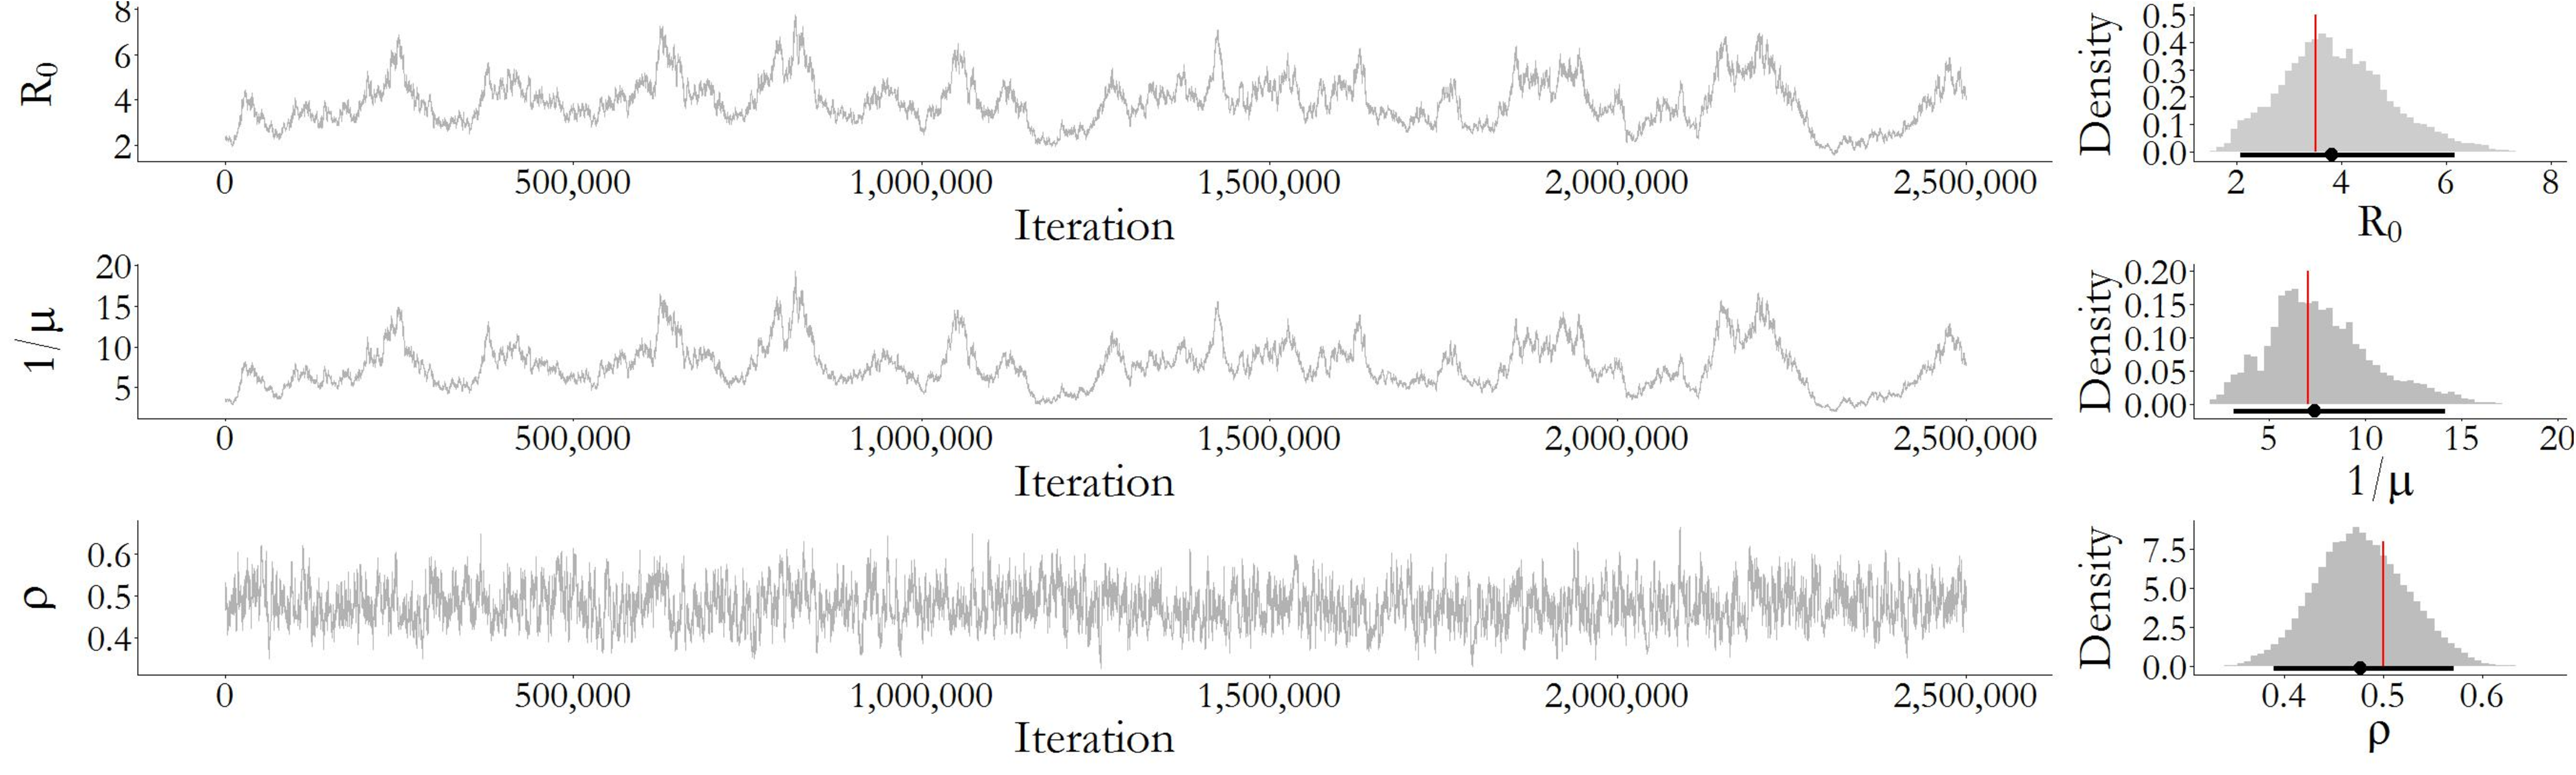
\includegraphics[width=0.9\textwidth]{figures/lna_centered_traces}
\caption[Traceplots for an MCMC chain using a centered LNA parameterization.]{Posterior traceplots for parameters of interest for a single MCMC chain of an SIR model fit to negative binomial distributed incidence data. MCMC targeted the posterior, \ref{eqn:lna_approximate_posterior}, alternately updating the non--restarting LNA for $ \bNtil|\btheta,\bY $ via elliptical slice sampling, and $ \btheta|\bNtil,\bY $ via a multivariate random walk Metropolis algorithm. $ R_0 = \beta N / \mu$ is the basic reproductive number, $ 1/\mu $ is the mean infectious period duration, and $ \rho $ is the mean case detection rate. The true values of $ R_0,\ 1/\mu,$ and $ \rho $ were 3.5, 7, and 0.5, respectively.}
\label{fig:lna_centered_traces}
\end{figure}

\subsubsection{Non--centered Parameterization}
\label{subsubsec:noncentered_parameterization}	

We can improve the mixing of our MCMC chains by reparameterizing the log--incidence process as a deterministic mapping of standard normal random variables, $ \bZ\sim MVN(\bs{0},\mb{I}) $, which are \textit{a priori} independent of the model parameters. Let $ \bNtil(t_\ell)\sim MVN(\bmu(t_\ell),\bSigma(t_\ell) $ and $ \bZ(t_\ell)\sim MVN(\bs{0},\mb{I}) $. Then the NCP is given by $ (\btheta,\bZ) $ and maps onto the CP via \begin{align}
\label{eqn:lna_ncp}
 \bNtil(t_\ell) \overset{\mcL}{=}\widetilde{\bW}(t_\ell),\ \widetilde{\bW}(t_\ell) = \bmu(t_\ell) + \bSigma(t_\ell)^{1/2}\bZ(t_\ell).
\end{align} We now target the joint posterior of the model parameters and the non--centered LNA draws,
\begin{align}
\label{eqn:lna_noncentered_posterior}
\pi(\btheta,\bZ|\bY) &\propto L(\bY|\doLNA(\bZ,\btheta,\mcI))\ind{\bN(\bZ,\btheta,\mcI)\in\mcS_N^R}\ind{\bX(\bZ,\btheta,\mcI)\in\mcS_X^R}\pi(\bZ)\pi(\btheta).
\end{align}
We will denote by $ \bN(\bZ,\btheta,\mcI) $ and $ \bX(\bZ,\btheta,\mcI) $ the incidence and prevalence sample paths that are output by the \doLNA\ procedure. The procedure for this mapping, denoted \doLNA, is presented in Algorithm (\ref{alg:doLNA}). 

\begin{algorithm}
	\caption{Mapping standard normal draws onto LNA sample paths.}
	\label{alg:doLNA}
	\begin{algorithmic}[1]
		\Procedure{doLNA}{$ \bZ,\btheta,\mcI $}
		\State \textbf{initialize: }$ \bX(t_0) \gets \bX_0,\ \bN(t_0) \gets \bs{0},\ \bNtil(t_0) \gets \bs{0},\ \bmu(t_0) \gets \bs{0},\ \bSigma(t_0) \gets \bs{0} $
		\For{$ \ell = 1,\dots,L $}
		\State $ \bmu(t_\ell),\ \bSigma(t_\ell) \gets $ solutions to (\ref{eqn:lna_ode_drift}) and (\ref{eqn:lna_ode_diffusion}) over $ (t_{\ell-1}, t_\ell] $
		\State $ \bNtil(t_\ell)\gets \bmu(t_\ell) + \bSigma(t_\ell)^{1/2}\bZ(t_\ell) $ \Comment{non--centered parameterization}
		\State $ \bN(t_\ell)\gets \bN(t_{\ell-1}) + \exp(\bNtil(t_\ell)) - \bs{1} $
		\State \textbf{restart initial conditions:} 
		\State {\hspace{0.2in} $ \bX(t_\ell) \gets \bX(t_{\ell-1}) + \bA^T(\bN(t_\ell)-\bN(t_{\ell-1})),\ \bNtil(t_\ell) \gets \bs{0},\ \bmu(t_\ell)\gets\bs{0},\ \bSigma(t_\ell)\gets\bs{0} $ }
		\EndFor
		\State \hspace{-0.25in}\Return \Comment{return incidence and/or prevalence sample paths}
		\State$\bN = \left \lbrace\bN(t_0),\bN(t_1),\dots,\bN(t_L)\right \rbrace,\ \bX = \left \lbrace \bX(t_0),\ \bX(t_1),\dots,\bX(t_\ell) \right \rbrace $
		\EndProcedure
	\end{algorithmic}
\end{algorithm}

The NCP of the log--incidence process substantially improves the mixing of MCMC chains that alternate between updates to $ \bZ|\btheta,\bY $ and $ \btheta|\bZ,\bY $. Figure \ref{fig:lna_centered_traces} shows traceplots of model parameters for one of MCMC chains for an SIR model fit to Poisson distributed incidence data using the centered parameterization (CP) of the LNA transition density. MCMC was run for 2.5 million iterations, following a tuning run of equal length, but each chain only manages to yield a effective sample sizes for $ R_0 $ and the infectious period duration in the low double digits. In contrast, the NCP yields effective sample sizes per--chain of between 500--700 for each of the model parameters in only 50,000 iterations, following a short tuning run of equal length. Figure \ref{fig:lna_noncentered_traces} shows the traceplot for one of the MCMC chains, which clearly mixes better. 

\begin{figure}[!ht]
	\centering
	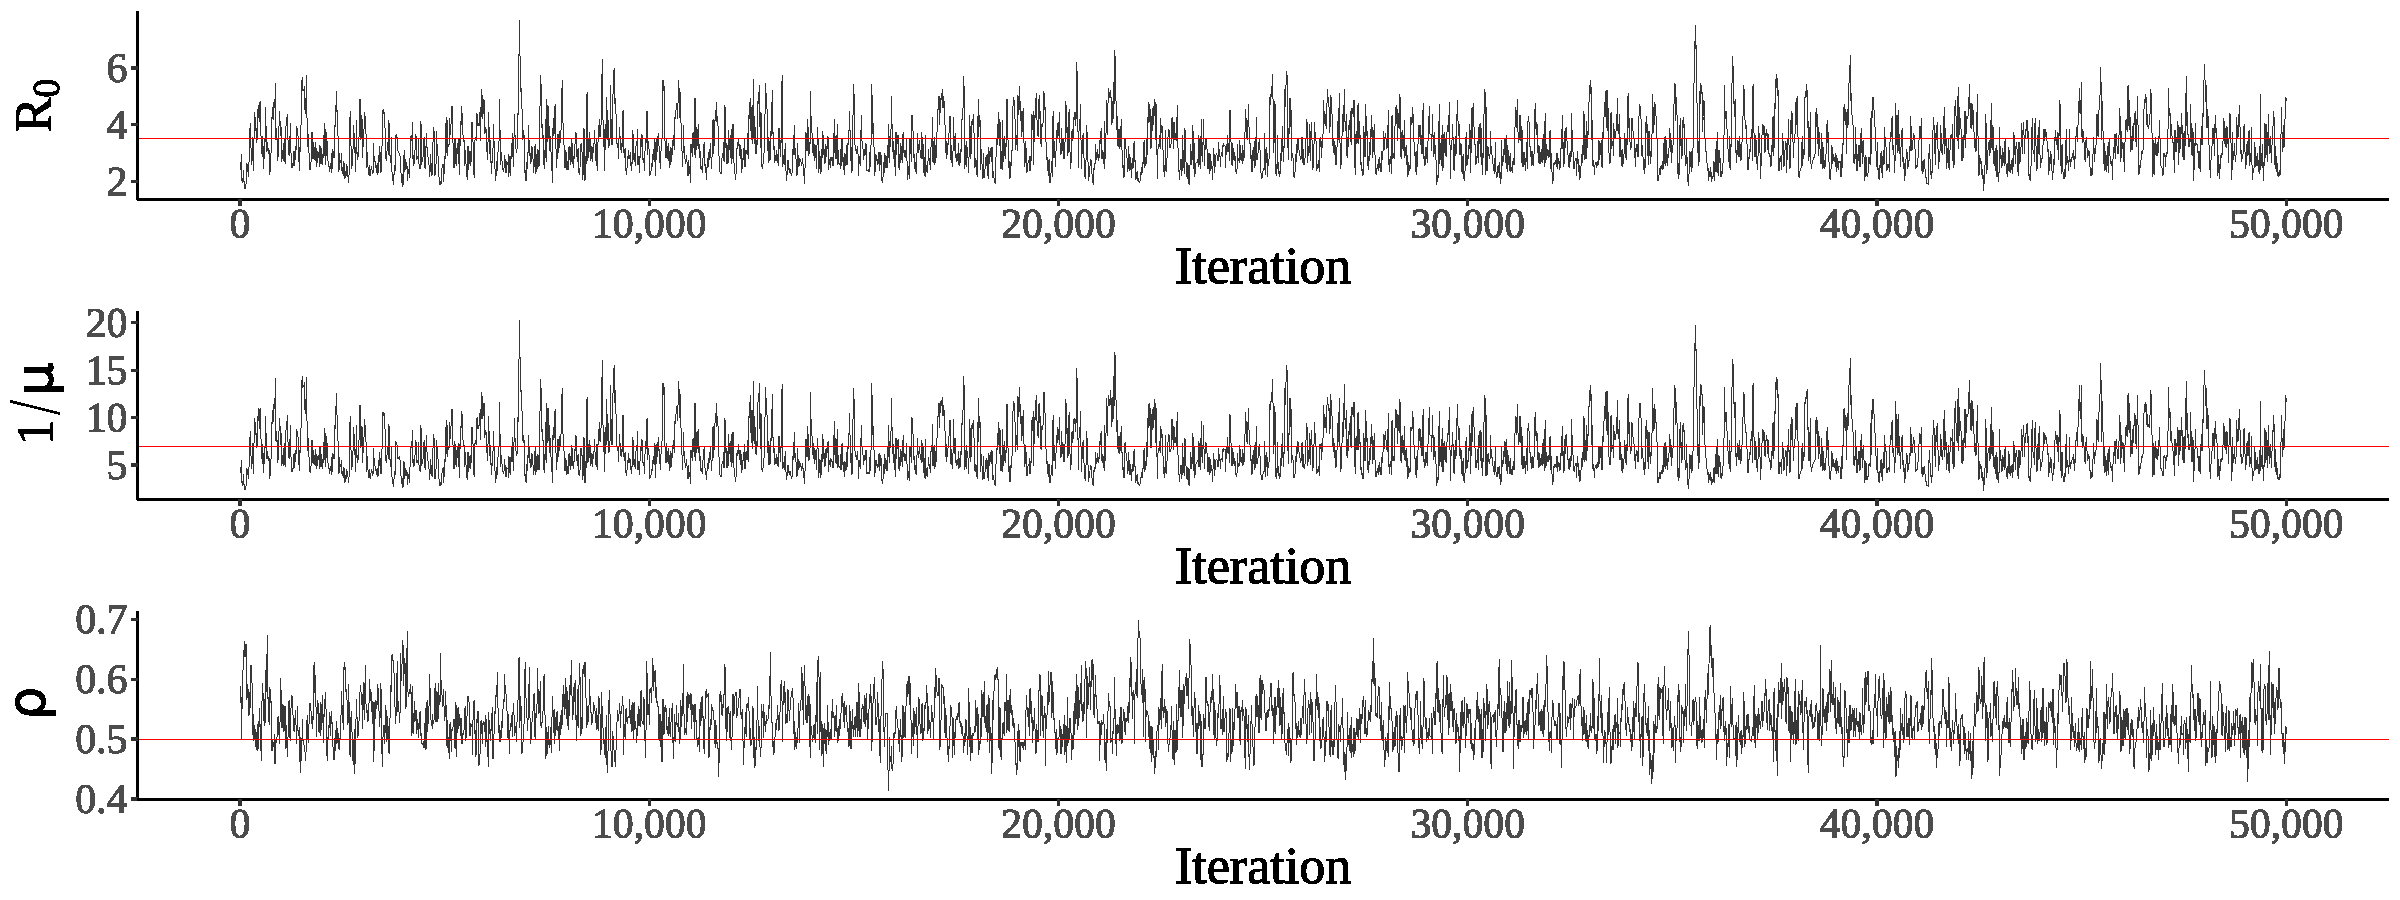
\includegraphics[width=0.9\textwidth]{figures/lna_noncentered_traces}
	\caption[Traceplots for an MCMC chain using a non--centered LNA parameterization.]{Posterior traceplots of parameters of interest sampled by a single MCMC chain of an SIR model fit to Poisson distributed incidence data. MCMC targeted the posterior, \ref{eqn:lna_noncentered_posterior}, alternately updating $ \bZ|\btheta,\bY $ via elliptical slice sampling, and $ \btheta|\bZ,\bY $ via a multivariate random walk Metropolis algorithm. $ R_0 = \beta N / \mu$ is the basic reproductive number, $ 1/\mu $ is the mean infectious period duration, and $ \rho $ is the mean case detection rate. The true values of $ R_0,\ 1/\mu,$ and $ \rho $ were 3.5, 7, and 0.5, respectively.}
	\label{fig:lna_noncentered_traces}
\end{figure}

In each iteration of a DA MCMC algorithm, we alternate between updates to the latent path, conditional on the model parameters, and updates to the parameters, conditional on the latent path. Figure \ref{fig:lna_sampling_diagram}, which depicts the CP and NCP representations of an LNA path, provides some insight into why the NCP improves MCMC mixing. Under the CP (top plot), updates to $ \btheta|\bNtil,\bY $ are made conditionally on a \textit{fixed} LNA path. Therefore, proposed parameter values are accepted depending on whether they are concordant with the data \textit{and} the current path. Even small perturbations to model parameters can result in shifts of the LNA transition densities (grey densities) that would render the current path (red points) unlikely under the proposal. In contrast, perturbations to parameters implicitly perturb the LNA path even as the LNA draws, $ \bZ $, are clamped to their current values. 

\begin{figure}[!ht]
	\centering
	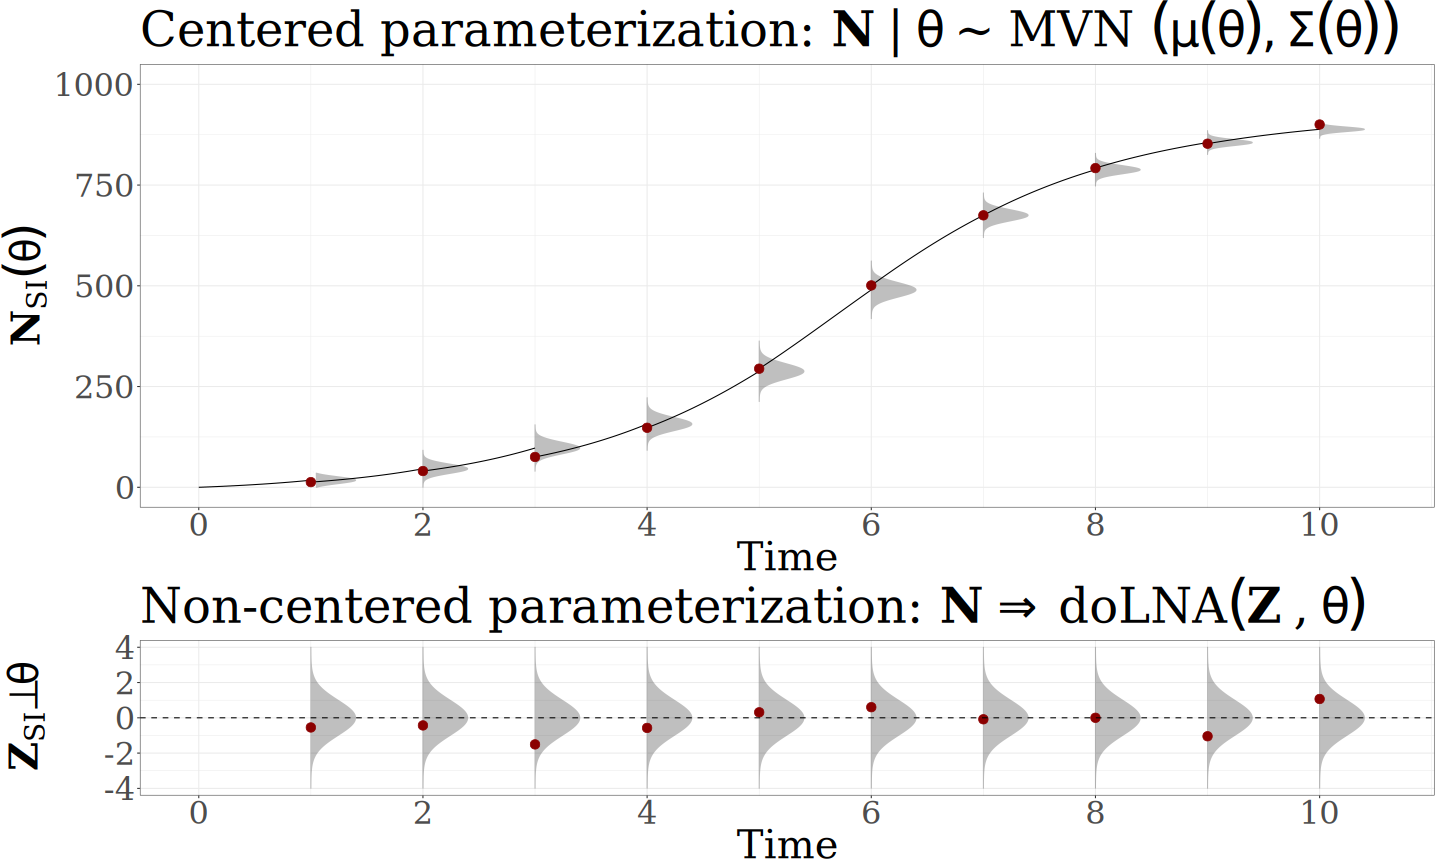
\includegraphics[width=0.9\textwidth]{figures/lna_sampling_diagram}
	\caption[Centered and non--centered LNA paths.]{Centered (top) and non--centered (bottom) parameterizations of an LNA incidence path. In the CP, the log--incidence is normally distributed with mean and covariance obtained by solving the LNA ODEs, (\ref{eqn:lna_ode_drift}) and (\ref{eqn:lna_ode_diffusion}). In the NCP, the log--incidence is a draw from a standard normal distribution that is deterministically mapped to a sample path via the $ \doLNA $ algorithm. In both the CP and NCP, state at the end of each interval determines the initial conditions of the LNA ODEs for the next interval. Plots of CP LNA transition densities are rescaled for clarity.}
	\label{fig:lna_sampling_diagram}
\end{figure}

The NCP of the LNA also plays an important role in facilitating efficient updates of $ \bZ|\btheta,\bY $ via the elliptical slice sampling (ElliptSS) algorithm of \cite{murray2010}, which was detailed in Section \ref{subsubsec:elliptical_slice_sampling} and is presented in Algorithm \ref{alg:elliptss_lna}. ElliptSS is an efficient and easy to implement MCMC algorithm for sampling latent Gaussian random variables, $ \bZ $, in models where the posterior of can be decomposed as the Gaussian prior for $ \bZ $ and an arbitrary likelihood, $ L(\bY|\bZ,\btheta) $, i.e.,
\begin{equation}
\label{eqn:eliptss_posterior_decomp}
\pi(\btheta,\bZ|\bY)\propto L(\bY|\bZ,\btheta)MVN(\bZ;\mu_\bZ,\bSigma_\bZ).
\end{equation}
The target posterior under the LNA NCP, (\ref{eqn:lna_noncentered_posterior}), is of this form, regardless of whether the LNA is restarted at the beginning of each inter--observation interval, as in \cite{fearnhead2014}, or the non--restarting version is used as in \cite{komorowski2009}. Note that the CP cannot be expressed as a jointly Gaussian collection of random variables with complete data likelihood of the form (\ref{eqn:eliptss_posterior_decomp}) when we use the restarting version of the LNA. Although each transition density, (\ref{eqn:lna_transition_density}), is itself Gaussian, the joint LNA path, $ \bN $, is not \textit{a priori} Gaussian when the LNA ODEs are restarted since the mean of $ \bN(t_\ell) $ depends non--linearly on the value of $ \bN(t_{\ell-1}) $. The quality of the LNA approximation is known to degenerate over long time intervals. Restarting the LNA ODEs has been established to improve the approximation when analyzing time series data of non--negligible length \cite{fearnhead2014,giagos2010inference}. Hence, use of the NCP is critical to enabling the use of ElliptSS for jointly updating of $ \bZ|\btheta,\bY $ when using the restarting version of the LNA. 

We note that the elliptical slice sampling Algorithm \ref{alg:elliptss_lna} differs slightly from, but is equivalent to, the algorithm in \cite{murray2010} regarding how the initial proposal is made. The original algorithm was modified so that the distribution of angles for accepted proposals would be symmetric about zero in order to facilitate tuning of the initial bracket width. We have found that shrinking the initial bracket width often improves computational efficiency when fitting more complex models. This is discussed further in Section \ref{sec:lna_init_bracket_width}.

\begin{algorithm}[!ht]
	\caption{Sampling LNA draws via elliptical slice sampling.}
	\label{alg:elliptss_lna}
	\begin{algorithmic}[1]
		\Procedure{\doElliptSS}{$ \bZ_{cur},\btheta,\bY,\mcI,\omega = 2\pi $}
		\State Sample ellipse: $ \bZ_{prop} \sim N(\bs{0}, \mb{I}) $
		\State Sample threshold: $ u|\bx \sim \mr{Unif}(0, L(\bY|\doLNA(\bZ_{cur},\btheta,\mcI))) $
		\State Position the bracket and make initial proposal: \vspace{-0.1in}
		\begin{align*}
		\psi &\sim \mr{Unif}(0,\omega)\\
		L_\psi &\leftarrow -\psi;\ R_\psi \leftarrow L_\psi + \psi\\
		\phi &\sim \mr{Unif}(L_\psi,R_\psi)
		\end{align*}
		\State Set $ \bZ' \leftarrow \bZ_{cur}\cos(\phi) + \bZ_{prop}\sin(\phi) $. 
		\If{$ L(\bY|\doLNA(\bZ',\btheta,\mcI)) > u $}{ accept $ \bZ' $}
		\State\Return{ $ \bZ' $}
		\Else
		\State Shrink bracket and try a new angle:
		\State{\textbf{If:} $ \phi < 0 $}{ \textbf{then: }$ L_\phi \leftarrow\phi $ }{ \textbf{else: }$ R_\phi \leftarrow \phi $}
		\State $ \phi \sim \mr{Unif}(L_\phi, R_\phi) $
		\State \textbf{GoTo:} 5
		\EndIf
		\EndProcedure
	\end{algorithmic}
\end{algorithm}

\subsubsection{Initializing the LNA Draws}
\label{subsubsec:lna_init}
In simple models, reasonable parameter values will generally lead to valid LNA paths for initial $ \bZ\sim MVN(\bs{0},\mb{I}) $, i.e., paths that satisfy the monotonicity and positivity conditions, and thus have non--zero likelihood. However, this is not necessarily the case for complex models with many types of transition events, or when the time--series of incidence counts is long. One option is to include a re--sampling step after line 6 in Algorithm \ref{alg:doLNA}, in which $ \bZ(t_\ell) $ is redrawn in place until the conditions for a valid path over the interval are met. It is important to note that such a procedure does not sample from the correct distribution since $ \bZ $ is not actually a truncated multivariate Gaussian. To correct for this, we will ``warm--up" the LNA path with an initial run of $ \doElliptSS $ iterations in which the likelihood only consists of the indicators for whether the path is valid. Finally, note that ElliptSS, or any valid MCMC algorithm for updating $ \bZ|\btheta,\bY $ for that matter, will never lead to an invalid LNA path being accepted if the current LNA draws and model parameters correspond to a valid path. Similarly, updates to model parameters conditional on the LNA draws will also preserve the validity of LNA paths.

\subsubsection{Parameter Updates}
\label{subsubsec:lna_param_updates}
Each MCMC iteration will consist of a number of ElliptSS updates, typically one but possibly 2--3 for complex models, followed by a set of parameter updates. We will generally use either a global adaptive random walk Metropolis algorithm (Algorithm 4 in \cite{andrieu2008tutorial}) or the adaptive non--isotropic multivariate normal slice sampler (MVNSS) presented in Section \ref{subsubsec:slice_sampling}. In models where the initial state, $ \bX_0 $, is not fixed, we will assign a strongly informative prior $ \bX_0 \sim TMVN_{\mcS_X^R}\left (N\mb{p}, N(\diag(\mb{p}) - \mb{p}\mb{p}^T)\right ) $, which is a truncated multivariate normal approximation to a multinomial with initial state probabilities, $ \mb{p} $, constrained to the state space of compartment volumes. We update $ \bX_0 $ jointly with the LNA path via ElliptSS. Additional details are presented in Section \ref{sec:lna_init_volumes}.

We have found it helpful, for the purpose of assigning sensible priors to model parameters and for improving MCMC mixing and convergence, to parameterize the estimation scale on which the MCMC explores the parameter space in terms of how the parameters directly affect the model dynamics. For the SIR model, this might mean re-expressing the model parameters in terms of the basic reproductive number of an outbreak, $ R0 = \beta N /\mu $, and the recovery rate, $ \mu $. Additionally, we would like our estimation scale to be unconstrained and therefore sample (and either accept or reject) values for $ \log(R0) $ and $ \log(\mu) $. The importance of appropriately parameterizing the estimation scale is discussed at length in Section \ref{sec:est_scale_discussion}. 

\subsection{Implementation}
\label{subsec:lna_implementation}
The algorithms for approximate inference via the LNA and ODE models are implemented in the \texttt{stemr} $ \R $ package, which can be available, along with vignettes for reproducing our results, from the following stable GitHub repository: \texttt{https://github.com/fintzij/stemr}. The implementation is flexible and provides facilities for specification of arbitrary SEM dynamics, a variety of emission probability distributions, and capabilities for accommodating time--varying covariates, time--varying parameters, and deterministic forcings. Computationally intensive operations are implemented in \texttt{C++} via \texttt{Rcpp} and \texttt{RcppArmadillo} \cite{rcpp,rcpparmadillo}. ODE integration functions are dynamically compiled in \texttt{C++} with the help of the \texttt{odeintr} R package \cite{odeintr} and ODEs can be integrated using a variety of methods available in the \texttt{Odeint C++} library \cite{ahnert2011odeint}. Additional aspects of the implementation are discussed in Section \ref{sec:lna_implementation_vignettes}.

\section{Simulations}
\label{sec:lna_simulations}

\subsection{Motivating Use of the LNA --- Comparison with Common SEM Approximations}
\label{subsec:lna_coverage}

The LNA is by no means the only approximation of the transition density of the MJP representation of a SEM. In the following subsection, we will illustrate why the LNA is an attractive choice, balancing computational cost with fidelity of the MJP approximation. We benchmark the LNA against two commonly used approximations of the MJP: the deterministic approximation given by a system of deterministic ODEs that are the functional infinite population limit of the MJP \cite{fuchs2013inference}, and a discrete--time approximation of the MJP using a multinomial modification of the $ \tau $--leaping algorithm (MMTL) \cite{breto2011compound} to simulate epidemic paths within a particle marginal Metropolis--Hastings (PMMH) framework \cite{andrieu2010particle}. The ODE approximation was chosen because of its ubiquity in the study of epidemic modeling, while the MMTL approximation in combination with PMMH was chosen because of a straightforward and general implementation in the popular \texttt{pomp} package in \texttt{R} \cite{pompjss}. Arguably, the MMTL approximation is somewhat closer to the original MJP than the LNA since it preserves the discreteness of the latent state space, while the ODE approximation, being deterministic, is further removed from the MJP.

The fidelity of each approximation to the original MJP depends on the population size and the epidemic dynamics. In relative terms, outbreaks with explosive dynamics in large populations will tend to deviate less from their infinite population deterministic limits than outbreaks that occur in small populations, that are less contagious, or that are characterized by uncertainty in the probability and timing of a major outbreak. We fit SIR models to 500 datasets simulated under a range of SIR dynamics. Each dataset is simulated by drawing the model parameters from a set of prior distributions, simulating an outbreak via Gillespie's direct algorithm \cite{gillespie1976general}, and finally simulating the dataset as a negative binomial sample of the true incidence. Datasets arising from outbreaks that died off immediately were discarded and re--simulated, while datasets arising from outbreaks lasting longer than 50 epochs were truncated at 50 observations. SIR models were then fit via the LNA, ODE, and MMTL approximations under the priors from which the parameters were drawn. The simulation was repeated under three different regimes for the population size and the initial number of infected individuals, reflecting different levels of initial stochasticity in the epidemic trajectory. The priors and population sizes (Table \ref{tab:lna_coverage_sim}) were chosen because they were typical of settings in which the methods might reasonably be applied, e.g., the population sizes are not so big that the outbreaks would evolve deterministically, nor so small that the approximations would be unreasonable. All individuals who were not initially infected were susceptible at the start of each outbreak (i.e., no individuals with pre-existing immunity).  The population sizes and initial conditions were fixed at their true values. Hence, the only model misspecification was in the approximation used for the latent epidemic process. Additional results and details about the simulation setup are provided in Section \ref{sec:lna_coverage_supplement}. We also performed four analogous supplementary simulations, with similar results, where we generated datasets under fixed parameter regimes (presented in Section \ref{sec:lna_fixedpar_coverage}).

\begin{table}[!ht]
	\caption[LNA coverage simulation settings.]{Population sizes, initial conditions, and priors under which datasets were simulated. Five hundred datasets were simulated for each of the population size regimesEach outbreak was simulated from a MJP with SIR dynamics. The observed incidence was a negative binomial sample of the true incidence in each inter--observation interval.}
	\label{tab:lna_coverage_sim}
	\small
	\centering
	\begin{tabular}{lccc}
		\hline
		& \textbf{Regime 1} & \textbf{Regime 2} & \textbf{Regime 3} \\\hline
		\textbf{Population size ($ N $)} & 10,000 & 50,000 & 250,000 \\ 
		\textbf{Initial infecteds ($ I_0 $)} & 1 & 5 & 25 \\
		\hline
		&&&
	\end{tabular} 

	\begin{tabular}{cllc}
		\hline
		\textbf{Parameter} & \textbf{Interpretation} & \textbf{Prior} & \textbf{Median (95\% Interval)} \\ \hline
		$ R0-1 $ & Basic reproduction \# - 1 & LogNormal(0, 0.25) & $ \implies R0 = $ 2.00 (1.38, 3.66) \\ 
		$ 1/\mu $ & Mean infectious period & LogNormal(-0.7, 0.35)& 1.43 (0.72, 2.84) \\
		$ \rho / (1-\rho) $ & Odds of case detection & LogNormal(0, 1) & $ \implies \rho =$ 0.5 (0.12, 0.88) \\
		$ \phi $ & Neg.Binom. overdispersion & Exponential(0.1) & 6.93 (0.25, 36.89)\\
		\hline
	\end{tabular}
\end{table}

\subsubsection{Results}

This simulation was designed to be generous to the approximations that were used in fitting SEMs to the simulated data. The initial compartment counts and true population sizes were known, and there was no misspecification with respect to either the sampling model or the epidemic dynamics. Despite this, the ODE models struggle to reliably recover the true parameters, particularly those governing the sampling process. As shown in Figure \ref{fig:lna_coverage_main}, coverage of credible intervals for ODE models was low for all model parameters, and this was only somewhat mitigated as the population size increased. Coverage of credible intervals for models fit via the LNA and via MMTL was close to the nominal 95\% level for all model parameters in all three population size regimes. Further inspection of the posterior median errors (middle row of Figure \ref{fig:lna_coverage_main}) and the widths of 95\% credible intervals (bottom row of Figure \ref{fig:lna_coverage_main}) provides intuition for why the ODE performs so poorly. Estimates of the case detection probability tend to be high and estimates of the negative binomial over--dispersion parameter are low (corresponding to large variances in the conditional distribution of observed incidence). Furthermore, credible intervals for the basic reproductive number and recovery rate obtained via the ODE approximation tend to be narrower than LNA and MMTL credible intervals. This is in agreement with findings by other authors who have found that ODE models tend to underestimate uncertainty in epidemic dynamics (see e.g., \cite{king2015avoidable}). Taken together, these results suggest that the LNA is, at least in this simple example, about as good at approximating the original MJP as is the more exact MMTL. 

\begin{figure}[p]
	\begin{fullpage}
		\centering
		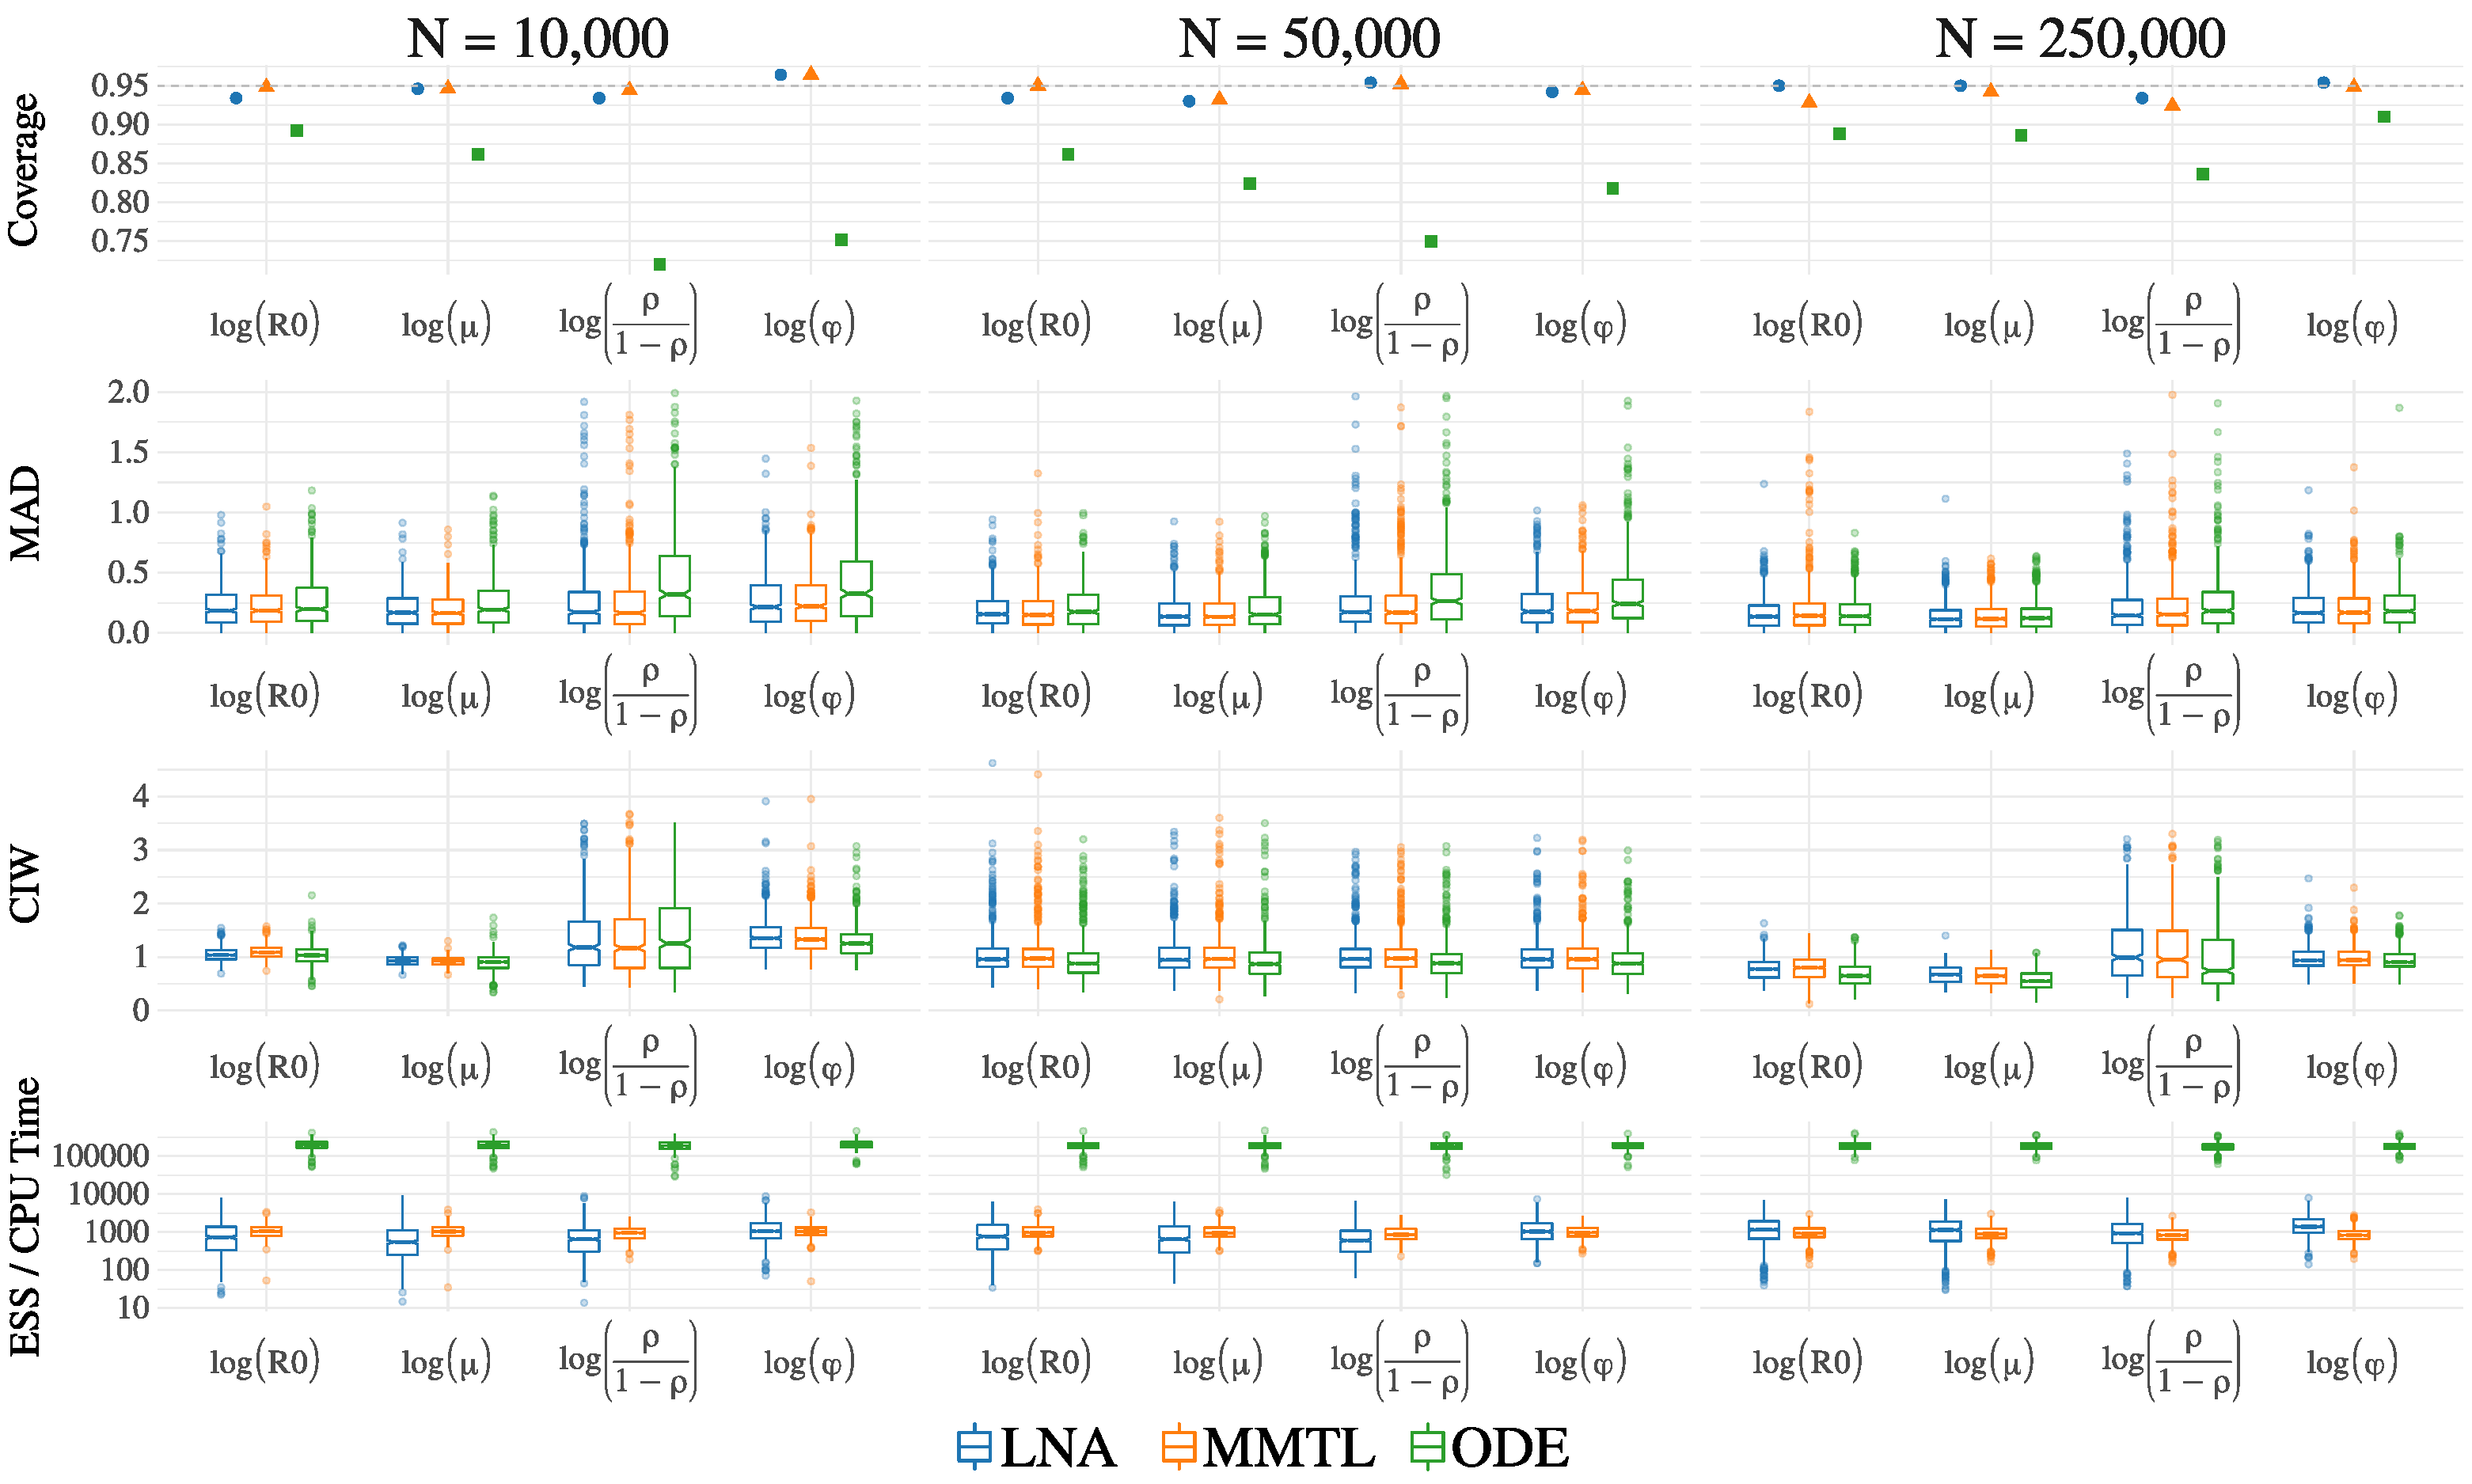
\includegraphics[width=0.95\textwidth]{figures/lna_coverage_plots_main}
		\caption[Coverage simulation results for SIR models fit via the LNA, ODE, and MMTL approximations.]{Comparison of SIR models fit to 500 datasets simulated in populations of three different sizes. Models were fit via the linear noise approximation (LNA), multinomial modified $ \tau $--leaping (MMTL) within particle marginal Metropolis--Hastings, and deterministic ordinary differential equations (ODE). $ R_0 $ is the basic reproductive number of an outbreak, $ \mu $ is the recovery rate, $ \rho $ is the negative binomial case detection probability, $ \phi $ is the negative binomial over--dispersion parameter. The rows correspond to the proportion of runs where the 95\% Bayesian credible interval covered the true parameter values, the posterior median deviation, and the widths of 95\% Bayesian credible intervals. The simulation was repeated for three regimes of population sizes and initially infected individuals (columns).}
		\label{fig:lna_coverage_main}
	\end{fullpage}
\end{figure}

We note that these results are not intended to suggest that there is no place for ODE models in the computational toolbox of disease modelers. To the contrary, when time is of the essence, as in an outbreak setting, crude estimates via the ODE may be obtained quickly. Average ODE run times were substantially shorter than LNA and MMTL run times and required far less CPU time per effective sample (see Table \ref{tab:lna_coverage_compstats}). ODE models are also appealing because they lend themselves to analytic characterizations of various aspects of the outbreak dynamics, e.g., relating the final outbreak size to the basic reproductive number (see, e.g., \cite{andersson2000stochastic,britton2018,keeling2008}).

 In this simple simulation, the LNA and MMTL approximations had comparable computational performance, with the LNA perhaps being somewhat faster, but also with the caveat that comparing the ODE/LNA approximations with the MMTL approximation on the basis of computational performance is a bit misleading since the comparison would have turned out differently had we made other choices for the LNA and MCMC settings (e.g., timestep of MMTL, number of particles in PMMH, or tuning the initial EllipSS bracket width for the LNA). The important point to make regarding computational performance is that as model dynamics get more complex and the time series get longer, approximations, such as MMTL, that are used within a particle filter framework, such as PMMH, will become computationally infeasible. In many cases, the lack of an adequate model from which to simulate particle paths will lead to issues of particle degeneracy and an inability to fit even simple models (see \cite{fintzi2017efficient} for an example). Indeed, PMMH was abandoned as a computational strategy for analyzing Ebola data in later sections because of difficulty fitting SEMs with reasonable effort. However, as we shall see in the following sections, the LNA remains performant even as the model dynamics increase in complexity. 
 
 \begin{table}[!h]
 	\caption[Computational performance of the ODE, LNA, and MMTL approximations.]{Run times, effective sample sizes, and relative geometric mean (GM) log--posterior effective sample size (ESS) per CPU time for models fit via the ODE, LNA, and MMTL approximations. Run times and ESS are computed over all chains. The GM log--posterior ESS/CPU time was computed over the five chains for each model and divided by the corresponding GM ESS/CPU time for the MMTL model. We report 50\% (2.5\%, 97.5\%) quantiles of the CPU time, ESS, and relative GM ESS/CPU time.}
 	\label{tab:lna_coverage_compstats}
 	\footnotesize
 	\centering
 	\begin{tabular}{lccc}	
 		\hline	
 		& \textbf{ODE} & \textbf{LNA} & \textbf{MMTL} \\\hline
 		\textbf{CPU time (minutes)} &  0.42 (0.23, 0.64) & 27.78  (12.03, 56.25) & 86.96 (40.47, 159.68) \\ 
 		\textbf{Effective sample size} & 5745 (4557, 6616) & 4067   (346, 11313) & 6834 (3764, 11879) \\
 		\textbf{GM ESS/CPU time vs. MMTL} & 180 (90, 350) & 1.87 (0.14, 8.84) & --- \\
 		\hline
 		&&&
 	\end{tabular} 
 \end{table}


\subsection{Assessing Model Fit}
\label{subsec:lna_model_diags}

Although model assessment is not the focus of this work, we emphasize the importance of diagnostics and briefly present several tools that can be used to interrogate SEMs fit via the LNA. We highlight the following diagnostics because they are easily implemented post-hoc and require little additional effort beyond caching random quantities throughout the MCMC run. 

One of the central objectives in infectious disease modeling is to estimate the severity and duration of an outbreak \cite{lofgren2014opinion}. However, the discrete and partial nature of the data makes it difficult to ascertain whether our estimates of the latent epidemic process reconstruct the true path of the outbreak (left plot, Figure \ref{fig:sirdiagplots}). A standard alternative is to check whether the observed incidence is captured in the posterior predictive distribution. 

The partial posterior predictive distribution, shown in the middle plot of Figure \ref{fig:sirdiagplots}, is the predicted observed incidence, conditional on the outbreak being distributed according to the epidemic paths that we believe to be likely given the data at hand (i.e. the latent posterior). Here, new data are sampled using the posterior distribution of the observation model conditionally on the paths in the latent posterior sample. Hence, for replication $ j $, we simulate \begin{equation}
\label{eqn:lna_partial_postpred}
Y_\ell^{(j)}|\bN_{post}^{(j)},\btheta_{post}^{(j)} \sim \mr{Neg.Binom.}\left (\mu = \rho^{(j)}\left (N_{SI}^{(j)}(t_\ell) - N_{SI}^{(j)}(t_{\ell-1})\right ),\sigma^2 = \mu + \mu^2 / \phi^{(j)} \right ),
\end{equation} 
where $ \bN_{post}^{(j)} $ and $ \btheta_{post} $ are the $ j^{th} $ posterior samples for the latent path and model parameters. 

The full posterior predictive distribution, shown in the right plot of Figure \ref{fig:sirdiagplots}, is the predicted observed incidence, integrated over the predicted latent incidence given the current data. Under the full posterior predictive distribution, new data are sampled by simulating a new latent path under the posterior distribution of the epidemic model parameters, and then simulating a new dataset conditionally on the simulated path. So, for replication $ j $, we simulate \begin{align}
\label{eqn:lna_full_postpred}
\bZ^{(j)}_{rep} &\overset{i.i.d.}{\sim} N(0,1),\ \bN^{(j)}_{rep} = \doLNA(\bZ^{(j)}_{rep},\btheta_{post}^{(j)},\mcI), \\ 
Y_\ell^{(j)}|\bN_{rep}^{(j)},\btheta_{post}^{(j)} &\sim \mr{Neg.Binom.}\left (\mu = \rho^{(j)}\left (N_{SI}^{(j)}(t_\ell) - N_{SI}^{(j)}(t_{\ell-1})\right ),\sigma^2 = \mu + \mu^2 / \phi^{(j)} \right ),
\end{align} 
where $ \bZ_{rep}^{(j)} $ is a new vector of LNA draws. 

The full posterior predictive distribution provides a diagnostic for whether the joint model for the latent epidemic process and the observation process is reasonable as a data generating mechanism. In contrast, the partial posterior predictive distribution is useful for qualitatively assessing the adequacy of the emission distribution. Note that, when simulating from the full posterior predictive distribution, the replicated paths must still satisfy the constraints on the state space of $ \bN $ and $ \bX $. We can sample from the approximate posterior predictive distribution using the procedure described in Section \ref{subsubsec:lna_init} to avoid rejection sampling. 
\begin{figure}
	\centering
	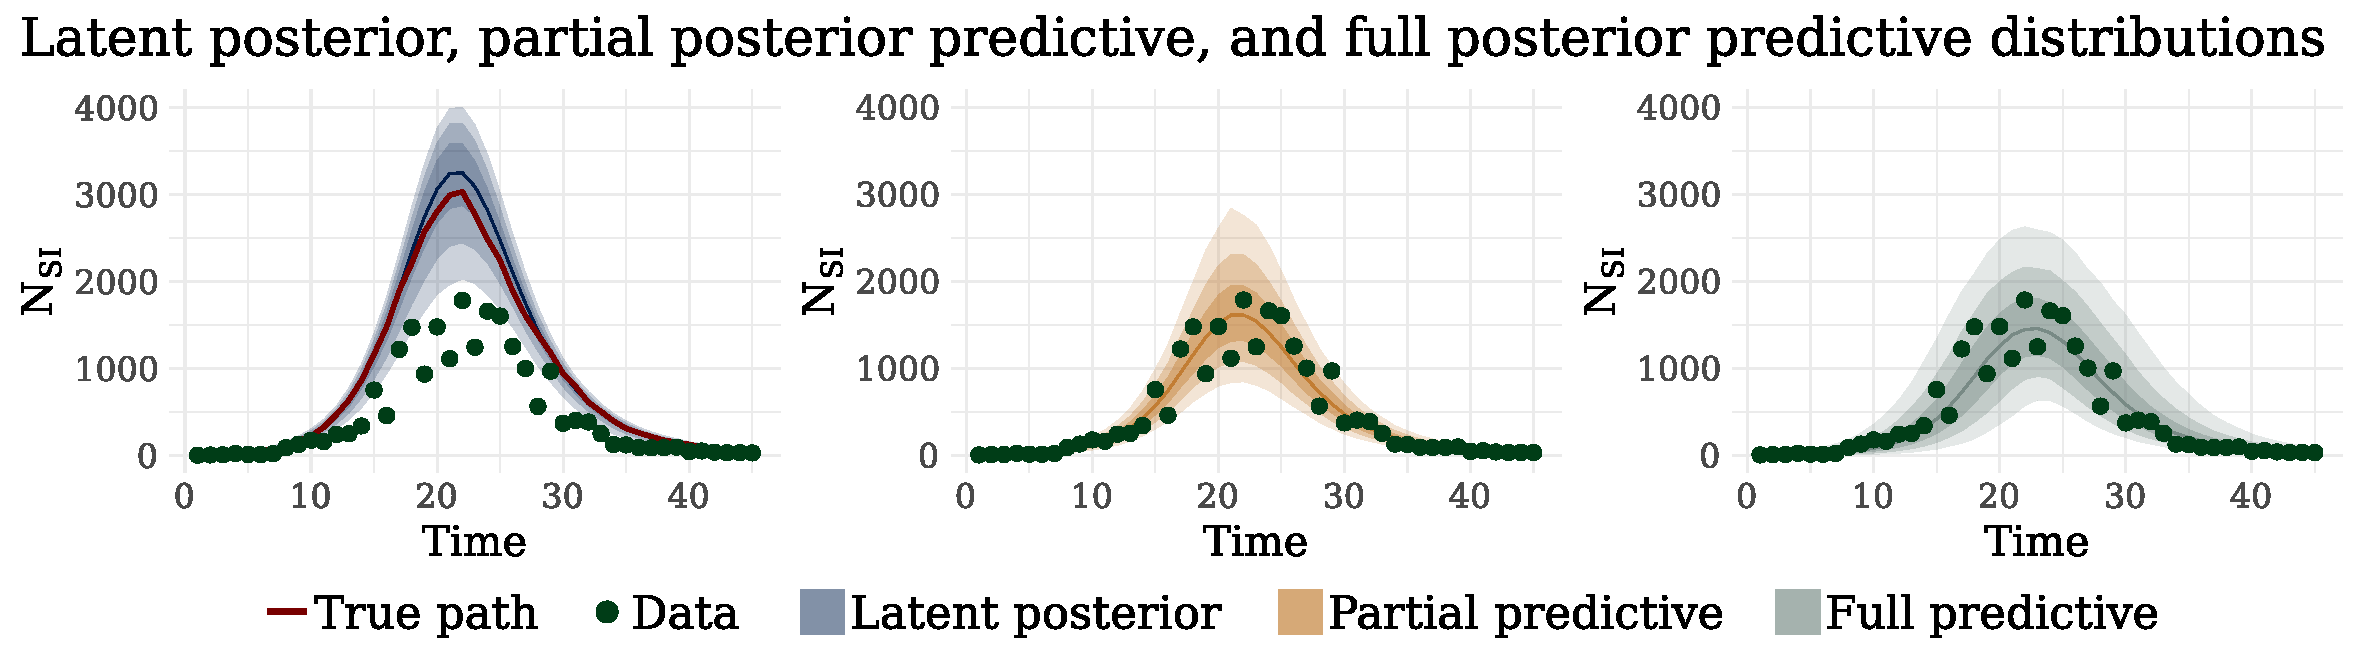
\includegraphics[width=\linewidth]{figures/sir_diag_plots}
	\caption[SIR model latent posterior, partial posterior predictive, and full posterior distributions.]{Estimated latent posterior (left), partial posterior predictive (middle), and full posterior predictive (right) distributions. The true path is the red line in the leftmost plot and the observed incidence counts are the solid green dots. The shaded bands, in order of lightest to darkest, correspond to pointwise posterior 95\%, 80\%, and 50\% credible intervals, with the pointwise posterior median given by the corresponding colored solid line.}
	\label{fig:sirdiagplots}
\end{figure}

The second diagnostic, motivated by ideas presented in \cite{lau2014new}, leverages the structure of LNA draws as i.i.d. standard normal variates to identify time intervals over which the observed incidence suggests that dynamics of the latent process are not well approximated by the LNA prior. The normal CDF values of the LNA draws, $ \bU_\bZ \equiv \Phi(\bZ) \overset{i.i.d.}{\sim} \mr{Unif}(0,1) $, can be understood as latent recursive residuals in the sense of \cite{cox1968general} since each LNA increment is a deterministic function of the model parameters and the LNA draws, $ \bZ $. Suppose that the emission distribution reasonably describes the sampling mechanism by which we the observed incidence is related to the true incidence. Then, the latent residuals for intervals where the latent process is well approximated by the LNA will be approximately uniformly distributed, whereas we would expect to see systematic deviations from uniformity when the LNA is a poor approximation. This is clearly the case in Figure \ref{fig:sirresidplots}, where quantiles of the latent residuals are clearly not uniform towards the start and end of the outbreak. This is not unexpected since the number of MJP transitions during these time periods are relatively low. The interpretation of this diagnostic as an indicator for misspecification in the latent epidemic process depends on the sampling model being approximately correct, and it is thus most useful in conjunction with other model diagnostics. Still, even when the emission distribution is unreasonable, e.g., if the case detection probability varies over time, we might be able to use the latent residuals to identify time intervals where the joint model is misspecified.

\begin{figure}
	\centering
	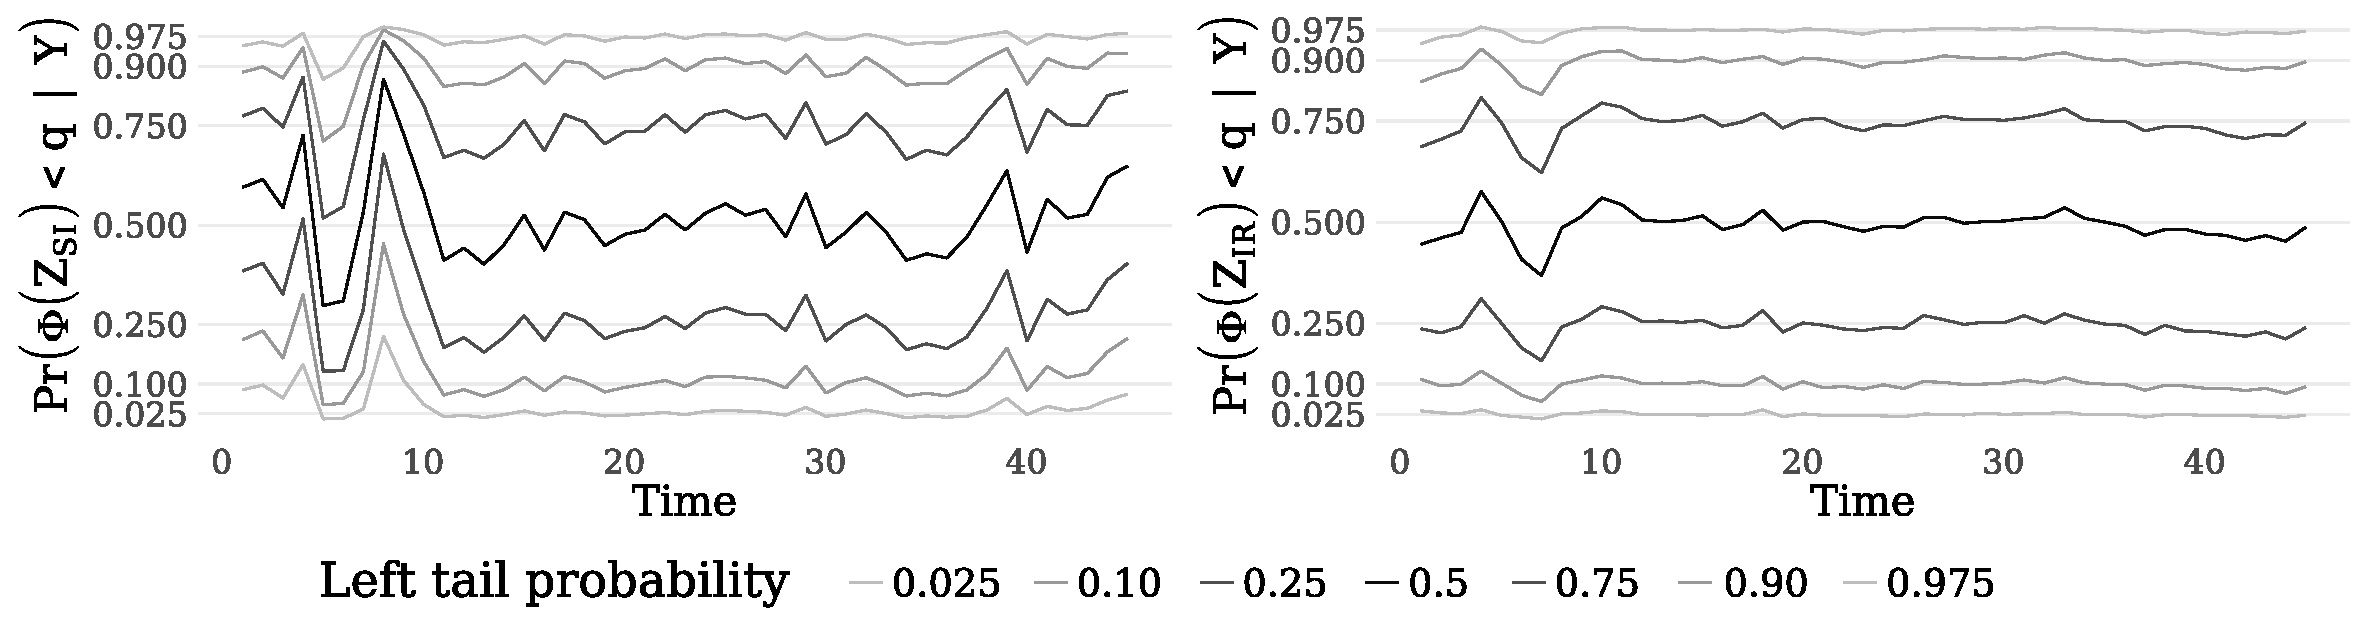
\includegraphics[width=\linewidth]{figures/sir_residplots}
	\caption[SIR model latent recursive residuals.]{Posterior quantiles of latent recursive residuals for infections (left) and recoveries (right). Solid lines of varying shades correspond to the posterior quantiles, light horizontal lines in the background correspond to the theoretical quantiles under the prior.}
	\label{fig:sirresidplots}
\end{figure}

Finally, we can interrogate the validity of the SEM and whether it reflects the temporal dependencies in the data by computing summary statistics for the observed incidence and posterior predictive incidence. A variety of summary statistics are presented in the supplement of \cite{king2015avoidable}, which are computed and compared for the observed and predicted data. These include the lag 1 autocorrelation (ACF) and the detrended autocorrelations at lags 1, 2, and 3. We will also consider the partial autocorrelation function (PACF) \cite{brockwell2013time} of the log--transformed data. We compute the PACF of $ \bYtil = \log(\bY + 0.5) $ at lag $ k $ as 
\begin{align}
\label{eqn:lna_pacf}
\alpha(1)& =  \Cor\left (\bYtil_{(t)}, \bYtil_{(t+1)}\right ), \\
\alpha(k) &= \Cor\left (\bYtil_{(t+k)} - \Proj_{(t,k)}\left (\bYtil_{(t+k)}\right ),\ \bYtil_{(t)} - \Proj_{(t,k)}\left (\bYtil_{(t)}\right )\right ),
\end{align}
where the constant 0.5 is added to stabilize the logarithm for zero counts and $ \Proj_{(t,k)}(\bYtil_{(j)}) $ is the projection of $ \bYtil_{(j)} $ onto the span of $ \bYtil_{(t+1)},\dots,\bY_{(t+k-1)} $ (N.B. this is equivalent to regressing $ \bYtil_{(j)} $ on $ \bYtil_{(t+1)},\dots,\bY_{(t+k-1)} $). The PACF is a measure of the residual autocorrelation at a particular lag, adjusting for the linear dependencies on the intermediate variables. We should expect the PACF of the predicted data in the full posterior predictive distribution to be distributed around zero for lags greater than one since the SEM is a first order Markov process. If the distributions of PACFs for predicted datasets in the partial predictive distribution are pulled away from zero for higher order lags, this may be indicative of long range correlation in the latent process that is unaccounted for by the SEM dynamics. Furthermore, we can compare the PACF for the observed and predicted data to see whether the model reflects the observed temporal dependence. Plots of the observed and predicted PACFs in Figure \ref{fig:sirpacfplots} do not suggest any model misspecification (as expected, since there was none). 

\begin{figure}[!ht]
	\centering
	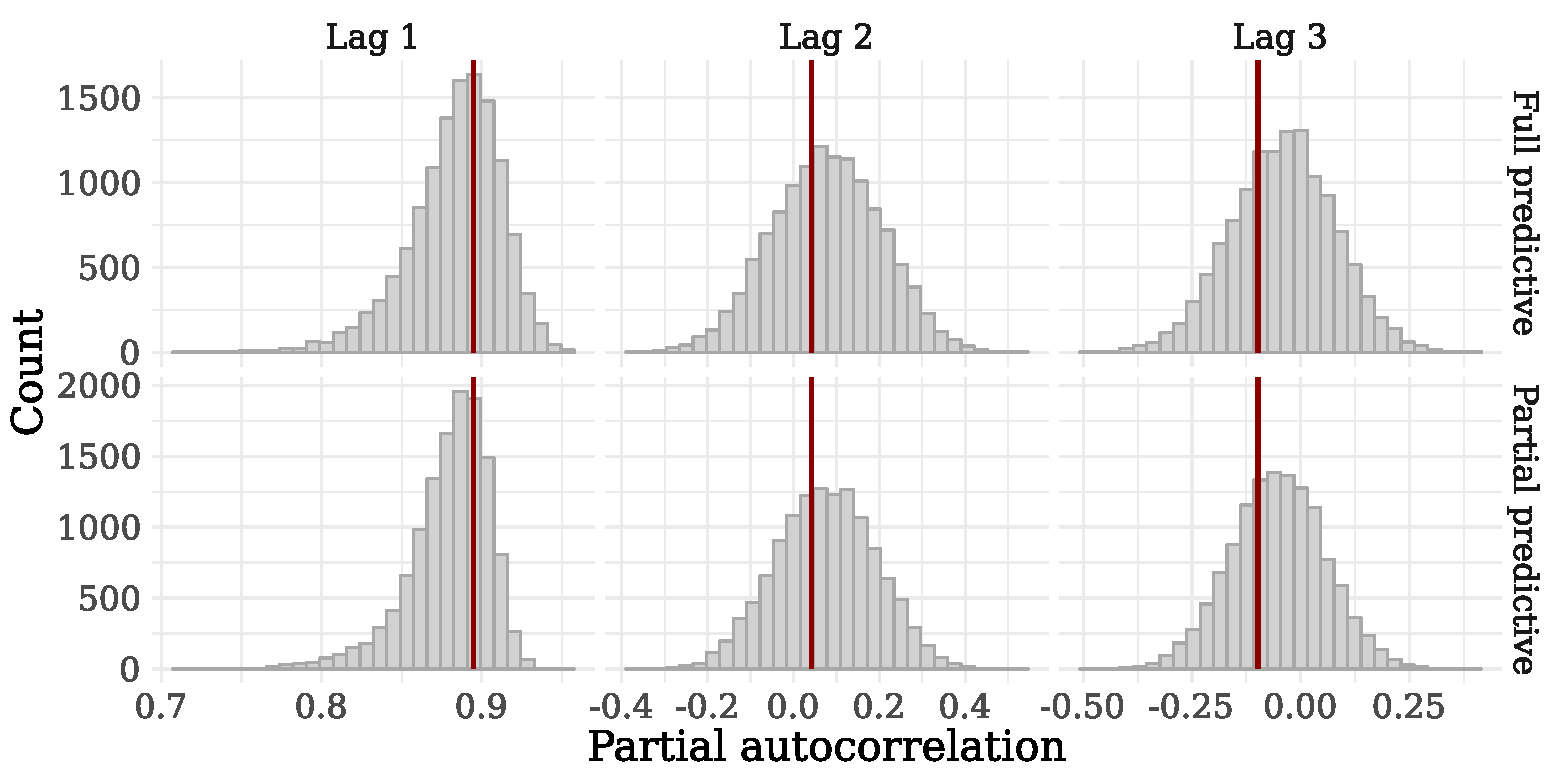
\includegraphics[width=0.9\linewidth]{figures/sir_pacf_plots}
	\caption[Posterior predictive distributions of partial autocorrelations at various lags.]{Distributions of partial autocorrelations at lags 1, 2, and 3 for datasets generated under the full and partial posterior predictive distributions. Vertical red lines are the partial autocorrelations for the observed incidence data at the respective lags.}
	\label{fig:sirpacfplots}
\end{figure}

\subsection{A Stratified SEIR Model for a Simulated Outbreak}
\label{subsec:ebola_synth}

In the next section, we will jointly model the spread of Ebola in Guinea, Liberia, and Sierra Leone during the 2014--2015 outbreak. To do so, we will fit a stratified SEIR model that allows for country specific epidemic dynamics, and transmission between the countries. It should go without saying that this model (or any model), despite being fully stochastic in all aspects of the measurement and epidemic process, is still an overly simplistic abstraction of the outbreak with respect to some obvious and potentially important complexities, e.g., spatial heterogeneity and time varying dynamics. However, it is a good starting point and is non--trivial to fit due to the number of parameters and size of the latent space. Due to the myriad challenges involved in fitting the model, we will first assess its performance in recovering the true parameters and latent path for a simulated outbreak.

We simulated data from a three country SEIR model, diagrammed in Figure \ref{fig:stratified_seir_full_diag}, and described briefly below, with additional details in Section \ref{subsec:ebola_synth_setup}. The simulation was designed to crudely reflect the Ebola outbreak in West Africa and allowed for cross--border transmission via the migration of infected individuals between countries. The three countries differed in their true and effective population sizes, times at which transmission commenced, epidemic dynamics, and case detection probabilities. We included a single changepoint for the basic reproductive number for Guinea at 33 weeks since the outbreak was ongoing longest in that country. The change in transmission dynamics coincided roughly with the WHO declaration of a state of emergency in early August 2014 and the closures of country borders with Liberia and Sierra Leone \cite{coltart2017ebola}. The outbreak was simulated from a MJP via Gillespie's direct algorithm \cite{gillespie1976general} using the parameters in Table \ref{tab:ebola_synth_pars} and the rates in Table \ref{tab:ebola_synth_rates_full}. The observed incidence was a negative binomial sample of the true incidence with the case detection probability varying across countries, but with the same value of over--dispersion.

We fit a stratified SEIR model to the simulated data that was largely the same as the model used in simulating the data, except with respect to migration of infected individuals from one country to another. In this example, as we would expect for the real--world Ebola outbreak, transmission was largely driven by contacts with natively infected individuals. We approximate the contribution of cross--border transmission to the local force of infection by replacing migrations of infected individuals with virtual migrations that modify the effective number of infected individuals in a country. Hence, we replace the rates at which individuals become infected in country A and import infections from countries B and C,
\begin{align}
\label{eqn:foi_migration}
\lambda_{SI}^A &= \beta_A S_A I_A, \\
\lambda_I^{BA} &= \alpha_BI_B,\ \hspace{0.1in} \lambda_I^{CA} = \alpha_CI_C,
\end{align}
with the approximate rates,
\begin{align}
\label{eqn:foi_virtual}
\lambda_{SI}^A &= \beta_AS_A(I_A + \alpha_{BA}I_B + \alpha_{CA}I_C)\\
\lambda_I^{BA} &= \lambda_I^{CA} = 0,
\end{align}
where $ \beta_A $ is the per--contact rate of infection in country A, and the $ \alpha $ parameters are the rates of real or virtual migration of infected individuals from countries B and C. We note that the models are approximately equivalent to the extent that the infectious period durations in each country are similar and that the contribution to the local force of infection from other countries is relatively minimal. The upside is that the quantities, $ \alpha_{BA}I_B $ and $ \alpha_{CA}I_C$, are interpretable as the effective number of infected individuals from countries B and C with whom susceptibles in country A come into contact. The approximate model is also more computationally since we have fewer ODEs to solve in the LNA approximation, and fewer boundary conditions on the LNA state space to meet. Finally, the approximate model is arguably more appropriate since the LNA approximation for infectious migration events is dubious due to low migration rates. The full model with migration was fit as a supplementary analysis and yielded equivalent results (see Section \ref{subsec:ebola_synth_fullmod_res}).  

\begin{figure}[!ht]
	\resizebox {\linewidth} {!} {
		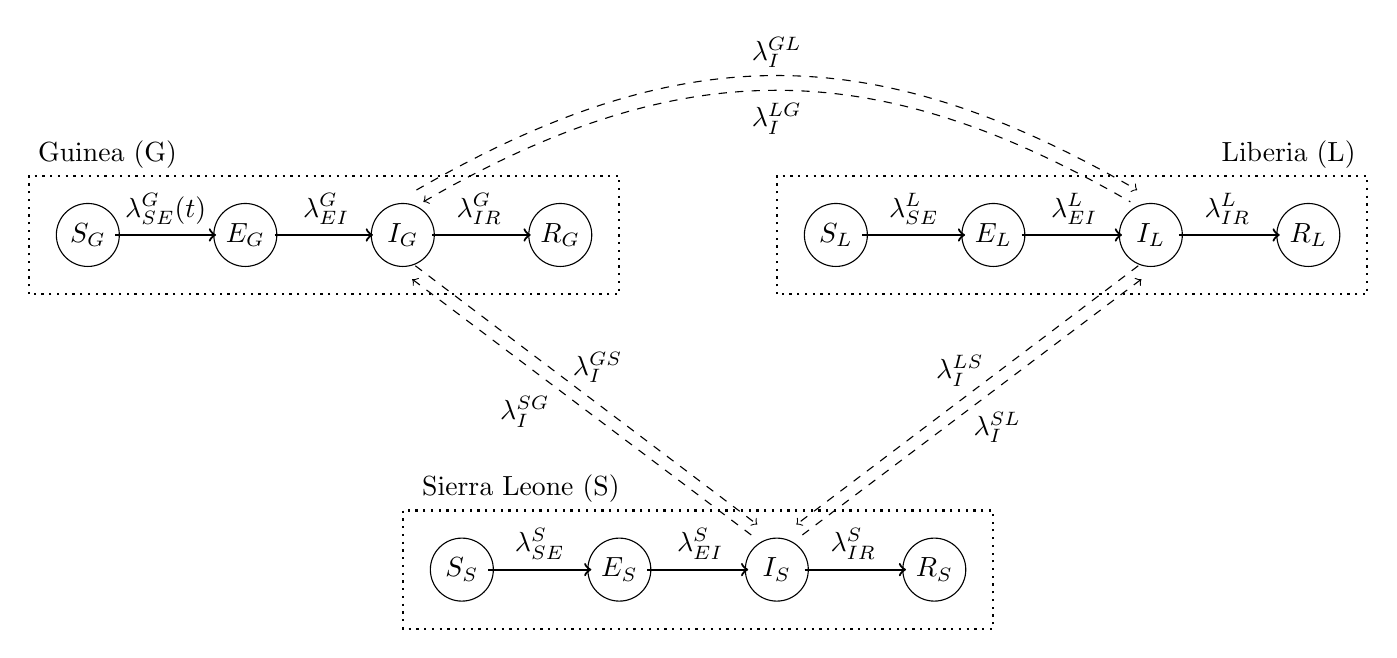
\begin{tikzpicture}
		\draw[thick,dotted] (0,-0.25) rectangle (7.5, 1.25);
		\node at (1, 1.1) [label=Guinea (G)] {};
		\draw (0.75, 0.5) circle(0.4) node (Sa) {$ S_G $};
		\draw (2.75, 0.5) circle(0.4) node (Ea) {$ E_G $};
		\draw (4.75, 0.5) circle(0.4) node (Ia) {$ I_G $};
		\draw (6.75, 0.5) circle(0.4) node (Ra) {$ R_G $};
		
		\draw[thick,dotted] (9.5,-0.25) rectangle (17, 1.25);
		\node at (16, 1.1) [label=Liberia (L)] {};	
		\draw (10.25, 0.5) circle(0.4) node (Sb) {$ S_L $};
		\draw (12.25, 0.5) circle(0.4) node (Eb) {$ E_L $};
		\draw (14.25, 0.5) circle(0.4) node (Ib) {$ I_L $};
		\draw (16.25, 0.5) circle(0.4) node (Rb) {$ R_L $};
		
		\draw[thick,dotted] (4.75,-3) rectangle (12.25, -4.5);
		\node at (6.25, -3.15) [label=Sierra Leone (S)] {};	
		\draw (5.5, -3.75) circle(0.4) node (Sc) {$ S_S $};
		\draw (7.5, -3.75) circle(0.4) node (Ec) {$ E_S $};
		\draw (9.5, -3.75) circle(0.4) node (Ic) {$ I_S $};
		\draw (11.5, -3.75) circle(0.4) node (Rc) {$ R_S $};
		
		\draw [thick,->] (Sa) -- (Ea) node[midway,above] {$ \lambda_{SE}^G(t) $};
		\draw [thick,->,shorten >=.6mm] (Ea) -- (Ia) node[midway,above] {$ \lambda_{EI}^G $};
		\draw [thick,->,shorten <=.5mm] (Ia) -- (Ra) node[midway,above] {$ \lambda_{IR}^G $};
		
		\draw [thick,->] (Sb) -- (Eb) node[midway,above] {$ \lambda_{SE}^L $};
		\draw [thick,->,shorten >=.6mm] (Eb) -- (Ib) node[midway,above] {$ \lambda_{EI}^L $};
		\draw [thick,->,shorten <=.5mm] (Ib) -- (Rb) node[midway,above] {$ \lambda_{IR}^L $};
		
		\draw [thick,->] (Sc) -- (Ec) node[midway,above] {$ \lambda_{SE}^S $};
		\draw [thick,->,shorten >=.6mm] (Ec) -- (Ic) node[midway,above] {$ \lambda_{EI}^S $};
		\draw [thick,->,shorten <=.5mm] (Ic) -- (Rc) node[midway,above] {$ \lambda_{IR}^S $};
		
		\path [dashed, <-] ([yshift=-0.5mm,xshift=-2mm]Ia.south) edge [shorten >= 2mm, shorten <= 4mm] node [above,xshift=2.5mm,yshift=1.5mm] {$ \lambda_I^{GS} $} ([xshift=-1mm]Ic.north);
		\path [dashed, ->] (Ia.south) edge [shorten >= 5mm, shorten <= 2mm] node [below,xshift=-9mm,yshift=2mm] {$ \lambda_I^{SG} $} ([xshift=1.5mm]Ic.north);
		
		\path [dashed, <-] ([yshift=-0.5mm,xshift=2mm]Ib.south) edge [shorten >= 2mm, shorten <= 4mm] node[above,yshift=1mm,xshift=-2mm] {$ \lambda_I^{LS} $} ([xshift=1mm]Ic.north);
		\path [dashed, ->] (Ib.south) edge [shorten >= 5mm, shorten <= 2mm] node[below,xshift=5mm] {$ \lambda_I^{SL} $} ([xshift=-1.5mm]Ic.north);
		
		\path [dashed, <-] ([]Ia.north) edge [shorten >= 3mm, shorten <= 3mm, bend left, looseness=1.1] node [below] {$ \lambda_I^{LG} $} ([]Ib.north);
		\path [dashed, ->] ([]Ia.north) edge [shorten >= 2mm, shorten <= 2mm, bend left, looseness=1.1,yshift=2mm] node [above] {$ \lambda_I^{GL} $} ([]Ib.north);	
		\end{tikzpicture}
	}
	\caption[Model diagram for a stratified SEIR model with country specific outbreak dynamics and cross--country virtual transmission.]{Diagram of state transitions for a stratified SEIR model used in simulating an outbreak in Guinea, Liberia, and Sierra Leone. Dashed boxes denote countries, nodes in circles denote the model compartments: susceptible (S), exposed (E), infectious (I), recovered (R). Compartments  are subscripted with country indicators. Solid lines with arrows indicate stochastic transitions between model compartments, which occur continuously in time. Dashed lines indicate virtual migrations, where infected individuals in one country contribute to the force of infection in another country but do not migrate. Rates at which individuals transition between compartments are denoted by $ \lambda $ and are subscripted by compartments and superscripted by countries, e.g., $ \lambda_{SE}^L $ is the rate at which susceptible individuals become exposed in Liberia, $ \lambda_I^{SG} $ is the rate at which an infected individual in Sierra Leone migrates to Guinea. The rate at which susceptibles in Guinea become infected is time varying with one changepoint at 33 weeks. Full expressions for the rates are given in Table \ref{tab:ebola_synth_rates_full}.}
	\label{fig:stratified_seir_approx_diag}
\end{figure}

We should be aware that not all the parameters in this model are identifiable from the data, although in this case it happens that all the parameters are captured in the posterior (see Figure ((((insert figure number))))). We discuss in Section \ref{sec:est_scale_discussion} that the effective population sizes are not separately identifiable from the mean case detection probabilities. Rather, the mean case detection rate, $ \rho N_{eff} $, is well estimated because of its relationship to the true and observed final outbreak sizes. We also rely on priors to quantify our uncertainty about other aspects of the transmission dynamics, such as the rates of infectious contact from other countries and the ratio of the infectious to latent period duration. For these parameters, the posterior essentially reflects the prior. We emphasize that, in our view, adopting informative priors that reflect reasonable scales for unidentified parameters is strongly preferable to the common approach of fixing these parameters. If they are not estimable from the data, we have no business expressing absolute certainty about their values!

((((Insert posterior histograms when regenerated))))



\section{Application: Modeling the Spread of Ebola}
\label{sec:lna_ebola} % linear noise approximation
\chapter{Models with Time--Varying Dynamics for Pandemic A(H1N1) Influenza in Finland}
\label{chap:lna_extensions}

\section{Overview}
\label{sec:lna_extensions_overview}
To this point, we have largely worked with stochastic epidemic models (SEMs) where the transmission dynamics of an outbreak are time--homogeneous. This may be only mildly unreasonable for short outbreaks in closed, relatively ``well--mixed" populations, and is often an attractive modeling choice as SEMs with static dynamics are easier to interpret and fit. Incidence data typically arise in settings where the outbreak milieu changes with environmental factors, heterogeneity in the contact structures of various subpopulations as they are exposed, or behavioral responses as people become aware of an outbreak (or complacent about the extent to which it is under control). Furthermore, we are often interested in understanding the effects of time--varying interventions, such as vaccination campaigns, on the transmission dynamics of an outbreak. Thus, it is important to allow time--varying aspects of an outbreak to be flexibly expressed in the model.

In this chapter, we will use SEMs with time--varying force of infection (FOI) to model the spread of pandemic A(H1N1) influenza in Finland using surveillance data. Our goals will be to quantify the transmission dynamics of the outbreak, to estimate the true incidence, and to understand what effect a national vaccination campaign had in mitigating the outbreak severity. We will use the LNA and ODE SEM representations to fit models with time--varying dynamics. 

%We will compare models with time--varying and constant dynamics that we fit using the linear noise approximation (LNA) framework developed in Chapter \ref{chap:lna_for_sems}.

\subsection{On the Importance of Allowing for Time--Varying Dynamics}
\label{subsec:tparam_motivation}

A critical aspect of modeling outbreaks over multiple seasons is that we must account for changes in rates of infectious contacts both within, and between, seasons. The decline in transmission at the end of one season may be attributable, in some combination, to stochastic extinction, a decline in the rate of infectious contact, and a reduction in the effective number of susceptible individuals via immunity acquired from natural exposure or vaccination. It is difficult to explain the emergence of the second season without allowing for stochastic reemergence, changes in the FOI, or waning immunity. Put another way, it is highly unlikely an outbreak that died off in a population protected by herd immunity would reemerge absent changes in FOI or repletion of susceptibles in the population. 

Before delving into details of how we intend to accommodate time--inhomogeneity in the FOI, we briefly highlight why we should bother. To make the point, we compare results for two SIRS models fit to incidence data from an outbreak with time--inhomogeneous dynamics. The data were simulated from an SIRS model where the rate of infectious contact varied sinusoidally over the course of two waves (depicted in Figure \ref{fig:sinfoi_tparam_plots}). While both models allowed for loss of immunity, the per--contact infectious rate was held constant in one model, and in the other was allowed to vary in time, with changes penalized via a first order Gaussian Markov random field (GMRF) shrinkage prior (details presented in Sections \ref{sec:flu_tparam_models} and \ref{sec:tparam_motiv_details}). We used the LNA framework developed in Chapter \ref{chap:lna_for_sems} to fit both models. 

Although both models are misspecified vis--a--vis the  data generating model, the model with time--varying FOI was clearly better able to describe the dynamics of the outbreak (Figure \ref{fig:sinfoi_tparam_plots}). Estimates of basic and effective reproduction numbers capture the true basic and effective reproduction numbers throughout both seasons. The model with time--varying FOI is also able to recover the true incidence. In contrast, the model with constant FOI fails to accurately estimate the basic and effective reproduction numbers between seasons and during the second wave. It also completely fails to capture the incidence during the second wave. Unlike the model with time--varying FOI, the model with constant FOI also fails to recover the hyperparameters governing the outbreak dynamics and sampling process. In particular the mean duration of immunity and case detection rate are important parameters that are poorly estimated (Figure \ref{fig:sinfoi_param_plots}). Finally, the posterior predictive distributions for the model with time--varying FOI are more accurate, and more precise, than posterior predictive distributions for the model with constant FOI (Figures \ref{fig:sinfoi_tparam_plots} and \ref{fig:sinfoi_ppi_comp}).

\begin{figure}[htbp]
	\centering
	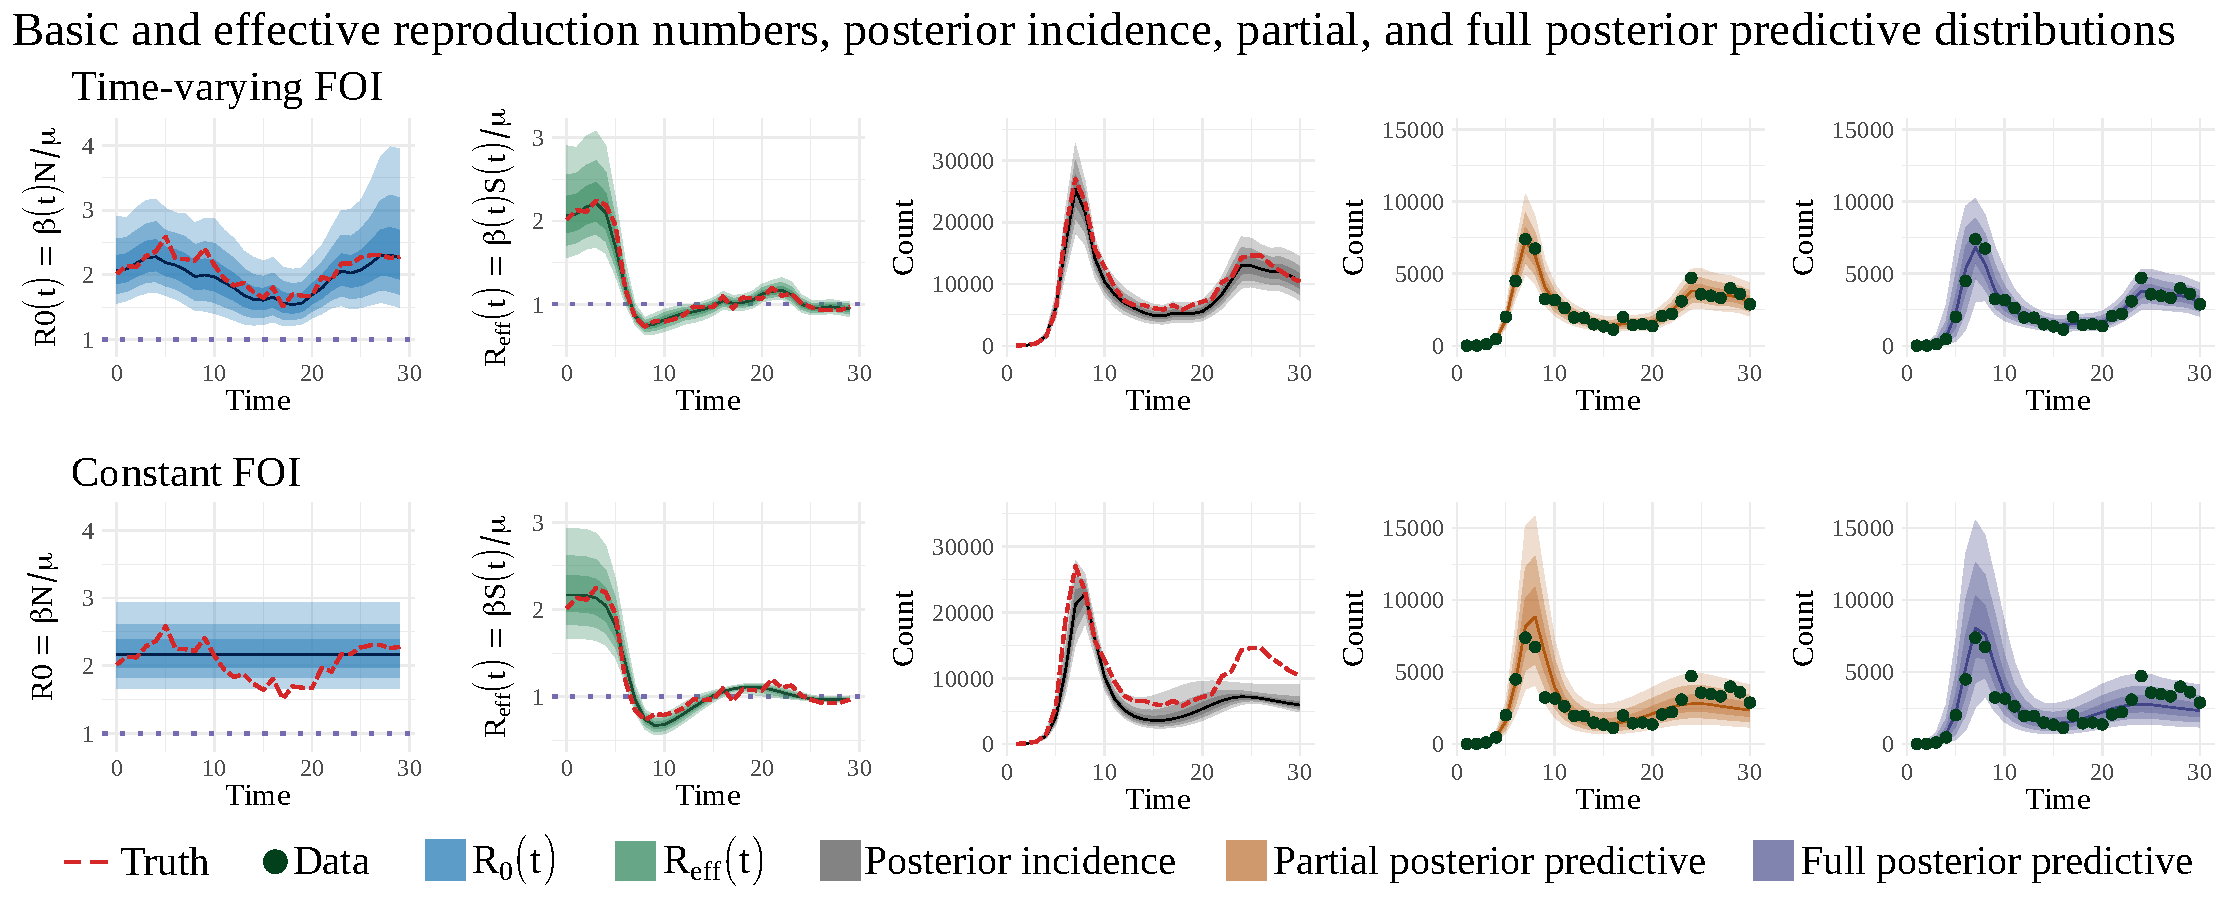
\includegraphics[width=\linewidth]{figures/sinfoi_lna_tparam_plots}
	\caption[Time--varying reproduction numbers, latent incidence, and posterior predictive distributions for SIRS models fit to data from an outbreak with time--varying dynamics.]{From left to right: posterior distributions of basic reproduction numbers, of effective reproduction numbers, of latent incidence, partial and full posterior predictive distributions. The top row corresponds to estimates obtained using an SIRS model where the basic reproduction number, and hence the per--contact infectivity rate, was allowed to vary in time, with differences penalized according to a first order GMRF. The second row shows estimates obtained from an SIRS model where the per--contact infectivity rate was constant over time. Shaded bands correspond to pointwise 50\%, 80\%, and 95\% Bayesian credible intervals and posterior predictive intervals, with the pointwise posterior/predictive median drawn as a solid line of the corresponding color.}
	\label{fig:sinfoi_tparam_plots}
\end{figure}

\begin{figure}[htbp]
	\centering
	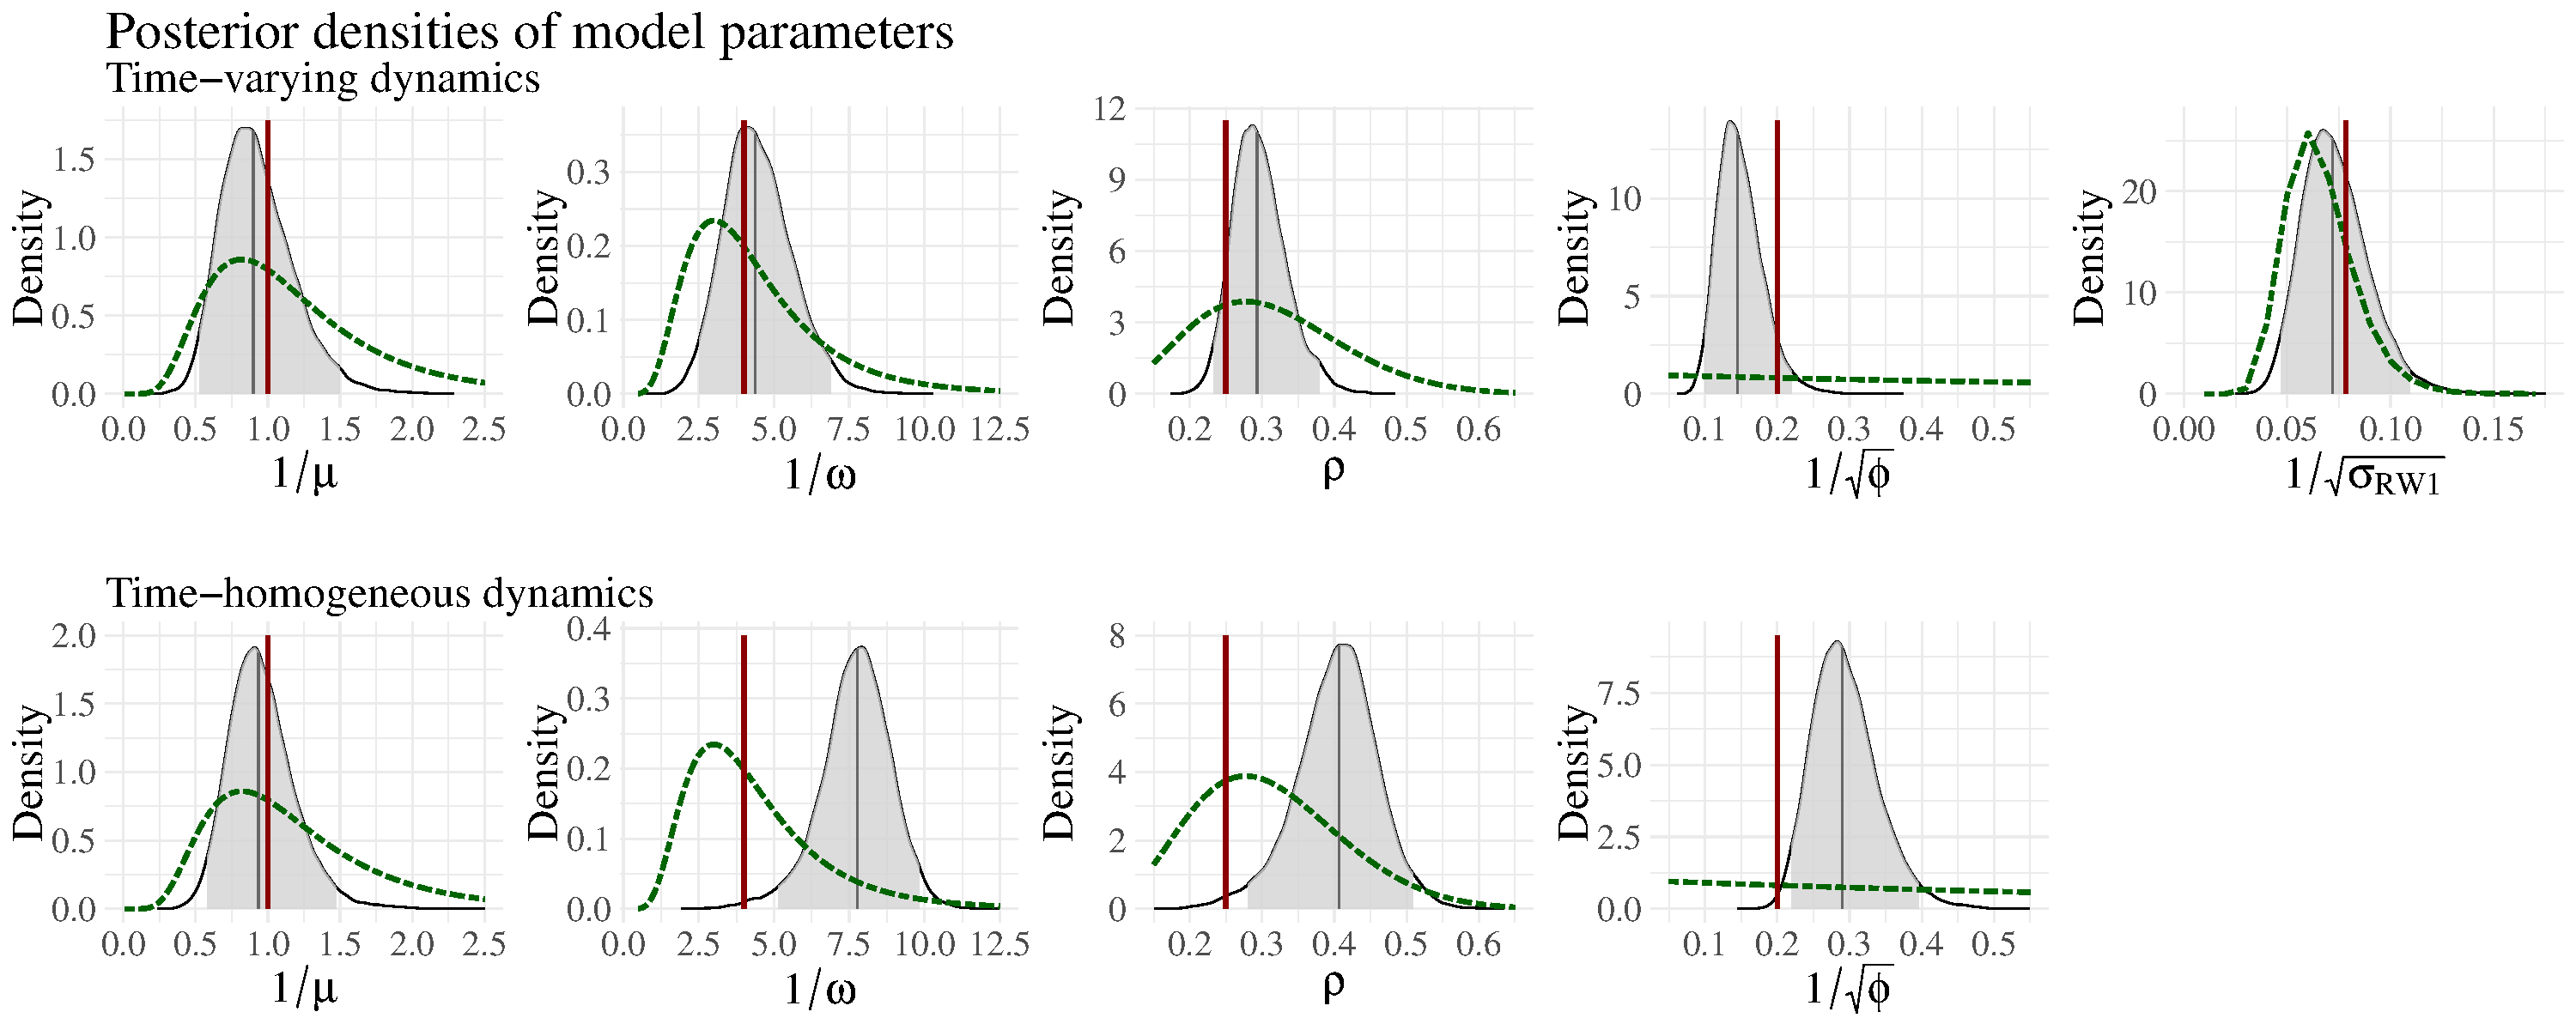
\includegraphics[width=\linewidth]{figures/sinfoi_lna_param_plots}
	\caption[Posterior distributions of SIRS model parameters fit to data from an outbreak with time--varying dynamics.]{Posterior distributions of SIRS model parameters fit to data from an outbreak with time--varying dynamics. From left to right: $ 1/\mu $, the mean infectious period duration; $ 1/\omega $, the mean duration of immunity; $ \rho $, the mean case detection rate; $ \phi $, negative binomial overdispersion parameter; $ \sigma_{RW1} $, standard deviation of log--differences of time--varying basic reproduction numbers. The true values are given by solid red lines and priors by dashed green curves. The solid grey lines are posterior medians, and shaded regions correspond to 95\% Bayesian credible intervals.}
	\label{fig:sinfoi_param_plots}
\end{figure}

\begin{figure}[htbp]
	\centering
	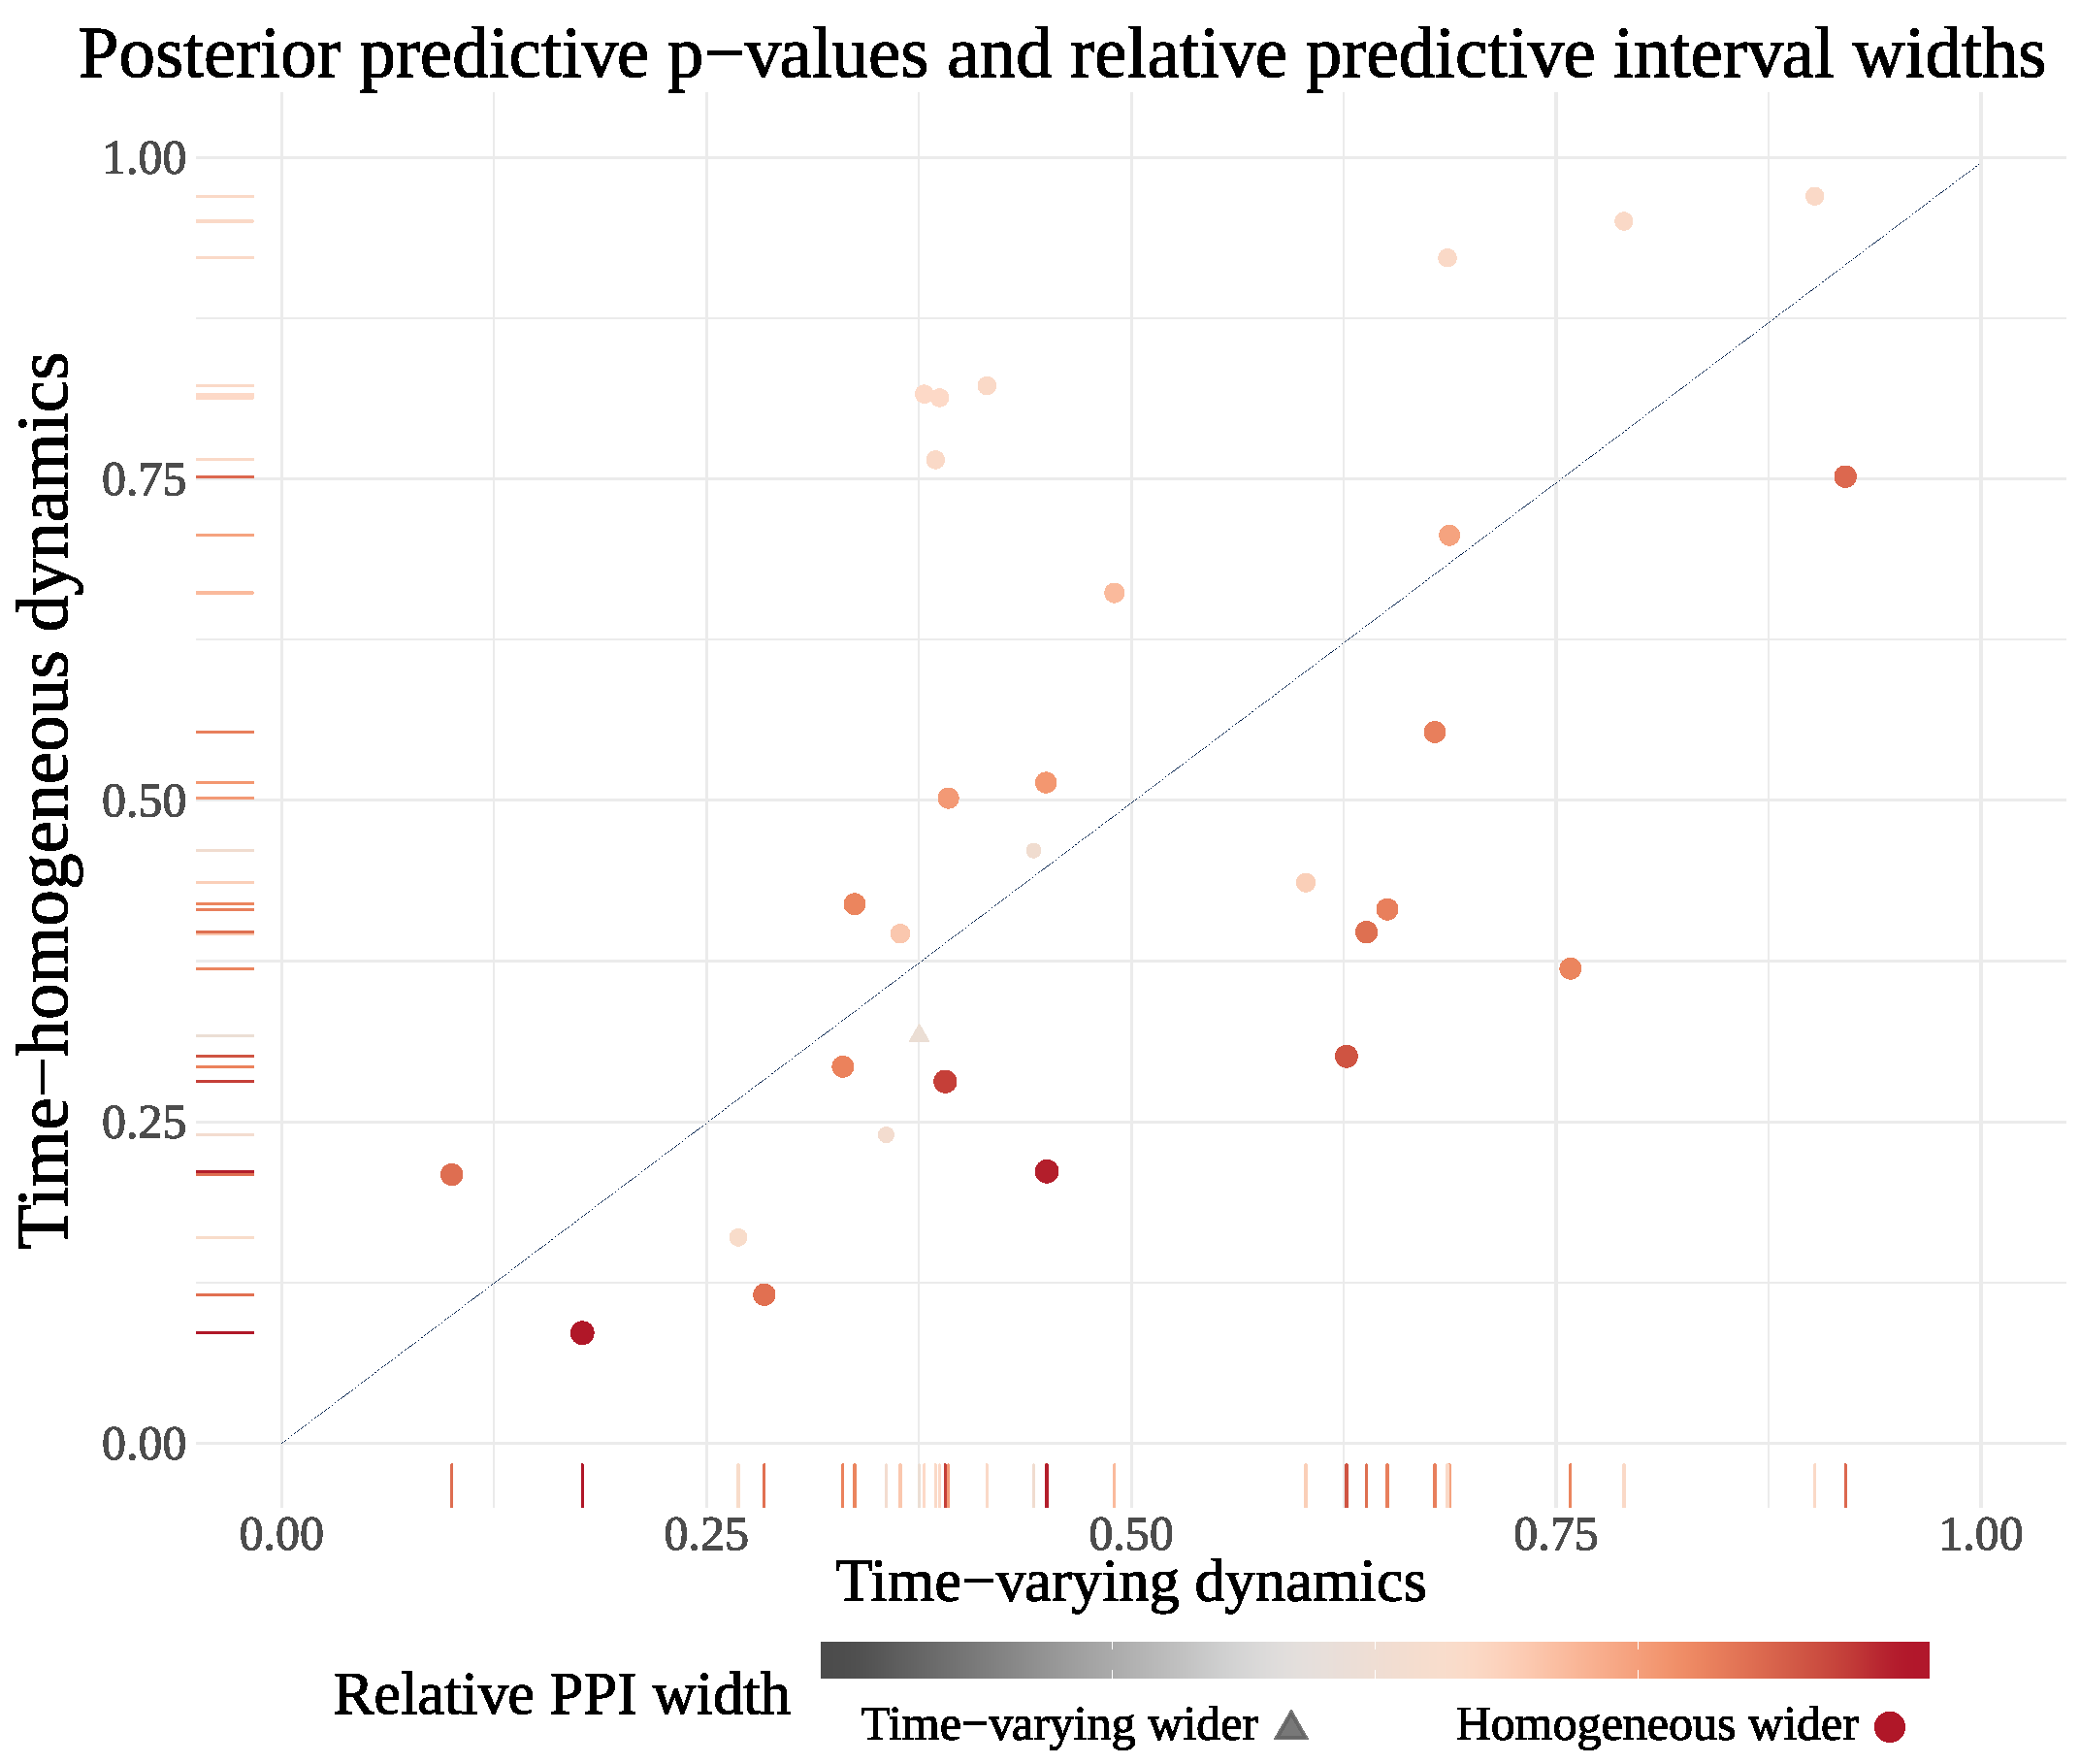
\includegraphics[width=0.6\linewidth]{figures/sinfoi_ppi_comp}
	\caption[Comparison with posterior predictive p-values and relative predictive interval widths for SIRS models fit to an outbreak with time--varying dynamics.]{Comparison of models with time--varying and constant force of infection using posterior predictive p-values (PPPs) and relative posterior predictive interval (PPI) widths. Each point corresponds to the observed incidence in a given week. The X--Y coordinates give the PPPs under a model with a time--varying force of infection (FOI), where R0 was modeled as a Gaussian Markov random field of order one, the PPP under a model with constant per--contact infection rate. The size and color of each point corresponds to the relative PPI width, computed as $ (\widehat{\sigma}_{post,\ell}^{constant} - \widehat{\sigma}_{post,\ell}^{RW1})/\widehat{\sigma}_{post,\ell}^{RW1} $, and the sign of the relative width is further emphasized by the shape of the point. Dots indicate that PPIs with constant FOI are wider, the lone triangle corresponds to the one data point where the PPI for the model with time--varying FOI was wider.}
	\label{fig:sinfoi_ppi_comp}
\end{figure}

\newpage
\section{Modeling the Spread of A(H1N1)pdm09 in Finland}
\label{sec:flu_tparam_models}

\subsection{Data and Vaccination}
\label{subsec:flu_datavacc}

We will model the time series of weekly incidence among youths (Y), ages 0--19, and adults (A), ages 20+, over a one year period beginning in epiweek 15, 2009, one month prior to the first observed case in the first season, and a 42 week period beginning in epiweek 33, 2010, corresponding to the start of the 2010--2011 Finnish school year \cite{calendarFinland}. Data from the inter--season period, epiweeks 15--32, 2010, were aggregated over the inter--season period and indexed at epiweek 33, 2010. We denote the data as, $$ \bY = \left (\left (Y_{Y,1},Y_{A,1}\right ),\dots,\left (Y_{Y,52},Y_{A,52}\right ),\left (Y^\prime_{Y,71},Y^\prime_{A,71}\right ),\dots,\left (Y_{Y,113},Y_{A,113}\right )\right ), $$ where the index corresponds to weeks elapsed from week zero, i.e., epiweek 15, 2009. The observed incidence in age--stratum $ j $ at week $ \ell $ is modeled as a negative binomial sample of the true incidence \begin{equation}
\label{flu_emit_prob}
Y_{j,\ell} \sim \mr{Neg.Binom}\left (\mu = \rho_j(\Delta N_{SI}^{(u)}(t_\ell) + \Delta N_{SI}^{(v)}(t_\ell)), \sigma^2 = \mu + \mu^2 / \phi_j\right ),
\end{equation}
where $ \rho_j $ is the age--specific mean case detection rate, $ \phi_j $ is an age--specific overdispersion parameter, and $ \Delta $ is a differencing operator for the cumulative incidence in a age--vaccination stratum, e.g., $ \Delta N_{SI}^{(u)}(t_\ell) = N_{SI}^{(u)}(t_\ell) - N_{SI}^{(u)}(t_{\ell-1}) $ is change in cumulative incidence between times $ t_{\ell-1} $ and $ t_\ell $. Note that the time--step for the data and incidence over the inter--season period is twenty weeks long. 

\begin{sidewaysfigure}[htbp]
	\centering
	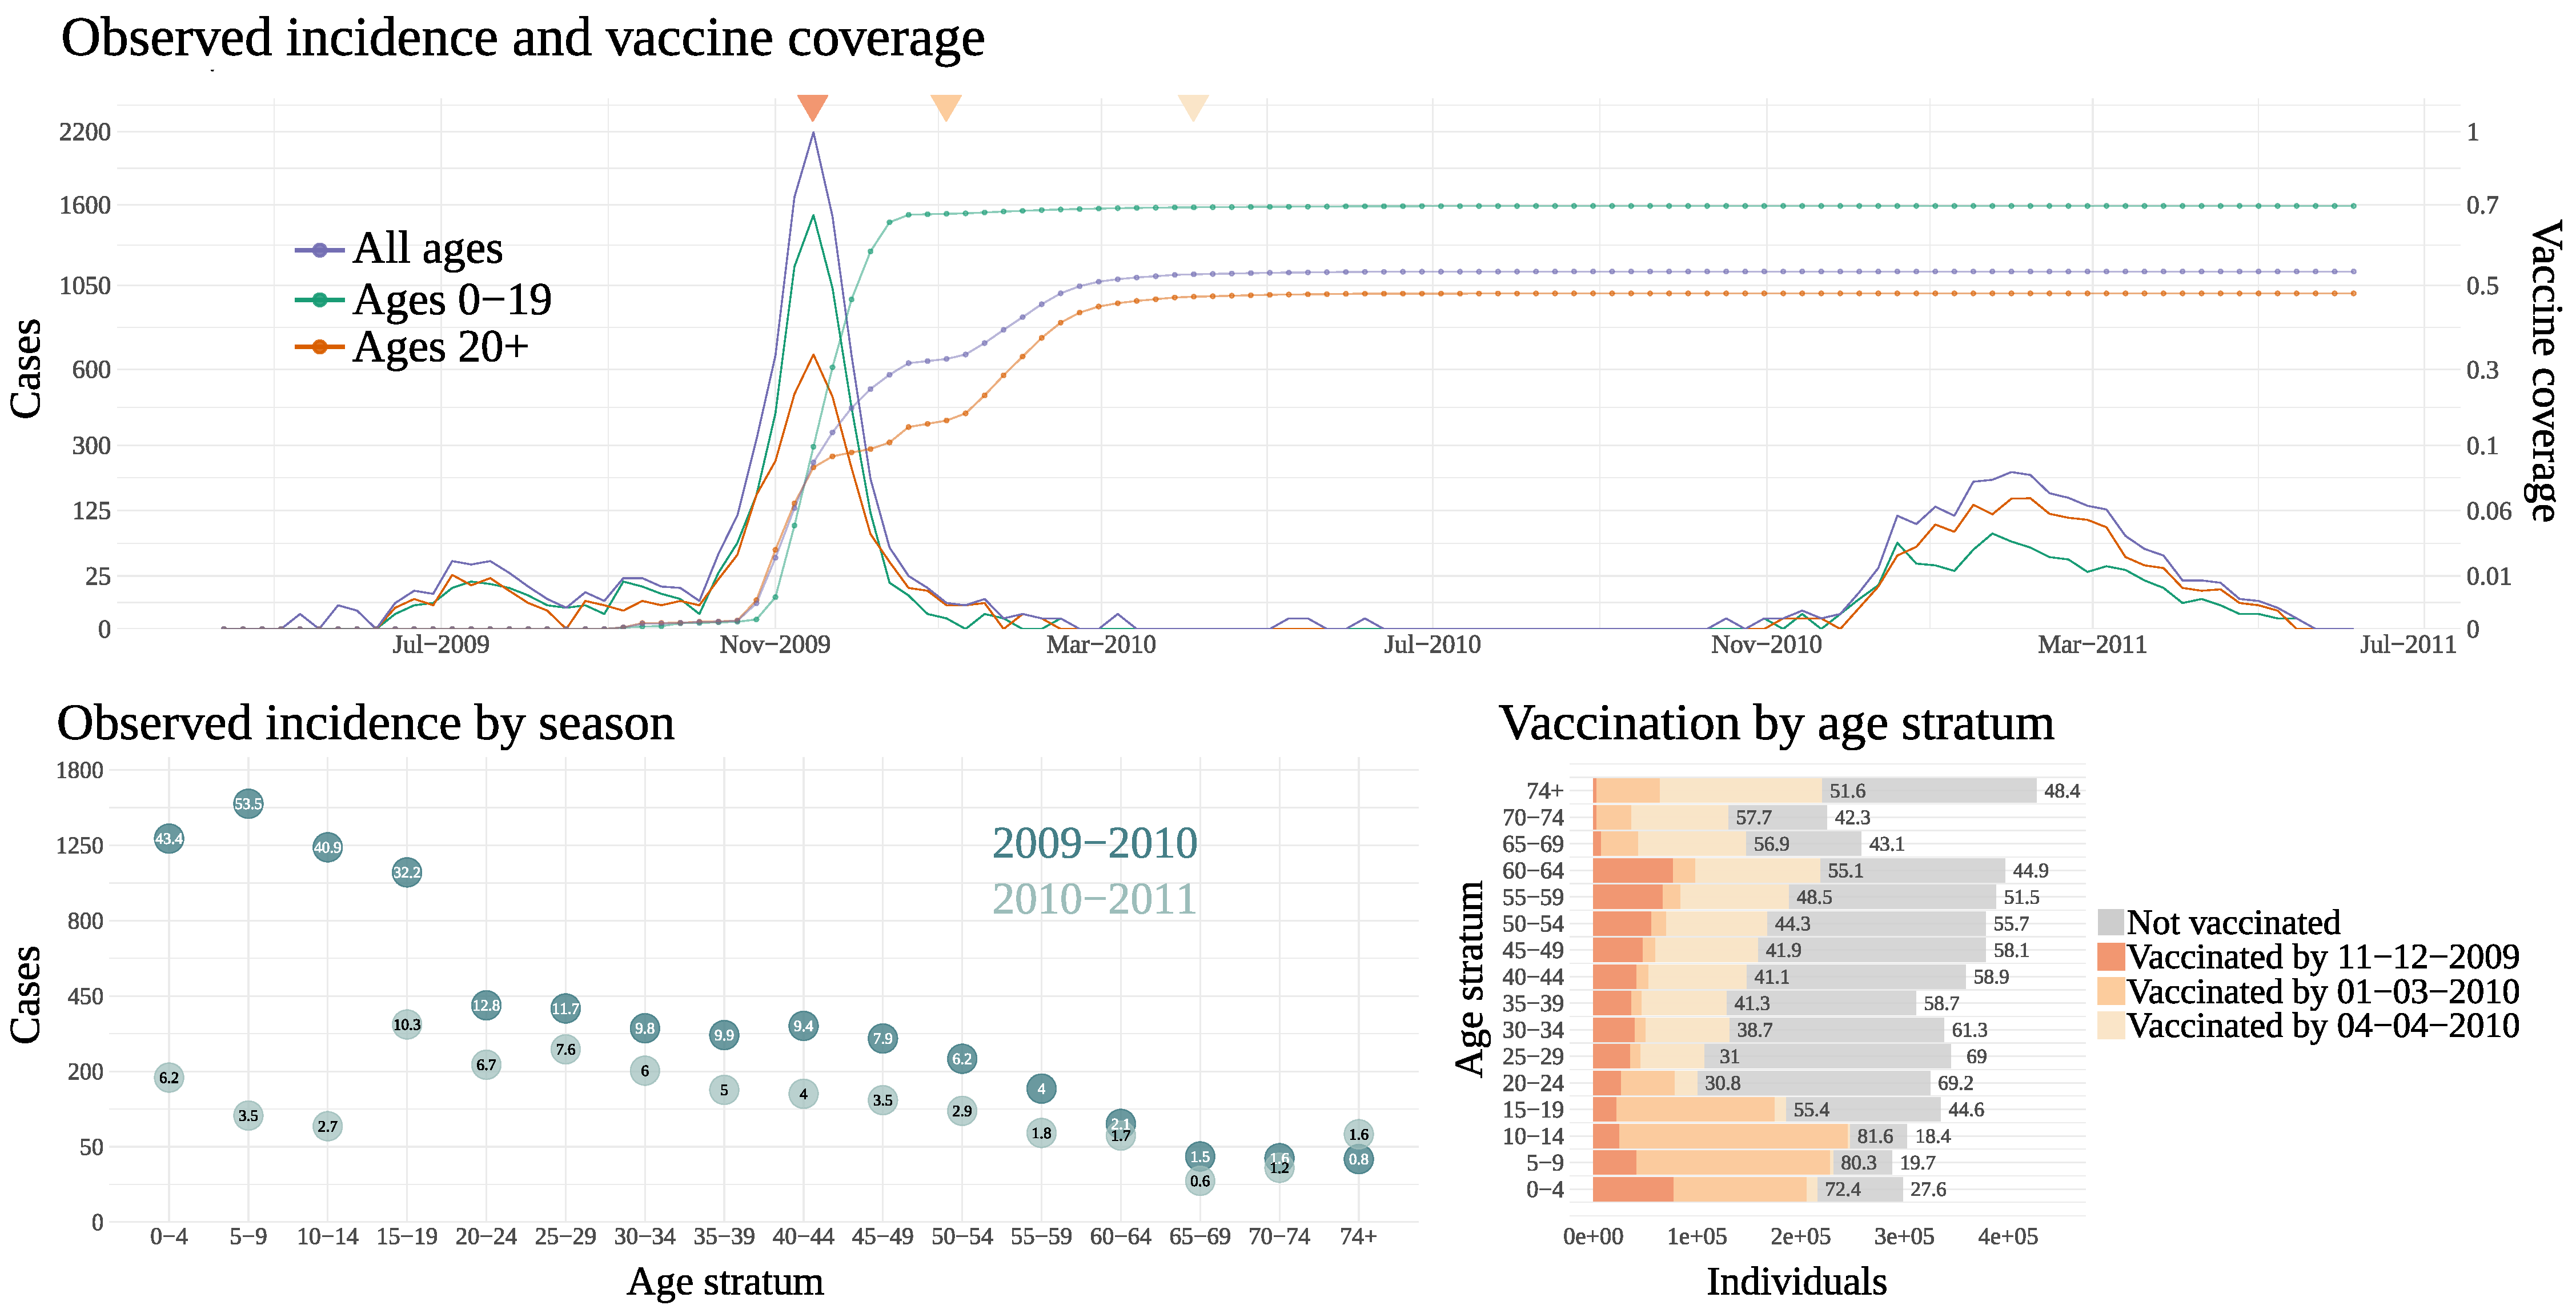
\includegraphics[width=\linewidth]{figures/fludat_plots}
	\caption[A(H1N1)pdm09 incidence and vaccination data from Finland, April 15, 2009 --- June 5, 2011.]{(Top) Observed incidence (solid lines) and vaccine coverage (lines with points). (Bottom left) Observed cases by season and age stratum. The 2009--2010 season (dark green) corresponds to the period from April 15, 2009 through April 4, 2010. The 2010--2011 season (light green) corresponds to the period from September 12, 2010 through June 5, 2011. Numbers in points give the attack rate within each stratum for the corresponding season. (Bottom right) Vaccination coverage by age stratum, colored by vaccine coverages at the times of peak incidence in the first season, tail of the major outbreak in the first season, and end of the vaccination campaign. The numbers inside and outside the histograms denote the percentage of individuals in each stratum that were vaccinated and unvaccinated, respectively, by the end of the vaccination campaign. The times at which vaccine coverages are summarized, denoted by colors of histogram bars, are also identified by corresponding triangles above the top figure.}
	\label{fig:finland_fludat}
\end{sidewaysfigure}

\subsection{Model Structure}
\label{subsec:flu_modstructure}

We fit an age--vaccination stratified susceptible--infected--recovered--susceptible (SIRS) model in which individuals transition stochastically, and continuously in time, between disease states. Individuals are assumed to become infectious immediately upon becoming infected, and acquire temporary, though potentially long lasting, protection upon recovery. Individuals who lose immunity are assumed to become fully susceptible. Following \cite{shubin2016revealing}, we assume a closed population and ignore demographic changes or mortality. All individuals were assigned to be susceptible and unvaccinated at the start of the modeling period. The model is diagrammed in Figure \ref{fig:flu_sirs_diag}, and Table \ref{tab:flu_notation} lists the model parameters and their interpretations. 

\begin{table}[htbp]
	\caption{Summary of notation for influenza models.}
	\label{tab:flu_notation}
	\footnotesize
	\centering
	\begin{tabular}{llc}
		\hline
		\textbf{Parameter} & \textbf{Interpretation} & \textbf{Time--varying}\\
		\hline
		$\alpha_j(t)$ & Rate of exogenous infectious contact, age stratum $ j $ & Yes \\
		$ \beta_j(t) $ & Per--contact rate of endogenous infection, age stratum $ j $ & Yes \\
		$ \nu $ & Rel. rate of infectious contact for vaccinated ($ 1- $VE for susceptibility) & No \\
		$1/\mu_j$ & Mean infectious period duration, age stratum $ j $ & No\\
		$ 1/\omega $ & Mean duration of immunity & No \\
		$ \rho_j $ & Mean case detection rate, age stratum $ j $ & No\\
		$ \phi_j $ & Negative binomial overdispersion parameter, age stratum $ j $ & No \\
		$ \bX(t) $ & Compartment counts at time $ t $ & Yes\\
		$ \bN(t) $ & Cumulative incidence by time $ t $ & Yes \\
		\hline \hline
		\textbf{Variable} & \textbf{Interpretation} & \textbf{Time-varying}\\
		\hline		
		$ Y_{j,\ell} $ & Observed incidence, age stratum $ j $, time $ t_\ell $ & Yes \\
		$ \mathcal{T} $ & Observation times, numbered by week:  $ \lbrace t_\ell:\ \ell=1,\dots,52,71,\dots,113\rbrace $& No \\
		$ N$ & Population size & No\\
		$ N_{j}^{(k)}(t_\ell) $ & Size of age stratum $ j $ with vaccination status $ k $ in week $ \ell $ & Yes \\
		$ V_{j}(t_\ell) $ & \# vaccine doses to individuals in age stratum j at week $ \ell $ & Yes\\	
		$ P^v_{j}(t_\ell) $ & Vaccination coverage in age stratum $ j $ by week $ \ell $ & Yes \\
		$ \xi_{k,j}^{(uv)}(t_\ell) $ & Vaccination forcing for compartment $ k $ in age stratum $ j $ in week $ \ell $ & Yes\\
		$ C_{jk} $ & Relative contact rate to age stratum $ j $ from stratum $ k $ & No\\
		$ R_0(t) $ & Basic reproduction number at time $ t $ & Yes \\
		$ R_{eff}(t) $ & Effective reproduction number at time $ t $ & Yes \\
		$ T_{0,j}(t) $ & Basic type reproduction number at time $ t $, stratum $ j $ & Yes \\
		$ T_{eff,j}(t) $ & Effective type reproduction number at time $ t $, stratum $ j $ & Yes \\
		$ \psi_j(t) $ & Intrinsic reproduction number at time $ t $, stratum $ j $ & Yes\\
		\hline
	\end{tabular}
\end{table}

By taking the sojourn time in each disease state to be exponentially distributed, and leveraging the exchangeability of individuals within the model, we represent the time--evolution of the epidemic as a Markov jump process (MJP), $$ \bX^c = \lbrace S_{Y}^{(u)}, I_{Y}^{(u)}, R_{Y}^{(u)},
S_{Y}^{(v)}, I_{Y}^{(v)}, R_{Y}^{(v)}, S_{A}^{(u)}, I_{A}^{(u)}, R_{A}^{(u)},
S_{A}^{(v)}, I_{A}^{(v)}, R_{A}^{(v)} \rbrace, $$ on the state space of compartment counts, $ \mcS_X^c$, with corresponding cumulative incidence process $ \bN^c $ on the state space of cumulative incidence counts $ \mcS_N^c $.

\begin{figure}[htbp]
	\centering
	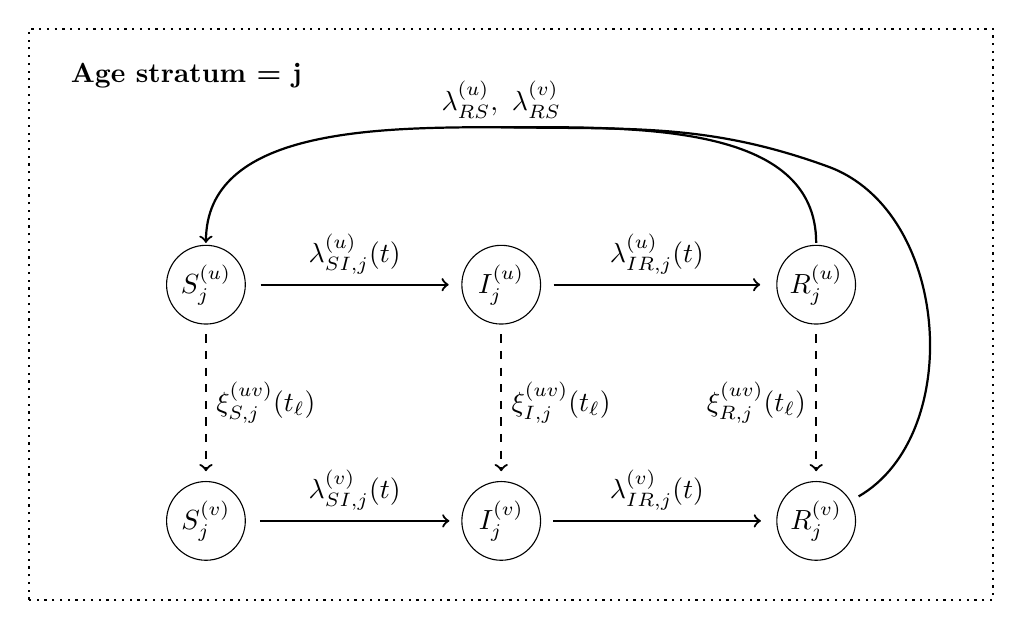
\begin{tikzpicture}
	\draw[thick,dotted] (-1,1) rectangle (11.25,8.25);
	\node at (1,7.25) [label={\textbf{Age stratum = j}}] {};
	\draw (1.25,5) circle(0.5) node (Sju) {$S_j^{(u)}$};
	\draw (5,5) circle(0.5) node (Iju) {$I_j^{(u)}$};
	\draw (9,5) circle(0.5) node (Rju) {$R_j^{(u)}$};
	\draw (1.25,2) circle(0.5) node (Sjv) {$S_j^{(v)}$};
	\draw (5,2) circle(0.5) node (Ijv) {$I_j^{(v)}$};
	\draw (9,2) circle(0.5) node (Rjv) {$R_j^{(v)}$};
	\draw (5,7) coordinate (rec) {};
	\draw (5,7.35) node (reclab) {$ \lambda_{RS}^{(u)},\ \lambda_{RS}^{(v)} $};
	\draw (9.15,6.5) coordinate (rec2) {};
	
	\draw [thick,shorten >=0.25cm,shorten <=0.25cm,->] (Sju) -- (Iju) node[midway,above] {$ \lambda_{SI,j}^{(u)}(t) $};
	\draw [thick,shorten >=0.25cm,shorten <=0.25cm,->] (Iju) -- (Rju) node[midway,above] {$ \lambda_{IR,j}^{(u)}(t) $};
	\draw [thick,shorten >=0.25cm,shorten <=0.25cm,->] (Sjv) -- (Ijv) node[midway,above] {$ \lambda_{SI,j}^{(v)}(t) $};
	\draw [thick,shorten >=0.25cm,shorten <=0.25cm,->] (Ijv) -- (Rjv) node[midway,above] {$ \lambda_{IR,j}^{(v)}(t) $};
	
	\draw [dashed,thick,shorten >=0.25cm,shorten <=0.25cm,->] (Sju) -- (Sjv) node[midway,right] {$ \xi_{S,j}^{(uv)}(t_\ell) $};
	\draw [dashed,thick,shorten >=0.25cm,shorten <=0.25cm,->] (Iju) -- (Ijv) node[midway,right] {$ \xi_{I,j}^{(uv)}(t_\ell) $};
	\draw [dashed,thick,shorten >=0.25cm,shorten <=0.25cm,->] (Rju) -- (Rjv) node[midway,left] {$ \xi_{R,j}^{(uv)}(t_\ell) $};
	
	\draw [thick,shorten >=0cm,shorten <=0.15cm] (Rju) to [out=90, in = 0] (rec);
	\draw [thick,shorten >=0cm,shorten <=0.1cm] (Rjv) to [out=30, in = -20] (rec2);
	\draw [thick] (rec2) to [out=160,in=-1] (rec);
	\draw [thick,shorten >=0.15cm,shorten <=0.0cm,->] (rec) to [out=180, in = 90] (Sju);
	\end{tikzpicture}
	\caption[Diagram of state transitions for an age--vaccination stratified SIRS model for influenza.]{Diagram of state transitions for an age--vaccination stratified SIRS model for influenza in Finland. Both age strata, 0--19 and 20+, have the same compartmental structure. Nodes in circles denote model compartments, which are subscripted with age stratum and superscripted with vaccination status. Solid lines indicate stochastic transitions that occur continuously in time. Rates of disease state transitions, denoted by $ \lambda $, are subscripted with the states from which, and to which, individuals flow and by the age stratum. Superscripts for transition rates indicate vaccination status. Dashed lines represent deterministic forcings from unvaccinated to vaccinated compartments that occur at discrete times. The mass of the forcing at time $ t $, denoted $ \xi(t) $, is subscripted by the compartment and age stratum, and superscripted by the direction of the forcing (unvaccinated to vaccinated).} 
	\label{fig:flu_sirs_diag}
\end{figure}

The contact rate between individuals in age stratum $ j $ and age stratum $ k $, denoted $ C_{jk} $, was based on estimated mean contact rates, appropriately standardized (see Section \ref{sec:flu_contact_rates}), from the Finnish arm of the POLYMOD survey \cite{mossong2008social,polymod} and accessed via the \texttt{socialmixr R} package \cite{funk2018socialmixr}. Sixty percent of contacts in the 0--19 age group were from other individuals age 0--19, while eighty--five percent of the contacts in the 20+ age group were from other adults.  The rates, $ \blambda = (\blambda_{Y},\blambda_{A}) $, at which individuals in age--stratum $ j \in \lbrace Y,\ A\rbrace $ transition between disease states are
\begin{equation}\small
\label{eqn:flu_sirs_rates}
\blambda_{j} = \left\lbrace
\begin{array}{ll}
\lambda_{SI,j}^{(u)} = \left [\alpha_{j}(t) + \beta_{j}(t)\left (C_{jk}\left (I_{j}^{(u)} + I_{j}^{(v)}\right ) + (1-C_{jk})\left (I_{k}^{(u)} + I_{k}^{(v)}\right )\right )\right ]S_{j}^{u} \\ 
\lambda_{SI,j}^{(v)} = \nu\left [\alpha_{j}(t) + \beta_{j}(t)\left (C_{jk}\left (I_{j}^{(u)} + I_{j}^{(v)}\right ) + (1-C_{jk})\left (I_{k}^{(u)} + I_{k}^{(v)}\right )\right )\right ]S_{j}^{v}\\
\lambda_{IR,j}^{(u)} = \mu_{j} I_{j}^{(u)} \\
\lambda_{IR,j}^{(v)} = \mu_{j} I_{j}^{(v)} \\
\lambda_{RS,j}^{(u)} = \omega R_{j}^{(u)} \\
\lambda_{RS,j}^{(v)} = \omega R_{j}^{(v)}
\end{array}
\right .
\end{equation}

At weekly intervals, we deterministically force individuals from unvaccinated model compartments to the corresponding vaccinated compartments. Following \cite{shubin2016revealing}, we assume that vaccine doses were distributed proportionally to the number of individuals in each unvaccinated compartment of the corresponding age stratum. In \cite{shubin2016revealing}, it was assumed that vaccination was fully protective with 80\% probability two weeks after administration. Here, we will assume that the vaccine is partially protective in that it reduces the rate at which vaccinated individuals become infected. We do not assume that VE for susceptibility varies by age, and also do not model vaccine efficacy for infectiousness or recovery due to the limited extent of the data. To account for the time required to elicit an immune response, we apply the deterministic forcing at the beginning of week after the time when each dose count was indexed. Thus, suppose that at the end of week $ \ell $ we have $ \bX_j^{(u)}(t_\ell) = \left (S_j^{(u)}(t_\ell), I_j^{(u)}(t_\ell), R_j^{(u)}(t_\ell)\right ) $ unvaccinated susceptible, infected, and recovered individuals in age stratum $ j $ and $ \bX_j^{(v)}(t_\ell) = \left (S_j^{(v)}(t_\ell), I_j^{(v)}(t_\ell), R_j^{(v)}(t_\ell)\right ) $ vaccinated individuals, and that $ V_j(t_\ell) $ vaccine doses were recorded for stratum $ j $ in that week. We apply the vaccine forcing to the initial state for the following week: 
\begin{align}
\label{eqn:vacc_forcing}
\begin{split}
	\bX_{j}^{(u)}(t_\ell^+) &= \bX_j^{(u)}(t_\ell) - V_j(t_\ell)\frac{\bX_{j}^{(u)}(t_\ell)}{\sum\bX_{j}^{(u)}(t_\ell)}, \\
	\bX_{j}^{(v)}(t_\ell^+) &= \bX_j^{(v)}(t_\ell) + V_j(t_\ell)\frac{\bX_{j}^{(u)}(t_\ell)}{\sum\bX_{j}^{(u)}(t_\ell)}.
\end{split}
\end{align}
Thus, the vaccination forcing affects the initial condition for the period $ (t_\ell,t_{\ell+1}] $, not the state at time $ t_\ell $. 

The diffusion approximation for the MJP is a real--valued process, $ \bX $, that in its infinite population limit evolves as a deterministic system of ODEs. The state space of $ \bX $ is defined in terms of compartment volumes, $ \mcS_X^R $, and with corresponding cumulative incidence process, $ \bN $, with state space $ \mcS_N^R $. Note that the boundary conditions on the state spaces of $ \bX^c $ and $ \bN^c $, and similarly of $ \bX $ and $ \bN $, ensure positivity of compartment counts and monotonicity of cumulative incidence paths, and that the compartment counts each age--vaccination stratum sum to the number of individuals in that stratum, e.g., $ S_{Y}^{(u)}(t) + I_{Y}^{(u)}(t) + R_{Y}^{(u)}(t) = N_{Y}^{(u)}(t) $. Due to the complexity of the model, we will rely on the deterministic ODE framework that was explored as a comparitor for the LNA in Chapter \ref{chap:lna_for_sems} to facilitate the computation \ref{chap:lna_for_sems}.  

%As in Chapter \ref{chap:lna_for_sems}, we will use the non--centered parameterization of the restarting LNA of the log--transformed SDE to approximate the time--evolution of $ \bX^c $ and $ \bN^c $. Algorithm \ref{alg:doLNA2} details the procedure for mapping standard normal LNA draws onto an LNA sample path with vaccination forcings.

\subsubsection{Reproduction numbers}
\label{subsubsec:stratmod_repnumbs}
The basic reproduction number, $ R_0 $, and its variants describe the propensity of an outbreak to spread through a population \cite{heffernan2005perspectives,van2008further}. $ R_0 $ is loosely interpreted as the average number of secondary infections arising from a single infected individual in a completely susceptible population. An outbreak will fail to sustain itself (almost surely when it evolves deterministically, but in reality with high probability due to the inherently stochastic nature of epidemics) when $ R_0 < 1 $. For this reason, epidemiologists often quantify the effectiveness of a control measure by estimating the extent to which the intervention reduces $ R_0 $. We can interpret the basic reproduction number as an intrinsic reproduction number when there is an exogenous contribution to force of infection \cite{blackwood2018introduction}. From a modeling perspective, is important to understand not only how $ R_0 $ affects the transmission dynamics, but also how various aspects of the model interact to affect $ R_0 $. 

The basic reproduction number of a structured SEM can be obtained by computing the spectral radius (absolute value of the dominant eigenvalue) of the next generation matrix (NGM) for the linearized system of ODEs specifying the flow in and out of states at infection \cite{heffernan2005perspectives,van2017reproduction,van2008further}. The $ i,j $ element of the NGM gives the expected number of secondary infections in age stratum $ i $ given an index infection in stratum $ j $. Noting that vaccinated and unvaccinated invididuals in this model are equally transmissive and have the same mean infectious period durations, we obtain the age--structured next generation matrix
\begin{align}
\label{eqn:sirs_ngm_full}
\bK &= 
	\left (
	\begin{array}{cc}
	K_{YY} & K_{YA} \\
	K_{AY} & K_{AA}
	\end{array}
	\right ) =\left (
	\begin{array}{cc}
	\frac{C_{YY}\beta_Y\left (N_Y^{(u)} + \nu_YN_Y^{(v)}\right )}{\mu_Y} & \frac{C_{YA}\beta_Y\left (N_Y^{(u)} + \nu_YN_Y^{(v)}\right )}{\mu_A} \\[2ex]
	\frac{C_{AY}\beta_A\left (N_A^{(u)} + \nu_AN_A^{(v)}\right )}{\mu_Y} & \frac{C_{AA}\beta_A\left (N_A^{(u)} + \nu_AN_A^{(v)}\right )}{\mu_A}
	\end{array}
	\right ).
\end{align}
The basic reproduction number is 
\begin{align}
\label{eqn:sirs_R0}
R_0 = \frac{1}{2}\left (K_{YY} + K_{AA}\right ) + \frac{1}{2}\sqrt{(K_{YY} - K_{AA})^2 + 4K_{YA}K_{AY}}.
\end{align}

There are a few aspects of this expression that we should highlight. First, it is possible for the outbreak to persist, i.e., $ R_0 > 1 $, even when the intrinsic reproduction number in one of the strata is below 1, e.g., $ K_{YY} <1$. However, a critical aspect of the contact structure is that most of the infectious contacts for each group are within--group contacts ($ C_{YY} = 0.6 $, $ C_{AA}=0.85 $). Therefore, the persistence of an outbreak in both strata suggests that $ K_{11} $ and $ K_{22} $ should not be much less than one. If not, then persistence of the outbreak in the stratum where transmission is not self--sustained implies that either its rate of infectious contact from outside the population is high ($ \alpha_j(t)N_j \gg  1$), and/or that the intrinsic reproduction number in the other stratum is high. This latter possibility could be particularly problematic since it might imply unreasonably high attack rates in the other stratum.

We also note that the basic reproduction number is greater than the average of intrinsic reproduction numbers, $ K_{YY} $ and $ K_{AA} $, since the second term on the right hand side of (\ref{eqn:sirs_R0}) will typically be positive. Similarly, the variance of $ R_0 $ is also greater than the average of variances of $ K_{YY} $ and $ K_{AA} $. For these reasons, we should consider how $ K_{YY} $ and $ K_{AA} $ interact to a prior over $ R_0 $ when parameterizing the model. Note that if the cross--stratum contact rates were negligible, $ R_0 $ would behave like the average of intrinsic reproduction numbers plus a term proportional to the absolute difference between $ K_{YY} $ and $ K_{AA} $. This suggests that prior information about the intrinsic reproduction numbers, either individually (our preference) or about their average and difference, could help identify $ R_0 $. We should also keep in mind that our model is more complicated since the cross stratum terms are not negligible ($ C_{AA} = 0.6 $, $ C_{YY}=0.85 $), hence
\begin{align*}
K_{YA} &= \frac{(1 - C_{YY})}{C_{YY}}\frac{\mu_Y}{\mu_A}K_{YY},\hspace{0.25in}
K_{AY} = \frac{(1 - C_{AA})}{C_{AA}}\frac{\mu_A}{\mu_Y}K_{AA},\\
&\implies K_{YA}K_{AY} = \frac{(1 - C_{YY})(1-C_{AA})}{C_{YY}C_{AA}}K_{YY}K_{AA}.
\end{align*} 
Thus, $ R_0 $ behaves like the average of intrinsic reproduction numbers plus a term that is non--linear in $ K_{11} $ and $ K_{22} $.

Finally we emphasize the importance of accounting for all of the parameters that contribute the intrinsic reproduction numbers, and by extension $ R_0 $, when specifying priors and parameterizing the estimation scale of the MCMC. In particular, it is critical to note that the effective population size might be lower than the nominal population size because of vaccination and depletion of susceptibles. We can easily misspecify the scales of prior distributions for the reproduction numbers, or select an inefficient parameterization for the MCMC estimation scale, by neglecting this dynamic. In our model, for example, the value of $ R_0 $ in the first season, and the rate at which recovered individuals lose immunity, will affect the effective population size at the beginning of the second season. 

\subsection{Flexible Models for the Force of Infection with Gaussian Markov Random Fields}
\label{subsec:flu_gmrf}

We will model the time--varying force of infection using first order GMRFs (random walk of order 1; RW1) for the log intrinsic reproduction numbers and the effective rate of exogenous infectious contacts in each age stratum. The GMRFs are separately specified over three epochs corresponding to the period one month before the first detected case until the start of the Finnish school year in 2009, the beginning of the Finnish school year in 2009 until its start in 2010 (including the inter--season period), and the second epidemic season beginning at the start of the Finnish school year, 2010. These epochs correspond to epiweeks 15, 2009 through epiweek 33, 2009, epiweek 34, 2009 through epiweek 32, 2010, and epiweek 33, 2010 through epiweek 22, 2011. We will assume that the intrinsic reproduction numbers are homogeneous over the inter--season period, from epiweek 16, 2010 -- epiweek 32, 2010.

The GMRF is parameterized on the log scale using a state--space formulation defined by the initial value and first order differences. Let $ \bpsi_{j} = \lbrace\psi_{j,\ell}:\ \ell \in 0,\dots,52,71,\dots,112\rbrace $ be the vector of intrinsic reproduction numbers, ignoring relative contact rates, for stratum $ j \in \lbrace Y,A \rbrace$, and where time is indexed from epiweek 15, 2009. Let $ \bP^v_j = \left (P^v_j(t_1),\dots,P^v_j(t_L)\right )$ denote the vector of vaccine coverage rates for stratum $ j $. Absent vaccination,
\begin{equation}
\label{eqn:R0t_novacc}
\psi^\prime_{j,\ell} = \frac{\beta_j(t_\ell)N_j}{\mu_j},
\end{equation}
where $ \beta(t_\ell) $ is the time--varying rate of infection rate per--endogenous contact, $ \mu_j$ is the recovery rate at week $ \ell $ (season--specific), and $ N_{j} $ is the number of individuals in age stratum $ j $. Accounting for vaccination, 
\begin{equation}
\label{eqn:R0t_vacc}
\psi_{j,\ell} = \frac{\beta_j(t_\ell)N_j\left (1 - P^v_j(t_\ell) + P^v_j(t_\ell)\nu_j\right )}{\mu_j}
\end{equation}
Note that $ \psi_{j,\ell}^\prime = \bpsi_{j,\ell} / \left (1 - P^v_j(t_\ell) + P^v_j(t_\ell)\right ) $. In order to capture the time--varying aspects of the force of infection that are not due to changes in vaccination, we will parameterize the GMRF for the force of infection using (\ref{eqn:R0t_novacc}). However, when we back out the time--varying rates of infectious contact, we need to account for the effects of vaccination that appear in (\ref{eqn:R0t_vacc}). Thus, $ \bpsi_j^\prime\sim \mr{GMRF}(\btheta) \implies\bpsi_j / (1 - \bP^v_j + \bP^v_j\nu_j) \sim \mr{GMRF}(\btheta). $

We denote by $ \Delta $ the first--order forward difference operator, i.e., $ \Delta X_j = X_{j+1} - X_j $. The first--order differences of the log intrinsic reproduction numbers for stratum $ j $ in each season are assigned a Gaussian prior with mean zero and variance $ \sigma^2_{j,\ell} $. We assign Gaussian priors to the initial intrinsic reproduction numbers at the beginning of each season and to the log standard deviation of the log differences in each season. The sub--model for intrinsic reproduction numbers in stratum $ j $ is
\begin{small}
	\begin{align}
	\log(\psi_{j,\ell}) &\sim \mcN(\mu_{j,\ell},\tau_{j,\ell}^2),&\ &\ell= 0,18,71, \nonumber\\
	\log(\sigma_{j,\ell}) &\sim \mcN(m_{j,\ell}, s_{j,\ell}^2),&\ &\ell=0,18,71, \nonumber\\
	\Delta\log(\psi_{j,\ell})&\sim \mcN(0, \sigma^2_{j,0}),&\ &\ell=0,\dots,16, \nonumber\\
	\Delta\log(\psi_{j,\ell})&\sim \mcN(0, \sigma^2_{j,18}),&\ &\ell=18,\dots,51, \nonumber\\
	\Delta\log(\psi_{j,\ell})&\sim \mcN(0, \sigma^2_{j,71}),&\ &\ell=71,\dots,111, \nonumber\\
	\log(\psi_{j,\ell}) &= \log(\psi_{j,0}) + \sum_{k=0}^{\ell-1}\Delta\log(\psi_{j,k}),&\ &\ell = 1,\dots,17, \nonumber\\
	\log(\psi_{j,\ell}) &= \log(\psi_{j,18}) + \sum_{k=0}^{\ell-1}\Delta\log(\psi_{j,18+k}),&\ &\ell = 19,\dots,52, \nonumber\\
	\log(\psi_{j,\ell}) &= \log(\psi_{j,71}) + \sum_{k=0}^{\ell-1}\Delta\log(\psi_{j,71+k}),&\ &\ell = 72,\dots,112. \nonumber \\
	\beta_j(t_\ell) &= \psi_{j,\ell}N_j/\left (\mu_{j}(t_\ell)(1 - P^v_j(t_\ell) + P_j^v(t_\ell)\nu_j)\right ),&\ &\ell=0,\dots,52,71,\dots,112. \nonumber
	\end{align}
\end{small}
In practice, we will use the following partially non--centered parameterization:
\begin{small}
	\begin{align}
	\log(\psi_{j,\ell}) &\sim \mcN(\mu_{j,\ell},\tau_{j,\ell}^2),&\ &\ell= 0,18,71, \nonumber\\
	Z_{\log(\sigma_{j,\ell})} &\sim \mcN(0,1),&\ &\ell=0,18,71, \nonumber \\
	Z_{\Delta\log(\psi_{j,\ell})} &\sim \mcN(0,1),&\ &\ell=0,\dots,16,18,\dots,51,71,\dots,111, \nonumber \\ 
	\log(\sigma_{j,\ell}) &= m_{j,\ell} + s_{j,\ell}Z_{\log(\sigma_{j,\ell})},&\ &\ell = 0,18,71,\nonumber\\
	\Delta\log(\psi_{j,\ell})&= \sigma_{j,0} Z_{\Delta\log(\psi_{j,\ell})},&\ &\ell=0,\dots,16, \nonumber\\
	\Delta\log(\psi_{j,\ell})&= \sigma_{j,18} Z_{\Delta\log(\psi_{j,\ell})},&\ &\ell=18,\dots,51, \nonumber\\
	\Delta\log(\psi_{j,\ell})&= \sigma_{j,71} Z_{\Delta\log(\psi_{j,\ell})},&\ &\ell=71,\dots,111, \nonumber\\
	\log(\psi_{j,\ell}) &= \log(\psi_{j,0}) + \sum_{k=0}^{\ell-1}\Delta\log(\psi_{j,k}),&\ &\ell = 1,\dots,17, \nonumber\\
	\log(\psi_{j,\ell}) &= \log(\psi_{j,18}) + \sum_{k=0}^{\ell-1}\Delta\log(\psi_{j,18+k}),&\ &\ell = 19,\dots,52, \nonumber\\
	\log(\psi_{j,\ell}) &= \log(\psi_{j,71}) + \sum_{k=0}^{\ell-1}\Delta\log(\psi_{j,71+k}),&\ &\ell = 72,\dots,112. \nonumber \\
	\beta_j(t_\ell) &= \psi_{j,\ell}N_j/\left (\mu_{j}(t_\ell)(1 - P^v_j(t_\ell) + P_j^v(t_\ell)\nu_j)\right ),&\ &\ell=0,\dots,52,71,\dots,112. \nonumber
	\end{align}
\end{small}
We similarly assign a first order random walk prior to the effective number of exogenous infectious contacts for each age stratum. Note that this term is somewhat of a catch--all for infectious contacts that arise outside of the density dependent mixing of susceptible and infected individuals. The rate of exogenous infection may be loosely interpreted as either the baseline rate of infectious contact or as the rate of infection from outside the population. Let $ \alpha^\prime_{j,\ell} = \alpha_{j,\ell}N $ denote the rate of exogenous infection for age stratum $ j $ in week $ \ell $, scaled by the population size. The GMRF prior for $ \balpha^\prime_j = \lbrace\alpha^\prime_{j,\ell}:\ \ell=0,\dots,52,71,\dots,112\rbrace $ is
\begin{small}
	\begin{align}
	\log(\alpha^\prime_{j,\ell}) &\sim \mcN(\mu_{j,\ell},\tau_{j,\ell}^2),&\ &\ell= 0,18,71, \nonumber\\
	\log(\sigma_{j,\ell}) &\sim \mcN(m_{j,\ell}, s_{j,\ell}^2),&\ &\ell=0,18,71, \nonumber\\
	\Delta\log(\alpha^\prime_{j,\ell})&\sim \mcN(0, \sigma^2_{j,0}),&\ &\ell=0,\dots,16, \nonumber\\
	\Delta\log(\alpha^\prime_{j,\ell})&\sim \mcN(0, \sigma^2_{j,18}),&\ &\ell=18,\dots,51, \nonumber\\
	\Delta\log(\alpha^\prime_{j,\ell})&\sim \mcN(0, \sigma^2_{j,71}),&\ &\ell=71,\dots,111, \nonumber\\
	\log(\alpha^\prime_{j,\ell}) &= \log(\alpha^\prime_{j,0}) + \sum_{k=0}^{\ell-1}\Delta\log(\alpha^\prime_{j,k}),&\ &\ell = 1,\dots,17, \nonumber\\
	\log(\alpha^\prime_{j,\ell}) &= \log(\alpha^\prime_{j,18}) + \sum_{k=0}^{\ell-1}\Delta\log(\alpha^\prime_{j,18+k}),&\ &\ell = 19,\dots,52, \nonumber\\
	\log(\alpha^\prime_{j,\ell}) &= \log(\alpha^\prime_{j,71}) + \sum_{k=0}^{\ell-1}\Delta\log(\alpha^\prime_{j,71+k}),&\ &\ell = 72,\dots,112. \nonumber \\
	\alpha_{j,\ell} &= \alpha^\prime_{j,\ell}/N,&\ &\ell=0,\dots,52,71,\dots,112. \nonumber
	\end{align}
\end{small}

Again, we will use a partially non--centered parameterization in practice.
\begin{small}
	\begin{align}
	\log(\alpha^\prime_{j,\ell}) &\sim \mcN(\mu_{j,\ell},\tau_{j,\ell}^2),&\ &\ell= 0,18,71, \nonumber\\
	Z_{\log(\sigma_{j,\ell})} &\sim \mcN(0,1),&\ &\ell=0,18,71, \nonumber \\
	Z_{\Delta\log(\alpha^\prime_{j,\ell})} &\sim \mcN(0,1),&\ &\ell=0,\dots,16,18,\dots,51,71,\dots,111, \nonumber \\ 
	\log(\sigma_{j,\ell}) &= m_{j,\ell} + s_{j,\ell}Z_{\log(\sigma_{j,\ell})},&\ &\ell = 0,18,71,\nonumber\\
	\Delta\log(\alpha^\prime_{j,\ell})&= \sigma_{j,0} Z_{\Delta\log(\alpha^\prime_{j,\ell})},&\ &\ell=0,\dots,16, \nonumber\\
	\Delta\log(\alpha^\prime_{j,\ell})&= \sigma_{j,18} Z_{\Delta\log(\alpha^\prime_{j,\ell})},&\ &\ell=18,\dots,51, \nonumber\\
	\Delta\log(\alpha^\prime_{j,\ell})&= \sigma_{j,71} Z_{\Delta\log(\alpha^\prime_{j,\ell})},&\ &\ell=71,\dots,111, \nonumber\\
	\log(\alpha^\prime_{j,\ell}) &= \log(\alpha^\prime_{j,0}) + \sum_{k=0}^{\ell-1}\Delta\log(\alpha^\prime_{j,k}),&\ &\ell = 1,\dots,17, \nonumber\\
	\log(\alpha^\prime_{j,\ell}) &= \log(\alpha^\prime_{j,18}) + \sum_{k=0}^{\ell-1}\Delta\log(\alpha^\prime_{j,18+k}),&\ &\ell = 19,\dots,52, \nonumber\\
	\log(\alpha^\prime_{j,\ell}) &= \log(\alpha^\prime_{j,71}) + \sum_{k=0}^{\ell-1}\Delta\log(\alpha^\prime_{j,71+k}),&\ &\ell = 72,\dots,112. \nonumber \\
	\alpha_{j,\ell} &= \alpha^\prime_{j,\ell}/N,&\ &\ell=0,\dots,52,71,\dots,112 \nonumber
	\end{align}
\end{small}

The initial reproduction numbers, for which we retain the centered parameterization, are blocked with other model parameters and updated using a multivariate normal slice sampler (MVNSS). The non--centered GMRF differences and their standard deviations are updated 
%jointly with the LNA path 
using elliptical slice sampling (Algorithm \ref{alg:elliptical_slice_sampler}).
%(Algorithm \ref{alg:elliptss_lna_gmrf}). 
Readers familiar with GMRFs will note the, somewhat unconventional, Gaussian prior for the standard deviation of the random walk increments. This choice was made for computational reasons in order to facilitate joint updates of the GMRF and its hyper--parameters. Alternating between field and hyper--parameter updates is known to results in poorly mixing MCMC chains as large updates to the hyper--parameters quickly result in fields that are not concordant with the data  \cite{knorr2002block,murray2010hyper}. 

\subsection{Sampling from the Posterior}
\label{subsec:flu_model}

Let $ \bZ = \left (\bZ^F,\bZ^{\btheta_F}\right ) $ denote the vector of i.i.d. standard normal draws for the GMRF increments and GMRF hyperparameters, $ \doGMRF(\bZ;\btheta) $ be the operation for computing the GMRF from its draws and hyperparameters, and $ \pi(\btheta) $ be the prior distributions for the other model parameters. Let $ \mathcal{T} = \lbrace t_\ell:\ \ell = 1,\dots,52,71,\dots,113 \rbrace $ denote the set of observation times. Our MCMC will target the posterior
\begin{align}
\label{eqn:flu_posterior}
\pi(\btheta,\bZ | \bY) &\propto \pi(\bZ)\pi(\btheta)\pi(\bY|\btheta,\bZ) \nonumber\\
&= \pi(\bZ)\pi(\btheta) \prod_{t_\ell\in\mathcal{T}}\prod_{j\in\lbrace Y,A\rbrace} \Pr\left (Y_{j}(t_\ell) | \doGMRF(\bZ),\btheta,\mcI)\right )
\end{align}
MCMC proceeds by alternately updating $ \bZ|\bY,\btheta $ using ElliptSS (Algorithm \ref{alg:elliptss_lna_gmrf}) and MVNSS updates for $ \btheta|\bY,\bZ $ (Algorithm \ref{alg:mvnss}). Priors for model parameters were informative are detailed in Section \ref{subsec:flu_priors} and additional MCMC details are provided in Section \ref{subsec:flu_mcmc_details}. Generally speaking, priors for parameters were informative and we made an effort to choose priors that were based on published estimates from other studies.

%Let $ \bZ = \left (\bZ^X,\bZ^F,\bZ^{\btheta_F}\right ) $ denote the vector of i.i.d. standard normal draws for the LNA, GMRF increments, and GMRF hyperparameters, and let $ \pi(\btheta) $ be the prior distributions for the other model parameters. Let $ \mathcal{T} = \lbrace t_\ell:\ \ell = 1,\dots,52,71,\dots,113 \rbrace $ denote the set of observation times. Our MCMC will target the posterior
%\begin{align}
%\label{eqn:flu_posterior}
%\pi(\btheta,\bZ | \bY) &\propto \pi(\bZ)\pi(\btheta)\pi(\bY|\btheta,\bZ) \nonumber\\
%&= \pi(\bZ)\pi(\btheta) \prod_{t_\ell\in\mathcal{T}}\prod_{j\in\lbrace Y,A\rbrace} \Pr\left (Y_{j}(t_\ell) | \doLNA2(\bZ,\btheta,\mcI,\bxi)\right )
%\end{align}
%MCMC proceeds by alternately updating $ \bZ|\bY,\btheta $ using ElliptSS (Algorithm \ref{alg:elliptss_lna_gmrf}) and MVNSS updates for $ \btheta|\bY,\bZ $ (Algorithm \ref{alg:mvnss}). 

\section{Results}
\label{sec:flu_results}

\subsection{Incidence}
\label{subsec:flu_incid_res}
Estimates of cumulative incidence and attack rates by season and age group are reported in Table \ref{tab:flu_attack_rates}. The pandemic severity appears to be belied by the relatively low levels of mild cases that were detected by the surveillance system. We estimate that there were approximately 1.1 million (95\% BCI: 768,000, 1,540,000) infections in the first epidemic season, and an additional 810,000 (95\% BCI: 619,000, 1,050,000) cases during the second season. These estimates correspond to estimated attack rates of 14.3\%--28.7\% during the first season, and 11.6\%--19.5\% in the second season, assuming that each individual was infected only once. The estimated attack rates were substantially higher among youths than adults in the first epidemic season, but somewhat lower during the second season. The estimated incidence over the inter--season period was low; 17 cases (95\% BCI: 8, 37) among youths, and 87 cases (95\% BCI: 35, 222) among adults. 

\begin{sidewaystable}[htbp]
	\caption{Estimated infections (thousands) and attack rates by season and age stratum. Attack rates are calculated as the number of infections divided by the size of each stratum, assuming that cases are unique.}
	\label{tab:flu_attack_rates}
	\centering\footnotesize
	\begin{tabular}{lrrrrrr}
		\hline
		&\multicolumn{6}{c}{\textbf{Time varying dynamics}}\\
		\cmidrule{2-7} & \multicolumn{2}{c}{\textit{Season 1}} & \multicolumn{2}{c}{\textit{Season 2}} & \multicolumn{2}{c}{\textit{Both Seasons}}\\
		\cmidrule(r){2-3}\cmidrule(lr){4-5}\cmidrule(l){6-7} & 
		Incidence & Attack rate & Incidence & Attack rate & Incidence & Attack rate \\
		\hline
	Ages 0-19 & 376 (245, 536) & 30.8 (20.1, 43.8) & 142 (73.4, 218) & 11.6 (6, 17.8) & 522 (351, 702) & 42.7 (28.7, 57.4)\\
	Ages 20+ & 728 (478, 1,060) & 17.6 (11.6, 25.8) & 672 (480, 877) & 16.3 (11.6, 21.2) & 1,400 (1,070, 1,810) & 34 (26, 43.7)\\
	All ages & 1,110 (768, 1,540) & 20.7 (14.3, 28.7) & 810 (619, 1,050) & 15.1 (11.6, 19.5) & 1,920 (1,510, 2,430) & 36 (28.3, 45.5)\\
		\hline &&&&&&\\
		&\multicolumn{6}{c}{\textbf{Piecewise homogeneous dynamics}}\\
		\cmidrule{2-7}	& \multicolumn{2}{c}{\textit{Season 1}} & \multicolumn{2}{c}{\textit{Season 2}} & \multicolumn{2}{c}{\textit{Both Seasons}}\\
	\cmidrule(r){2-3}\cmidrule(lr){4-5}\cmidrule(l){6-7} & 
	Incidence & Attack rate & Incidence & Attack rate & Incidence & Attack rate \\
	\hline
	Ages\_0-19 & 415 (288, 571) & 33.9 (23.5, 46.7) & 131 (79.5, 204) & 10.7 (6.5, 16.7) & 549 (411, 712) & 44.9 (33.6, 58.2)\\
	Ages\_20+ & 757 (513, 1,100) & 18.3 (12.4, 26.5) & 695 (572, 855) & 16.8 (13.8, 20.7) & 1,460 (1,160, 1,850) & 35.3 (28.1, 44.7)\\
	All\_ages & 1,180 (843, 1,600) & 22 (15.8, 29.9) & 827 (670, 1,030) & 15.5 (12.5, 19.3) & 2,010 (1,620, 2,500) & 37.5 (30.4, 46.7)\\
		\hline
	\end{tabular}
\end{sidewaystable}

\subsection{Transmission Dynamics}
\label{flu_res_dynamics}
Estimates of time varying reproduction numbers and exogenous infections are shown in Figure \ref{fig:flurwodetimevaryingplots} and estimates of model parameters are given in Table \ref{tab:flu_param_ests}. The period just prior to the first detected cases until the start of the Finnish school year in 2009 was characterized by low basic and effective reproduction numbers, and elevated rates of exogenous infectious contact in the adult population, suggesting that transmission during this period had not yet accelerated to the point where it could be well characterized by homogeneous mixing of infected individuals within the population. The basic reproduction number at the beginning of this period was 1.1 (95\% BCI: 1.0, 1.2), and appeared to decrease very slightly after the initial false start to the outbreak in the summer of 2009 (third row of Figure \ref{fig:flurwodetimevaryingplots}). 

The basic reproduction numbers from the start of the Finnish school year through the peak of the first wave of the outbreak were somewhat higher at around 1.2 (95\% BCI: 1.1, 1.3), increased slightly as the epidemic peaked, but declined below one in early December, 2009, as a result in vaccination. Incidence began to decline, starting in mid--November, preceding the drop in basic reproduction numbers due to vaccination by several weeks, and well before vaccine coverage had reached meaningful levels. The effective reproduction numbers declined throughout the first wave, indicating that the slight increases in rates of infectious contact overwhelmed by depletion of susceptibles.

The vaccination--adjusted basic reproduction numbers at the start of the second season, roughly 1.4 (95\% BCI: 1.3, 1.6), were nominally higher than the estimated reproduction numbers in the first season. However, these estimates do not account for depletion of susceptibles in the first wave of the outbreak. Effective reproduction numbers at the beginning of second epidemic wave were roughly 1.16 (95\% BCI: 1.10, 1.23), were comparable to effective reproduction numbers during the first wave. Without adjusting for vaccination, the basic reproduction numbers would be in the range of 2.4--4, which is similar to results in \cite{shubin2016revealing}. Hence, accounting for vaccination and depletion of susceptibles brings the adjusted reproduction numbers into the range that is more similar to previous estimates for A(H1N1)pdm09 outbreaks \cite{biggerstaff2014estimates}. 

Figure \ref{fig:flurwodetimevaryingplots} presents the effective and vaccine adjusted type reproduction numbers for the 0--19 and 20+ age strata, which are interpreted as the expected number of secondary cases of any age caused by a single index case in a given age stratum. The type reproduction numbers are the column sums of the basic (vaccine adjusted) and effective NGMs. Note that this definition differs from the definition of type reproduction number in \cite{heesterbeek2007type}, which is the expected number of secondary cases of a particular type given an index case of that type. At the beginning of the first epidemic wave (epiweek 34, 2009), an index youth case was estimated to result in 1.3 (95\% BCI: 1.0, 1.6) secondary cases, while an index adult would result in 1.15 (95\% BCI: 1.0, 1.3) secondary cases. The contribution of youths to the FOI declined dramatically in the second season, while the contribution of adults was roughly the same. At the start of the second season, an index youth case was estimated to lead to 1.0 (95\% BCI: 0.8, 1.25) secondary cases, while an index adult case to 1.2 (1.0, 1.3) secondary cases. The change in the role contribution of youths in the second season can be attributed to the depletion of susceptible youths in the first season due to vaccination and high attack rates in that season. The effective type reproduction numbers in both age strata decline throughout the first wave, while in the second season they increase slightly before again declining as susceptibles deplete. The slight uptick in effective type reproduction numbers at the end of the second season is attributable to loss of immunity among previously infected individuals.  

\begin{sidewaysfigure}
	\centering
	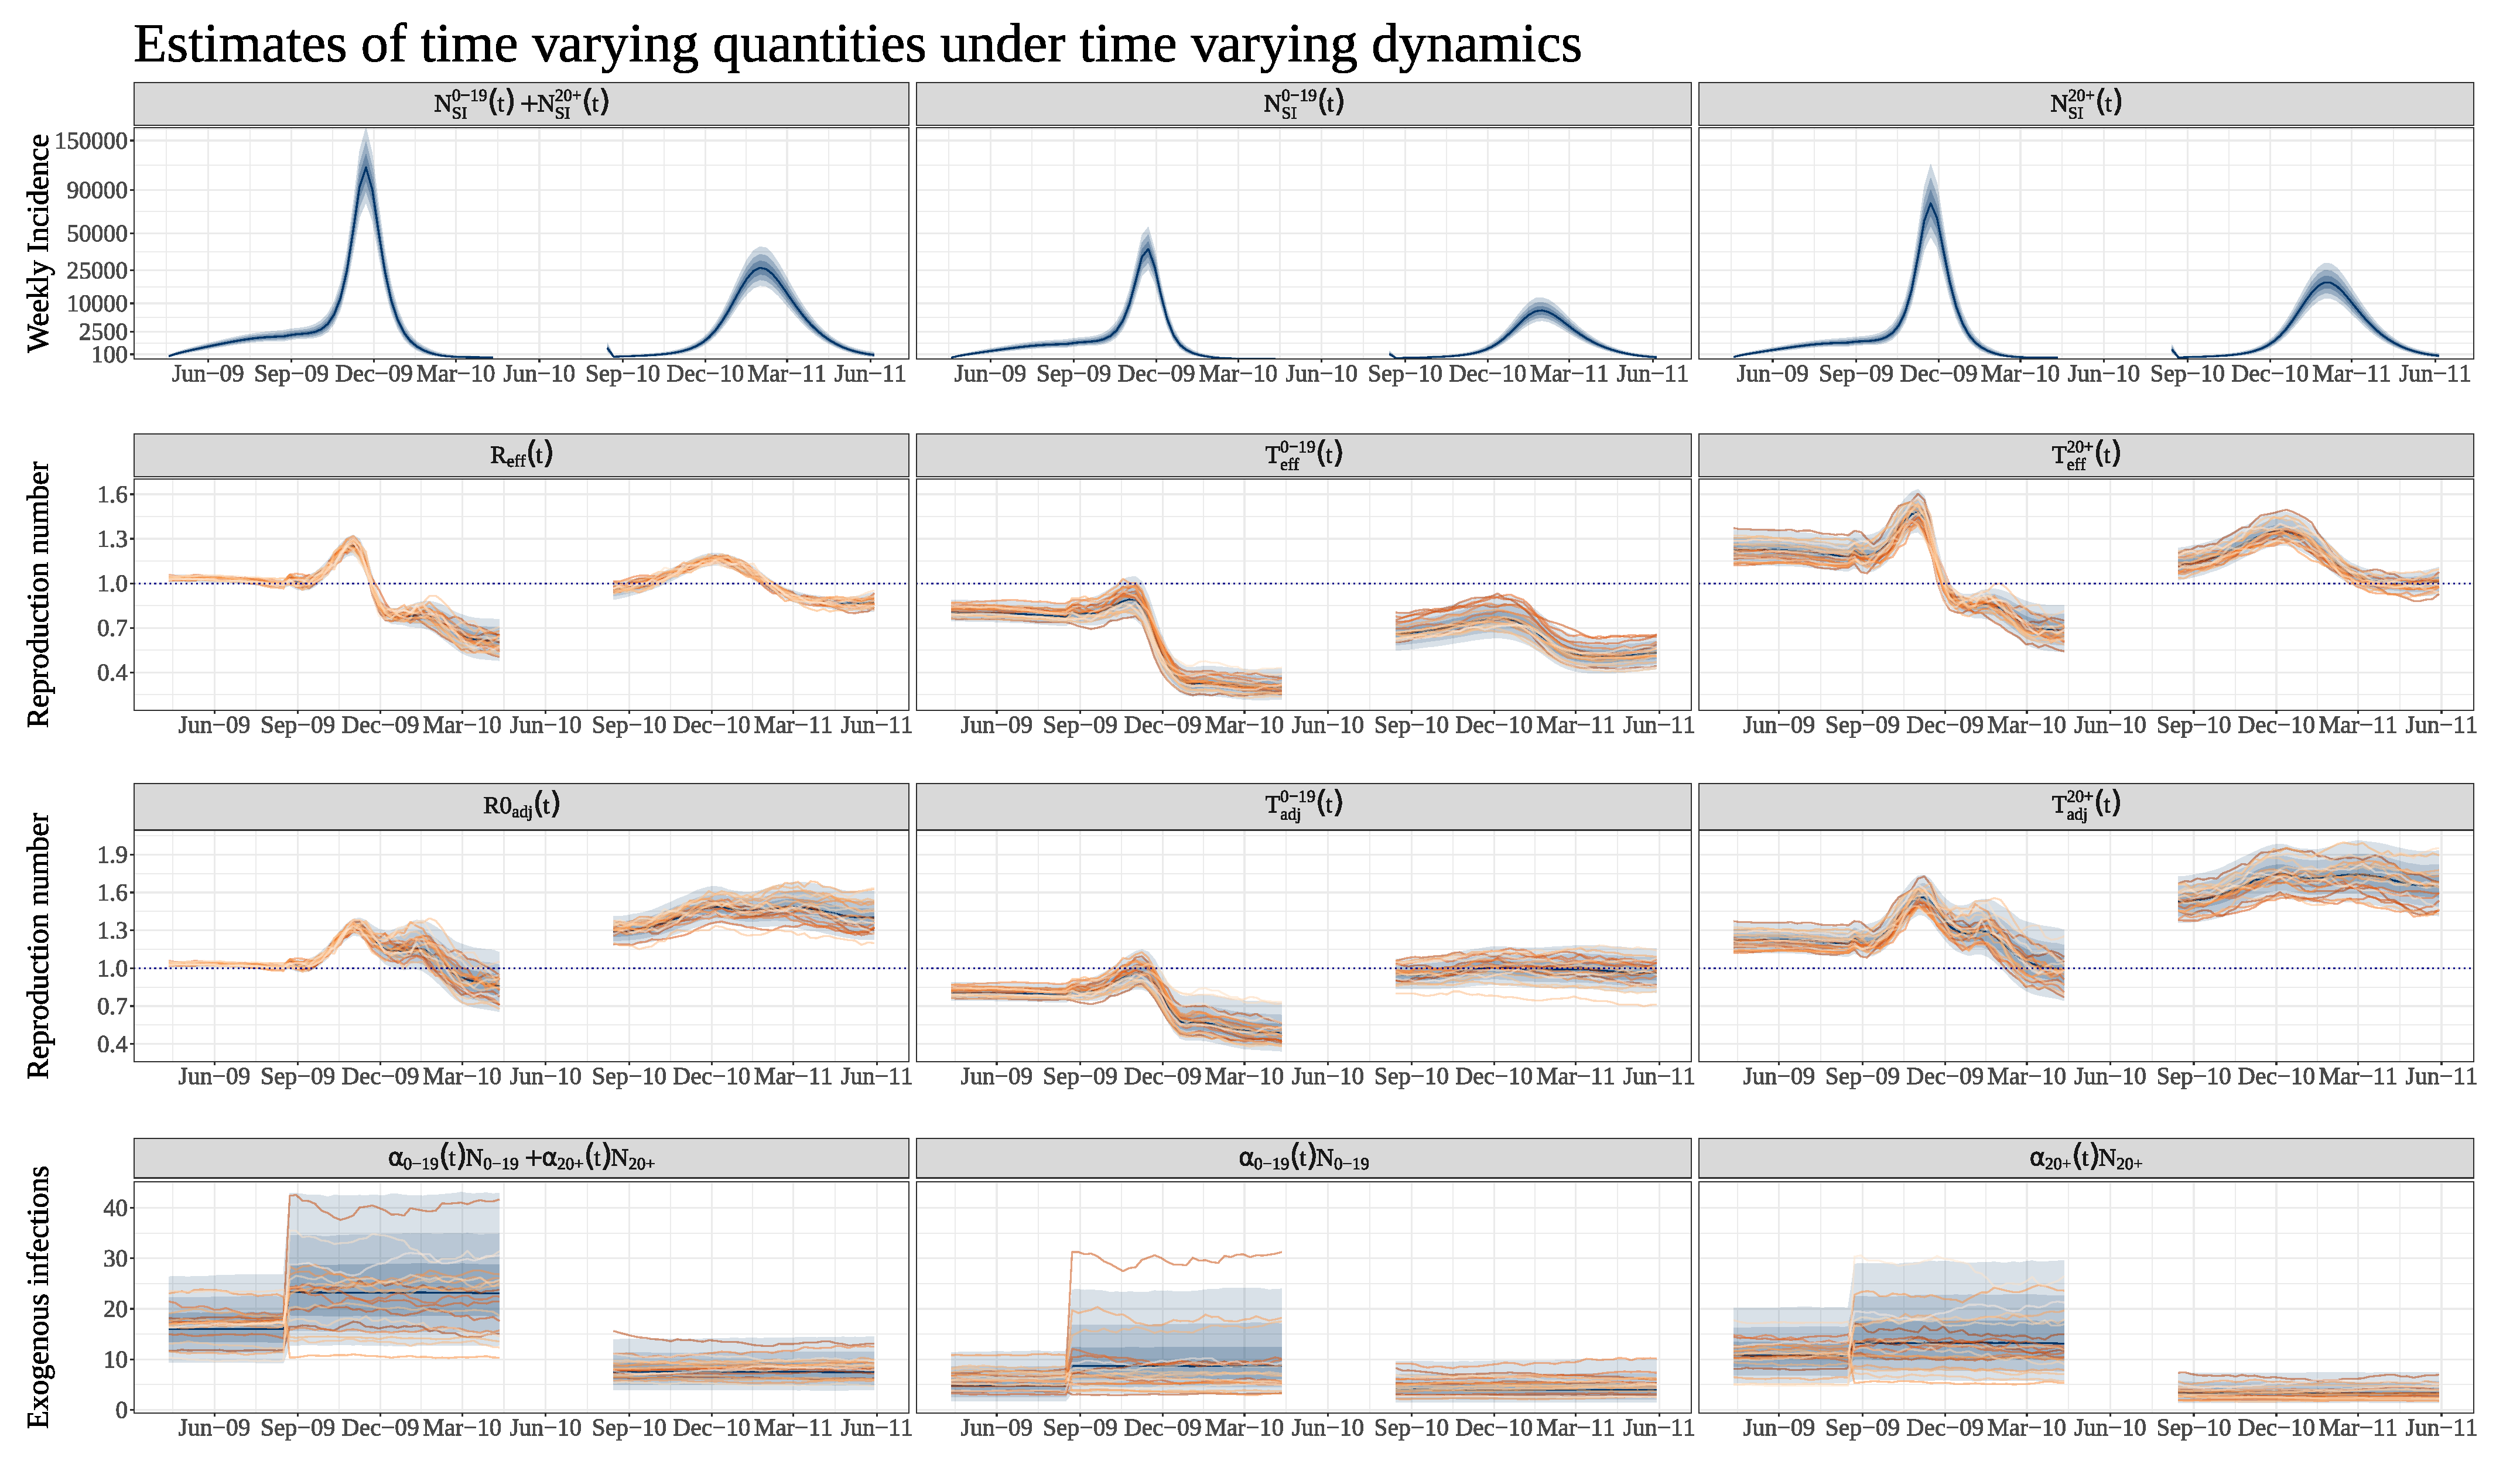
\includegraphics[width=0.95\linewidth]{figures/flu_rw_ode_timevarying_plots}
	\caption{Estimated incidence (top row), effective reproduction numbers (second row), vaccination adjusted basic reproduction numbers (third row), and exogenous infections (bottom row). $ N_{SI}^j(t), $ is the weekly incidence in age stratum $ j $, $ R_{eff}(t) $ and $ R_{adj}(t) $ are the effective and vaccination--adjusted basic reproduction numbers, $ T_{eff}^j(t) $ is the type reproduction number for stratum $ j $ (expected \# of secondary infections in all strata for a single infected in stratum $ j $), and $ \alpha_j(t) $ is the rate of exogenous infectious contacts for stratum $ j $.}
	\label{fig:flurwodetimevaryingplots}
\end{sidewaysfigure}

The mean infectious period of youths was substantially longer that of adults, 6.5 days (95\% BCI: 4.3 days, 8.8 days) compared with 2.6 days (1.9 days, 3.4 days), respectively. Published point estimates of the serial interval for A(H1N1)pdm09, which is the average time between an index case and a secondary case, and which we might expect to be a bit shorter than the mean infectious period, have mostly been in the 2--3.5 day range \cite{vink2014serial}. Immunity following infection was relatively long--lasting, although a sizable percentage of individuals who were infected lost immunity; 8.2\% (95\% BCI: 3.8\%, 16.2\%) of individuals who had become infected before the start of the second season had lost protection by the beginning of the second season, while the percentage of infected individuals who became infected over both seasons and lost it by the end of season two was 10.6\% (95\% BCI: 5.0\%, 19.9\%). 

\begin{sidewaystable}
	\caption[Posterior estimates of SIRS model parameters for pandemic A(H1N1) influenza in Finland.]{Posterior estimates of SIRS model parameters for pandemic A(H1N1) influenza in Finland. Intrinsic reproduction numbers account for vaccine coverage and vaccine efficacy via (\ref{eqn:R0t_vacc}).} 
	\label{tab:flu_param_ests}
	\centering\footnotesize
	\begin{tabular}{clrr}
		\hline
		&&\multicolumn{2}{c}{\textbf{Dynamics}}\\
		\cmidrule{3-4}\textbf{Parameter} & \textbf{Interpretation} & \textit{Time varying} & \textit{Piecewise homogeneous}\\
		\hline
		$ \psi_{Y,0} $ & Intrinsic $ R_0 $ for youths at epiweek 15, 2009  & 1.1 (1.0, 1.2) & 1.1 (1.0, 1.2)\\
		$ \psi_{Y,18} $ & Intrinsic $ R_0 $ for youths at epiweek 34, 2009 & 1.5 (1.1, 1.8) & 1.6 (1.3, 1.9)\\
		$ \psi_{Y,71} $ & Intrinsic $ R_0 $ for youths at epiweek 33, 2010 & 1.2 (0.93, 1.5) & 1.2 (0.94, 1.5)\\
		$ \psi_{A,0} $ & Intrinsic $ R_0 $ for adults at epiweek 15, 2009  & 1.1 (1, 1.2) & 1.1 (1, 1.1)\\
		$ \psi_{A,18} $ & Intrinsic $ R_0 $ for adults at epiweek 34, 2009 & 1.1 (0.95, 1.2) & 1.1 (0.96, 1.2)\\
		$ \psi_{A,71} $ & Intrinsic $ R_0 $ for adults at epiweek 33, 2010 & 1.4 (1.1, 1.8) & 1.6 (1.4, 1.8)\\
		$ 1/\mu_{Y} $ & Mean infectious period for youths (days) & 6.5 (4.3, 8.8) & 7.5 (5.5, 9.5)\\
		$ 1/\mu_A $ & Mean infectious period for adults (days) & 2.6 (1.9, 3.4) & 2.9 (2.2, 3.8)\\
		$ 1/\mu $ & Mean duration of immunity (years) & 9.3 (4.5, 21) & 9.9 (4.8, 21)\\
		$ \nu $ & 1 - VE for susceptibility & 0.05 (0.01, 0.17) & 0.04 (0.01, 0.13)\\
		$ \rho_Y $ & Mean case detection rate for youths & 0.008 (0.006, 0.012) & 0.008 (0.006, 0.011)\\
		$ \rho_A $ & Mean case detection rate for adults & 0.003 (0.002, 0.005) & 0.003 (0.002, 0.004)\\		
		$ 1/\sqrt{\phi_Y} $ & Negative binomial overdispersion for youths & 0.99 (0.82, 1.2) & 1 (0.85, 1.3)\\
		$ 1/\sqrt{\phi_A} $ & Negative binomial overdispersion for adults & 0.97 (0.83, 1.2) & 1 (0.83, 1.2)\\
		\hline
	\end{tabular}
\end{sidewaystable}

\subsection{Piecewise Homogeneous Dynamics}
\label{subsec:flu_res_homog}

\section{Discussion}
\label{sec:flu_discussion} % pandemic influenza analysis
\chapter{Discussion and Future Work} % discussion and future work

\printendnotes

%
% ==========   Bibliography
%
\nocite{*}   % include everything in the uwthesis.bib file
\bibliographystyle{plain}
\bibliography{fintzi_dissertation}
%
% ==========   Appendices
%
\appendix
\raggedbottom\sloppy
\chapter{Appendix to Chapter 4}
\label{chap:appendix_ch4}

\section{Tuning the Initial Elliptical Slice Sampling Bracket Width}
\label{sec:lna_init_bracket_width}

When fitting SEMs with complex dynamics, e.g., when there are many strata or when the dynamics are time varying, we will be able improve the computational efficiency of our MCMC by initialing the ElliptSS bracket width at $ \omega < 2\pi $. This choice is motivated by the observation that when the model dynamics are complex, the ElliptSS bracket will typically need to be shrunk many times before the sampler reaches a range of acceptable angles in the proposal. Each time we propose a new angle in the ElliptSS algorithm we must solve the LNA ODEs in order to compute the observed data likelihood. Thus, if we can reduce the number of ElliptSS steps, we will be able to shorten the time required to complete our MCMC runs. 

In models where it is advantageous to shring the initial bracket width, we will typically set the initial bracket width to a constant times the standard deviation of the accepted angles in a tuning phase. Since we do not step out the ElliptSS bracket, the initial width should not be so small as to induce additional autocorrelation in the latent process, and should also not be so wide that the bracket is contracted needlessly. We have found a bracket width of $ \omega = 2\sqrt{2\log(10)}\sigma $, corresponding to the full width at one tenth maximum for a Gaussian with standard deviation $ \sigma $, to work well in practice. Figure \ref{fig:esstuning} presents histograms of the number of contractions per ElliptSS update and the accepted angles before and after contracting the initial ElliptSS bracket width for the joint Ebola model of Section \ref{sec:lna_ebola}. In this instance, we were able to substantially reduce the number of contractions, and hence likelihood evaluations, per ElliptSS update while leaving the distribution of accepted angles essentially unchanged. We like to call this a "free lunch".

\begin{figure}
	\centering
	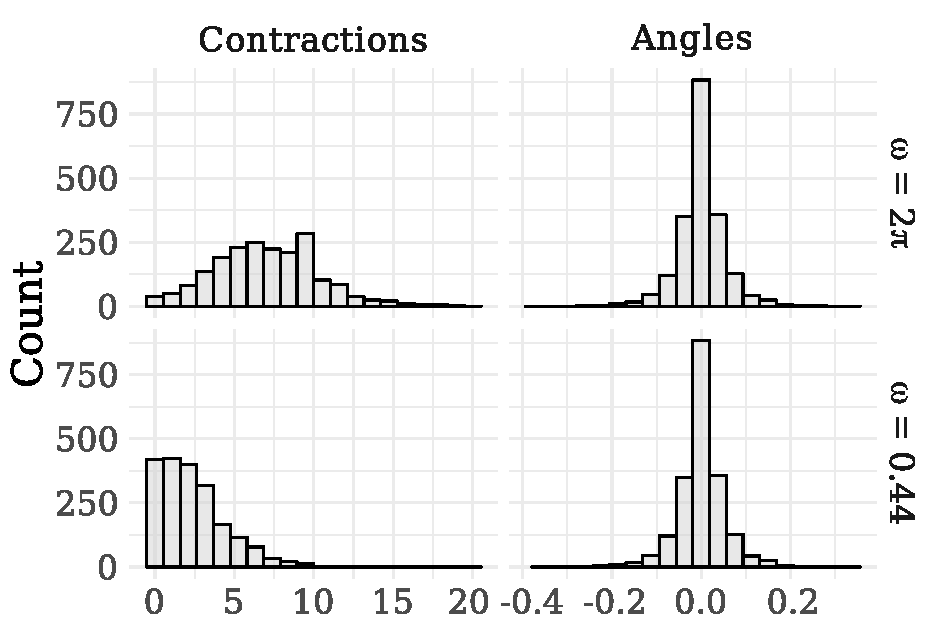
\includegraphics[width=0.7\linewidth]{figures/ess_tuning}
	\caption[Distributions of numbers of contractions and accepted for elliptical slice sampling.]{Distributions of the numbers of contractions per ElliptSS update and the accepted angles for an MCMC chain for the joint Ebola model of Section \ref{sec:lna_ebola} . An initial bracket width of $ 2\pi $ was used for the first 5,000 iterations (top row), after which the initial bracket width was set to $ 2\sqrt{2\log(10)}\sigma_{ElliptSS} $, where $ \sigma_{ElliptSS} $ was the standard deviation of the accepted angles from the initial run (bottom row).} 
	\label{fig:esstuning}
\end{figure}

We mentioned in Section \ref{subsubsec:noncentered_parameterization} that our ElliptSS algorithm was modified slightly from that presented in \cite{murray2010} in order to facilitate tuning of the initial ElliptSS bracket width. In both cases, the distribution of proposed states, $ \bZ_{prop} $, is centered at the current state $ \bZ_{cur} $. However, the distribution of angles of accepted states using our algorithm will be centered around 0, whereas the distribution of angles for accepted proposals using the algorithm in \cite{murray2010} will be bimodal with peaks at 0 and $ 2\pi $. The algorithms are nevertheless equivalent due to the rotational symmetry of the proposals (a proposal made using an angle $ \phi $ is equivalent to a proposal using $ \phi+2\pi $). It is more natural to compute the standard deviation of the accepted angles if the distribution of angles is symmetric about zero than if it is bimodal (and would thus require a rotation).

\section{Inference for Initial Compartment Volumes}
\label{sec:lna_init_volumes}

When the initial compartment volumes are included as initial parameters in the model instead of being treated as fixed, we will model them as arising from the following truncated multivariate normal distribution: \begin{equation}
\label{eqn:lna_initdist_prior}
\bX_0 \sim TMVN_{\mcS_X^R}(N\bp,N(\bP - \bp\bp^T)),
\end{equation} 
where $ \bp $ is a vector of subject--level initial state probabilities, $ \bP = \diag(\bp) $, $ N $ is the population size, and the subscript $ \mcS_X^R $ specifies the state space of $ \bX $ (so that the compartment volumes add up to $ N $ and each compartment volume is non--negative and less than the total population size at time $ t_0 $). Thus, the initial distribution is specified as the truncated normal approximation of a multinomial distribution with size $ N $ and probability vector $ \bp $. In models with multiple strata, we will similarly model the initial compartment volumes as having independent truncated multivariate normal distributions that are each approximations of multinomial distributions over initial compartment counts within each stratum. Notation and details are completely analogous to the single stratum case, and are therefore omitted for the sake of clarity.

Let $ \bV = N(\bP - \bp\bp^T) $, and $ \bV^{1/2} $ be the matrix square root of $ \bV $, which we will compute using the singular value decomposition $ \bV = \bU\bD\bU^T \implies \bV^{1/2} = \bU\bD^{1/2}$. Let $ \bZ^X $ denote the LNA draws as before, and let $ \bZ^{X_0}\sim\mr{MVN}(\bs{0},\mb{I}) $ denote the vector of draws that will be mapped to $ \bX_0 $. We will update the initial compartment volumes jointly with the LNA draws using elliptical slice sampling.

\begin{algorithm}[htbp]
	\caption{Sampling LNA draws and initial volumes via elliptical slice sampling.}
	\label{alg:elliptss_lna_initvols}
	\begin{algorithmic}[1]
		\Procedure{\doElliptSS2}{$ \bZ^X_{cur}, \bZ^{X_0}_{cur},\btheta,\bY,\mcI,\omega = 2\pi $}
		\State Sample ellipse: $ \bZ^X_{prop} \sim N(\bs{0}, \mb{I}),\ \bZ^{X_0}_{prop} \sim N(\bs{0}, \mb{I})$
		\State Sample threshold: $ u|\bx \sim \mr{Unif}(0, L(\bY|\doLNA(\bZ_{cur},\btheta,\mcI))) $
		\State Position the bracket and make initial proposal: \vspace{-0.1in}
		\begin{align*}
		\psi &\sim \mr{Unif}(0,\omega)\\
		L_\psi &\leftarrow -\psi;\ R_\psi \leftarrow L_\psi + \psi\\
		\phi &\sim \mr{Unif}(L_\psi,R_\psi)
		\end{align*}
		\State Set $ \bZ^{X'} \leftarrow \bZ^X_{cur}\cos(\phi) + \bZ^X_{prop}\sin(\phi) $, $ \bX_0^\prime = \bV^{1/2}\left (\bZ^{X_0}_{cur}\cos(\phi) + \bZ^{X_0}_{prop}\sin(\phi)\right ) $ 
		\If{$ L(\bY|\doLNA(\bZ',\btheta^\prime,\mcI)) > u $}{ accept $ \bZ^{X^\prime},\bZ^{X_0^\prime} $}
		\State\Return{ $ \bZ' $}
		\Else
		\State Shrink bracket and try a new angle:
		\State{\textbf{If:} $ \phi < 0 $}{ \textbf{then: }$ L_\phi \leftarrow\phi $ }{ \textbf{else: }$ R_\phi \leftarrow \phi $}
		\State $ \phi \sim \mr{Unif}(L_\phi, R_\phi) $
		\State \textbf{GoTo:} 5
		\EndIf
		\EndProcedure
	\end{algorithmic}
\end{algorithm}

\section{Choice of Estimation Scale and Implications for Mixing and Convergence}
\label{sec:est_scale_discussion}

How we parameterize the MCMC estimation scale is critically important to its computational performance. If we can identify transformations of the model parameters that minimize strong correlations and non--linear relationships on the estimation scale, we will be able to substantially improve MCMC mixing. In our context, it will often be relatively straightforward to identify such transformations (or at least intermediate transformations that can be used in combination). As a general approach, we will try to identify transformations that reflect the ways in which model parameters jointly act on the model dynamics, and then a second set of transformations that remove any boundary conditions. 
\begin{table}[htbp]
	\caption{SEIR model parameter and their interpretation on their natural scales.}
	\label{tab:seir_params_nat}
	\footnotesize
	\centering
	\begin{tabular}{clc}
		\hline
		\textbf{Parameter} & \textbf{Interpretation} & \textbf{Domain}\\
		\hline
		$\alpha$ & Rate of infectious contact from outside the population & $[ 0,\infty) $ \\
		$ \beta $ & Per--contact rate of infection within the population & $[0,\infty) $\\
		$ \omega $ & Rate of transition from $ E\rightarrow I $ & $[ 0,\infty) $\\
		$ \mu $ & Rate of transition from $ I\rightarrow R $ & $[ 0,\infty) $\\
		$ \rho $ & Mean case detection probability & $[ 0,1] $\\
		$ \phi $ & Negative binomial overdispersion parameter & $[ 0,\infty) $ \\
		$ N_{eff} $ & Effective population size & $[0,N]$\\
		\hline
	\end{tabular}
\end{table}

As an example, consider the single country SEIR model fit to the incidence data from Sierra Leone in Section \ref{sec:lna_ebola}. This model includes parameters for the external force of infection and the effective population size, which add complexity to the usual formulation of the SEIR dynamics as being entirely driven by endogenous contacts within a closed homogeneously mixing population. The model parameters on their natural scales are provided in Table \ref{tab:seir_params_nat}. Each of the model parameters has a clear marginal interpretation, but upon examining the pairwise scatterplots of the posterior (Figure \ref{fig:slpairs1}) it becomes obvious that the parameters interact in highly non--linear ways. We would encounter a variety of pathological computational problems if we were to naively parameterize the MCMC estimation scale without considering the ways in which the parameters interact to affect the dynamics. For example, it would be extremely difficult for any sampler that does not account for the curvature in the posterior, e.g., Hamiltonian Monte Carlo (HMC), to explore the parameter space. (An aside: we experimented with implementing the LNA in \texttt{Stan} and using HMC to sample the posterior, but repeatedly integrating the LNA ODEs along with their augmented sensitivity equations was prohibitively slow for even simple models).  

\begin{figure}[htbp]
	\centering
	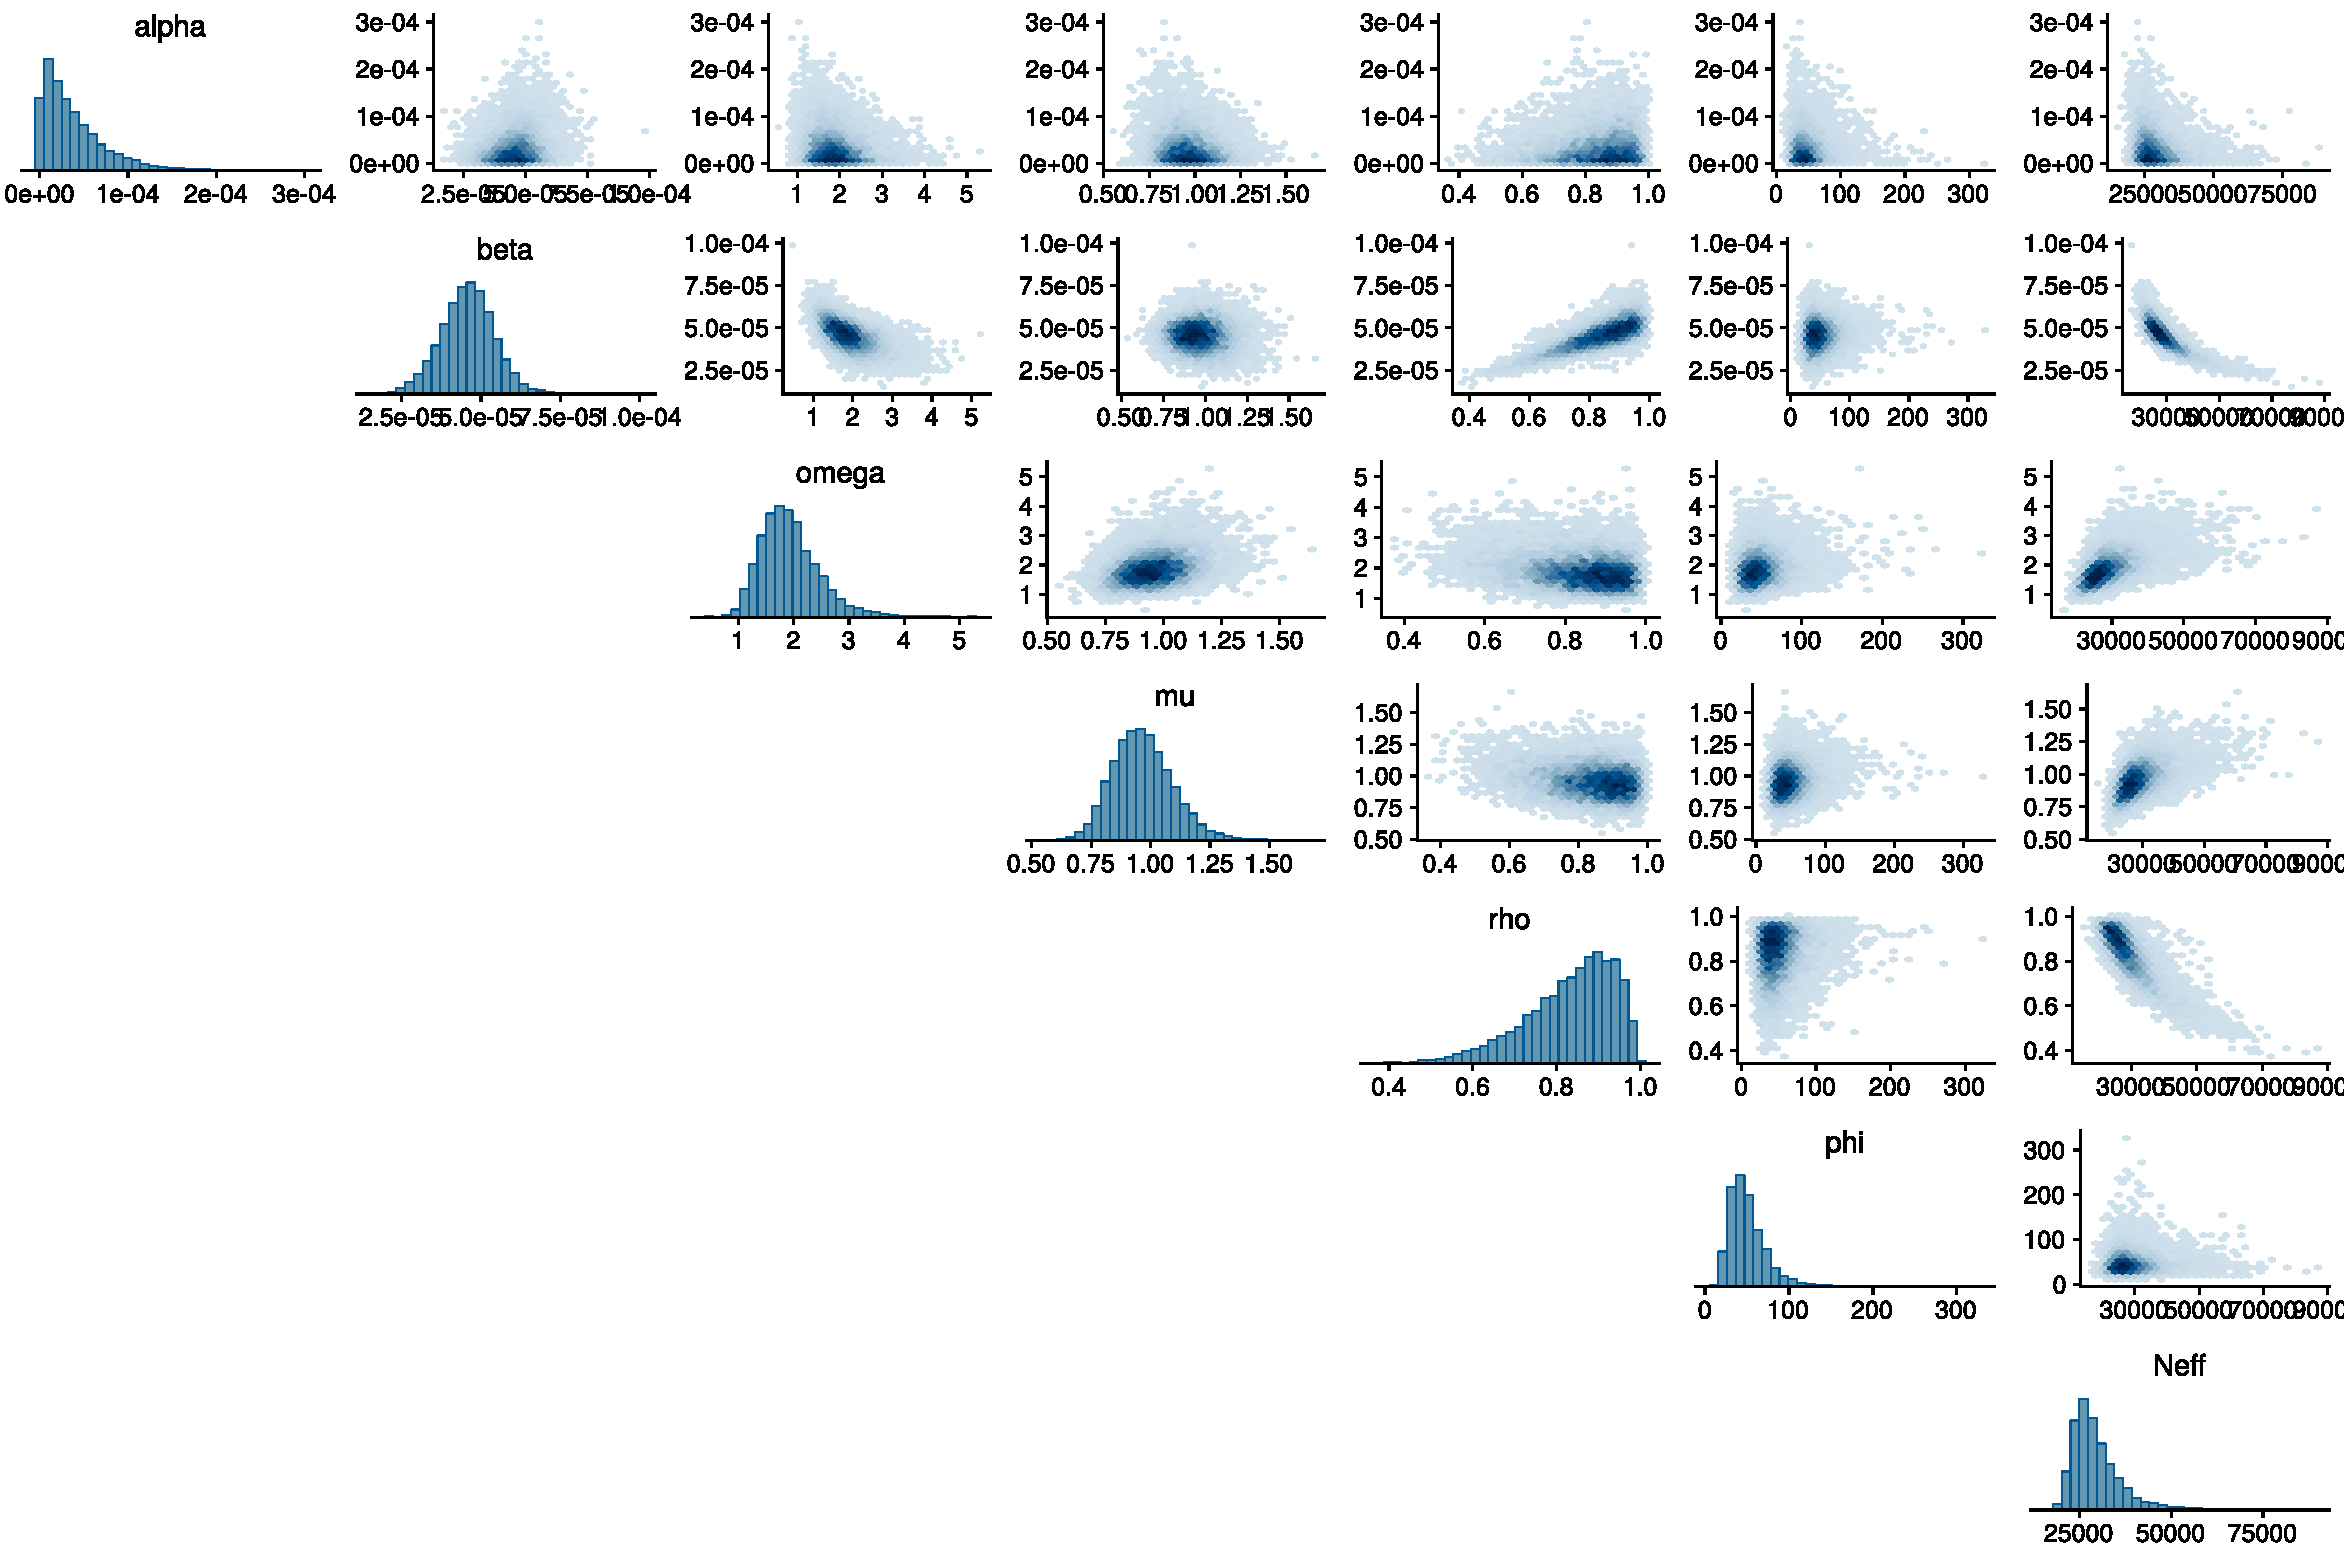
\includegraphics[width=\linewidth]{figures/sln_pairs_nat}
	\caption[Posterior scatterplots for Sierra Leone SEIR model parameters on their natural scales.]{Marginal histograms and pairwise scatterplots of posterior samples for parameters for the SEIR model fit to the Sierra Leone Ebola dataset using the estimation scale in Table \ref{tab:seir_params_est3}. The parameters on the estimation scales in this figure and their interpretations are provided in Table \ref{tab:seir_params_nat}.} 
	\label{fig:slpairs1}
\end{figure}

We can mitigate the problems caused by non--linear relationships and strong correlations among parameters by parameterizing the estimation scale in terms of how the parameters jointly affect the model dynamics and then removing the boundary conditions. Table \ref{tab:seir_params_est2} provides a list of parameters on their estimation scale that are reflective of an initial first pass at how we would expect the parameters to interact. For example, the parameters governing the rates of infectious contact, $ \alpha$ and $\beta $, combine with the effective population size and the infectious period duration to produce the basic reproductive numbers with respect to initially infected individuals outside and inside the population. Still, we can see that there are some residual non--linear relationships between the log effective population size, the logit case detection probability, and the effective reproductive number.

\begin{table}[htbp]
	\caption{SEIR model parameter and their interpretation on a possible set of estimation scales.}
	\label{tab:seir_params_est2}
	\footnotesize
	\centering
	\begin{tabular}{clc}
		\hline
		\textbf{Parameter} & \textbf{Interpretation} & \textbf{Domain}\\
		\hline
		$\log(R_{eff}^{ext}) = \log(\alpha N_{eff} / \mu)$ & \makecell[l]{Log basic reproductive number given an infected \\outside the population} & $(-\infty,\infty) $ \\
		$ \log(R_{eff} - 1) = \log(\beta N_{eff}/\mu - 1) $ & \makecell[l]{Log basic reproductive number given an infected\\ inside the population and $ R_{eff} > 1 $.} & $(-\infty,\infty) $\\
		$ \log(1/\omega) $ & Log mean latent period duration & $(-\infty,\infty) $\\
		$ \log(1/\mu) $ & Log mean infectious period duration & $ (-\infty,\infty) $\\
		$ \logit(\rho) $ & Logit mean case detection probability & $(-\infty,\infty) $\\
		$ \log(\phi) $ & Log negative binomial overdispersion parameter & $ (-\infty,\infty) $ \\
		$ \log(N_{eff}) $ & Log effective population size & $(-\infty,\log(N))$\\
		\hline
	\end{tabular}
\end{table}

\begin{figure}[htbp]
	\centering
	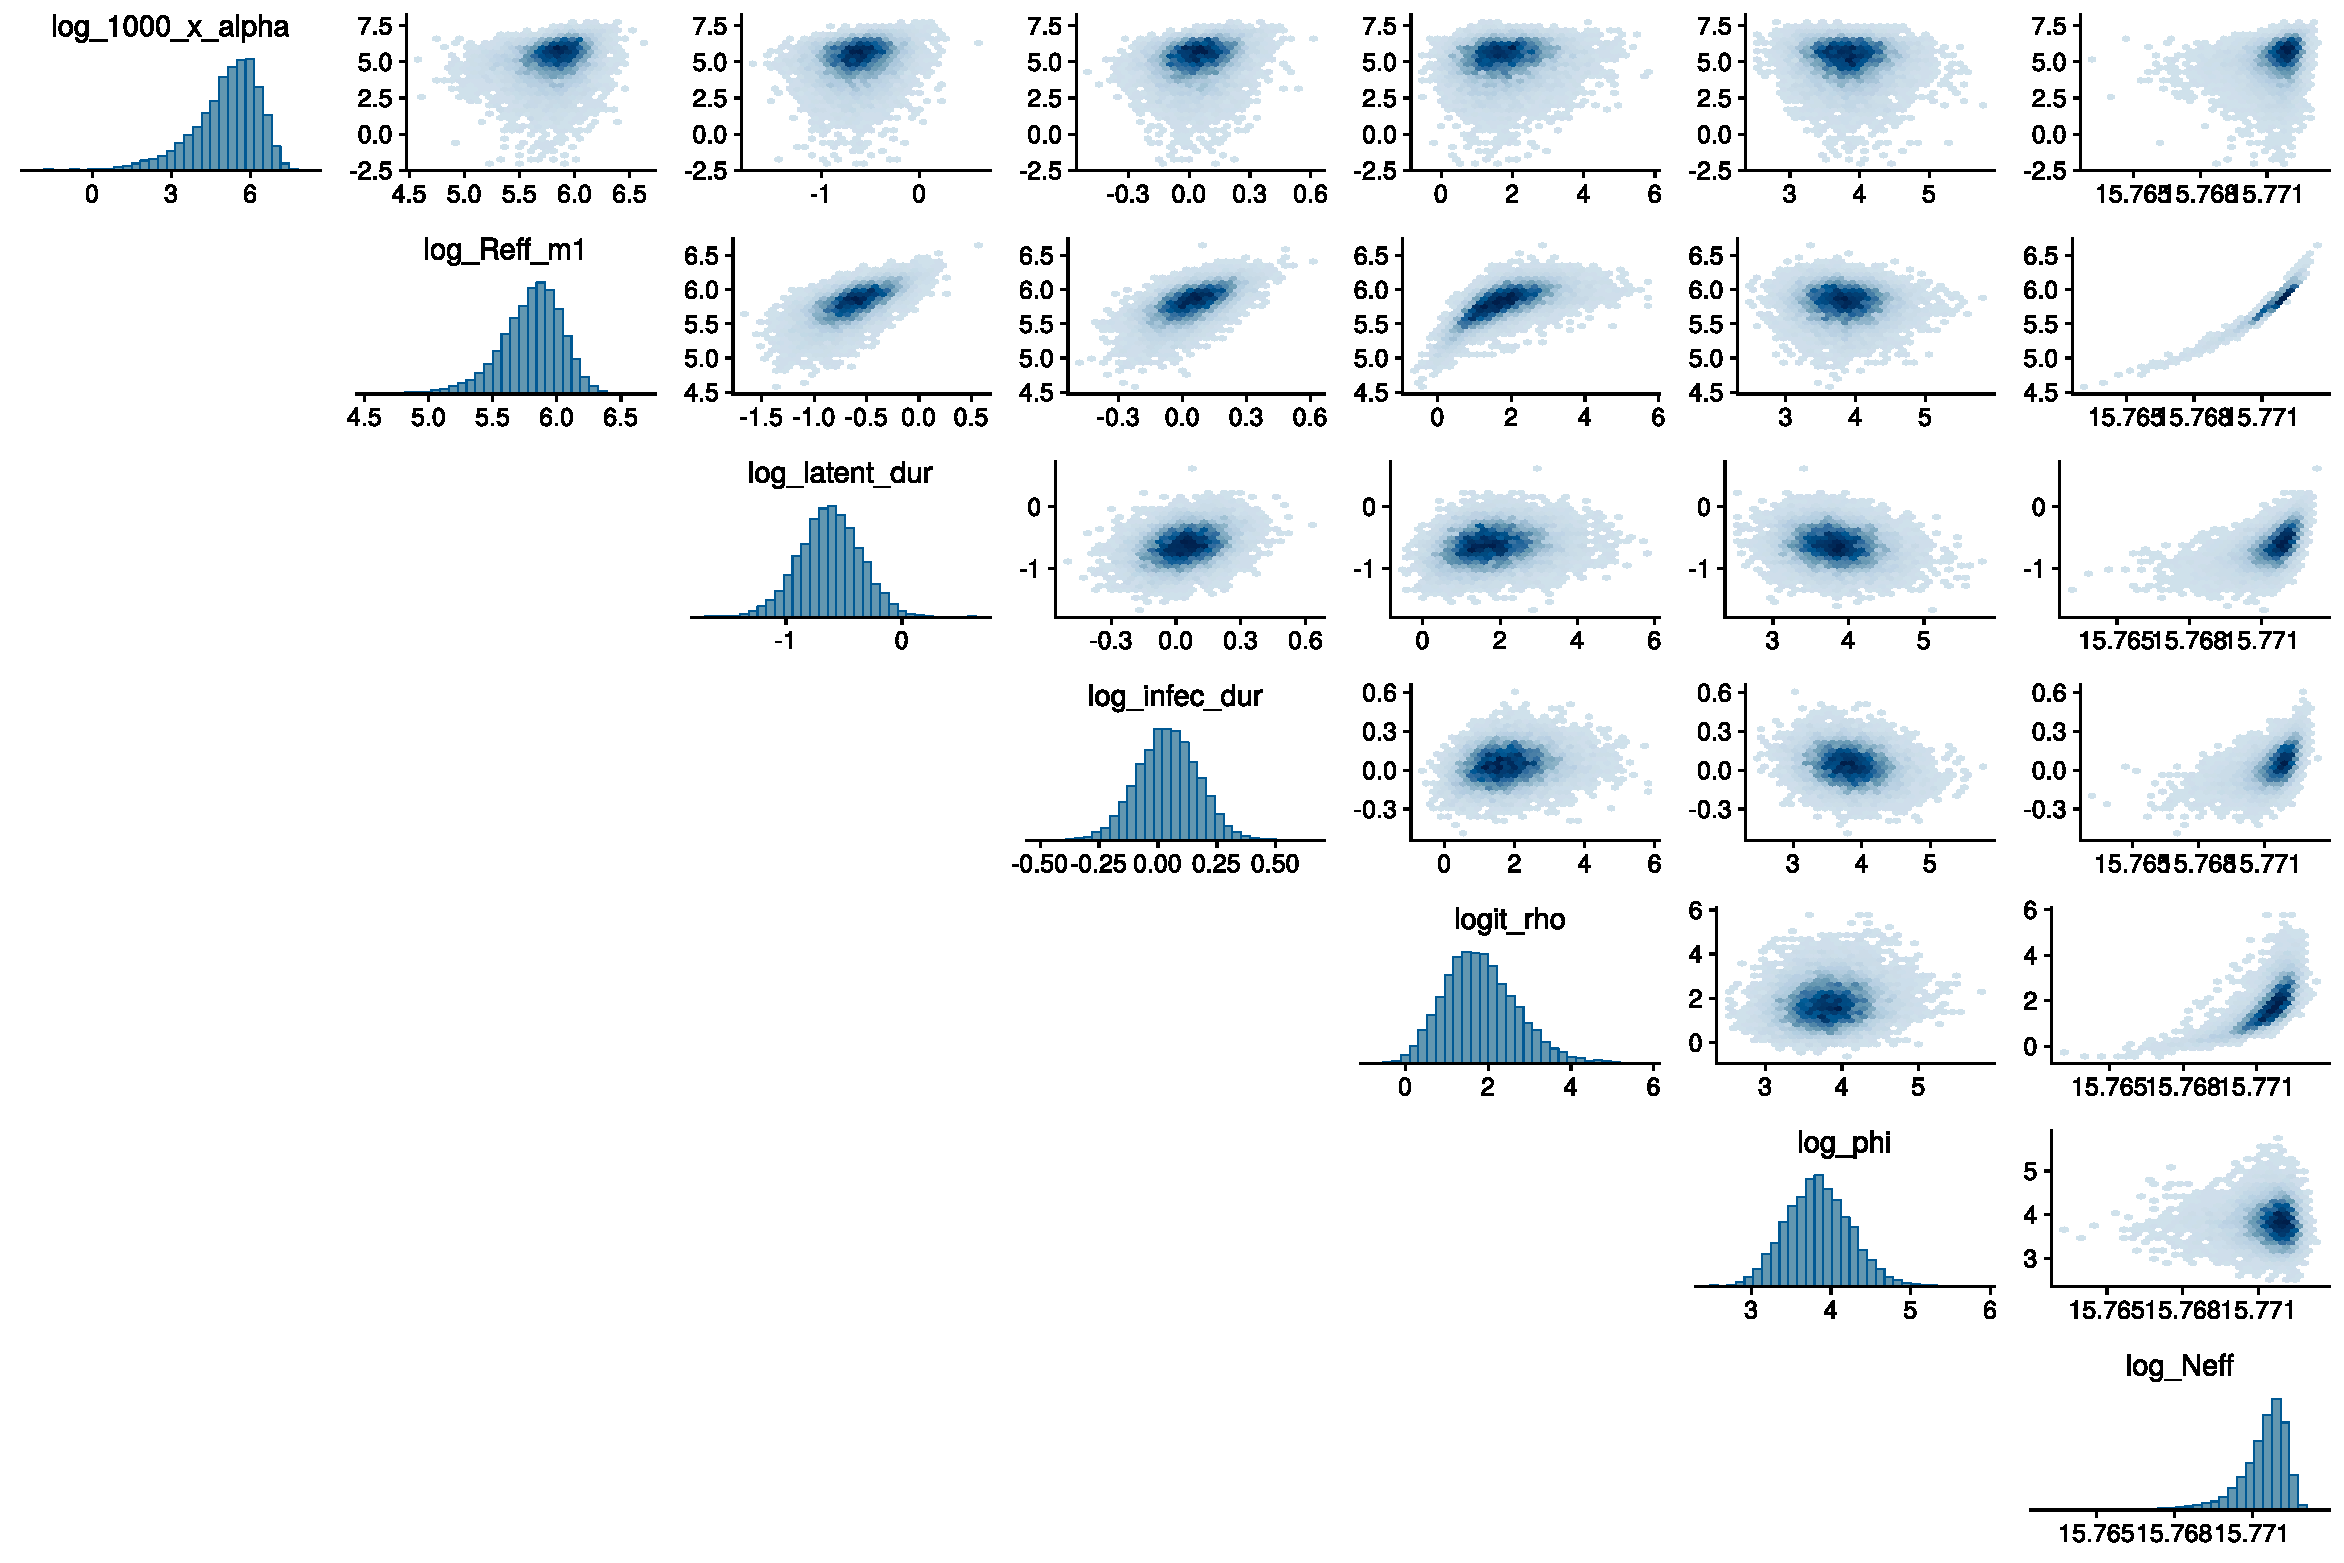
\includegraphics[width=\linewidth]{figures/sln_pairs_t1}
	\caption[Posterior scatterplots for transformed Sierra Leone SEIR model parameters.]{Marginal histograms and pairwise scatterplots of posterior samples for parameters for the SEIR model fit to the Sierra Leone Ebola dataset using the estimation scale in Table \ref{tab:seir_params_est3}. The parameters on the estimation scales in this figure and their interpretations are provided in Table \ref{tab:seir_params_est2}.} 
	\label{fig:slpairs2}
\end{figure}

We should give additional consideration to how the previous functions of model parameters interact within the model. The effective population size, on its own, in this model is essentially a nuisance parameter. However, combined with the mean case detection probability, the mean case detection rate, $ \rho N_{eff} $ should be, more or less, on the same scale as the total number of observed cases modulo the fraction of the effective population to escape infection. We note that estimation of this quantity is stable even when the population size is misspecified, see, e.g., \cite{fintzi2017efficient, koepke2016predictive}. Moreover, we should suspect, \textit{a priori}, that the basic reproductive number interacts with the mean case detection rate. To understand this, we examine how the basic reproductive number acts on the outbreak size through the final size relation for the deterministic ODE analog to our model \cite{bauer2008compartmental}: 
\begin{equation}
\label{eqn:final_size_relation}
\log\frac{S_0}{S_\infty} = R0\left (1 - \frac{S_\infty}{N}\right ).
\end{equation}
This equation relates the fraction of the population that eventually becomes infected with the basic reproductive number. As $ R0 $ increases, a larger fraction of the population becomes infected. If the effective population size is large, and if the $ R0 $ is high, the mean case detection probability should be low so that the mean case detection rate is concordant with the scale of the observed counts. This is all to suggest that the combination of parameters that jointly acts on the model is the effective reproductive number, offset by the mean case detection rate. The other reparameterization we suggest is to use the infectious period duration and the ratio of the latent to infectious period durations. The new estimation scale is given in Table \ref{tab:seir_params_est3}. On this estimation scale, the posterior for Sierra Leone is much better behaved, with weaker pairwise correlations and very little in the way of non--linear relationships between the model parameters.

\begin{table}[htbp]
	\caption{SEIR model parameter and their interpretation on a possible set of estimation scales.}
	\label{tab:seir_params_est3}
	\footnotesize
	\centering
	\begin{tabular}{clc}
		\hline
		\textbf{Parameter} & \textbf{Interpretation} & \textbf{Domain}\\
		\hline
		$\log(1000\alpha)$ & \makecell[l]{Log effective number of additional infecteds per \\ 1000 infecteds outside the population} & $(-\infty,\infty) $ \\
		$ \log(R_{eff} - 1) + \log(\rho N_{eff}) $ & \makecell[l]{Log basic reproductive number given an infected\\ inside the population and $ R_{eff} > 1 $, offset\\ by the mean case detection rate} & $(-\infty,\infty) $\\
		$ \log(\omega/\mu) $ & Log ratio of mean latent to infectious period durations & $(-\infty,\infty) $\\
		$ \log(1/\mu) $ & Log mean infectious period duration & $ (-\infty,\infty) $\\
		$ \logit(\rho) $ & Logit mean case detection probability & $(-\infty,\infty) $\\
		$ \log(\phi) $ & Log negative binomial overdispersion parameter & $ (-\infty,\infty) $ \\
		$ \log(\rho N_{eff}) $ & Log mean case detection rate & $(-\infty,\log(N))$\\
		\hline
	\end{tabular}
\end{table}

\begin{figure}[htbp]
	\centering
	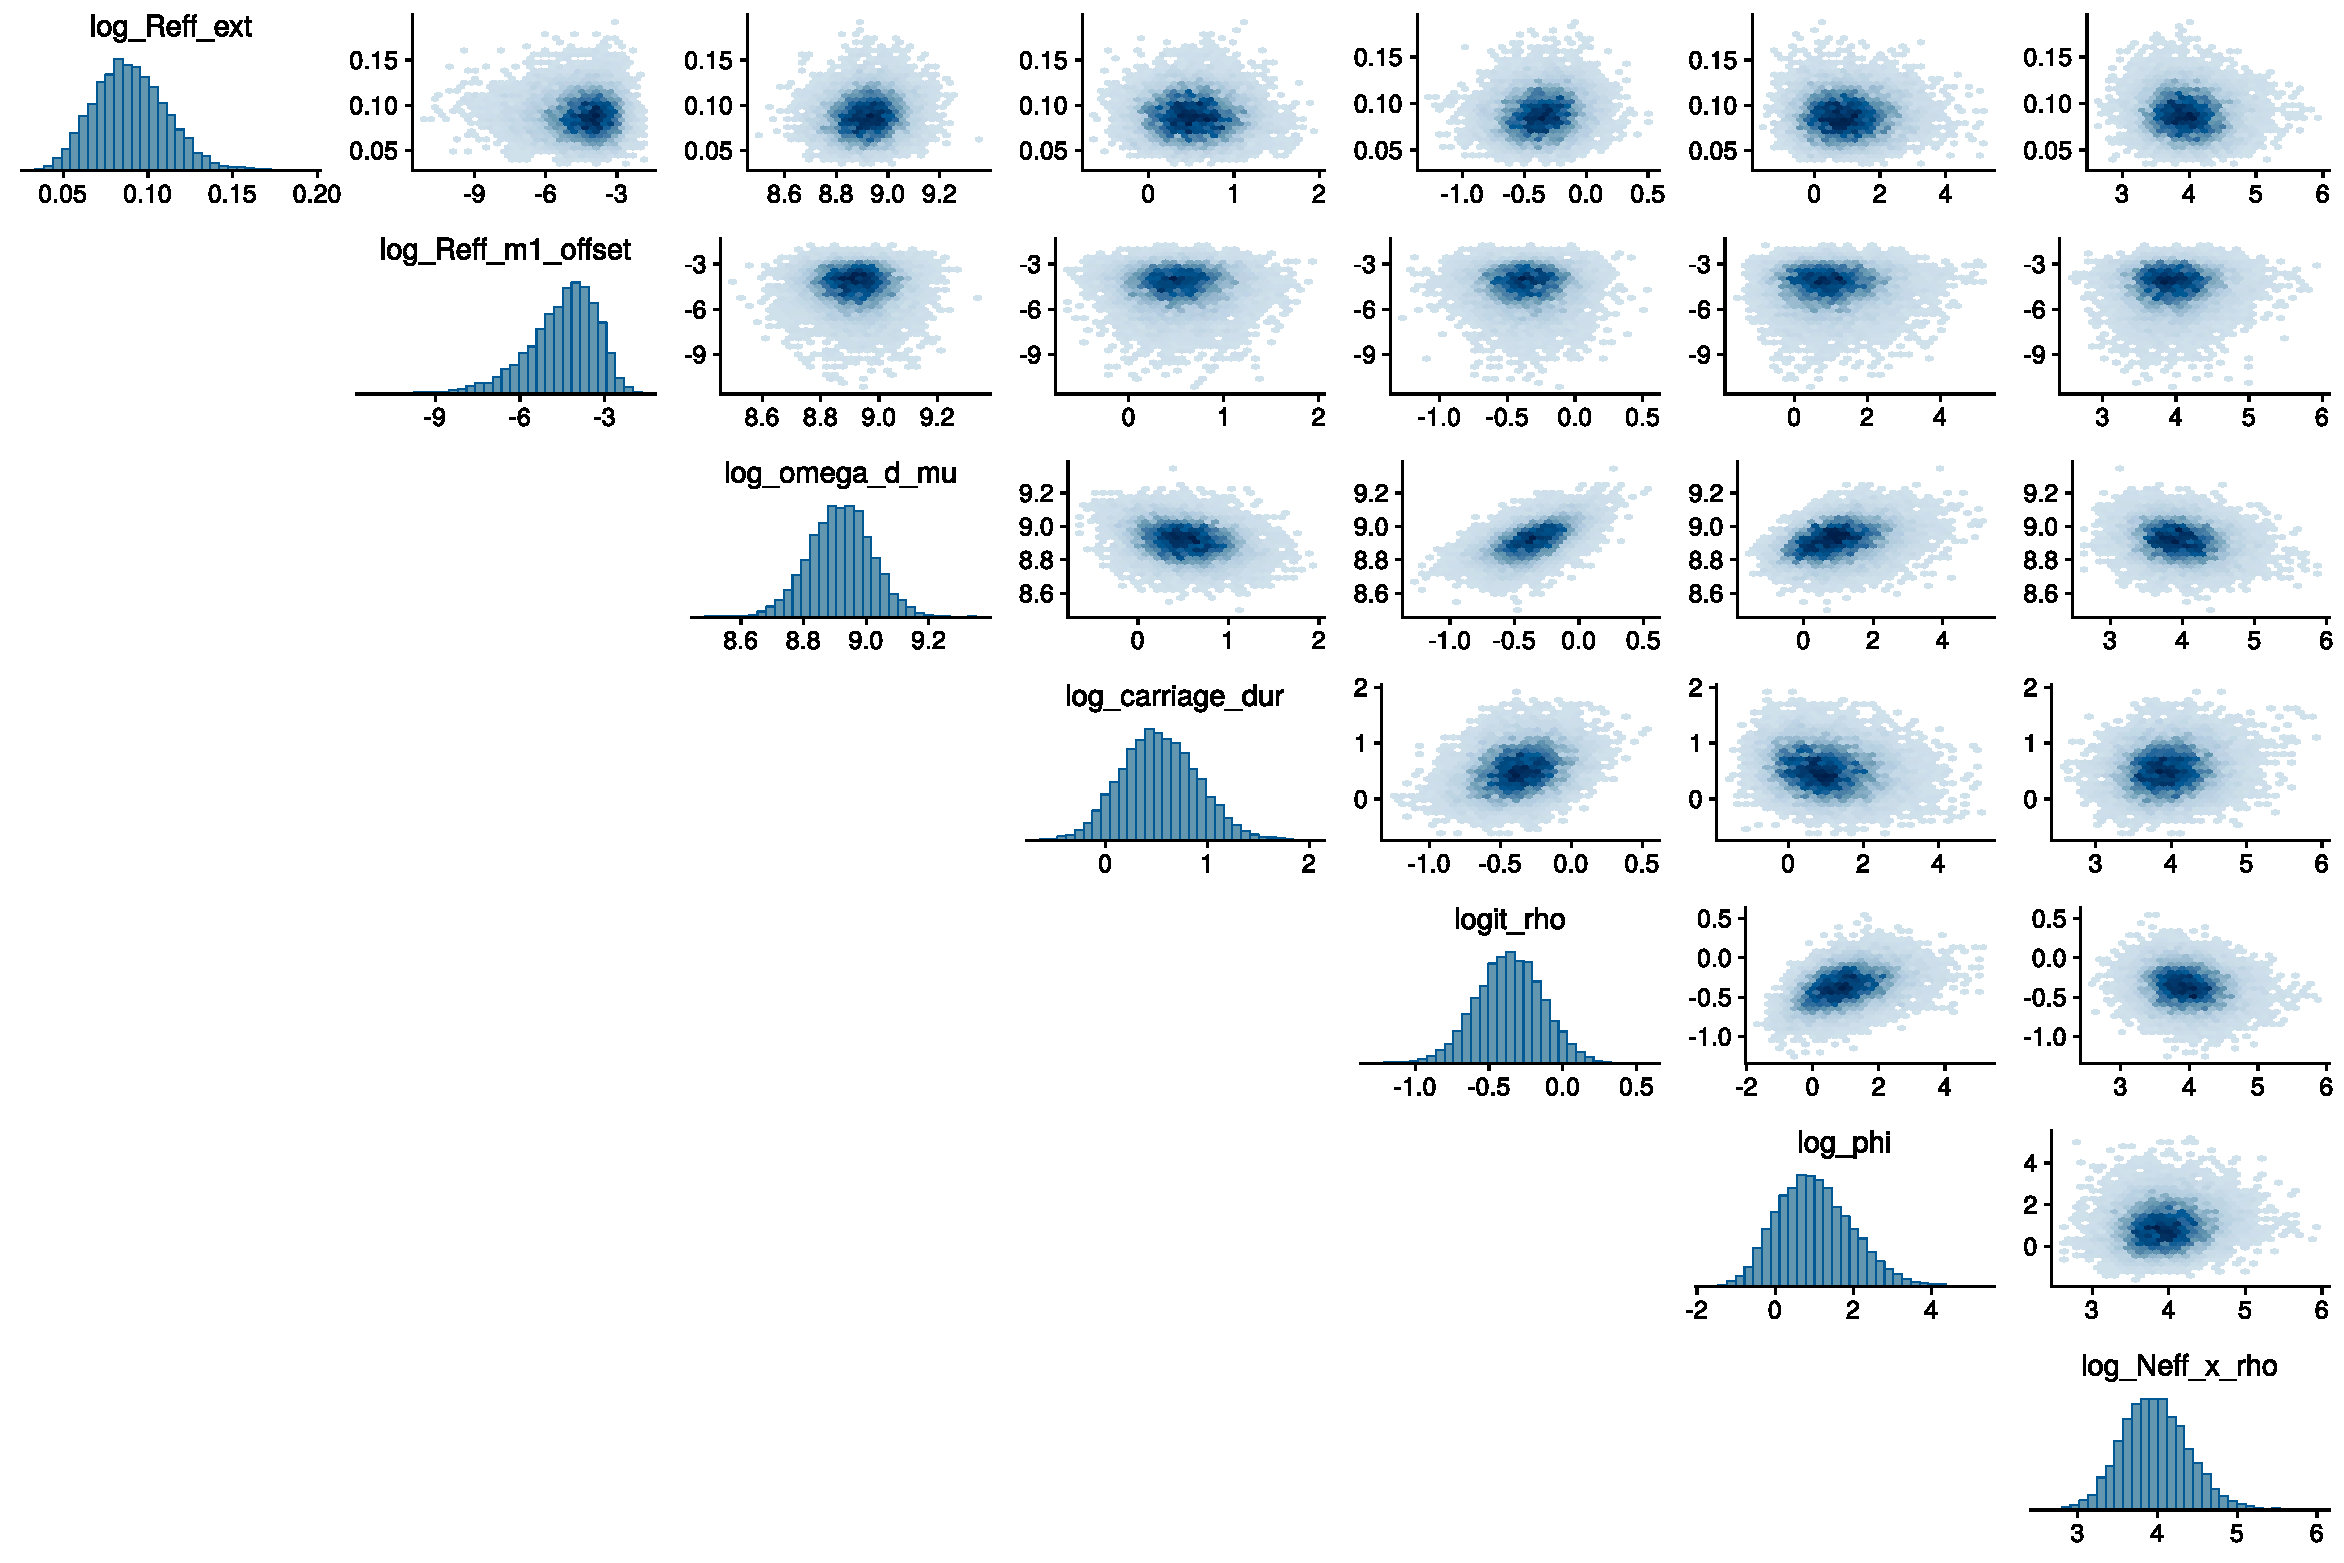
\includegraphics[width=\linewidth]{figures/sln_pairs_t2}
	\caption[Posterior scatterplots for linear combinations of transformed Sierra Leone SEIR model parameters.]{Marginal histograms and pairwise scatterplots of posterior samples for parameters for the SEIR model fit to the Sierra Leone Ebola dataset using the estimation scale in Table \ref{tab:seir_params_est3}. The parameters on the estimation scales in this figure and their interpretations are provided in Table \ref{tab:seir_params_est3}.} 
	\label{fig:slpairs3}
\end{figure}

\newpage
\section{Simulation Details and Additional Results for Section \ref{subsec:lna_coverage}}
\label{sec:lna_coverage_supplement}

\subsection{Simulation Setup and MCMC Details}
\label{subsec:lna_coverage_setup_details}

In this simulation, repeated for each of the three different regimes of population size and initial conditions given in Table \ref{tab:lna_coverage_sim}, we simulated 500 datasets according to the following procedure:
\begin{enumerate}
	\item Draw $ \log(R0 - 1),\ 1/\mu,\ \logit(\rho),\ \log(\phi) $ from the priors given in Table \ref{tab:lna_coverage_sim}.
	\item Simulate an outbreak, $ \bN|\btheta $, under SIR dynamics from the MJP via Gillespie's direct algorithm \cite{gillespie1976general}. If there were fewer than 15 cases, simulate another outbreak. 
	\item Simulate the observed incidence, $ \bY|\bN,\btheta $, as a negative binomial sample of the true incidence in each epoch, i.e., $ Y_\ell\sim\mr{Neg.Binomial(\rho(N_{SI}(t_\ell) - N_{SI}(t_{\ell-1})), \phi)} $. If the outbreak died off before epoch 15, the dataset was truncated at 15 observations (i.e., the dataset consisted of a series of case counts accrued during the outbreak along with a series of trailing zeros accrued after the outbreak died off). If the outbreak lasted longer than 50 epochs, the dataset was truncated at 50 observations
\end{enumerate}

We proceed to fit SIR models using the LNA, ODE, and MMTL approximations. Priors for model parameters were assigned as in Table \ref{tab:lna_coverage_sim}. Five MCMC chains per model were initialized at random values near the true parameters and run for 35,000 iterations per chain. The first 10,000 iterations used to warm up each chain and adaptively estimate the empirical covariance matrix to be used in the multivariate Gaussian random walk Metropolis--Hastings proposals for parameters. The empirical covariance matrix was initialized as 0.01 times an identity matrix. After the warm--up period, the empirical covariance matrix was frozen and the final 25,000 iterations from each chain were combined to form the final MCMC sample. Convergence was assessed using potential scale reduction factors (PSRFs) \cite{brooks1998general}, computed via the \texttt{coda} R package \cite{codapackage}. PSRFs were less than 1.05 in all cases.

For models fit via the LNA and ODE approximations, the covariance matrix was adapted as in algorithm 4 of \cite{andrieu2008tutorial}. The gain factor sequence was $\gamma_n = 0.25(1 + 0.05n)^{-0.50001}$, and a small nugget variance, equal to 0.00001 times an identity matrix, was added during the adaptation phase. The target acceptance rate used in the adaptation was 0.234. The models were implemented using the \text{stemr} R package \cite{stemr}.

Inference via the MMTL approximation within PMMH were fit using the \texttt{pomp} R package \cite{pompjss}. We used 500 particles in the PMMH algorithm. This choice was made to mitigate issues of particle degeneracy that occurred with fewer particles for some datasets. The time step for MMTL was set to 1/7, which, for example, corresponds to $ \tau $--leaping over one day increments given weekly incidence data. The MCMC was initialized in the same way as LNA and ODE models, but the empirical covariance matrix was adapted according to a different cooling schedule. The gain factor sequence provided by the package is of the form $ \gamma_n = n^\alpha $, where the cooling term, $ \alpha $, was set to 0.999. For some of the datasets, the PMMH algorithm degenerated during the adaptive phase of the MCMC. If this was the case, the MCMC was restarted at a different set of random initial conditions. The posterior sample consisted of the combined samples from all five MCMC chains after discarding the initial samples from the adaptation phase.

\newpage
\subsection{Additional Coverage Simulation Results}
\label{subsec:lna_coverage_additional_results}
\begin{table}[htbp]
	\small
	\centering
	\begin{tabular}{lccc}
		\hline
		\textbf{Population siz}e & \textbf{ODE} & \textbf{LNA} & \textbf{MMTL}\\ 
		\hline
		10,000 & 0.39 (0.21, 0.62) & 21.73 (10.83, 37.74) & 85.23 (42.31, 152.48) \\ 
		50,000& 0.42 (0.23, 0.62) & 32.27 (13.4, 55.8) & 88.36 (38.63, 153.54) \\ 
		250,000 & 0.45 (0.25, 0.78) & 33.08 (12.56, 70.86) & 87.4 (39.8, 166.87) \\
		\hline
	\end{tabular}
	\caption[Run times for coverage simulation SIR models fit via the LNA, ODE, and MMTL approximations.]{Median (2.5\%, 97.5\%) quantiles of run times, in minutes, for MCMC chains in the coverage simulation presented in Section \ref{subsec:lna_coverage}. Models were fit via the linear noise approximation (LNA), multinomial modified $ \tau $--leaping (MMTL) within particle marginal Metropolis--Hastings, and deterministic ordinary differential equations (ODE).}
\end{table}	

\begin{sidewaystable}[htbp]
	\begin{fullpage}
		\small
		\centering
		\begin{tabular}{lcccccc}
			\hline
			Method & Parameter & Coverage & PMD & 95\% CIW & ESS & Rel. GM ESS/CPU time \\ 
			\hline
			LNA & log(R0) & 0.93 & 0 (-0.51, 0.55) & 1.04 (0.83, 1.36) & 1340 (274, 4029) & 0.63 (0.13, 3.4) \\ 
			LNA & log($\mu$) & 0.95 & -0.01 (-0.5, 0.48) & 0.93 (0.74, 1.13) & 1024 (199, 3988) & 0.48 (0.1, 2.91) \\ 
			LNA & logit($\rho$) & 0.93 & -0.05 (-1.44, 0.56) & 1.18 (0.54, 2.86) & 1225 (316, 3941) & 0.62 (0.17, 4.05) \\ 
			LNA & log($\phi$) & 0.96 & 0 (-0.66, 0.71) & 1.35 (0.92, 2.22) & 2021 (687, 4535) & 1 (0.31, 3.53) \\ 
			MMTL & log(R0) & 0.95 & 0.03 (-0.48, 0.55) & 1.09 (0.88, 1.39) & 7483 (5453, 9197) & --- \\ 
			MMTL & log($\mu$) & 0.95 & -0.03 (-0.51, 0.45) & 0.92 (0.75, 1.09) & 7481 (5442, 9197) & --- \\ 
			MMTL & logit($\rho$) & 0.94 & -0.03 (-1, 0.61) & 1.17 (0.51, 2.98) & 6725 (4328, 8506) & --- \\ 
			MMTL & log($\phi$) & 0.96 & -0.02 (-0.69, 0.71) & 1.33 (0.91, 2.21) & 7486 (5405, 9215) & --- \\ 
			ODE & log(R0) & 0.89 & -0.03 (-0.76, 0.56) & 1.03 (0.65, 1.38) & 6438 (4956, 7650) & 185 (105, 340) \\ 
			ODE & log($\mu$) & 0.86 & 0.05 (-0.51, 0.79) & 0.91 (0.53, 1.2) & 6420 (4908, 7663) & 184 (103, 344) \\ 
			ODE & logit($\rho$) & 0.72 & 0.12 (-1.03, 1.37) & 1.25 (0.48, 2.94) & 6237 (4346, 7556) & 203 (111, 401) \\ 
			ODE & log($\phi$) & 0.75 & -0.25 (-1.64, 0.54) & 1.25 (0.88, 2.11) & 6529 (5459, 7778) & 189 (116, 340) \\ 
			\hline
		\end{tabular}
		\caption[Small population coverage results for SIR models fit via the LNA, ODE, and MMTL approximations.]{Detailed small population (N = 10,000) regime results for the coverage simulation presented in Section \ref{subsec:lna_coverage}. Models were fit via the linear noise approximation (LNA), multinomial modified $ \tau $--leaping (MMTL) within particle marginal Metropolis--Hastings, and deterministic ordinary differential equations (ODE). $ R_0 $ is the basic reproductive number of an outbreak, $ \mu $ is the recovery rate, $ \rho $ is the negative binomial case detection probability, $ \phi $ is the negative binomial over--dispersion parameter. We report the coverage rates of 95\% Bayesian credible intervals along with 50\% (2.5\%, 97.5\%) quantiles of posterior median deviations (PMD), 95\% credible interval widths (CIW), effective sample size (ESS), and relative geometric mean effective sample size per CPU time (Rel. GM ESS/CPU time).}
	\end{fullpage}
\end{sidewaystable}	

\begin{sidewaystable}[htbp]
	\begin{fullpage}
		\small
		\centering
		\begin{tabular}{lcccccc}
			\hline
			Method & Parameter & Coverage & PMD & 95\% CIW & ESS & Rel. GM ESS/CPU time \\ 
			\hline
			LNA & log(R0) & 0.93 & -0.03 (-0.5, 0.49) & 0.93 (0.66, 1.28) & 2158 (397, 4981) & 0.67 (0.16, 3) \\ 
			LNA & log($\mu$) & 0.93 & 0.01 (-0.43, 0.41) & 0.83 (0.58, 1.07) & 1919 (307, 5276) & 0.63 (0.12, 3.05) \\ 
			LNA & logit($\rho$) & 0.95 & -0.01 (-1, 0.5) & 1.13 (0.47, 2.81) & 1704 (439, 4636) & 0.61 (0.18, 3.49) \\ 
			LNA & log($\phi$) & 0.94 & 0.01 (-0.57, 0.7) & 1.1 (0.79, 1.86) & 2916 (1179, 5442) & 1.02 (0.38, 3.1) \\ 
			MMTL & log(R0) & 0.95 & -0.01 (-0.46, 0.51) & 0.98 (0.67, 1.32) & 7284 (4713, 9107) & --- \\ 
			MMTL & log($\mu$) & 0.93 & -0.01 (-0.47, 0.37) & 0.82 (0.58, 1.05) & 7167 (4488, 8912) & --- \\ 
			MMTL & logit($\rho$) & 0.95 & -0.03 (-0.98, 0.56) & 1.09 (0.43, 2.96) & 6452 (3999, 8318) & --- \\ 
			MMTL & log($\phi$) & 0.94 & -0.02 (-0.59, 0.65) & 1.1 (0.79, 1.84) & 7096 (4640, 8999) & --- \\ 
			ODE & log(R0) & 0.86 & -0.02 (-0.56, 0.59) & 0.84 (0.52, 1.27) & 6592 (5213, 7771) & 187 (88, 354) \\ 
			ODE & log($\mu$) & 0.82 & -0.01 (-0.66, 0.47) & 0.73 (0.44, 1.07) & 6558 (5129, 7664) & 190 (87, 359) \\ 
			ODE & logit($\rho$) & 0.75 & -0.03 (-1.13, 0.85) & 0.88 (0.37, 2.75) & 6421 (5017, 7643) & 209 (107, 410) \\ 
			ODE & log($\phi$) & 0.82 & -0.17 (-1.36, 0.57) & 1.04 (0.78, 1.7) & 6637 (5452, 7755) & 193 (102, 365) \\ 
			\hline
		\end{tabular}
		\caption[Medium population coverage results for SIR models fit via the LNA, ODE, and MMTL approximations.]{Detailed medium population (N = 50,000) regime results for the coverage simulation presented in Section \ref{subsec:lna_coverage}. Models were fit via the linear noise approximation (LNA), multinomial modified $ \tau $--leaping (MMTL) within particle marginal Metropolis--Hastings, and deterministic ordinary differential equations (ODE). $ R_0 $ is the basic reproductive number of an outbreak, $ \mu $ is the recovery rate, $ \rho $ is the negative binomial case detection probability, $ \phi $ is the negative binomial over--dispersion parameter. We report the coverage rates of 95\% Bayesian credible intervals along with 50\% (2.5\%, 97.5\%) quantiles of posterior median deviations (PMD), 95\% credible interval widths (CIW), effective sample size (ESS), and relative geometric mean effective sample size per CPU time (Rel. GM ESS/CPU time).}
	\end{fullpage}
\end{sidewaystable}	

\begin{sidewaystable}[htbp]
	\begin{fullpage}
		\small
		\centering
		\begin{tabular}{lcccccc}
			\hline
			Method & Parameter & Coverage & PMD & 95\% CIW & ESS & Rel. GM ESS/CPU time \\ 
			\hline
			LNA & log(R0) & 0.95 & -0.01 (-0.38, 0.51) & 0.77 (0.47, 1.24) & 3248 (638, 6127) & 1.13 (0.22, 3.99) \\ 
			LNA & log($\mu$) & 0.95 & 0.01 (-0.44, 0.33) & 0.67 (0.4, 1.02) & 3134 (499, 6038) & 1.12 (0.18, 3.95) \\ 
			LNA & logit($\rho$) & 0.93 & 0.01 (-0.8, 0.57) & 0.99 (0.35, 2.66) & 2514 (572, 5905) & 1.03 (0.24, 4.71) \\ 
			LNA & log($\phi$) & 0.95 & 0 (-0.44, 0.54) & 0.94 (0.67, 1.5) & 3987 (2201, 6184) & 1.63 (0.71, 3.95) \\ 
			MMTL & log(R0) & 0.93 & 0.03 (-0.38, 1.04) & 0.8 (0.31, 1.27) & 7030 (3789, 8915) & --- \\ 
			MMTL & log($\mu$) & 0.94 & -0.02 (-0.46, 0.32) & 0.65 (0.38, 0.98) & 6858 (3602, 8871) & --- \\ 
			MMTL & logit($\rho$) & 0.92 & 0.01 (-0.7, 0.65) & 0.95 (0.34, 2.64) & 6166 (3282, 7906) & --- \\ 
			MMTL & log($\phi$) & 0.95 & -0.03 (-0.51, 0.52) & 0.94 (0.66, 1.5) & 6266 (3735, 8960) & --- \\ 
			ODE & log(R0) & 0.89 & -0.01 (-0.37, 0.55) & 0.65 (0.36, 1.22) & 6828 (5566, 8025) & 193 (104, 417) \\ 
			ODE & log($\mu$) & 0.89 & 0 (-0.49, 0.34) & 0.55 (0.3, 1) & 6815 (5520, 7877) & 198 (105, 428) \\ 
			ODE & logit($\rho$) & 0.84 & -0.01 (-0.78, 0.68) & 0.74 (0.27, 2.62) & 6575 (5219, 7838) & 210 (118, 486) \\ 
			ODE & log($\phi$) & 0.91 & -0.08 (-0.59, 0.46) & 0.9 (0.64, 1.44) & 6721 (5571, 7683) & 209 (117, 413) \\ 
			\hline
		\end{tabular}
		\caption[Large population coverage results for SIR models fit via the LNA, ODE, and MMTL approximations.]{Detailed large population (N = 250,000) regime results for the coverage simulation presented in Section \ref{subsec:lna_coverage}. Models were fit via the linear noise approximation (LNA), multinomial modified $ \tau $--leaping (MMTL) within particle marginal Metropolis--Hastings, and deterministic ordinary differential equations (ODE). $ R_0 $ is the basic reproductive number of an outbreak, $ \mu $ is the recovery rate, $ \rho $ is the negative binomial case detection probability, $ \phi $ is the negative binomial over--dispersion parameter. We report the coverage rates of 95\% Bayesian credible intervals along with 50\% (2.5\%, 97.5\%) quantiles of posterior median deviations (PMD), 95\% credible interval widths (CIW), effective sample size (ESS), and relative geometric mean effective sample size per CPU time (Rel. GM ESS/CPU time).}
	\end{fullpage}
\end{sidewaystable}	

\newpage

\section{Supplementary Coverage Simulations with Fixed Parameters}
\label{sec:lna_fixedpar_coverage}

\subsection{Simulation Setup}
\label{subsec:lna_fixedpar_setup}

The simulations presented in this section supplement the results of Section \ref{subsec:lna_coverage} in assessing the statistical and computation performance of the LNA approximation vis--a--vis the ODE and MMTL approximations. In contrast to the previous coverage simulation, here we will fix the model parameters to one of four regimes, presented in Table \ref{tab:lna_supplementary_coverage_sim}, that are characterized by either fast or moderate outbreak dynamics, and high or low detection probability. In each setting, we simulated 500 outbreaks from a MJP with SIR dynamics in a population of 50,000 individuals, five of whom were initially infected and the rest of whom were susceptible. The observed incidence in each epoch was a negative binomial sample of the true incidence. Outbreaks for which the number of observed cases was less than 25 were re--simulated. MCMC chains were tuned and SIR models were fit via the LNA, ODE, and MMTL approximations as described in Section \ref{subsec:lna_coverage_setup_details}. The initial comparment volumes were fixed at the true values. The models were fit using diffuse priors, also presented in Table \ref{tab:lna_supplementary_coverage_sim}. We caution that the priors used in this exercise are perhaps unreasonably diffuse, particularly in the context of epidemic modeling where prior information is often available, and that we expect credible intervals will be overly wide as a result (we would still expect nominal coverage to be incorrect, even under tighter priors, since the datasets were simulated under fixed parameter regimes).

\newpage

\subsection{Fixed Parameter Coverage Results}
\label{subsec:lna_fixedpar_sim_results}

Coverage for credible intervals of ODE models tended to fall below nominal levels in spite of the bias towards wide intervals due to the diffusivity of the priors. This was particularly the case in parameter regimes 1 and 3, where the basic reproductive number was lower (and hence the simulated outbreak trajectories further from their thermodynamic limits). In these parameter regimes, coverage was particularly poor due as estimates of the outbreak dynamics tended to be farther from their true values and credible intervals were too tight and did not properly account for uncertainty about the parameter estimates, particularly those governing the measurement process. Coverage levels for models fit via the LNA and MMTL approximations exceeded their nominal levels as expected. 

ODE models remained the most computationally performant. However, in this exercise, the LNA substantially outperformed the MMTL approximation within PMMH in terms of ESS and ESS per CPU time. We believe this is largely attributable to the diffusivity of the priors, which not only fail to regularize the posterior, but likely pull it towards unreasonable regions of the parameter space. As a general comment, we would strongly caution practitioners against adopting such priors more broadly. While it may seem appealing to adopt such diffuse priors in pursuit of being "agnostic" to the underlying outbreak dynamics, one of the very good reasons for working within the Bayesian paradigm in this context is that we have quite a bit of prior information regarding the outbreak dynamics and reasonable ranges for the case detection probability. For example, we often have historic examples of outbreaks in similar settings that we can look to in specifying priors about the basic reproductive number.

\begin{table}[htbp]
	\caption[Fixed parameter coverage simulation setup.]{Parameter regimes under which datasets were simulated and priors used to fit SIR models. Five hundred datasets were simulated for each of the parameter regimes  from a MJP with SIR dynamics. $ R0 = \beta N / \mu $ is the basic reproductive number and $ \mu $ is the recovery rate. The observed incidence was a negative binomial sample of the true incidence in each inter--observation interval with case detection probability $ \rho $ and overdispersion parameter $ \phi $.}
	\label{tab:lna_supplementary_coverage_sim}
	\footnotesize
	\centering
	\begin{tabular}{ccccc}
		\hline
		& \textbf{Regime 1} & \textbf{Regime 2} & \textbf{Regime 3} & \textbf{Regime 4} \\
		& \makecell{Low R0/Low $ \rho $} & \makecell{High R0/Low $ \rho $} & \makecell{Low R0/High $ \rho $} & \makecell{High R0/High $ \rho $} \\
		\hline
		R0 & 1.75 & 3.25 & 1.75 & 3.25 \\ 
		$ \rho $ & 0.25 & 0.25 & 0.75 & 0.75 \\
		$ \mu $ & 1 & 0.4 & 1 & 0.4 \\
		$ \phi $ & 5 & 5 & 5 & 5\\
		\hline
		&&&
	\end{tabular} 
	
	\begin{tabular}{cllc}
		\hline
		\textbf{Parameter} & \textbf{Interpretation} & \textbf{Prior} & \textbf{Median (95\% Interval)} \\ \hline
		$ R0-1 $ & Basic reproduction \# - 1 & LogCauchy(0.4, 1) & $ \implies R0 = $ 2.50 (1.00, 4.9$ \times 10^5$) \\ 
		$ 1/\mu $ & Mean infectious period & LogCauchy(-0.7, 1)& 1.43 ($ 4.3\times 10^{-6},\ 4.7\times 10^5 $) \\
		$ \rho $ & Mean case detection prob. & Unif(0, 1) & 0.5 (0.025, 0.975) \\
		$ \phi $ & Neg.Binom. overdispersion & LogCauchy(1.5,1) & 4.48 (1.4$ \times 10^{-5},\ 1.5\times10^6 $)\\
		\hline
	\end{tabular}
\end{table}

\newpage

\subsection{Fixed Parameter Coverage Simulation Results}
\label{subsec:lna_fixedpar_results}

\begin{table}[htbp]
	\centering
	\begin{tabular}{lccc}
		\hline
		\textbf{Parameter Regime} & \textbf{ODE} & \textbf{LNA} & \textbf{MMTL}\\ 
		\hline
		Regime 1& 0.3 (0.21, 0.34) & 19.93 (14.96, 28.21) & 62.85 (54.16, 83.94) \\ 
		Regime 2& 0.28 (0.17, 0.36) & 14.41 (11.33, 20.43) & 48.89 (35.47, 67.2) \\ 
		Regime 3& 0.31 (0.2, 0.4) & 19.47 (15.57, 28.28) & 62.09 (55.75, 83.89) \\ 
		Regime 4& 0.28 (0.17, 0.36) & 14.66 (11.43, 20.58) & 49.04 (35.72, 67.53) \\ 
		\hline
	\end{tabular}
	\caption[Run times for fixed parameter coverage simulations.]{Median (2.5\%, 97.5\%) quantiles of run times, in minutes, for MCMC chains in fixed parameter coverage simulations. Models were fit via the linear noise approximation (LNA), multinomial modified $ \tau $--leaping (MMTL) within particle marginal Metropolis--Hastings, and deterministic ordinary differential equations (ODE). True parameter values are presented in Table \ref{tab:lna_supplementary_coverage_sim}. Parameter regimes 1 and 3 had slower outbreak dynamics (R0 = 1.75, vs. R0 = 3.25). Parameter regimes 3 and 4 had higher case detection rates ($ \rho = 0.75 $, vs $ \rho = 0.25 $).}
\end{table}

\begin{sidewaystable}[htbp]
		\small
		\centering
		\begin{tabular}{lcccccc}
			\hline
			\textbf{Method} & \textbf{Parameter} & \textbf{Coverage} & \textbf{PMD} & \textbf{95\% CIW} & \textbf{ESS} & \textbf{Rel. GM ESS/CPU time} \\ 
			\hline
			LNA & log(R0) & 0.99 & 0.23 (-0.33, 0.85) & 1.9 (1.2, 3.49) & 1200 (251, 2508) & 19.1 (2.7, 76.4) \\ 
			LNA & $\log(\mu)$ & 0.98 & -0.21 (-0.81, 0.28) & 1.73 (1.04, 3.42) & 1086 (228, 2295) & 27.9 (3.7, 100.5) \\ 
			LNA & $\logit(\rho)$ & 0.98 & -0.06 (-0.46, 0.4) & 1.07 (0.73, 1.67) & 1233 (360, 2180) & 8.22 (2.03, 21.4) \\ 
			LNA & $\log(\phi)$ & 0.98 & 0.01 (-0.51, 0.74) & 1.32 (1.17, 1.71) & 2950 (1145, 4334) & 10.8 (2.1, 30.0) \\ 
			MMTL & log(R0) & 0.99 & 0.22 (-0.86, 0.87) & 4.4 (1.92, 53.26) & 232 (110, 445) & --- \\ 
			MMTL & $\log(\mu)$ & 1.00 & -0.22 (-0.79, 0.52) & 2.02 (1.26, 3.63) & 125 (58, 283) & --- \\ 
			MMTL & $\logit(\rho)$ & 0.99 & -0.06 (-0.47, 0.48) & 1.21 (0.83, 1.72) & 492 (258, 874) & --- \\ 
			MMTL & $\log(\phi)$ & 0.97 & -0.01 (-0.54, 0.71) & 1.32 (1.16, 1.72) & 942 (541, 1791) & --- \\ 
			ODE & log(R0) & 0.84 & 0.3 (-0.77, 2.43) & 1.78 (1.12, 5.93) & 3364 (252, 6513) & 3894 (169, 13949) \\ 
			ODE & $\log(\mu)$ & 0.78 & -0.24 (-2.57, 0.7) & 1.56 (0.93, 5.81) & 3307 (243, 6489) & 6454 (277.52, 15693) \\ 
			ODE & $\logit(\rho)$ & 0.78 & -0.08 (-0.67, 0.79) & 0.77 (0.51, 1.52) & 5225 (2398, 6933) & 2500 (869, 5719) \\ 
			ODE & $\log(\phi)$ & 0.94 & -0.1 (-0.73, 0.57) & 1.26 (1.14, 1.54) & 5702 (2768, 6991) & 1451 (532, 3117) \\ 
			\hline
		\end{tabular}
		\caption[Slow dynamics, low detection probability regime fixed parameter coverage simulation results.]{Detailed results for the fixed parameter  simulation in which outbreaks and datasets were simulated under parameter regime 1, characterized by slow outbreak dynamics (R0 = 1.75) and low mean case detection probability ($ \rho=0.25 $). Models were fit via the linear noise approximation (LNA), multinomial modified $ \tau $--leaping (MMTL) within particle marginal Metropolis--Hastings, and deterministic ordinary differential equations (ODE). $ R_0 $ is the basic reproductive number of an outbreak, $ \mu $ is the recovery rate, $ \rho $ is the negative binomial case detection probability, $ \phi $ is the negative binomial over--dispersion parameter. We report the coverage rates of 95\% Bayesian credible intervals along with 50\% (2.5\%, 97.5\%) quantiles of posterior median deviations (PMD), 95\% credible interval widths (CIW), effective sample size (ESS), and relative geometric mean effective sample size per CPU time (Rel. GM ESS/CPU time).}
\end{sidewaystable}

\begin{sidewaystable}[htbp]
	\begin{fullpage}
		\small
		\centering
		\begin{tabular}{lcccccc}
			\hline
			\textbf{Method} & \textbf{Parameter} & \textbf{Coverage} & \textbf{PMD} & \textbf{95\% CIW} & \textbf{ESS} & \textbf{Rel. GM ESS/CPU time} \\ 
			\hline
			LNA & log(R0) & 0.99 & -0.35 (-0.87, -0.05) & 2.01 (1.42, 3.03) & 1551 (399, 3065) & 64.2 (10.3, 265.1) \\ 
			LNA & $\log(\mu)$ & 0.99 & 0.34 (0.09, 0.8) & 1.9 (1.34, 2.92) & 1431 (368, 2865) & 23.8 (5.0, 101.7) \\ 
			LNA & $\logit(\rho)$ & 0.94 & 0.12 (-0.23, 0.55) & 1.02 (0.73, 1.71) & 1354 (509, 2357) & 13.1 (3.2, 40.6) \\ 
			LNA & $\log(\phi)$ & 0.96 & 0.02 (-0.53, 0.81) & 1.38 (1.25, 1.76) & 3286 (1756, 4442) & 19.5 (6.3, 50.5) \\ 
			MMTL & log(R0) & 0.99 & -0.41 (-1.11, -0.08) & 13.94 (2.95, 55.97) & 132 (31, 314) & --- \\ 
			MMTL & $\log(\mu)$ & 0.99 & 0.4 (0.12, 0.99) & 2.74 (2.13, 3.69) & 213 (90, 1944) & --- \\ 
			MMTL & $\logit(\rho)$ & 0.90 & 0.18 (-0.18, 0.64) & 1.78 (1.1, 2.73) & 375 (171, 737) & --- \\ 
			MMTL & $\log(\phi)$ & 0.97 & -0.03 (-0.59, 0.78) & 1.42 (1.25, 2) & 586 (315, 993) & --- \\ 
			ODE & log(R0) & 0.99 & -0.22 (-0.84, 0.65) & 1.85 (1.31, 3.58) & 3979 (1875, 5747) & 9412 (2368, 34873) \\ 
			ODE & $\log(\mu)$ & 0.98 & 0.21 (-0.78, 0.8) & 1.72 (1.21, 3.53) & 3976 (1851, 5752) & 3824 (9812, 12367) \\ 
			ODE & $\logit(\rho)$ & 0.85 & 0.05 (-0.34, 0.52) & 0.71 (0.5, 1.08) & 5024 (2846, 6390) & 2753 (1205, 6858) \\ 
			ODE & $\log(\phi)$ & 0.95 & -0.03 (-0.64, 0.67) & 1.33 (1.23, 1.6) & 5634 (4377, 6661) & 2027 (995, 4479) \\ 
			\hline
		\end{tabular}
		\caption[Fast dynamics, low detection probability regime fixed parameter coverage simulation results.]{Detailed results for the fixed parameter  simulation in which outbreaks and datasets were simulated under parameter regime 2, characterized by fast outbreak dynamics (R0 = 3.25) and low mean case detection probability ($ \rho = 0.25 $). Models were fit via the linear noise approximation (LNA), multinomial modified $ \tau $--leaping (MMTL) within particle marginal Metropolis--Hastings, and deterministic ordinary differential equations (ODE). $ R_0 $ is the basic reproductive number of an outbreak, $ \mu $ is the recovery rate, $ \rho $ is the negative binomial case detection probability, $ \phi $ is the negative binomial over--dispersion parameter. We report the coverage rates of 95\% Bayesian credible intervals along with 50\% (2.5\%, 97.5\%) quantiles of posterior median deviations (PMD), 95\% credible interval widths (CIW), effective sample size (ESS), and relative geometric mean effective sample size per CPU time (Rel. GM ESS/CPU time).}
	\end{fullpage}
\end{sidewaystable}

\begin{sidewaystable}[htbp]
	\begin{fullpage}
		\small
		\centering
		\begin{tabular}{lcccccc}
			\hline
			\textbf{Method} & \textbf{Parameter} & \textbf{Coverage} & \textbf{PMD} & \textbf{95\% CIW} & \textbf{ESS} & \textbf{Rel. GM ESS/CPU time} \\ 
			\hline
			LNA & log(R0) & 0.96 & 0.26 (-0.22, 0.93) & 1.68 (1.01, 3.21) & 1354 (198, 3054) & 16.0 (1.6, 70.2) \\ 
			LNA & $\log(\mu)$ & 0.96 & -0.23 (-0.85, 0.16) & 1.49 (0.84, 3.23) & 1210 (191, 2931) & 25.1 (2.8, 83.6) \\ 
			LNA & $\logit(\rho)$ & 0.99 & -0.2 (-0.96, 0.84) & 3.1 (1.61, 4.6) & 935 (393, 1893) & 6.9 (2.4, 18.7) \\ 
			LNA & $\log(\phi)$ & 0.97 & 0.02 (-0.52, 0.67) & 1.25 (1.12, 1.52) & 2851 (1425, 4283) & 13.4 (4.3, 31.6) \\ 
			MMTL & log(R0) & 0.99 & 0.24 (-0.48, 0.96) & 2.49 (1.44, 36.95) & 313 (139, 634) & --- \\ 
			MMTL & $\log(\mu)$ & 0.99 & -0.24 (-0.87, 0.24) & 1.75 (1, 3.44) & 141 (57, 359) & --- \\ 
			MMTL & $\logit(\rho)$ & 1.00 & -0.2 (-0.93, 0.86) & 3.48 (2.04, 4.99) & 439 (244, 711) & --- \\ 
			MMTL & $\log(\phi)$ & 0.97 & -0.02 (-0.53, 0.64) & 1.25 (1.12, 1.56) & 723 (372, 1376) & --- \\ 
			ODE & log(R0) & 0.79 & 0.34 (-0.41, 2.6) & 1.52 (0.95, 5.73) & 3688 (285, 6453) & 2951 (127, 10756.39) \\ 
			ODE & $\log(\mu)$ & 0.77 & -0.28 (-2.73, 0.36) & 1.31 (0.8, 5.69) & 3650 (263, 6457) & 5349 (177, 14237) \\ 
			ODE & $\logit(\rho)$ & 0.80 & -0.19 (-1.41, 1.57) & 2.27 (0.9, 4.66) & 3418 (1896, 5721) & 1767 (704, 4279) \\ 
			ODE & $\log(\phi)$ & 0.91 & -0.15 (-0.75, 0.48) & 1.16 (1.08, 1.34) & 5787 (2679, 7035) & 1754 (640, 4124) \\ 
			\hline
		\end{tabular}
		\caption[Slow dynamics, high detection probability regime fixed parameter coverage simulation results.]{Detailed results for the fixed parameter simulation in which outbreaks and datasets were simulated under parameter regime 3, characterized by slow outbreak dynamics (R0 = 1.75) and high mean case detection probability ($ \rho = 0.75 $). Models were fit via the linear noise approximation (LNA), multinomial modified $ \tau $--leaping (MMTL) within particle marginal Metropolis--Hastings, and deterministic ordinary differential equations (ODE). $ R_0 $ is the basic reproductive number of an outbreak, $ \mu $ is the recovery rate, $ \rho $ is the negative binomial case detection probability, $ \phi $ is the negative binomial over--dispersion parameter. We report the coverage rates of 95\% Bayesian credible intervals along with 50\% (2.5\%, 97.5\%) quantiles of posterior median deviations (PMD), 95\% credible interval widths (CIW), effective sample size (ESS), and relative geometric mean effective sample size per CPU time (Rel. GM ESS/CPU time).}
	\end{fullpage}
\end{sidewaystable}

\begin{sidewaystable}[htbp]
	\begin{fullpage}
		\small
		\centering
		\begin{tabular}{lcccccc}
			\hline
			\textbf{Method} & \textbf{Parameter} & \textbf{Coverage} & \textbf{PMD} & \textbf{95\% CIW} & \textbf{ESS} & \textbf{Rel. GM ESS/CPU time} \\ 
			\hline
			LNA & log(R0) & 1.00 & -0.27 (-0.68, 0.04) & 1.7 (1.24, 2.64) & 2217 (504, 4142) & 68.6 (10.0, 342.8) \\ 
			LNA & $\log(\mu)$ & 1.00 & 0.25 (-0.01, 0.62) & 1.62 (1.18, 2.63) & 2014 (493, 3894) & 26.4 (4.7, 85.4) \\ 
			LNA & $\logit(\rho)$ & 0.98 & 0.25 (-0.58, 1.35) & 3.49 (2.06, 4.63) & 1290 (563, 2572) & 14.8 (4.9, 59.9) \\ 
			LNA & $\log(\phi)$ & 0.96 & 0.03 (-0.52, 0.76) & 1.31 (1.2, 1.62) & 3506 (1910, 4689) & 27.0 (11.2, 66.1) \\ 
			MMTL & log(R0) & 1.00 & -0.35 (-0.93, -0.04) & 13.37 (1.83, 46.16) & 181 (48, 409) & --- \\ 
			MMTL & $\log(\mu)$ & 1.00 & 0.33 (0.06, 0.83) & 2.65 (1.61, 3.72) & 272 (128, 1994) & --- \\ 
			MMTL & $\logit(\rho)$ & 0.96 & 0.4 (-0.49, 1.57) & 4.49 (3.15, 7.21) & 309 (133, 545) & --- \\ 
			MMTL & $\log(\phi)$ & 0.97 & -0.06 (-0.63, 0.64) & 1.62 (1.26, 2.61) & 457 (213, 848) & --- \\ 
			ODE & log(R0) & 0.99 & -0.18 (-0.78, 0.84) & 1.67 (1.14, 3.73) & 4463 (1987, 6336) & 7879 (1915, 29567) \\ 
			ODE & $\log(\mu)$ & 0.99 & 0.18 (-0.99, 0.73) & 1.56 (1.07, 3.67) & 4424 (1952, 6312) & 3254 (867, 8316) \\ 
			ODE & $\logit(\rho)$ & 0.89 & 0.13 (-0.86, 1.71) & 2.59 (1.1, 4.57) & 3378 (1971, 5315) & 2271 (916, 7206) \\ 
			ODE & $\log(\phi)$ & 0.94 & -0.07 (-0.66, 0.62) & 1.26 (1.17, 1.48) & 5697 (4518, 6929) & 2490 (1211, 6558) \\ 
			\hline
		\end{tabular}
		\caption[Fast dynamics, high detection probability regime fixed parameter coverage simulation results.]{Detailed results for the fixed parameter simulation in which outbreaks and datasets were simulated under parameter regime 4, characterized by fast outbreak dynamics (R0 = 3.25) and high mean case detection probability ($ \rho = 0.75 $). Models were fit via the linear noise approximation (LNA), multinomial modified $ \tau $--leaping (MMTL) within particle marginal Metropolis--Hastings, and deterministic ordinary differential equations (ODE). $ R_0 $ is the basic reproductive number of an outbreak, $ \mu $ is the recovery rate, $ \rho $ is the negative binomial case detection probability, $ \phi $ is the negative binomial over--dispersion parameter. We report the coverage rates of 95\% Bayesian credible intervals along with 50\% (2.5\%, 97.5\%) quantiles of posterior median deviations (PMD), 95\% credible interval widths (CIW), effective sample size (ESS), and relative geometric mean effective sample size per CPU time (Rel. GM ESS/CPU time).}
	\end{fullpage}
\end{sidewaystable}

\newpage 
\section{Synthetic Ebola Outbreak --- Simulation Settings and Additional Results}
\label{sec:ebola_synth_supp}

\subsection{Simulation Details}
\label{subsec:ebola_synth_setup}

We simulated an outbreak for a stratified SEIR model, diagrammed in Figure \ref{fig:stratified_seir_full_diag}, for the spread of Ebola in Guinea, Liberia, and Sierra Leone, via Gillespie's direct algorithm \cite{gillespie1976general}. Transmission was driven by contact with infected individuals within the country, and migration of infected individuals from other countries. The countries differed in their transmission dynamics, case detection probabilities, and effective population sizes. In addition, the times at which transmission commenced in each country were staggered. The outbreak began in Guinea with transmission beggining in Liberia at the start of week 10, and in Sierra Leone at the start of week 19. The rates of between country transmission, along with the other rates of state transition, for Liberia and Sierra Leone were set to zero prior to those times. The constants and parameters used in simulating the outbreak and data are given in Tables \ref{tab:ebola_synth_consts} and \ref{tab:ebola_synth_consts}. The priors used in fitting the models are given in Tables \ref{tab:ebola_synth_pars} and \ref{tab:ebola_synth_initdist_priors}. 

\begin{figure}[htbp]
	\resizebox {\linewidth} {!} {
		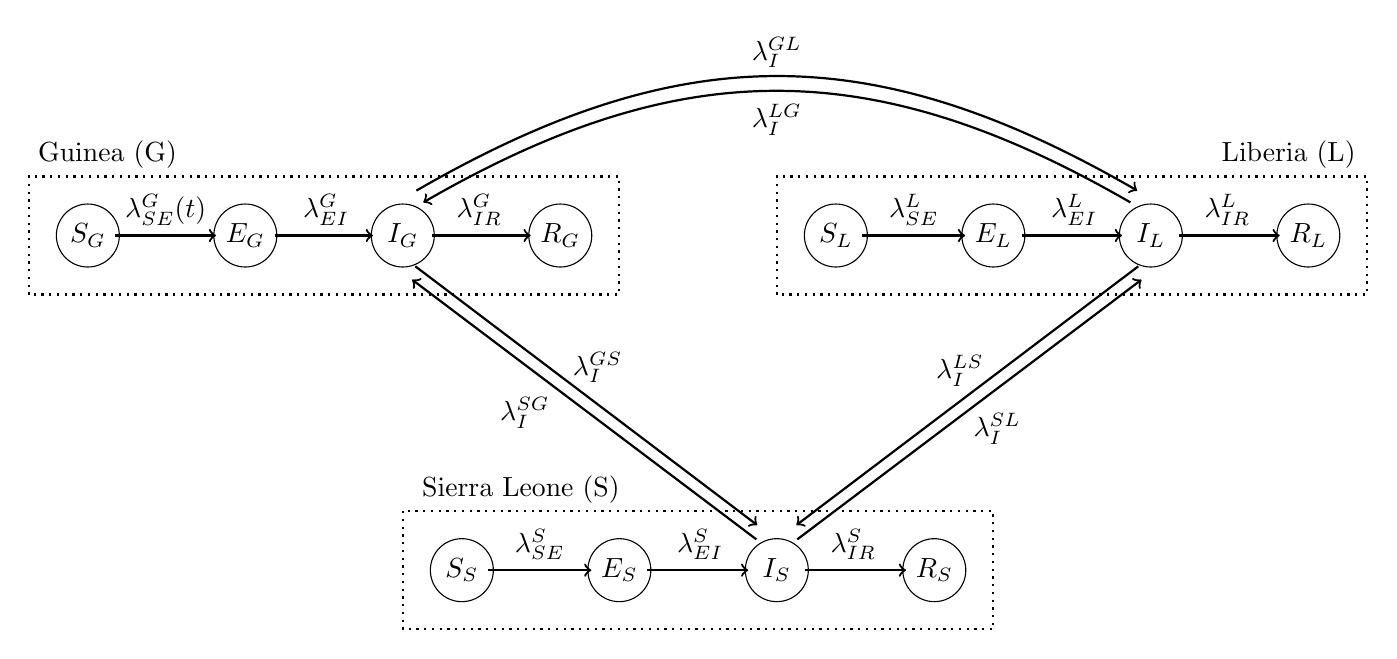
\begin{tikzpicture}
		\draw[thick,dotted] (0,-0.25) rectangle (7.5, 1.25);
		\node at (1, 1.1) [label=Guinea (G)] {};
		\draw (0.75, 0.5) circle(0.4) node (Sa) {$ S_G $};
		\draw (2.75, 0.5) circle(0.4) node (Ea) {$ E_G $};
		\draw (4.75, 0.5) circle(0.4) node (Ia) {$ I_G $};
		\draw (6.75, 0.5) circle(0.4) node (Ra) {$ R_G $};
		
		\draw[thick,dotted] (9.5,-0.25) rectangle (17, 1.25);
		\node at (16, 1.1) [label=Liberia (L)] {};	
		\draw (10.25, 0.5) circle(0.4) node (Sb) {$ S_L $};
		\draw (12.25, 0.5) circle(0.4) node (Eb) {$ E_L $};
		\draw (14.25, 0.5) circle(0.4) node (Ib) {$ I_L $};
		\draw (16.25, 0.5) circle(0.4) node (Rb) {$ R_L $};
		
		\draw[thick,dotted] (4.75,-3) rectangle (12.25, -4.5);
		\node at (6.25, -3.15) [label=Sierra Leone (S)] {};	
		\draw (5.5, -3.75) circle(0.4) node (Sc) {$ S_S $};
		\draw (7.5, -3.75) circle(0.4) node (Ec) {$ E_S $};
		\draw (9.5, -3.75) circle(0.4) node (Ic) {$ I_S $};
		\draw (11.5, -3.75) circle(0.4) node (Rc) {$ R_S $};
		
		\draw [thick,->] (Sa) -- (Ea) node[midway,above] {$ \lambda_{SE}^G(t) $};
		\draw [thick,->,shorten >=.6mm] (Ea) -- (Ia) node[midway,above] {$ \lambda_{EI}^G $};
		\draw [thick,->,shorten <=.5mm] (Ia) -- (Ra) node[midway,above] {$ \lambda_{IR}^G $};
		
		\draw [thick,->] (Sb) -- (Eb) node[midway,above] {$ \lambda_{SE}^L $};
		\draw [thick,->,shorten >=.6mm] (Eb) -- (Ib) node[midway,above] {$ \lambda_{EI}^L $};
		\draw [thick,->,shorten <=.5mm] (Ib) -- (Rb) node[midway,above] {$ \lambda_{IR}^L $};
		
		\draw [thick,->] (Sc) -- (Ec) node[midway,above] {$ \lambda_{SE}^S $};
		\draw [thick,->,shorten >=.6mm] (Ec) -- (Ic) node[midway,above] {$ \lambda_{EI}^S $};
		\draw [thick,->,shorten <=.5mm] (Ic) -- (Rc) node[midway,above] {$ \lambda_{IR}^S $};
		
		\path [thick, <-] ([yshift=-0.5mm,xshift=-2mm]Ia.south) edge [shorten >= 2mm, shorten <= 4mm] node [above,xshift=2.5mm,yshift=1.5mm] {$ \lambda_I^{GS} $} ([xshift=-1mm]Ic.north);
		\path [thick, ->] (Ia.south) edge [shorten >= 5mm, shorten <= 2mm] node [below,xshift=-9mm,yshift=2mm] {$ \lambda_I^{SG} $} ([xshift=1.5mm]Ic.north);
		
		\path [thick, <-] ([yshift=-0.5mm,xshift=2mm]Ib.south) edge [shorten >= 2mm, shorten <= 4mm] node[above,yshift=1mm,xshift=-2mm] {$ \lambda_I^{LS} $} ([xshift=1mm]Ic.north);
		\path [thick, ->] (Ib.south) edge [shorten >= 5mm, shorten <= 2mm] node[below,xshift=5mm] {$ \lambda_I^{SL} $} ([xshift=-1.5mm]Ic.north);
		
		\path [thick, <-] ([]Ia.north) edge [shorten >= 3mm, shorten <= 3mm, bend left, looseness=1.1] node [below] {$ \lambda_I^{LG} $} ([]Ib.north);
		\path [thick, ->] ([]Ia.north) edge [shorten >= 2mm, shorten <= 2mm, bend left, looseness=1.1,yshift=2mm] node [above] {$ \lambda_I^{GL} $} ([]Ib.north);	
		\end{tikzpicture}
	}
	\caption[Model diagram for a stratified SEIR model with country specific outbreak dynamics and cross--country transmission.]{Diagram of state transitions for a stratified SEIR model used in simulating an outbreak in Guinea, Liberia, and Sierra Leone. Dashed boxes denote countries, nodes in circles denote the model compartments: susceptible (S), exposed (E), infectious (I), recovered (R). Compartments  are subscripted with country indicators. Solid lines with arrows indicate stochastic transitions between model compartments, which occur continuously in time. Rates at which individuals transition between compartments are denoted by $ \lambda $ and are subscripted by compartments and superscripted by countries, e.g., $ \lambda_{SE}^L $ is the rate at which susceptible individuals become exposed in Liberia, $ \lambda_I^{SG} $ is the rate at which an infected individual in Sierra Leone migrates to Guinea. The rate at which susceptible individuals in Guinea become infected is time varying with one changepoint at 33 weeks.}
	\label{fig:stratified_seir_full_diag}
\end{figure}

\begin{table}[htbp]
	\caption[Week zero, and true and effective population sizes for a simulated Ebola outbreak in West Africa.]{True and effective population sizes, and initial conditions for a simulated outbreak in Guinea, Liberia, and Sierra Leone. Week zero is one week before the first observation is accrued and the time at which within--country transmission was assumed to begin. }
	\label{tab:ebola_synth_consts}
	\footnotesize
	\centering
	\begin{tabular}{lccc}	
		\hline	
		& \textbf{Guinea} & \textbf{Liberia} & \textbf{Sierra Leone} \\\hline
		\textbf{True population size $ (N)$} & 11.8 million & 4.4 million & 7.1 million \\ 
		\textbf{Effective population size $ (N_{eff}) $} & 15,000 & 35,000 & 25,000 \\
		\textbf{Week zero $ (t_0) $} & 0 & 10 & 19 \\
		\textbf{Initial state at $ t_0 $} $ (S_0,E_0,I_0,R_0) $ & (11.8$ \times 10^6$-7, 4, 3, 0) & (4.4$ \times 10^6$-5 3, 2, 0)& (7.1$ \times 10^6$-5, 3, 2, 0) \\
		\hline
		&&&
	\end{tabular} 
\end{table}

\begin{sidewaystable}[htbp]
	\begin{fullpage}
		\caption[Parameters and priors for a simulated Ebola outbreak in West Africa.]{Parameters under which the outbreak and data were simulated, prior distributions, and 95\% prior intervals. Subscripts, $ G,L,S, $ indicate specific countries, or generic countries $ A,B $ if a prior is shared. Effective reproduction numbers are defined with respect to the effective population size as $ R_{eff} = \beta N_{eff} /\mu $.}
		\label{tab:ebola_synth_pars}
		\scriptsize
	\centering
	\begin{tabular}{lclll}
		\hline
		\textbf{Parameter} & \textbf{Truth} & \textbf{Interpretation} & \textbf{Prior} & \textbf{Median (95\% Interval)} \\ \hline
		$ R_{eff,G}^{(1)}(t),\ t<33 $ & 1.3 & Effective reproduction \#  & $ R_{eff,G}^{(2)} / R_G^{(1)}\sim $ LogNormal(0, 0.5$ ^2 $) & $ R_{eff,G}^{(2)} / R_{eff,G}^{(1)} = $ 1.00 (0.38, 2.66) \\
		$ R_{eff,G}^{(2)}(t),\ t\geq33 $ & 1.1 & Effective reproduction \# & $ R_{eff,G}^{(2)}-1\sim $ LogNormal(log(0.5), 1.1) & $ \implies R_{eff,G}^{(2)} = 1.50 (1.06, 5.32)$ \\
		$ R_{eff,L} $ & 2.1 & Effective reproduction \# & $ R_{eff,L}\sim $ LogNormal(log(0.5), 1.1) & $ \implies R_{eff,L}^{(2)} = 1.50 (1.06, 5.32)$ \\
		$ R_{eff,S} $ & 1.6 & Effective reproduction \# & $ R_{eff,S}\sim $ LogNormal(log(0.5), 1.1) & $ \implies R_{eff,S}^{(2)} = 1.50 (1.06, 5.32)$ \\
		\makecell[l]{$ \alpha_{GS},\alpha_{GL}, \alpha_{LG},$\\
		$ \alpha_{LS},\alpha_{SG}, \alpha_{SL} $} & 0.003 & \makecell[l]{Infectious migration rate \\ from country A to B} & $ 1000\alpha_{AB} \sim$ Exponential(0.25) & \makecell[l]{\# migrations per 1000 infected \\ = 2.78 (0.10, 14.76)}\\ 
		$ \omega_G $ & 1.1 & Rate from $ E_G\rightarrow I_G $ & $ (1/\mu_G)\big/(1/\omega_G) \sim $ LogNormal(0.05, 0.35$ ^2 $) & $ (1/\mu_G)\big/(1/\omega_G) $ = 1.05 (0.53, 2.08) \\
		$ \omega_L $ & 0.8 & Rate from $ E_L\rightarrow I_L $ & $ (1/\mu_L)\big/(1/\omega_L) \sim $ LogNormal(0.05, 0.35$ ^2 $) & $ (1/\mu_L)\big/(1/\omega_L) $ = 1.05 (0.53, 2.08) \\
		$ \omega_S $ & 1.2 & Rate from $ E_S\rightarrow I_S $ & $ (1/\mu_S)\big/(1/\omega_S) \sim $ LogNormal(0.05, 0.35$ ^2 $) & $ (1/\mu_S)\big/(1/\omega_S) $ = 1.05 (0.53, 2.08) \\
		$ \mu_G $ & $ 1.1 $ & Rate from $ E_G\rightarrow I_G $ & $ 1/\mu_G\sim $ LogNormal(0, 0.5$ ^2 $) & $ 7/\mu_G = $ 7.0 (2.63, 18.65) \\
		$ \mu_L $ & $ 0.8 $ & Rate from $ E_L\rightarrow I_L $ & $ 1/\mu_L\sim $ LogNormal(0, 0.5$ ^2 $) & $ 7/\mu_L = $ 7.0 (2.63, 18.65) \\
		$ \mu_S $ & $ 1.2 $ & Rate from $ E_S\rightarrow I_S $ & $ 1/\mu_S\sim $ LogNormal(0, 0.5$ ^2 $) & $ 7/\mu_S = $ 7.0 (2.63, 18.65) \\
		$ N_{eff,G} $ & 15,000 & Effective population size & $ N_{eff,G}\sim\mr{Unif}(\sum_{\ell=1}^{L}Y_\ell^G, N_G/4) $& $ N_{eff,G} \in (4032,\ 2.95\times10^6) $ \\
		$ N_{eff,L} $ & 35,000 & Effective population size & $ N_{eff,L}\sim\mr{Unif}(\sum_{\ell=1}^{L}Y_\ell^L, N_L/4) $& $ N_{eff,L} \in (5945,\ 1.1\times10^6) $ \\
		$ N_{eff,S} $ & 25,000 & Effective population size & $ N_{eff,S}\sim\mr{Unif}(\sum_{\ell=1}^{L}Y_\ell^S, N_S/4) $& $ N_{eff,S} \in (9531,\ 1.775\times10^6) $ \\
		$ \rho_G $ & 0.85 & Mean case detection prob. & $ \logit(\rho_G) \sim $ LogNormal(0, 1.4$ ^2 $) & $ \implies \rho_G = 0.5, (0.06, 0.94)$ \\
		$ \rho_L $ & 0.2 & Mean case detection prob. & $ \logit(\rho_L) \sim $ LogNormal(0, 1.4$ ^2 $) & $ \implies \rho_L = 0.5, (0.06, 0.94)$ \\
		$ \rho_S $ & 0.6 & Mean case detection prob. & $ \logit(\rho_S) \sim $ LogNormal(0, 1.4$ ^2 $) & $ \implies \rho_S = 0.5, (0.06, 0.94)$ \\
		$ \phi_G,\ \phi_L, \phi_S $ & 50 & Neg.Binomial overdispersion & $ \log(\phi) \sim $ LogNormal(0, 5$ ^2 $) & $ \implies \rho_G = 1, (5.5\times 10^-5, 1.8\times10^4)$ \\
		\hline
	\end{tabular}
	\end{fullpage}
\end{sidewaystable}

\begin{table}
	\caption[Priors for initial compartment volumes for a simulated Ebola outbreak in West Africa]{Priors for the initial compartment volumes at the times when transmission commenced in each country for a simulated Ebola outbreak in West Africa. The initial compartment volumes for each country are assigned independent truncated multivariate normal priors that respect the boundary conditions on the state space of compartment volumes for that country (explained in Section \ref{sec:lna_init_volumes}). If he population size for country A is $ N_A $, and the initial state probability is denoted $ \bp_{0,A} = \bX_{0,A}/N_A  = (S_{0,A}, E_{0,A}, I_{0,A}, R_{0,A})/N_A$, the prior is a truncated multivariate normal approximation of a multinomial distribution with mean $ N_A\bp_{0,A}$ and covariance $ N_A(\bP_{0,A} - \bp_{0,A}\bp_{0,A}^T) $.} 
	\label{tab:ebola_synth_initdist_priors}
	\centering
	\begin{tabular}{lc}
		\hline \textbf{Country} & \textbf{Prior mean initial volumes} ($ \bX_0 $) \\
		\hline
		Guinea & ($ 11.8\times10^6 -7.1$, 4, 3, 0.1) \\
		Liberia & ($ 4.4\times10^6 -5.1$, 3, 2, 0.1) \\
		Sierra Leone & ($ 7.1\times10^6 -5.1$, 3, 2, 0.1) \\
		\hline
	\end{tabular}
\end{table}

\begin{table}
	\caption[Transmission rates for the stratified SEIR model with migration of infecteds for Ebola in West Africa.]{Rates of transitions between compartments for the full stratified SEIR model for the spread of Ebola in Guinea, Liberia, and Sierra Leone with cross--country migration of infected individuals across country borders. These rates were used in simulating the outbreak and data, and in the supplementary model presented in Section \ref{subsec:ebola_synth_fullmod_res}. The model is diagrammed in Figure \ref{fig:stratified_seir_full_diag}. Subscripts in the rates denote model compartments, superscripts denote countries. Subscripts for parameters denote countries. The rate at which susceptibles in Guine become infected is time varying with one changepoint at 33 weeks. Transmission in Liberia and Sierra Leone prior to weeks 10 and 19 is expressed in the initial compartment volumes at those times. Thus, all respective transition rates are set to zero prior to the times when transmission commenced in those countries.}
	\label{tab:ebola_synth_rates_full}
	\centering\footnotesize
	\begin{tabular}{llll}
		\hline
		\textbf{From} & \textbf{To} & \textbf{Country} & \textbf{Rate} \\
		\hline
		Susceptible & Exposed & Guinea & $ \lambda_{SE}^G(t) = (\beta_G^{(1)} \ind{t<33} + \beta_G^{(2)}\ind{t\geq33})S_GI_G $ \\
		Susceptible & Exposed & Liberia & $ \lambda_{SE}^L = \beta_L\ind{t\geq10}S_LI_L $\\
		Susceptible & Exposed & Sierra Leone & $ \lambda_{SE}^S = \beta_S\ind{t\geq19}S_SI_S $ \\
		Exposed & Infected & Guinea & $ \lambda_{EI}^G = \omega_GE_G $\\
		Exposed & Infected & Liberia & $ \lambda_{EI}^L = \omega_L\ind{t\geq10}E_L $ \\
		Exposed & Infected & Sierra Leone & $\lambda_{EI}^S = \omega_S\ind{t\geq19}E_S$ \\
		Infected & Recovered & Guinea & $ \lambda_{IR}^G = \mu_GI_G $ \\
		Infected & Recovered & Liberia & $ \lambda_{IR}^L = \mu_L\ind{t\geq10}I_L $ \\	
		Infected & Recovered & Sierra Leone & $ \lambda_{IR}^S = \mu_S\ind{t\geq19}I_S $ \\
		Infected (A) & Infected (B) & Countries A,B & $ \lambda_I ^{AB} = \alpha_{AB}\ind{t\geq{t_{0}^A}}\ind{t\geq t_{0}^B}I_A$\\
		\hline
	\end{tabular}
\end{table}

\begin{table}
	\caption[Transmission rates for the stratified SEIR model with virtual migration of infecteds for Ebola in West Africa.]{Approximate rates of transitions between compartments for the stratified SEIR model for the spread of Ebola in Guinea, Liberia, and Sierra Leone with cross--country transmission via virtual migration of infected individuals. These rates were used in the primary model presented in Section \ref{subsec:ebola_synth}. The model is diagrammed in Figure \ref{fig:stratified_seir_full_diag}. Subscripts in the rates denote model compartments, superscripts denote countries. Subscripts for parameters denote countries. The rate at which susceptibles in Guine become infected is time varying with one changepoint at 33 weeks. Transmission in Liberia and Sierra Leone prior to weeks 10 and 19 is expressed in the initial compartment volumes at those times. Thus, all respective transition rates are set to zero prior to the times when transmission commenced in those countries.}
	\label{tab:ebola_synth_rates_approx}
	\centering\footnotesize
	\begin{tabular}{llll}
		\hline
		\textbf{From} & \textbf{To} & \textbf{Country} & \textbf{Rate} \\
		\hline
		Susceptible & Exposed & Guinea & \hspace{-0.7in}\makecell{$ \lambda_{SE}^G(t) = (\beta_G^{(1)} \ind{t<33} + \beta_G^{(2)}\ind{t\geq33})\times $\\
		\hspace{1.25in}$ (I_G + \alpha_{LG}\ind{t\geq10}I_L + \alpha_{SG}\ind{t\geq19}I_S)S_G $} \\
		Susceptible & Exposed & Liberia & $ \lambda_{SE}^L = \beta_L\ind{t\geq10}(I_L + \alpha_{GL}I_G + \alpha_{SL}\ind{t\geq19}I_S)S_L $\\
		Susceptible & Exposed & Sierra Leone & $ \lambda_{SE}^S = \beta_S\ind{t\geq19}(I_S + \alpha_{GS}I_G + \alpha_{LS}I_L)S_S $ \\
		Exposed & Infected & Guinea & $ \lambda_{EI}^G = \omega_GE_G $\\
		Exposed & Infected & Liberia & $ \lambda_{EI}^L = \omega_L\ind{t\geq10}E_L $ \\
		Exposed & Infected & Sierra Leone & $\lambda_{EI}^S = \omega_S\ind{t\geq19}E_S$ \\
		Infected & Recovered & Guinea & $ \lambda_{IR}^G = \mu_GI_G $ \\
		Infected & Recovered & Liberia & $ \lambda_{IR}^L = \mu_L\ind{t\geq10}I_L $ \\	
		Infected & Recovered & Sierra Leone & $ \lambda_{IR}^S = \mu_S\ind{t\geq19}I_S $ \\
		\hline
	\end{tabular}
\end{table}

\subsection{MCMC Details}
\label{subsec:ebola_synth_mcmc}
We fit two models to the simulated data, the true model where migration was modeled explicitly and the approximated model, described in Section \ref{subsec:ebola_synth}, where cross--border transmission was incorporated into the rate of infection via virtual migration. The model fitting procedure and priors were the same for both models. We ran five chains for each model, initialized at random parameter values, for 200,000 iterations per chain. The model parameters, not including the initial compartment volumes, were jointly updated via MVNSS (see Section \ref{subsubsec:mvn_slice_sampling}). The empirical covariance for the MVNSS algorithm was update over the first 100,000 iterations using the gain factor sequence, $\gamma_n = 0.5(1 + 0.01n)^{-0.9}$. The contribution of isotropic Gaussian noise to the proposal was initialized at 0.001 and reduced throughout the adaptation phase according to the sequence $ \iota_n = 0.001(1 + 0.01n)^{-0.99} $. The covariance matrix was blocked by country with covariances for parameters belonging to different countries set to zero. Thus, country specific parameters were proposed jointly but were independent in the proposal. Migration parameters were blocked with parameters corresponding to the destination country. The initial compartment volumes were updated jointly with the LNA paths in an EllipSS step. The MCMC alternated between three ElliptSS and two MVNSS updates per MCMC iteration. The ElliptSS bracket width was reset after the first 5,000 MCMC iterations to $ \omega = 2\sqrt{2\log(10)}\sigma_{ElliptSS}$, where $ \sigma_{ElliptSS} $ was the standard deviation of the accepted angles over the initial iterations. The MCMC estimation scales for each country were parameterized as in Table \ref{tab:seir_params_est3} with the one addition being the log ratio of effective reproductive numbers, subtract one, for Guinea, $ \log\left ((R_{eff,G}^{(2)}-1)/(R_{eff,G}^{(1)}-1)\right ) $. Convergence was assessed using potential scale reduction factors (PSRFs) \cite{brooks1998general}, computed via the \texttt{coda} R package \cite{codapackage}. PSRFs were less than 1.05 in all cases.

\subsection{Additional Results and Diagnostics}
\label{subsec:ebola_synth_supplement}

\newpage
\subsection{Supplementary Results with Explicit Migration of Infected Individuals}
\label{subsec:ebola_synth_fullmod_res}

\section{LNA Implementation Details and LNA Model Vignettes}
\label{sec:lna_implementation_vignettes} % Bayesian computation

\end{document}
